\documentclass[msc, classic, a4paper]{ufbathesis}
\usepackage[utf8]{inputenc}
\usepackage[brazil]{babel}
\usepackage{fancyvrb}
\usepackage[alf]{abntex2cite}
\usepackage{multicol}
\usepackage{acronym}
\usepackage{listings}
\usepackage{float}

\defenseyear{2016}
\date{08 de Julho de 2016}
\adviser[f]{Profa. Dra. Christina von Flach G. Chavez}
\coadviser{Prof. Dr. Paulo Roberto Miranda Meirelles}

\title{
  Softwares acadêmicos de origem científica:
  ``dysfunctional chaotic churn'' em projetos de análise estática
}

\author{Joenio Marques da Costa\\
  {\small joenio@joenio.me}
}

\begin{document}

\frontpage
\frontmatter
\presentationpage

\resumo

(pendente)

\begin{keywords}

  (pendente)

\end{keywords}

\tableofcontents
\listoffigures
\listoftables
\chapter*{Glossário}

\begin{acronym}[Sustentabilidade de software]
  \acro{analise-estatica-de-software}[Análise estática de software]{
    É o processo de coleta de informações de um software a respeito dos seus
    componentes e sua organização interna sem necessidade de execução do código
    fonte.
  }
  \acro{disponibilidade}[Disponibilidade]{
    Capacidade de um softwares estar acessível publicamente para obtenção no
    presente.
  }
  \acro{manutenabilidade}[Manutenabilidade]{
    Característica de qualidade de software que indica o quão fácil é
    realizar atividades de evolução e manutenção em seu código fonte.
  }
  \acro{reprodutibilidade}[Reprodutibilidade]{
    Capacidade de reprodução de um dado estudo científico, ou seja, recriar
    o espírito do que outra pessoa fez, usando seus próprios artefatos.
  }
  \acro{software-academico}[Software acadêmico]{
    Softwares desenvolvidos durante pesquisas científicas, sejam pequenos
    scripts, protótipos ou produtos maduros, que tenham sido utilizados durante
    o estudo para coleta, extração ou análise dos dados (podem ser encontrados
    com o nome de {\it research-originated software} ou {\it research tool}).
  }
  \acro{sustentabilidade-de-software}[Sustentabilidade]{
    Conceito guarda chuva composto de múltiplas dimensões, social, individual,
    ambiental, econômica e técnica, que traz o tema sustentabilidade para o campo da
    ciência da computação exibindo preocupação com os impactos que os sistemas
    e a tecnologia da informação causam no futuro do planeta.
  }
  \acro{sustentabilidade-tecnica}[Sustentabilidade técnica]{
    Dimensão da sustentabilidade preocupada com a longevidade da informação,
    dos sistemas, e infraestrutura, e sua adequada evolução frente as condições
    do ambiente em constante mudança.
  }
\end{acronym}

\mainmatter

%------------------------------------------%

\xchapter{Introdução}{}

"Ocorrências não reprodutíveis não têm significado para a ciência" \cite{popper2004logica}.

\section{Motivação}

Em 2010, ... contar o cenário que envolve Analizo.

Eu, como engenheiro de software pesquisador e parte do ecossistema do software
acadêmico de análise estática Analizo estou interessado em saber como melhor
investir recursos no ecossistema do projeto Analizo com o objetivo de fazê-lo
mais útil e acessível para todo o campo de pesquisa, uma vez que percebo que os
projetos de software do meu campo sofrem da existência de muitos projetos, com
poucos usuários, com ciclos de vida curtos, que terminam em paralelo ao
financiamento inicial, comunidades desconectadas e paralelas,
incompatibilidades entre projetos, e tentativas aparentemente não coordenadas
de ``reiniciar'' tudo ({\it re-boots}).

Mas antes de saber como atingir este objetivo é necessário compreender como
este problema ocorre e se ele realmente acontece no ecossistema de software
acadêmico de análise estática.

% é interessante realmente apresentar o Analizo como um case de sucesso

%software acadêmicos sofrem de {\it ``dysfunctional chaotic churn''}.
% O ecossistema de software acadêmico sofre de um fenômeno chamado de
% desordem caótica disfuncional ({\it ``dysfunctional chaotic churn''}).

\section{Apresentação}

A Ciência moderna depende de software. Novos softwares são constantemente
criados e desenvolvidos durante pesquisas científicas, seja pelo próprio pesquisador,
seja por colaboradores. 
Estes softwares resolvem problemas comuns de pelo menos metade dos cientistas 
de todas as áreas da Ciência, em atividades de coleta ou análise, 
e em outras atividades de pesquisa.

Estes softwares variam em tamanho e finalidade: alguns são simples
scripts para automatizar tarefas repetitivas, enquanto outros são utilizados para
coleta, análise ou transformação de dados. Alguns softwares são projetos maduros e
carregam boa parte do conhecimento desenvolvido ao longo da própria pesquisa, e
costumam ter uma maior promoção por parte dos seus autores e um maior
reconhecimento por parte da comunidade científica.

O domínio e objetivo da pesquisa também implicam em particularidades do software: 
um software para coleta de dados numa pesquisa em engenharia de
software certamente terá características e requisitos distintos de um software
para o mesmo fim em outro domínio, por exemplo,  antropologia ou medicina.
Em um mesmo domínio, softwares para análise de dados podem variar
enormemente entre sí, dependendo do objetivo da pesquisa e das atividades realizadas.
\'{E} natural acreditar, portanto, que existe demanda suficiente para a
criação de softwares para os mais diversos campos de atuação e aplicação da
Ciência.

A criação destes softwares tem motivações variadas:  alguns cientistas publicam
seus softwares juntamente com dados e outros artefatos, outros fazem um esforço
adicional para documentar e incentivar o seu uso e adoção, alguns não
consideram seus softwares dignos de publicação, outros não dão visibilidade a
sua existência mesmo quando são publicados sob as melhores práticas da
engenharia de software.

Independente da finalidade, tamanho ou motivação, todo software tem o potencial
de voltar a ser útil em outros momentos ou lugares, para o autor original,
ou para pesquisadores enfrentando problemas semelhantes aos dos autores originais.
Não é difícil imaginar que o problema enfrentado por um pesquisador pode, em
algum momento, ser enfrentado por outros pesquisadores, criando assim uma ótima
oportunidade de colaboração entre pesquisas e pesquisadores, sendo o software
um excelente vetor de ajuda mútua em ambas as direções.

Apesar disso, cientistas tem percebido que os softwares desenvolvidos na
academia sofrem de {\it ``dysfunctional chaotic churn''}, ou seja, a existência
de muitos projetos, com poucos usuários, com ciclos de vida curtos, que
terminam em paralelo ao financiamento inicial, comunidades desconectadas e
paralelas, incompatibilidades entre projetos, e tentativas aparentemente não
coordenadas de ``reiniciar'' tudo ({\it re-boots}).

%Este cenário, além de desacelerar o progresso geral da ciência gerando
%retrabalho, faz surgir questionamentos sobre as conclusões dessas pesquisas,
%especialmente quando grande parte dos pesquisadores não sabem o quão confiável
%seus softwares são.

Este problema apesar de ser percebido por muitos cientistas carece de
evidências, neste trabalho investigamos como ele se manifesta em pesquisas da
engenharia de software, em especial, em publicações de análise estática, uma
área com uma longa e respeitável tradição em pesquisas sobre a criação de novas
ferramentas, métodos e algoritmos.

\section{Escopo}

O objetivo geral desta pesquisa é explorar como o {\it ``dysfunctional chaotic
churn''} se manifesta entre os projetos de software de análise estática,
respondendo as seguintes questões:

\begin{itemize}
  \item Projetos de software acadêmico de análise estática tem contribuidores além dos autores iniciais?
  \item Os projetos incentivam ativamente a contribuição?
  \item Os espaços dos projetos são abertos e transparentes?
  \item Os projetos fazem um pedido explícito e claro de reconhecimento?
\end{itemize}

Que tal perguntas assim?
\begin{itemize}

  \item Os projetos sustentáveis tem contribuidores além dos autores iniciais?
  \item Os projetos sustentáveis tem mais contribuidores?
  \item Os artigos de projetos sustentáveis são mais lidos, mais citados?
  \item Os autores de projetos sustentáveis tem mais publicações com o uso de software do que os autores?
  \item Os projetos são mais fáceis de manter?  de usar? 
\end{itemize}



Estas questões darão importantes indícios sobre a qualidade do software acadêmico de
análise estática desenvolvido na academia, especialmente sobre a capacidade de serem 
encontrados, compartilhados e co-desenvolvidos.

\section{Metodologia de trabalho}

(apresentar aqui um resumo do capítulo \ref{metodologia})

Objetivo específico: caracterizar software acad publicado quanto a ...
Objetivo específico: caracterizar o tipo de citação / menção d
  \item Os projetos tem contribuidores além dos autores iniciais?
  \item Os projetos incentivam ativamente a contribuição?
  \item Os espaços dos projetos são abertos e transparentes?
  \item Os projetos fazem um pedido explícito e claro de reconhecimento?

\section{Contribuições}

(pendente)

\section{Organização do texto}

(pendente)

%O capítulo \ref{fundamentacao} apresenta os fundamentos teóricos necessários
%para a compreensão deste trabalho.
%
%O capítulo \ref{metodologia} apresenta a estratégia de pesquisa adotada nos
%estudos.
%
%O capítulo \ref{sustentabilidade-tecnica} traz um estudo sobre a
%sustentabilidade técnica e a disponibilidade dos softwares acadêmicos de
%análise estática.
%
%O capítulo \ref{complexidade-ferramentas} descreve um estudo sobre a
%manutenabilidade dos softwares acadêmicos de análise estática.
%
%O capítulo \ref{conclusoes} apresenta as considerações finais e discute os
%resultados deste trabalho.

% A Retrospective Study of Academic Software Projects
% (estudo restropectivo parece um bom termo, uma busca rápida no google-scholar retornou muita coisa da área de saúde)

                            % motivation

%------------------------------------------%

% A Preliminary Literature Review which indicates: 
% (i) that you have studied the work of the major authors in your research field 
% (ii) that you are familiar with the major themes relevant to that subject area 
% (iii) what further investigations you intend to pursue as part of this dissertation. 
% You should bear in mind that you are reviewing the literature in order to develop sharper, 
% more insightful and focused research questions about your topic. 
% Therefore, your literature review should lead to and justify your research objectives and questions.

% continuar a partir de:
% /home/joenio/src/bibliografia/Papers/Replication of Controlled Experiments in Empirical Software Engineering - A Survey.pdf

\xchapter{Fundamentação teórica}
{Este capítulo apresenta conceitos necessários para a compreensão do trabalho.}
\label{fundamentacao}

%\section{Software acadêmico}
%
%% Anúncio em destaque no ACM DL: Reproducibility of Results in the ACM Digital Library 
%% http://dl.acm.org/docs/reproducibility.cfm
%
%% ciencia aberta e desenvolvimento sustentavel
%% https://ocsdnet.org/open-and-collaborative-science-using-knowledge-as-a-pathway-to-sustainable-development/
%
%Segundo \citeonline{hettrick_2014_14809} software acadêmico ({\it research
%software}) é todo software usado para gerar, processar ou analisar resultados
%de pesquisas com intenção de ser publicados (seja num jornal, revista,
%conferência, monografia, livro ou tese). Software de pesquisa pode ser qualquer
%coisa entre poucas linhas escritas por você mesmo, até mesmo um software
%desenvolvido profissionalmente. Software que não gera, processa ou analisa
%resultados - como por exemplo um editor de textos, ou o uso de navegadores web
%- não são considerados softwares de pesquisa, segundo esta definição.
%
%%% Softwares acadêmicos são softwares desenvolvidos no decorrer de pesquisas
%%% científicas como parte de um estudo a ser publicado (seja num jornal, revista,
%%% conferência, monografia, livro ou tese), podem ser pequenos scripts contendo
%%% poucas linhas de código, protótipos, ou mesmo produtos de software completos
%%% que demonstram ou refletem os resultados de uma pesquisa, costumam ser
%%% utilizados para gerar, processar ou analisar resultados, mas podem ser para
%%% qualquer outro fim, basta que seja um dos artefatos gerado na pesquisa, será
%%% considerado software acadêmico.
%%% 
%%% Tais softwares podem ser encontrados na literatura pelo nome de {\it research
%%% tool} \cite{Portillo12}, {\it research-originated software} \cite{Kon2011},
%%% %{\it research software} \cite{hettrick_2014_14809} ou
%%% {\it academic software} \cite{allen2017engineering}, e costumam ser citados
%%% pelos seus autores como uma contribuição do estudo, seja principal ou
%%% secundária, alguns autores criam softwares acadêmicos como meio para atingir os
%%% resultados da pesquisa e não descrevem muito bem o software.
%%% 
%%% %, traduzido para software acadêmico para evitar o
%%% %termo {\it software de pesquisa}, a palavra {\it research} em português {\it
%%% %pesquisa} pode ser facilmente confundida com ferramentas ou sistemas de
%%% %pesquisa, como sites de pesquisa por exemplo,
%%% 
%%% % este artigo \cite{howison2016software} faz exatamento o mesmo estudo que estou fazendo!
%%% 
%%% Copiar e usar exatamente esta linha de pensamento e argumentos:
%%% Yet, the visibility of software in the scientific record is in
%%% question, leading to concerns, expressed in a series of
%%% National Science Foundation (NSF)- and National Institutes
%%% of Health–funded workshops, about the extent that scientists
%%% can understand and build upon existing scholarship (e.g.,
%%% Katz et al., 2014; Stewart, Almes, & Wheeler, 2010). In
%%% particular, the questionable visibility of software is linked to
%%% concerns that the software underlying science is of question-
%%% able quality. These quality concerns are not just technical,
%%% but extend to the appropriateness of software for wide
%%% sharing, and its ability to facilitate the codevelopment that
%%% would make efficient use of limited scholarly funding
%%% (Howison & Herbsleb, 2013; Katz et al., 2014).
%%% The link is two-fold: First, when software is not visible, it
%%% is often excluded from peer review; second, its lack of
%%% visibility, or the particular form of visibility, means that
%%% incentives to produce high-quality, widely shared, and code-
%%% veloped software may be lacking. A well-functioning system
%%% would assist not only the goals of understanding and trans-
%%% parency, but also the goals of aiding replication (Stodden
%%% et al., 2010), complementing the availability of publications
%%% such that “the second researcher will receive all the benefits
%%% of the first researcher’s hard work” (King, 1995, p. 445).
%%% The situation with software is broadly analogous (but not
%%% identical) to that of data in publications; indeed, all data are
%%% processed by software in some form (Borgman et al., 2012).
%%% Nonetheless, there are relevant differences. Accordingly, our
%%% inquiry into the visibility of software in scholarly commu-
%%% nication is complementary to recent interest in data citation.
%%% In sum, then, the relationship of software to the scholarly
%%% 
%%% 
%%% Como não existe ainda amadurecimento suficiente sobre como citar softwares e
%%% outros artefatos em pesquisas científicas, não temos um padrão de como fazê-lo,
%%% cada autor cita à sua maneira, muitas vezes ao longo do texto, outras em seções
%%% específicas sobre a implementação do software, nem semprem informam onde
%%% encontrar uma cópia do software, ou ainda nem sobre o modelo em que o software
%%% é distribuído, ou se é de alguma forma distribuído ao público.
%%% 
%%% Os softwares acadêmicos neste estudo serão aquelas citados pelo autor como
%%% contribuição do estudo, então toda vez que citarmos software acadêmico estamos
%%% falando de artefatos de software citados pelo autor como contribuição do estudo.

\section{Ciência aberta}

Over the past fifteen years the scholarly communications agenda
has progressed gradually. Currently we are experiencing a strong
tendency among all research stakeholders to engage with the
practice of OS. Lately, research funders require the sharing not
only of the research results they have funded, but also of the
procedures and data that are being generated during the research
conduct. Researchers, on the other side, are keen on observing
their research results being used for the improvement of the
society and are forced by their funders to demonstrate the impact
of their research. At the same time, higher academic institutions
aim to join the OS agenda as well, since they see the opportunity
of great economic benefits and savings. While OS is the possible
answer to all these factors, the stakeholders’ inability to
understand the requirements for the application of OS can be a
suspensory factor for the OS implementation and evolution.
The aim of the FOSTER project is to advance the stakeholders'
knowledge on the usefulness of OS and explain the technicalities,
strategies and best practices using which OS can be applied. As an
attempt to educate the largest number of researchers possible,
FOSTER has created an e-leanring portal, which contains quality
assured information relating to the topic and it is open to everyone
in the world. The platform contains two types of information:
learning material and online courses. The classification of these
two types is supported by an OS taxonomy, where related terms
are applied both in the portal's material and also in the courses.
With the use of the taxonomy, users are in the position to
understand the OS domain and the concepts around it.
The main goal of the FOSTER project, which is mainly achieved
through the portal functionalities, is not only to educate the
research stakeholders on OS, but also to build a community of
researchers, librarians, software developers, funders and research
administrators who are interested in OS in order to advance the
way research is being conducted and shared. In addition, FOSTER
attempts to provide tools to this community, such as re-usable
content for training and a platform for blended learning and e-
learning courses that the community could run. This OS
advancement is essential for the research promotion and,
consequently, for the benefit of the society as a whole
\cite{Nancy2015}.

Open Science may be practised both
for philosophical and pragmatic reasons. As the
resources produced by open projects are
potentially accessible to public audiences, Open
Science offers both a novel medium for public
access and involvement in the process of science
and an innovative method for real-time science
communication. Does such direct access clear
the stream of communication or muddy the
waters with unfocussed, unclear and unvetted
comment? This paper suggests that adopting an
Open Science approach allows the capture of an
authentic and clear record of research.
However, researchers acknowledge this involves
opening their work up to a different type of
scrutiny \cite{Grand2010}.

Open Science is an emerging approach to the conduct of science, technology and engineering
projects, in which information about the whole of an ongoing investigation is made available
on and through the Internet. Adopting an Open Science approach means the audience for the
research can extend beyond the researchers involved to other researchers and to members of
the public. Thus, Open Science has implications for engineering research, practice,
publishing and public engagement with engineering. This paper reviews the history and
evolution of the Open Science movement, includes some reflections on the related areas of
Open Access, peer-review and public engagement with science and engineering and discusses
data gathered from interviews. The analysis suggests that interviewees have concerns about
issues such as precedence and protection of original work and the time needed to integrate
open science practices into daily work. Successfully working in such collaborations is likely
to require not only common practical tools but also the development of shared language and
understanding between researchers and members of the public. Interviewees recognise the
value of Open Science in collaborative research and its innovative facility to sustain direct
public access to research outputs. It also has the potential to allow members of the public to
make real practical contributions to research \cite{Grand2010Open}.

This white paper was written as a contribution to the “Imagining
Tomorrow’s University: Rethinking scholarship, education, and institu-
tions for an open, networked era” workshop, a joint NIH/NSF-funded
event held 8–9 March 2017 in Rosemont, IL. In this paper, I present an
overview of what I consider open science, its importance, and how it
plays a role in my research agenda. I also discuss challenges faced in
pursuing research openness, and recommend changes to university
leaders to address these barriers \cite{niemeyer2017open}.

Open to All?  Case studies of openness in research
Since the early 1990s, the open access movement has promoted the concept of openness in relation
to scientific research. Focusing initially upon the records of science in the form of the text of articles
in scholarly journals, interest has broadened in the last decade to include a much wider range of
materials produced by researchers. At the same time, concepts of openness and access have also
developed to include various kinds of use, by machines as well as humans.
Academic bodies, including funders and groups of researchers, have set out statements in support
of various levels of openness in research. Such statements often focus upon two key dimensions:
what is made open, and how; and to whom is it made open, and under what conditions? This study
set out to consider the practice of six research groups from a range of disciplines in order to better
understand how principles of openness are translated into practice \cite{Nesta2010}.

\section{Reprodutibilidade}


The lack of replicability and reproducibility of scientific studies based on
computational methods has lead to serious mistakes in published scientific
findings, some of which have been discovered and publicized recently. Many
strategies are currently pursued to improve the situation. This article reports the
first conclusions from the ActivePapers project, whose goal is the development
and application of a computational platform that allows the publication of
computational research in a form that enables installation-free deployment,
encourages reuse, and permits the full integration of datasets and software into
the scientific record. The main finding is that these goals can be achieved with
existing technology, but that there is no straightforward way to adapt legacy
software to such a framework \cite{hinsen2014activepapers}

Reproducibility verification is essential to the practice of the scientific method.
Researchers report their findings, which are strengthened as other independent groups
in the scientific community share similar outcomes. In the many scientific fields
where software has become a fundamental tool for capturing and analyzing data, this
requirement of reproducibility implies that reliable and comprehensive software platforms
and tools should be made available to the scientific community. The tools will empower
them and the public to verify, through practice, the reproducibility of observations that
are reported in the scientific literature. Medical image analysis is one of the fields in
which the use of computational resources, both software and hardware, are an essential
platform for performing experimental work. In this arena, the introduction of the Insight
Toolkit (ITK) in 1999 has transformed the field and facilitates its progress by accelerating
the rate at which algorithmic implementations are developed, tested, disseminated and
improved. By building on the efficiency and quality of open source methodologies, ITK has
provided the medical image community with an effective platform on which to build a daily
workflow that incorporates the true scientific practices of reproducibility verification. This
article describes the multiple tools, methodologies, and practices that the ITK community
has adopted, refined, and followed during the past decade, in order to become one of the
research communities with the most modern reproducibility verification infrastructure. For
example, 207 contributors have created over 2400 unit tests that provide over 84% code
line test coverage. The Insight Journal, an open publication journal associated with the
toolkit, has seen over 360,000 publication downloads. The median normalized closeness
centrality, a measure of knowledge flow, resulting from the distributed peer code review
system was high, 0.46 \cite{McCormick2014}.

Linked Open Science—Communicating, Sharing and Evaluating
Data, Methods and Results for Executable Papers.
Linked Open Science is an approach to solve challenges of an executable paper. It is a combination of four “silver
bullets”: 1) publication of scientific data, metadata, results, and provenance information using Linked Data principles,
2) open source and web-based environments for executing, validating and exploring research, 3) Cloud Computing
for efficient and distributed computing, and 4) Creative Commons for the legal infrastructure. We will use a realistic
scientific research setting related to research on deforestation of the Brazilian Amazon rainforest to provide scenarios
to illustrate the application of Linked Open Science \cite{Kauppinen2011}.

Among empirical software engineering studies, those based on data re-
trieved from development repositories (such as those of source code management,
issue tracking or communication systems) are specially suitable for reproduction.
However their reproducibility status can vary a lot, from easy to almost impossible
to reproduce. This paper explores which elements can be considered to characterize
the reproducibility of a study in this area, and how they can be analyzed to better
understand the type of reproduction studies they enable or obstruct. One of the
main results of this exploration is the need of a systematic approach to asses the
reproducibility of a study, due to the complexity of the processes usually involved,
and the many details to be taken into account. To address this need, a methodology
for assessing the reproducibility of studies is also presented and discussed, as a tool to
help to raise awareness about research reproducibility in this field. The application
of the methodology in practice has shown how, even for papers aimed to be
reproducible, a systematic analysis raises important aspects that render reproduction
difficult or impossible. We also show how, by identifying elements and attributes
related to reproducibility, it can be better understood which kind of reproduction
can be done for a specific study, given the description of datasets, methodologies and
parameters it uses \cite{gonzalez2012reproducibility}.


Science rests on peer review and the wide-spread dissemination of
knowledge. Software engineering research will advance further and
faster if the sharing of data and tools were easier and more wide-
spread. Pragmatic concerns hinder the realization of this ideal: the
time and effort required and the risk of being scooped. We examine
the costs and benefits of facilitating sharing in our field in an effort
to help the community understand what problems exist and find
a solution. We examine how other fields, such as medicine and
physics, handle sharing, describe the value of sharing for replication
and innovation, and address practical concerns such as standards
and warehousing. To launch what we hope will become an ongoing
discussion of solutions in our community, we present some ways
forward that mitigate the risk of sharing — partial sharing, registry,
escrow, and market \cite{barr2010shoulders}.

Computer systems research spans sub-disciplines that in-
clude embedded and real-time systems, compilers, network-
ing, and operating systems. Our contention is that a number
of structural factors inhibit quality research. We highlight
some of the factors we have encountered in our work and ob-
served in published papers and propose solutions that could
both increase the productivity of researchers and the quality
of their output \cite{Vitek2011}.

At various machine learning conferences, at
various times, there have been discussions
arising from the inability to replicate the
experimental results published in a paper.
There seems to be a wide spread view that we
need to do something to address this prob-
lem, as it is essential to the advancement
of our field. The most compelling argument
would seem to be that reproducibility of ex-
perimental results is the hallmark of science.
Therefore, given that most of us regard ma-
chine learning as a scientific discipline, being
able to replicate experiments is paramount.
I want to challenge this view by separating
the notion of reproducibility, a generally de-
sirable property, from replicability, its poor
cousin. I claim there are important differ-
ences between the two. Reproducibility re-
quires changes; replicability avoids them. Al-
though reproducibility is desirable, I contend
that the impoverished version, replicability,
is one not worth having \cite{drummond2009replicability}.

Abstract—This paper is the result of reviewing all papers
published in the proceedings of the former International
Workshop on Mining Software Repositories (MSR) (2004-2006)
and now Working Conference on MSR (2007-2009). We have
analyzed the papers that contained any experimental analysis
of software projects for their potentiality of being replicated.
In this regard, three main issues have been addressed: i) the
public availability of the data used as case study, ii) the public
availability of the processed dataset used by researchers and iii)
the public availability of the tools and scripts. A total number of
171 papers have been analyzed from the six workshops/working
conferences up to date. Results show that MSR authors use
in general publicly available data sources, mainly from free
software repositories, but that the amount of publicly available
processed datasets is very low. Regarding tools and scripts, for
a majority of papers we have not been able to find any tool,
even for papers where the authors explicitly state that they have
built one. Lessons learned from the experience of reviewing the
whole MSR literature and some potential solutions to lower the
barriers of replicability are finally presented and discussed
\cite{robles2010replicating}.



Enquanto pesquisadores publicam artigos descrevendo e divulgando seus
resultados, é raro que façam o mesmo com toda a produção gerada durante a
pesquisa. A maioria dos componentes necessários para a reprodução dos
resultados de uma pesquisa -- por exemplo, códigos fonte e dados -- usualmente
permanecem não publicados. Esse problema fere um dos fundamentos
da ciência de que novas descobertas sejam reproduzidas antes de serem
consideradas parte da base de conhecimento \cite{Stodden2009}.

% Software Carpentry: lessons learned [version 2; referees: 3 approved]
%
% iniciativa voltada a melhorar as habilidades com computação entre os
% pesquisadores de diversas áreas, ajudando a melhorar os resultados,
% facilitar reprodutiblidade, acesso a dados, codigos, etc... reducao de custos
% melhoria de qualidade, etc... faz workshops, eventos, treinamentos, ao longo
% dos varios anos de existencia, ...
%
% Since its start in 1998, Software Carpentry has evolved from a week-long
% training course at the US national laboratories into a worldwide volunteer effort
% to improve researchers' computing skills. This paper explains what we have
% learned along the way, the challenges we now face, and our plans for the
% future.


Nesse sentido, \citeonline{Prlic2012} enfatizam que disponibilizar o código
criado durante pesquisas não apenas aumenta o impacto como também se torna
essencial para outros reproduzirem os resultados encontrados, citam ainda que
manutenabilidade e disponibilidade do software após a publicação é o maior
problema enfrentado pelos pesquisadores que desenvolvem tais softwares.

A replicação desses estudos empíricos pode, e deve, ser realizado, de modo a
averiguar a validade e aumentar o nível de confiança em seus resultados,
replicação costuma ser citado como um importante meio para validar estudos
empíricos e assim aumentar o nível de confiança em seus resultados
\cite{Almqvist2006}. A reprodução dos resultados de pesquisas aumenta o impacto
social das pesquisas e gera economia de tempo e dinheiro para os pesquisadores
e para as instituições \cite{Nesta2010}.

Apesar da preocupação com a reprodutibilidade dos resultados de pesquisas de
forma independente \cite{Stodden2009} e aberta, esta área tem recebido ainda
pouca atenção da comunidade de pesquisa \cite{Nancy2015, Grand2010Open}. Em um
estudo recente, com 88 papers do MSR entre 2004-2011, evidenticou-se que apenas
62\% são replicaveis ou parcialmente replicaveis e que apenas 20\% dos estudos
disponibilizam suas ferramentas \cite{amann2015software}. Um estudo anterior
com 171 papers do MSR evidenciam que, entre outros problemas, a maioria não
disponibilizam publicamente as ferramentas e scripts, mesmo quando os autores
explicitamente afirmam que construíram algum \cite{robles2010replicating},
apenas 2 entre 154 estudos experimentais avaliados fornecem os dados e as
ferramentas necessárias para replicação e futuras pesquisas
\cite{barr2010shoulders}.

Reprodutibilidade ({\it reproducibility}) é a habilidade de replicar um experimento
ou estudo em sua totalidade a fim de confirmar suas hipóteses, seja pelo
autor ou por pesquisadores independentes. Esse conceito é um ponto
central do método científico e continua a receber bastante atenção ainda hoje,
como pode ser verificado em estudos recentes.

% Replicability is not Reproducibility: Nor is it Good Science
%
% I want to challenge this view by separating
% the notion of reproducibility, a generally de-
% sirable property, from replicability, its poor
% cousin. I claim there are important differ-
% ences between the two. Reproducibility re-
% quires changes; replicability avoids them. Al-
% though reproducibility is desirable, I contend
% that the impoverished version, replicability,
% is one not worth having.
% ...
% In this paper, I have claimed that what many in the
% field are advocating is the replicability of published
% experiments. They argue that this meets the repro-
% ducibility requirement inherent to science. My claim
% is that replicability is a poor substitute for scientific
% reproducibility. There may be other good reasons for
% the collecting of software and scripts that are the ba-
% sis of the experimental results published in papers but
% scientific reproducibility is not one.

\citeonline{Stodden2009} preocupada com as barreiras legais para
disponibilidade de artefatos de pesquisa propõe o framework ``{\it Reproducible
Research Standard (RRS)}'', onde sugere formas de usar o licenciamento e as leis
de copyright da melhor forma para manter disponíveis os produtos gerados
durante pesquisas e assim viabilizar reprodutibilidade. \citeonline{Vitek2011}
em um estudo sobre reprodutibilidade e rigor científico destacam a importancia
de se disponibilizar qualquer material suplementar gerado durante uma pesquisa
de modo a possibilitar revisores verificarem e replicarem experimentos. Em
2012, um workshop intitulado ``{\it Reproducible Research: Tools and Strategies for
Scientific Computing}'' \cite{Stodden2012} discutiu, especificamente, iniciativas
e ferramentas voltadas a apoiar pesquisas reprodutíveis.
\citeonline{Krishnamurthi2015}, em um estudo sobre repetibilidade, chamam
atenção para o papel central que os artefatos de software possuem em pesquisas
de ciência da computação e questionam: "Onde está o software nas pesquisas
sobre linguagem de programação?". \citeonline{Stodden2015} demonstram o
projeto "ResearchCompendia.org", uma infraestrtura para reprodutibilidade e
colaboração em ciência computacional. Além destes e tantos outros estudos em
\cite{GithubReproducibilityGuide} é possível acessar um guia sobre como
desenvolver pesquisas cientíticas de forma que promovam a reprodutibilidade.

% A survey of controlled experiments in software engineering
%
% Among
% the 20 replications, five can be considered as close replica-
% tions in the terminology of Lindsay and Ehrenberg [31], i.e.,
% one attempts to retain, as much as is possible, most of the
% known conditions of the original experiment.

% Replication of empirical studies in software engineering: Preliminary findings from a systematic mapping study
%
% The number of replications grew in the last few years, but the
% absolute number of replications is still very small, in particular
% considering the breadth of topics in software engineering. Incentive
% to perform external replications and better standards to report
% empirical studies and their replications are still needed.

Apesar do termo reprodutibilidade ser relativamente concensual entre as várias
áreas da ciência, existem alguns termos relacionados com uma certa diferença
de significado, diante disto, e preocupado em criar uma linguagem comum entre
os pesquisadores, \citeonline{Feitelson2015} propôs as seguintes definições:

\begin{description}

  \item[Repetição (repetition)]
  Refazer exatamente o que outra pessoa fez usando os artefatos originais.

  \item[Replicação (replication)]
  Replicar com precisão exatamente o que outra pessoa fez, recriando os
  artefatos.

  \item[Variação (variation)]
  Repetir ou replicar exatamente o que a outra pessoa fez, mas com alguma
  modificação controlada nos parâmetros.

  \item[Reprodução (reproduction)]
  Recriar o espírito do que outra pessoa fez, usando seus próprios artefatos.

  \item[Corroboração (corroboration)]
  Obter os mesmos resultados de outra pessoa, usando outros meios e
  procedimentos experimentais.

\end{description}

É conhecido que a ciência precisa de reprodutibilidade e corroboração para
realmente fazer progressos, mas a prática de forma abrangente ainda é um
obstáculo. Diante disso \citeonline{Peng2011} sugere adotar soluções
intermediárias, repetição, replicação, variação, e desta forma já teríamos uma
grande melhoria sobre a situação atual onde muitos estudos em engenharia de
software sofrem de dificuldades de repetição \cite{Tang2016} e,
consequentemente, poucos estudos replicando pesquisas da área são encontrados
\cite{da2011replication}.

Mesmo sabendo que todo artefato tem impacto na reprodutibilidade
\cite{gonzalez2012reproducibility}, uma barreira comum para tal prática, e
consequentemente para repetição, replicação e variação é a indisponibilidade do
código fonte. Toda pesquisa que possua qualquer processo computadorizado deve
publicar seus códigos, eles precisam estar disponíveis, mesmo que os dados
correspondentes não estejam, o código deve estar. De acordo com o espectro de
reprodutibilidade (Figura \ref{reproducibility-spectrum}), a disponibilidade de
código é o requisito mínimo e é o primeiro passo para possibilitar validação e
confirmação dos resultados.

\begin{figure}[h]
  \center
  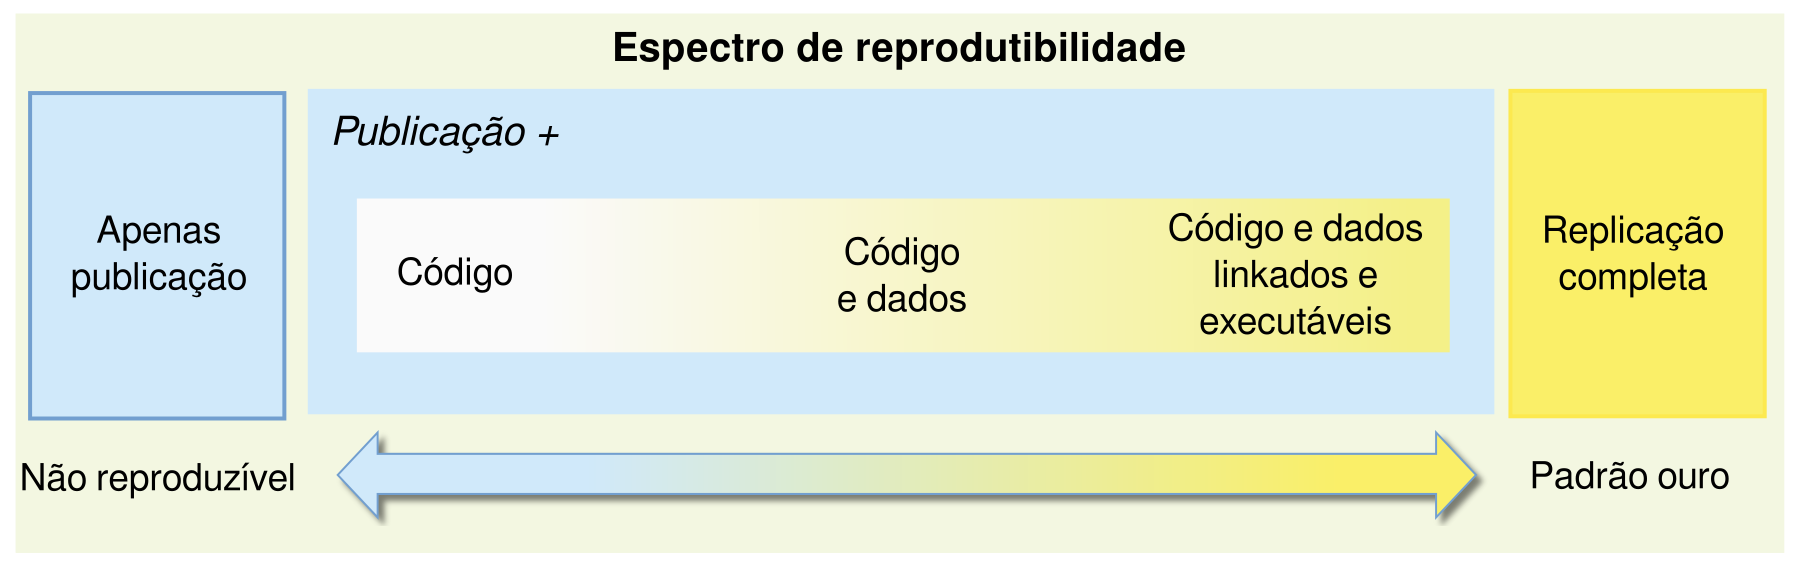
\includegraphics[scale=0.35]{imagens/reproducibility-spectrum-ptbr.png}
  \caption{Espectro de reprodutibilidade \cite{Peng2011}}
  \label{reproducibility-spectrum}
\end{figure}

Apesar das pesquisas reproduzíveis ({\it RR - Reproducible Research}) não
resolverem todos os problemas de validade experimental dos estudos em
engenharia de software, elas ao menos garantem que dados e métodos de análise
estejam disponíveis para inspeção e que os resultados possam ser derivados,
facilitando revisão logo que a publicação acontece. Além disso, é um recurso
valoroso para pesquisadores iniciantes, pesquisas reproduzíveis melhoram o
impacto do próprio estudo, por exemplo, artigos de computação que não
disponibilizam pubicamente dados e códigos possuem menos chances de serem
citados \cite{madeyski2017would}.

A disponibilidade dos softwares científicos tem sido enfatizada também em
discussões sobre sustentabilidade de software, um conceito que diz respeito
à longevidade dos sistemas de software.

%% O surgimento do conteito de engenharia de software baseada em envidências (EBSE
%% - {\it Evidence-Based Software Engineering }) surgiu em um trabalho seminal
%% apresentado em 2004 na {\it International Conference on Software Engineering
%% (ICSE)} e suas ideias e ferramentas, especialmente a revisão sistemática, tem
%% evoluído e amadurecido ao longo do tempo, e tem ajudado a caracterizar e
%% consolidar nosso conhecimento sobre muitos aspectos da pesquisa e práticas da
%% engenharia de software.
%% 
%% Em engenharia de software o termo {\it literatura} foi adicionado formando
%% revisão sistemática de literatura, isto foi feito para evitar confusão com
%% práticas de inspeção de código (comumente definido com o termo revisão) existentes
%% na área.
%% 
%% O objetivo de uma revisão sistemática é buscar e identificar todo material relevante
%% relacionado a um certo tópico (a natureza deste material é determinada pelas
%% questões de pesquisa e a natureza dos participantes intererssados na pesquisa).
%% 
%% Um fator em favor da aceitação dos conceitos da EBSE tem sido a crescente
%% reconhecimento que os resultados de estudos empíricos individuais são frequentemente
%% inconclusivos, e estes tipo de estudos são difícels de replicar com sucesso
%% \cite{sjoberg2005survey}.
%% 
%% Ainda existem poucos estudos replicados \cite{kitchenham2015evidence}.

\section{Sustentabilidade de software} \label{sustentabilidade}

% Software Sustainability: The Modern Tower of Babel

O {\it Dagstuhl Perspective Workshop} é um evento organizado por e para um
pequeno grupo de pesquisadores sêniores de renome internacional, realizado
anualmente na universidade de Dagstuhl\footnote{\url{http://www.dagstuhl.de}}
com o objetivo de refletir sobre o atual estado da ciência da computação.

Através de uma discussão intensiva com foco estratégico o workshop explora
tópicos novos e emergentes da ciência da computação produzindo manifestos que
capturam tendências e desenvolvimentos relacionados aos tópicos explorados.

Realizado desde 2011 o workshop tem explorado diversos tópicos da ciência da
computação, como computação e paleografia, tecnologia da informação como ponte
entre biologia e medicina, métodos de aprendizado de máquina para segurança de
computadores, análise de performance e visualização, entre outros tópicos. Em
sua mais recente edição, o {\it Dagstuhl Perspectives Workshop on ``Engineering
Academic Software''} \cite{allen2017engineering} examinou o estado atual dos
softwares científicos, identificou problemas comuns em seu desenvolvimento,
reconhecimento e sustentabilidade.

Uma das contribuições chave deste workshop é um manifesto contendo um roteiro
para o futuro da engenharia de software profissional e acadêmica, com foco em
instrumentos de suporte para pesquisas em software científico. O manifesto é
expresso em termos de ações ``promessas'' destinado a usuários e
desenvolvedores de softwares científicos, com passos concretos para melhorar o
ambiente em que os softwares são produzidos.

Os compromissos expressados neste manifesto são agrupados em três conceitos gerais:
(i) garantir que softwares científicos sejam {\it citados} apropriadamente;
(ii) promover a {\it carreira} do engenheiro de software desenvolvedor de software científico; e
(iii) medir a qualidade e sustentabilidade do software científico durante e após o seu {\it desenvolvimento}.

No terceiro compromisso, relacionado ao conceito {\it desenvolvimento}, o Dagstuhl Manifesto enfatiza a necessidade de medir a
qualidade e a sustentabilidade dos softwares científicos, e define
sustentabilidade de software como capacidade de perdurar, software sustentável
é aquele que continua a estar disponível no futuro, em novas plataformas e se
atende às novas necessidades \cite{allen2017engineering}.

% campos da engenharia de software, e apesar dos inúmeros entendimentos sobre o
% conceito \cite{venters2014software}, 

Essa definição de sustentabilidade de software é encontrada em mais detalhes no
{\it Karlskrona Manifesto} \cite{becker2014karlskrona}, um documento que alerta
sobre os impactos que os sistemas e a tecnologia da informação causam no futuro
do planeta, convida praticantes e pesquisadores de software a refletir sobre
o tema sustentabilidade na área da ciência da computação.

Sustentabilidade é um conceito guarda chuva composto de múltiplas dimensões, em
sua dimensão técnica, chamada sustentabilidade técnica, temos a preocupação com
a longevidade da informação, dos sistemas, e infraestrutura, e sua adequada
evolução frente as condições do ambiente em constante mudança. Software ocupa
um papel central nessa discussão, ele pode levar a crescentes consumo de
recurso, crescimento da desigualdade social, e influenciar no ganho ou perda de
auto-estima individual.

Se sustentabilidade não for levada em consideração em projetos de software, não
importa qual o domínio ou qual o propósito do software, perde-se a oportunidade
de causar mudanças positivas no planeta e na sociedade.

%Pesquisadores de
%software podem contribuir identificando questões de pesquisa em seu campo para
%ajudar a melhor entender sustentabilidade em projetos de software, Discutir com
%seus pares e pensar sobre como sustentabilidade impacta sua área de pesquisa.
%
%Assim, surge um conjunto de ações que podem ser tomadas pelos diferentes atores
%em direção à garantir sustentabilidade nos projetos de software, ações para
%praticantes de software, pesquisadores, associações profissionais, educadores,
%cientes e usuários.
% 
% 
% Em resumo os dois manifestos, Dagstuhl e Karlskrona, exprimem o conceito de
% sustentabilidade necessários para este estudo, mas é importante citar que
% algumas iniciativas e outros manifestos também estão preocupados com questões
% similares, dentre os quais podemos destacar:
% 
%A ciência aberta e comunidades de pesquisa em software tem sido bastante ativas
%em criar manifestos visando chamadas para ação. Estes manifestos chamam para melhorar
%os softwares e os metadados de bibliografia para citação persistente destes softwares.
%Outros tópicos endereçados nestes manifestos incluem ênfase no acesso ao código fonte.
%
%Agências de financiamento como o {\it US National Science Foundation} estão começando
%a reconhecer produtos de pesquisa como software assim como fazem com as publicações.
%Isto reconhece as contribuições ao softwares assim como primeiro produto de pesquisa.
%
%O {\it Journal of the American Statistical Association (JASA)} irá agora insistir na
%disponibilidade do código e dados durante a revisão dos manuscritos \cite{baker2016scientists}.
%% 
%% \begin{itemize}
%% 
%%   \item Science Code Manifesto \cite{barnes2013science}
%% 
%%     Foco em código fonte escrito especificamente para processar dados de
%%     publicações, afirma que ``todo código fonte escrito especificamente para
%%     processar dados de uma publicação deve estar disponível para os revisores e
%%     leitores do paper''.
%% 
%%   \item FORCE11 Software Citation principles \cite{smith2016software}\footnote{\url{https://www.force11.org/software-citation-principles}}
%% 
%%     Enfatiza persistencia e claridade e diz que ``Software deve ser considerado
%%     um produto legítimo de pesquisas e devem ser possível de serem citados''.
%% 
%%   \item Open Access Pledge \cite{holcombe2011openaccess}\footnote{\url{http://www.openaccesspledge.com}}
%% 
%%     Concentra-se em publicar softwares e papers em locais de {\it open access}.
%% 
%%   \item Open Science Peer Review Oath\footnote{\url{https://f1000research.com/articles/3-271/v2}}
%% 
%%     Concentra-se em potencializar os revisores para exigir acesso aberto aos
%%     softwares, práticas reprodutíveis e revisões transparentes.
%% 
%%   \item UK RSE \cite{ukrse2013}\footnote{\url{http://rse.ac.uk/who}}
%% 
%%     Conscientização sobre a importância e o papel do {\it Research Software
%%     Engineer} através de comunicação e suporta institucional.
%% 
%%   \item Reproducibility manifesto \cite{Barba2012}\footnote{\url{http://lorenabarba.com/gallery/reproducibility-pi-manifesto}}
%% 
%%     Inclui termos para fazer softwares reusáveis por outros. Foco em
%%     reprodutibilidade, deixando sustentabilidade de software fora de questão.
%% 
%%   \item The GeoScience paper of the future initiative \cite{OntoSoft2016}\footnote{\url{http://www.scientificpaperofthefuture.org/gpf/what-is-a-gpf}}
%% 
%%     Possui um conjunto de requerimentos para softwares serem incluidos em
%%     papers.  Focando mais no paper em sí do que no software.
%% 
%%   \item FAIR principles \cite{wilkinson2016fair}\footnote{\url{https://www.nature.com/articles/sdata201618}}
%% 
%%     Foco em dados de pesquisa. O objetivo é fazer eles serem encontráveis,
%%     acessíveis, interoperável e reusável. Estes princípios podem ser
%%     generalizados para aplicar aos softwares.
%% 
%% \end{itemize}

\section{Análise estática de código fonte} \label{analise-estatica}

A análise estática de código fonte é o primeiro passo para coletar informações
necessárias em diversas atividades de verificação, medição e melhoria da
qualidade de produtos de software \cite{Cruz2009, Kirkov2010}. Ela é
realizada com base no código fonte de um programa ou sistema de software, e a
partir daí descobre problemas e propriedades de sua qualidade estrutural
\cite{Chess2007}.

Ferramentas de análise estática estão disponíveis há décadas, em especial,
para programadores. A ferramenta Lint \cite{Johnson1978}, considerada a
primeira ferramenta de análise estática \cite{Gosain2015}, foi criada para
examinar programas escritos em linguagem C e aplicar regras de tipagem mais
estritas do que as regras dos próprios compiladores da linguagem.

%Neste trabalho o nosso interesse reside em compreender características de
%qualidade interna de ferramentas deste domínio de aplicação, do ponto
%de vista de desenvolvedores interessados em manter e evoluir tais ferramentas
%melhorando seus atributos de qualidade interna.
%
%A seção \ref{analise-estatica} apresenta uma definição geral da análise
%estática de código fonte, suas aplicações, sua anatomia, seus formatos de
%representação intermediária e técnicas mais comuns. 

Análise estática de código fonte tem como objetivo prover
informações acerca de um programa a partir do seu código fonte sem
necessidade de execução, e sem requerer qualquer outro artefato do programa
além do próprio código.

É um ramo que possui muitas das suas abordagens em comum com os estudos da
área de análise de programas ({\it program analysis}), especialmente na área de
compiladores, onde atua especialmente nas primeiras etapas do processo de compilação.

A análise estática de código fonte é considerada uma atividade meio com
objetivo de suportar uma variedade de tarefas comuns da engenharia de
software; muitas dessas tarefas são substancialmente úteis em atividades de
manutenção. \citeonline{Binkley2007} define uma lista dessas
atividades, incluindo:

\begin{multicols}{2}
  \begin{itemize}
    \item Análise de performance
    \item Compreensão de programas
    \item Desenvolvimento baseado em modelos
    \item Detecção de clones
    \item Evolução de software
    \item Garantia de qualidade
    \item Localizaçao de falhas
    \item Manutenção de software
    \item Recuperação arquitetural
    \item Testes
  \end{itemize}
\end{multicols}

Seja em qual atividade for, a análise estática possui importância,
pois ao ser capaz de extrair informações diretamente do
código fonte de um programa, pode auxiliar a responder perguntas necessárias
para as diversas atividades de desenvolvimento e evolução de software. Essa
importância se torna ainda mais aparente diante da ``lei'' da tendência para
execução \cite{Harman2010} que indica que todos os tipos de notação tem a
tendência de se tornar executáveis.

\subsection{Usos da análise estática de código fonte} \label{usos}

A análise de programas trata, de modo geral, da descoberta de problemas e
fatos sobre programas, ela pode ser realizada sem a necessidade de executar o
programa (análise estática) ou com informações provenientes de sua execução
(análise dinâmica).

A ideia de que programas de computador podem ser utilizados para analisar
código fonte de outros programas tem uma história de mais de 40 anos.  O
programa PFORT \cite{Ryder1974} foi projetado para localizar potenciais
problemas na portabilidade de código Fortran; em função da diversidade de
dialetos de Fortran, uma compilação sem erros não indicava que o programa
estava correto segundo os padrões da linguagem \cite{Wichmann1995}.

Desde então, ferramentas de análise estática de código fonte têm surgido para
os mais diversos fins -- muitas delas a partir das pesquisas e
desenvolvimentos da área de compiladores.  O {\it parser} utilizado nessas
ferramentas têm funcionalidades análogas aos analisadores usados em
compiladores \cite{Anderson2008}.

O uso de tais ferramentas tem se
tornado mais comum no ciclo de desenvolvimento de
software, sendo aplicadas em uma infinidade de atividades distintas visto que o
campo de aplicação destas ferramentas é bastante variado, cobrindo diferentes
objetivos. De acordo com \citeonline{Chess2007}, as atividades em que análise
estática de código fonte é empregada, destacam-se:

\begin{description}

  \item \textit{Verificação de tipos}. 
    A forma mais amplamente utilizada de análise estática, e uma das quais os
    programadores estão mais familiarizados, é a checagem de tipo.
    Previne que acidentalmente atribuam valores de forma incorreta a
    variáveis. Ainda, ao capturar erros em tempo de compilação, esta checagem
    de tipo previne erros em tempo de execução.

  \item \textit{Verificação de estilo}. 
    Os verificadores de estilo são um tipo de análise estática que aplicam regras
    de forma mais superficial do que os verificadores de tipo. São regras
    relacionadas a espaços em branco, nomes, funções depreciadas, comentários,
    estrutura do programa, entre outros. Os erros reportados por verificadores de
    estilo são aqueles que afetam a leitura e a manutenabilidade do
    código fonte, não indicando potenciais erros em tempo de execução como
    fariam os verificadores de tipo.

  \item \textit{Compreensão de programas}. 
    Ferramentas de compreensão de programa ajudam programadores a terem uma visão
    clara frente a grandes programas de computador, ou seja, programas com
    alto volume de código fonte. Ambientes de desenvolvimento integrados (IDE)
    geralmente incluem funcionalidade de compreensão, por exemplo, ``encontrar
    todos os usos de um certo método'' ou ``encontrar a declaração de uma
    variável global''. Análises mais avançadas chegam a incluir, por exemplo,
    refatoração automática. Estas ferramentas de compreensão também são úteis
    para programadores interessados em entender código fonte escrito por
    outros programadores.

  \item \textit{Verificação de programas}.
    Ferramentas de verificação de programa aceitam como entrada uma especificação
    e um conjunto de código fonte e tenta provar que o código está deacordo
    com a especificação. Quando a especificação é uma descrição completa de
    todo o programa, a ferramenta de verificação poderá realizar uma checagem
    de equivalência para garantir que o código fonte e a especificação
    combinam de forma exata. Programadores raramente têm acesso a uma
    especificação detalhada suficientemente para ser usada numa checagem de
    equivalência, o trabalho de criar esta especificação pode ser maior do que
    o trabalho de escrever o próprio código fonte do programa, desta forma
    este tipo de verificação formal raramente acontece.

  \item \textit{Localização de bugs}. 
    Um localizador de bugs está
    preocupado em apontar locais onde o programa, possivelmente, irá se
    comportar de forma inesperada. A maioria das ferramentas de localização de
    bugs são fáceis de usar porque costumam vir com um conjunto de regras
    ({\it bug idioms}) para descrição de padrões de código que indicam bugs.
    Algumas destas ferramentas costumam usar os mesmos algoritmos utilizados
    por ferramentas de verificação de propriedade.

  \item \textit{Avaliação de segurança}. 
    Ferramentas de análise estática para segurança usam as mesmas técnicas
    encontradas nas outras ferramentas, mas por ter um propósito diferente,
    identificar problemas de segurança, aplicam estas técnicas de forma diferente.
    As primeiras ferramentas de segurança (ITS4, RATS, Flawfinder) eram pouco mais
    do que um {\it ``grep''} melhorado; na maior parte, elas escaneavam o código
    procurando por funções como por exemplo {\it ``strcpy()''} que são
    facilmente usadas de forma inadequada e devem ser inspecionadas
    manualmente no processo de revisão de código fonte.

\end{description}

\subsection{Anatomia da análise de código fonte} \label{anatomia}

Ferramentas de análise estática de código fonte estão organizadas em partes ou
componentes, responsáveis por implementar três funções básicas: a) extração de dados, b) geração de representação
intermediária, e c) análise \cite{Cruz2009, Binkley2007}.

\begin{description}

  \item \textit{Extração de dados}.
    O processo de recuperar dados para futuro processamento ou armazenamento é
    chamado de extração de dados. 

    O primeiro componente da análise de código fonte é a extração de dados,
    responsável por ler o código fonte do programa e gerar uma ou mais
    representações intermediárias. Em essência, este componente converte a sintaxe
    de um programa em uma outra sintaxe abstrata e mais adequada para análise
    posterior.

  \item \textit{Representação intermediária}.
    Exportar os dados extraídos para uma representação intermediária é uma
    estratégia comum para facilitar análise e transformação de dados e
    possivelmente adição de metadados.

    Os dados obtidos na extração precisam ser representados em um formato mais
    abstrato. Esta é a responsabilidade do segundo componente da análise de
    código fonte: armazenar os dados coletados usando uma representação
    intermediária em formato mais adequado para análise automática, abstraindo
    aspectos particulares do programa e da linguagem de programação.

    Alguns tipos de representação intermediária têm sua origem na área de
    compiladores, entre os formatos mais comuns, destacam-se:

    \begin{multicols}{2}
      \begin{itemize}
        \item Árvore sintática abstrata
        \item Grafo de fluxo de controle
        \item Árvore sintática abstrata decorada
        \item Grafo de dependência de módulos
        \item Atribuição estática única
        \item Grafo de dependência de valores
      \end{itemize}
    \end{multicols}

    Estas representações podem ser utilizadas tanto na análise estática quanto
    na análise dinâmica. O uso de um ou outro formato depende do tipo de
    análise e seu propósito. Pode-se combinar diferentes tipos no sentido de
    enriquecer e estruturar a informação extraída.

  \item \textit{Análise}.
    Este componente é responsável por realizar inferências a partir dos dados
    representados internamente. O processo requer que as informações
    armazenadas estejam interconectadas e também interrelacionadas com
    conhecimento anterior. Esta análise pode gerar conhecimento quantitativo
    ou qualitativo, como, por exemplo, métricas de software ou mineração de
    dados, respectivamente. Técnicas de visualização podem ser usadas para
    apoiar este processo.

    Diversas técnicas foram desenvolvidas ao longo do tempo para realizar
    análise, algumas delas são brevemente descritas na seção \ref{tecnicas}.

\end{description}

\subsection{Formatos de representação intermediária} \label{formatos}

Essencialmente, um formato de representação intermediária é uma abstração precisa
das propriedades de um programa representado em um domínio menor. Os
compiladores normalmente constroem esta representação a fim de possuir um
modelo do programa sendo compilado, é comum que compiladores utilizem diversos
formatos durante o curso da compilação.

Em ferramentas de análise estática estes formatos são utilizados durante a
fase de análise para cumprir diversos objetivos, como por exemplo, calcular
métricas de código fonte. A métrica de complexidade ciclomática de McCabe
\cite{McCabe1976}, por exemplo, é definida com base no grafo de fluxo de controle ({\it Control Flow Graph - CFG}) do
programa com o seguinte cálculo $CC = e - n + 2p$. Onde: {\bf e} é o número de
arestas; {\bf n} é o número de nós; e {\bf p} é o número de componentes
fortemente conectados no grafo.

Assim, percebe-se que cada formato de representação intermediária pode ter fins
e objetivos bastante distintos, dentre os formatos mais comuns podemos destacar
\cite{Nielson2015, Stanier2013, Cruz2009, Ramalho1996}:

\begin{description}

  \item \textit{Árvore sintática abstrata}.
    A árvore sintática abstrata (AST - {\it Abstract Syntax Tree}) representa um
    programa tratando os elementos do código fonte como operadores e
    operandos organizados em nós numa árvore, este formato de representação é
    muito popular em tradutores {\it
    source-to-source}\footnote{http://en.wikipedia.org/wiki/Source-to-source\_compiler}.

  \item \textit{Grafo de fluxo de controle}.
    O grafo de fluxo de controle (CFG - {\it Control Flow Graph} ou {\it Call Graph}) é um grafo direcionado
    representando a estrutura de controle de um programa e sua sequência de
    instruções, onde as arestas mostram os possíveis caminhos de execução. Este
    formato é amplamente utilizado em métodos formais para otimização de
    código fonte.

  \item \textit{Grafo de fluxo de dados}.
    O grafo de fluxo de dados (DFG - {\it Data Flow Graph}) é também um grafo
    direcionado onde as arestas representam o fluxo de dados entre as
    operações do programa, este formato pode ser visto como um companheiro do
    grafo de fluxo de controle (CFG) e pode ser gerado ao longo de uma mesma
    análise.

  \item \textit{Árvore sintática abstrata decorada}.
    Árvore sintática abstrata decorada (DAST - {\it Decorated Abstract Syntax Tree}) é
    uma árvore sintática abstrata (AST) melhorada através de um processo de
    definiçao de atributos para os símbolos do programa de forma declarativa
    com uso de uma Gramática de
    Atributos\footnote{https://en.wikipedia.org/wiki/Attribute\_grammar}.

  \item \textit{Grafo de dependência de módulos}.
    O grafo de dependência de módulos (MDG - {\it Module Dependence Graph}) é um grafo
    onde os módulos são representados como nós e as arestas representam as
    relacões entre eles, indicando dependência entre os mesmos.

  \item \textit{Atribuição estática única}.
    Atribuição estática única (SSA - {\it Static Single Assignment}) pode ser vista
    como uma variação ou uma propriedade de outros formatos de representação
    intermediária, é um método que faz cada variável ser atribuída apenas uma única
    vez, facilitando a descoberta de informaçoes sobre os dados representados.

  \item \textit{Grafo de dependência de valores}.
    O grafo de dependência de valores (VDG - {\it Value Dependence Graph}) é uma
    variação que melhora (ao menos para algumas análises) os resultados
    obtidos a partir da atribuição estática única (SSA). Ele representa tanto
    o fluxo de controle quanto o fluxo de dados e assim simplifica a análise.

\end{description}

\subsection{Técnicas de análise} \label{tecnicas}

Inúmeras técnicas e métodos distintos podem ser utilizados pelas ferramentas
de análise estática, seja com o objetivo de verificação de tipos, localização
de bugs, compreensão de programas, avaliação de segurança, ou outra finalidade
qualquer. Segundo \citeonline{German2003, Li2010, Hofer2010} as técnicas e
métodos mais comumente encontrados nas ferramentas atuais são:

\begin{description}

  \item \textit{Análise léxica}.
    A análise léxica é responsável por quebrar o programa em pequenos fragmentos
    (ou {\it tokens}) e verificar se estes fragmentos são palavras válidas
    para uma dada linguagem. A análise léxica não leva em consideração a
    sintaxe do programa, sua semântica ou a interação entre módulos.

  \item \textit{Combinação de padrões de texto}.
    A combinação de padrões de texto ({\it Text-based Pattern Matching}) é a
    maneira mais simples e rápida de procurar vulnerabilidades num código
    fonte.

  \item \textit{Inferência de tipos}.
    A inferência de tipos ({\it Type inference}) refere-se a identificar o
    tipo de variáveis e funções e avaliar se o acesso a elas está em
    conformidade com as regras da linguagem. Linguagens de programação com
    sistema de tipagem incluem mecanismos deste tipo de análise.

  \item \textit{Análise de fluxo de dados}.
    A análise de fluxo de dados ({\it Data flow analysis}) resume-se a coletar
    informação semântica do código fonte do programa, e com métodos algébricos
    deduzir a definição e uso das variáveis em tempo de compilação. O objetivo
    é mostrar que nenhum caminho de execução do programa acessa uma variável
    sem definição ou atribuição prévia.

  \item \textit{Verificação de regra}.
    A verificação de regra ({\it Rule checking}) consiste em checar a segurança
    do programa através de um conjunto de regras pré-estabelecidas.

  \item \textit{Análise de restrição}.
    A análise de restrição ({\it Constraint analysis}) consiste em gerar
    e resolver restrições no processo de análise de um programa.

  \item \textit{Comparação caminho}.
    Comparação caminho ({\it Patch comparison}) inclui comparação de caminho de
    código fonte e de código-binário e é usada principalmente para encontrar
    brechas de vulnerabilidade já ``conhecidas'' e previamente divulgadas por
    fornecedores e praticantes da indústria de software.

  \item \textit{Execução simbólica}.
    A execução simbólica ({\it Symbolic execution}) é usada para representar
    as entradas de um programa através do uso de valores simbólicos ao invés
    de dados reais, produz expressões algébricas sobre a entrada dos símbolos
    do programa durante o processo de implementação e pode detectar
    possibilidade de erros.

  \item \textit{Interpretação abstrata}.
    Interpretação abstrata ({\it Abstract interpretation}) é uma descrição
    formal da análise do programa. Pelo fato de apenas controlar atributos de
    programa de preocupaçao dos usuários, a interpretação da análise semântica
    é similar ao seu significado semântico real.

  \item \textit{Prova de teoremas}.
    Prova de teoremas ({\it Theorem proving}) é baseada na análise semântica do
    programa. Converte o programa em fórmulas lógicas e então tenta provar que
    o programa é um teorema válido usando regras e axiomas.

  \item \textit{Verificação de modelo}.
    O processo de verificação de modelos ({\it Model checking}) primeiro constrói
    um modelo formal do programa tal como uma máquina de estados ou um grafo
    direcionado, então examina e compara o modelo para verificar se o sistema
    cumpre as características pré-definidas. Esta técnica requer a definição e
    descrição das propriedades que devem ser verificados por um pedaço de
    software.

  \item \textit{Verificação formal}.
    Verificação formal ({\it Formal Checking} ou {\it Compliance Analysis}) é o
    processo de provar de forma automatizada que o código do programa está
    correto em relação a uma especificação formal dos seus requisitos.

  \item \textit{Análise de fluxo da informação}.
    Análise de fluxo da informação ({\it Information Flow Analysis}) identifica
    como a execução de uma unidade de código cria dependência entre entradas e
    saídas.

  \item \textit{Verificação de sintaxe}.
    Verificação de sintaxe ({\it Syntax Checks}) tem o objetivo de encontrar
    violação de regras tais como expressões mal-formadas ou fora do padrão.

  \item \textit{Verificação de intervalo}.
    A análise de verificação de intervalo ({\it Range Checking}) tem o objetivo
    de verificar que os valores dos dados permanecem dentro de intervalos
    especificados, bem como manter a precisão especificada.

\end{description}

Diante a variedade e a constante evolução da área de análise estática
\citeonline{Novak2010} fez um estudo propondo uma taxonomia e um conjunto de
dimensões para caracterização de ferramentas de análise estática, mais detalhes
sobre essas dimensões e categorias serão exploradas no Capítulo
\ref{caracterizacao-ferramentas}, no qual apresentaremos uma caracterização de
softwares científicos estudados neste trabalho.

\section{Complexidade estrutural} \label{complexidade}

%% Métricas de software podem ser classificadas em métricas de processo, métricas
%% de projeto e métricas de produto.
%% 
%% Métricas de processo medem atributos relacionados ao ciclo de desenvolvimento
%% e manutenção de software. Métricas de projeto indicam se a execução do
%% processo está progredindo conforme planejado (por exemplo, relação entre o
%% tamanho do software entregue e o esforço total dispendido em seu
%% desenvolvimento).
%% 
%% Métricas de produto medem atributos de produtos e artefatos, como documentos,
%% diagramas, código fonte e arquivos binários. Neste trabalho,
%% apenas métricas de produto serão utilizadas.
%% 
%% Métricas de produto podem ser classificadas em internas (medem propriedades
%% visíveis apenas aos desenvolvedores) ou externas (medem propriedades visíveis
%% aos usuários) \cite{Mohamed1994}.
%% 
%% Neste trabalho, são utilizadas métricas de produto e, especificamente,
%% métricas de código fonte, que cobrem aspectos de tamanho, complexidade e
%% qualidade que podem ser medidos a partir do código fonte de um software.
%% 
%% Métricas de software tem um escopo bastante abrangente, e o termo está
%% associado com muitas atividades da engenharia de software: Medidade e modelos
%% para estimativa de custo e esforço, Coleção de dados, Modelos e medidas de
%% qualidade, Modelos de confiabilidade, Métricas de segurança, Métricas
%% estruturais e de complexidade, Avaliação de maturidade de capacidade,
%% Gerenciamento através de métricas, Avaliação de métodos e ferramentas.
%% 
%% \subsection{Métricas de código fonte} \label{metricas-de-codigo}
%% 
%% As propriedades visíveis aos desenvolvedores podem ser medidas através de
%% métricas de código fonte. A observação e o monitoramento de seus valores podem
%% indicar aspectos relevantes à manutenibilidade de um programa. Dentre as
%% inúmeras métricas de código fonte nosso interesse está em métricas que indicam
%% características relevantes à modularidade de um produto de software,
%% complexidade estrutural e custo de mudança.

%Structural and Complexity Metrics
%Desirable quality attributes like reliability and maintainability cannot be
%measured until some operational version of the code is available. Yet, we
%wish to be able to predict which parts of the software system are likely to be
%less reliable, more difficult to test, or require more maintenance than oth-
%ers, even before the system is complete. As a result, we measure structural
%attributes of representations of the software that are available in advance
%of (or without the need for) execution; then, we try to establish empiri-
%cally predictive theories to support quality assurance, quality control, and
%quality prediction. These representations include control flow graphs that
%usually model code and various unified modeling language (UML) dia-
%grams that model software designs and requirements. Structural metrics
%can involve the arrangement of program modules, for example, the use
%and properties of design patterns. These models and related metrics are
%described in Chapter 9.

Do ponto de vista de métricas, neste trabalho, estamos interessados, de fato, na métrica
de complexidade estrutural SC ({\it Structural Complexity}), uma medida da
complexidade de projetos de sistema de software proposta por
\citeonline{Darcy2005} como indicador da complexidade dos sistemas de software
em relação à sua estrutura interna e ao relacionamento entre os seus
componentes.

Complexidade é um tema bastante amplo, e para compreender onde os
sistemas de softwares se encaixam neste contexto precisamos definir brevemente
o que vem a ser sistemas complexos.

Sistemas complexos são sistemas no qual grandes redes de componentes sem
controle central dão origem a um comportamento
coletivo complexo, com processamento sofisticado de informação, e adaptação
através de aprendizado ou evolução \cite{Mitchell2009}. As seguintes
características são comuns a todos os sistemas complexos:

\begin{description}

  \item[Comportamento coletivo complexo.] Apesar de serem compostos por
  elementos bastante simples individualmente, sistemas complexos podem exibir
  comportamentos coletivos bastante sofisticados.

  \item[Troca de sinais e processamento de informação.] Em cada um destes
  sistemas, seus componentes individuais consomem e produzem informação entre
  si. Parte do comportamento do sistema envolve transformação dessa informação.

  \item[Adaptação.] Sistemas complexos adaptam-se a novas situações de forma a
  aumentar suas chances de sobrevivência diante de novas condições em seu
  ambiente.

\end{description}

Os sistemas complexos podem ser classificados como naturais ou artificiais, os
sistemas naturais são aqueles cuja constituição não tem participação humana, ao
contrário dos sistemas artificiais que são projetados por humanos, com
objetivos e funções previamente definidos \cite{Simon1996}. Neste sentido,
sistemas de software podem ser caracterizados como sistemas complexos
artificiais, pois exibem comportamento coletivo complexo, realizam trocas de
sinais e processamento de informação e passam por adaptação para se adequar a
mudanças em seu ambiente.

Sistemas de software são compostos por componentes, em geral, chamados de
módulos, que possuem tanto estado quanto comportamento próprios,
módulos individuais de um sistema de software são simples quando comparados com
o sistema como um todo. Módulos produzem informação para outros módulos
através de parâmetros em chamadas de sub-rotinas e consomem informação através
dos valores de retornos destas chamadas. O fluxo contínuo de novos requisitos e
de mudanças no ambiente operacional de sistemas de software força-os a se
manter em constante evolução em busca de “sobrevivência”.

Esta medida é, possivelmente, um indicativo de problemas na manutenibilidade de
sistemas de software, em especial sobre o esforço necessário para atividades de
manutenção \cite{Terceiro2012}. Ela está relacionada a como os módulos de um
programa estão organizados bem como à estrutura interna de cada módulo. Esta
métrica pode dar indícios importantes sobre características arquiteturais de um
programa de software e pode explicar seus atributos de qualidade interna.

%Modularity
%Modularity describes the logical partitioning of software into several parts, components, and modules.
%Software will be easy to understand and change when composed of independent modules.
%“A Software Maintainability Evaluation Methodology”, 1981
%\cite{kumar2012survey}

%Faz um experimento usando CBO LCOM e outras metricas como preditor de manutenabilidade...
%\cite{Dagpinar2003}

%A complexidade de um sistema de software pode ser de três tipos: a complexidade
%do problema, a complexidade procedural, e a complexidade do projeto do sistema.
%Esta última é o foco deste trabalho.
%A complexidade do problema está relacionada ao domínio do problema.
%A complexidade procedural está relacionada à estrutura lógica da programa, em es-
%pecial do seu comprimento, em termos de número de tokens, linhas de código fonte, ou
%estruturas de controle. Este último tipo é o que iremos estudar neste trabalho.
%
%Os sistemas complexos podem naturais ou artificiais, uma colônia de formigas
%por exemplo pode ser caracterizado como um sistema complexo natural, onde
%individualmente cada formiga se apresenta como criatura relativamente simples,
%com instintos básicos como procurar alimento, responder a estímulos químicos
%vindos de outras formigas, combater intrusos, etc. No entanto, quando
%observadas coletivamente em uma colônia, as formigas aparentam ser muito mais
%sofisticadas. Elas são capazes de se organizar em diferentes atividades, criar
%estruturas complexas dentro de seu formigueiro, e de encontrar o caminho mais
%curto para uma fonte de alimento.
%
%Os sistemas naturais são aqueles cuja constituição não tem participação humana.
%Sistemas artificiais são projetados por humanos, com objetivos e funções
%definidos.  Sistemas artificiais podem ou não serem projetados à imagem de um
%sistema natural, e durante a sua concepção eles são discutidos em termos tanto
%de suas características (o que eles são) como de necessidades que eles devem
%satisfazer (o que eles deveriam ser) \cite{Simon1996}.
%
%É importante ressaltar que esta caracterização de sistemas de software como
%sistemas complexos diz respeito à estrutura interna dos sistemas, ou seja, aos
%componentes que o constituem e ao relacionamento entre estes componentes. Não
%foram considerados outros aspectos importantes de sistemas complexos, como por
%exemplo o seu relacionamento com o ambiente externo.
%
%como uma combinação das métricas de acoplamento (CBO) e coesão (LCOM4), 
%
%Sistemas de software, no entanto, se
%diferenciam dos sistemas complexos naturais pelo fato de serem projetados;
%consequentemente, o seu processo evolucionário não é intrinsecamente parte do
%seu comportamento, mas fruto da ação consciente de seus desenvolvedores.
%
%\cite{Tegarden1995}
%
%"The implication of this result is that, when
%designing, implementing, and maintaining software to control complexity, both coupling and cohesion should be considered jointly,
%instead of independently" Darcy 2005
%
%Many studies have demonstrated a significant correlation between
%LOC and the cyclomatic number. The researchers usually suggest that
%this correlation proves that cyclomatic number increases with size; that
%is, larger code is more complex code. However, careful interpretation of
%the measures and their association reveals only that the number of deci-
%sions increases with code length, a far less profound conclusion. The cyclo-
%matic number may be just another size measure. Chapter 9 contains more
%detailed discussion of validation for the McCabe measures.
%
%{\bf SC} {\it Structural Complexity (Complexidade estrutural)}: mede a
%complexidade do software \cite{Darcy2005} combinando os valores de CBO e LCOM4.

\citeonline{Darcy2005} definem complexidade estrutural como uma combinação de
acoplamento e coesão. Estes são dois conceitos complementares: enquanto o
acoplamento reflete o relacionamento entre módulos, a coesão nos fornece uma
visão da organização dos componentes internos de um módulo e seus
relacionamentos.

Uma formalização da métrica proposta por \citeonline{Darcy2005} pode ser
expressa da seguinte maneira, para um projeto $p$ e seu conjunto de módulos
$M(p)$, a complexidade estrutural $SC(p)$ de $p$ é:

\begin{equation}
SC(p) = \frac
{ \displaystyle \sum_{m \in M(p)} CBO(m) \times LCOM4(m) }
{ |M(p)| }
\end{equation}

Esta medida de complexidade estrutural é portanto a complexidade
estrutural média entre todos os módulos do sistema.

\begin{itemize}

  \item {\bf CBO} {\it Coupling Between Objects (Acoplamento entre objetos)}:
    mede o acoplamento entre objetos do software \cite{Chidamber1994}
    calculando em nível de classe o número total de acessos à outras classes do
    mesmo sistema, é comum ser também chamada de Fan-out da classe. CBO é então
    definida pela seguinte fórmula:

\begin{equation}
\label{formula-cbo}
CBO(C) = \sum_{i=1}^{n} cliente(C, Ci)
\end{equation}

Onde:

\begin{equation}
cliente(Ci, Cj) =
  \begin{cases}
    1 \text{ se } Ci \Rightarrow Cj \wedge Ci \neq Cj \\
    0 \text{ caso contrario} \\
  \end{cases}
\end{equation}

A notação $ Ci \Rightarrow Cj $ indica acesso à atributos, variáveis, métodos ou funções
entre módulos ou classes.

Apesar de ser possível formalizar a métrica CBO através da fórmula acima, sua descriçao original é
bastante complexa, levando à implementações variadas do seu cálculo
\cite{Lincke2008}. A definição original, por exemplo, inclui explicitamente
acoplamento via herança \cite{Harrison1998}, no entando não deixa claro como
deve ser tratado métodos herdados \cite{Briand1999}. A definição original
afirma também que apenas chamadas explícitas (e não chamadas implicitas) de
construtores são contabilizadas. Algumas definições de CBO incluem não apenas $
cliente(Ci, Cj) $ mas também a recíproca $ cliente(Cj, Ci) $ de forma que o valor
final inclui classes que ela acessa somado ao número de classes do sistema que
a acessam \cite{Sant2008}.

Quanto mais as classes forem independentes, mais fácil é reutilizá-las e menos
arriscado é modificá-las. Classes mais acopladas precisam de mais rigor em
testes, pois mais partes do sistema dependem delas.

  \item {\bf LCOM4} {\it Lack of Cohesion in Methods (Ausência de coesão em
    métodos)}: mede o grau de falta de coesão em métodos \cite{Hitz1995}.

O cálculo de LCOM4 é dado através de grafo não-orientado em que os nós ou
vértices são os métodos e atributos de uma classe e as arestas são acessos à
métodos e atributos. O cálculo desta métrica pode ser formalizado como a
seguir \cite{Silva2012}.

Seja $ X $ uma classe qualquer e $ M_x $ o conjunto de métodos desta classe,
considere um grafo simples não-orientado $ G_x(V, E) $, sendo:

\begin{equation}
V = M_x
\text{ e }
E = \{ \langle m, n \rangle \in V \times V \}
\end{equation}

Onde:
\begin{equation}
(\exists i \in Ix : (m \text{ accessos } i) \land (n \text{ accessos } i)) \lor (m \text{ chamadas } n) \lor (n \text{ chamadas } m)
\end{equation}

O valor da métrica LCOM4 para uma classe $ X $ é então definido como o número
de componentes conectados do grafo $ G_x (1 \leq LCOM(x) \geq | M_x |)$.

Coesão entre os métodos de uma classe é uma propriedade desejável, portanto o
valor ideal para esta métrica é 1. Se uma classe tem diferentes conjuntos de
métodos não relacionados entre si, é um indício de que a classe deveria ser
refatorada em classes menores e mais coesas.

\end{itemize}
                         % related work

%------------------------------------------%

\xchapter{Método de pesquisa}
{Este capítulo apresenta a metodologia utilizada para coleta e análise dos
dados do ecossistema de software acadêmico de análise estática}
\label{metodologia}

%Lembrar de destacar o contexto (ASE, SCAM, etc.)
Este trabalho apresenta um estudo de caso exploratório ({\it exploratory case
study}) \cite{stol2015holistic} sobre a sustentabilidade do ecossistema de
software acadêmico de análise estática.
% exploratória ou descritiva? exploratória

% Decidir se será HIPOTESE geral ou QUESTAO DE PESQUISA principal.
Hipótese geral: o atual modelo de desenvolvimento de software do ecossistema de
software acadêmico de análise estática é insustentável.

% Q1: O ecossistema de software acadêmico de análise estática sofre %sérios problemas de sustentabilidade?
% Q2: Quais os tipos de problema?
% Q3: ...

% compartilhamento é um requisito para colaboração
% disponibilidade é um requisito para colaboração
% licenças expressas previamente são requisitos para colaboração
% visibilidade do software é requisito para colaboração
% preocupação com sustentabilidade e qualidade dos produtos é requisito para colaboração

%%%%%%%%%%%%%%%%%%%%%%%%%%%%%%%%%%%%%%%%%%%%%%%%%%%

%No segundo estudo, os softwares com código fonte disponível foram avaliados em
%relação a sua manutenabilidade através da métrica de complexidade estrutural. A
%coleta dessa métrica para cada software foi realizada pelo Analizo, uma suíte
%de ferramentas para análise de código fonte, e está sendo considerado como um
%indicador de manutenabilidade.

%Um conjunto de softwares de análise estática da indústria foi incluído nesta
%etapa, todos os dados coletados para os softwares acadêmicos foram também
%coletados para este novo conjunto. Esses softwares foram então caracterizados em
%relação à frequencia de lançamentos, linguagem de programação e o tipo de
%entrada suportado.

%Questão de pesquisa:

%* Como ocorre o co-desenvolvimento dos softwares
%* Como acontece colaboração na construção dos softwares
%* Como os softwares contribuem para a construcao de conhecimento novo em novas pesquisas derivadas

% * mais da metade desenvolvem seus próprios softwares
% * falta de visibilidade gera questionamentos sobre qualidade
% * falta de treinamento leva a produzir softwares sem qualidade
% * produtividade científica requer capacidade de replicação
% * capacidade de replicação depende de qualidade

%(mover os coding schema para anexos ou (nao) e manter todos os campos incluindo os de howison
%e os meus, em cada etapa vou preenchendo mais dados, na seleção estruturada pego o mínimo,
%na próxima coleta preencho com mais questões, criador, etc)

%será
%aplicado automaticamente com auxílio de um script desenvolvido durante este
%trabalho de pesquisa, detalhes deste script, outros artefatos produzidos
%durante esta pesquisa, e onde obtê-los pode ser encontrado no Apêndice
%\ref{reproducibilidade-do-estudo}.

%\begin{verbatim}
%  "tool" OU "framework"; E
%  "download" OU "available"; E
%  "http" OU "ftp"; E
%  "static analysis" OU "parser".
%\end{verbatim}

%As informações coletadas sobre cada software inclui nome, descrição e o
%endereço onde obter uma cópia, normalmente página web ou repositório de código
%fonte, esses endereços foram verificados para confirmar se os softwares estão,
%de fato, disponíveis.

%segundo as definições de software {\it
%livre} e {\it open} da Free Software
%Foundation\footnote{\url{https://www.gnu.org/philosophy/free-sw.html}} e Open
%Source Initiative\footnote{\url{https://opensource.org/osd}}, respectivamente,

%#### artigos nao encontrados para download:
%
%  url = {http://doi.acm.org/10.1145/3090064.3090070},

% * revisão estruturada
%    paper{step} = 'structured-review';
% * citações ao software
%    citations{key}{step} = 'review-citations';

% contribuições sem peso:
% =======================
% o software mudou de nome, qual o nome antigo, qual o novo nome
% um novo software foi criado a partir daqui, qual o nome do novo
% um novo software foi criado com base neste

%O antipositivismo, por outro lado, postula que toda a verdade é construída
%socialmente, o que significa que os seres humanos criam sua própria verdade
%sobre as questões de relevância para elas e essas verdades socialmente
%construídas são válidas e valiosas.

%as próprias pessoas, introduzem aspectos que são especialmente difíceis de capturar.
%Entretando, estudos tentando capturar comportamento
%humano como isto se relaciona ao engenharia de software tem aumentado e, não
%surpreendentemente, estão aumentando o uso empregando de métodos qualitativos

%O pesquisador positivista vê a verdade objetiva quanto possível, ou seja,
%existe alguma verdade absoluta sobre as questões de relevância, mesmo que essa
%verdade seja evasiva e que o papel da pesquisa seja cada vez mais próximo
%disso.

%O estudo de engenharia de software tem sido complexo e difícil. A complexidade
%surge de questões técnicas, do desastrada intersecção entre máquina as
%capacidades (ou qualidades?) humanas e de máquina, e do papel central que
%pessoas tem na realização de tarefas da engenharia de software.

%Os primeitos dois aspectos oferecem mais do que apenas problemas complexos para
%manter os pesquisadores de engenharia de software empírica ocupados. Mas o
%último fator, as próprias pessoas, introduzem aspectos que são especial,ente
%difíceis de capturar. Entretando, estudos tentando capturar comportamento
%humano como isto se relaciona ao engenharia de software tem aumentado e, não
%surpreendentemente, estão aumentando o uso empregando de métodos qualitativos

%Veja Creswell (1998) para uma explicação
%mais completa do positivismo, do interpretivismo, de outros quadros filosóficos
%relacionados e do papel dos métodos de pesquisa qualitativa neles.
%   weightless\_contributions={},

%Os métodos qualitativos são apropriados para (mesmo, implicitamente) pesquisa
%positivista em engenharia de software, e um pesquisador não precisa se
%inscrever de todo o coração para a visão de mundo interpretativa
%(antipositivista) para aplicá-los.

%Os dados qualitativos são dados representados como texto e imagens, não números (Gilgun, 1992).

%O foco deste capítulo é bastante estreito, na medida em que se concentra em
%apenas algumas técnicas, e apenas alguns dos possíveis projetos de pesquisa que estão bem
%adequado para tópicos comuns de pesquisa em engenharia de software. Veja Judd et al. (1991),
%Lincoln e Guba (1985), Miles e Huberman (1994) e Taylor e Bogdan
%(1984) para descrições de outros métodos qualitativos.

%A apresentação deste capítulo divide métodos qualitativos para aqueles para
%coletando dados e aqueles para análise de dados. Exemplos de vários métodos são fornecidos
%para cada um, e os métodos podem ser combinados entre si, bem como com
%métodos quantitativos.

%Ao longo deste capítulo, serão extraídos exemplos de
%vários estudos de engenharia de software, incluindo (von Mayrhauser e Vans 1996;
%Guindon et al., 1987; Lethbridge et al., 2005; Perry et al. 1994; Lutters and Seaman,
%2007; Singer, 1998; Orlikowski 1993).

%Exemplos mais detalhados também serão usados
%de estudos descritos em Parra et al. (1997) e Seaman e Basili (1998) porque
%eles representam a experiência do autor (tanto positiva como negativa).

%A Computação muitas vezes é vista como uma disciplina de
%engenharia. Existe a engenharia de software, a engenharia de
%computação e a engenharia de computadores, cada qual com
%um objetivo diferenciado, mas sendo que todas têm em
%comum a produção de conhecimento para aplicação em
%processos de produção de software, sistemas ou hardware.

%A ciência aplicada muitas vezes é confundida com a
%tecnologia. Mas, como será visto adiante, são coisas distintas.

%A perspectiva crítica entende o mundo como a construção histórica e social
%de relações de poder e dominação. Nesta visão sistemas de informação pro-
%vavelmente herdam da sociedade relações de poder, alienação e dominação,
%e revelar essas heranças é o objetivo central da pesquisa qualitativa de fundo
%crítico. [Myers and Young. 1997] é um bom exemplo de pesquisa qualitativa de
%fundo crítico em CC.

%Para muitos pesquisadores de ciências sociais, os métodos qualitativos são
%reservados exclusivamente para uso de pesquisadores antipositivistas e não devem
%ser misturados com métodos quantitativos ou pontos de vista positivistas.

%Os métodos de pesquisa qualitativa foram projetados,
%principalmente por pesquisadores educacionais e outros cientistas sociais
%(Taylor e Bogdan, 1984), para estudar as complexidades de humanos (por exemplo,
%motivação, comunicação, compreensão).


%Numa primeira definição, métodos qualitativos diferem de métodos quanti-
%tativos porque se ocupam de variáveis que não podem ser medidas, apenas
%observadas. Essa é uma dicotomia muito simplista. Métodos qualitativos vêm
%das ciências sociais, em oposição aos métodos quantitativos que derivam das
%ciências naturais.

%Essa diferença na origem já é suficiente para que visões
%diferentes sobre o que é ciência, e como se faz ciência, tornem definições sus-
%cintas sobre o que é um ou outro método muito difícil.


%surgiram de um 
%Historicamente, os métodos de pesquisa qualitativos surgiram da tradição
%interpretativa, ou antipositivista, na pesquisa em ciências sociais.
%O antipositivismo, por sua vez, surgiu como uma reação ao positivismo, que foi
%e continua a ser o fundamento filosófico prevalecente (implícito) da pesquisa
%em ciências naturais e físicas, incluindo a ciência da computação e a
%engenharia de software.

%se presta a combinar recursos qualitativos e métodos quantitativos, a fim de
%aproveitar os pontos fortes de ambos.

%pelo encontro de qualidades
%humanas e de máquinas, e o papel central que as pessoas desempenham nas tarefas
%da engenharia de software. Os aspectos humanos são especialmente difíceis de
%capturar e tem chamado atenção e atraído métodos de pesquisa e coletada de
%dados tradicionais de outros campos, especialmente, das ciências sociais.
%
%ciencias formais: logica e matematica, na computação: teoria dos algoritmos, linguagens formais, autômatos
%ciencias empiricas:
%  ciencias naturais: astronomia, fisica, quimica, na computação: eletronica, circuito logicos
%  ciencias sociais: historia, psicologia, sociologia, na computação: informatica na educação, comércio eletrônico, games, IHC
%
%ciencias puras: formal (lógica) ou empírica (cosmologia), na computação: pouca atuação e presença da computação ainda
%ciencias aplicadas: engenharias, na computação: engenharia de software, informatica na educação, etc
%
%ciencias exatas: matemática, física, química, na computação: a computação é uma ciência exata, a princípio
%ciencias inexatas: metereologia, economia, maioria ciencias sociais, na computação: algoritmos geneticos, casos de redes neurais
%
%ciencias duras: rigor cientifico em observações, experimentos, etc
%  ciencias duras formais: muito uso de logica e matematica
%  ciencias duras naturais: costumam depender de estatistica, exige rigor na comprovação de resultados empiricos, medicina
%
%ciencias moles: aceitam evidencias via estudos de caso por exemplo
%
%ciencias duras X ciencias moles, computação: normalmente entende-se computação como ciência dura, mas ainda
%                                             existe dificuldade de providenciar dados ....
%
%


%Contrário a fontes como [Myers 1997], que classifica a pesquisa qualitativa
%em 4 grupos, eu acho a divisão em apenas dois grupos mais produtiva: a
%pesquisa observacional e a pesquisa-ação (action research).

%A pesquisa
%observacional tem como objetivo observar o ambiente, mas não modificá-lo; já
%o objetivo central da pesquisa-ação é modificar o ambiente.

%É claro que só a
%presença do pesquisador causa alguma modificação no ambiente, mas essa
%modificação não é o objetivo da pesquisa observacional, e algumas variantes
%da pesquisa observacional tentam eliminar esse efeito.

%Segundo vários autores (por exemplo [Orlikowski and Baroudi 1991]) a pes-
%quisa qualitativa onservacional pode ser dividida segundo a perspectiva filosó-
%fica ou epistemológica que a embasa em:
%
%positivista
%interpretativista
%crítica
%
%Eles também são usados para responder o "porquê" às perguntas já
%abordadas pela pesquisa quantitativa.

%Normalmente entende-se a Computação como uma ciência
%dura, mas a realidade ainda, em muitos casos é que os
%pesquisadores têm dificuldade em providenciar dados em
%quantidade suficiente para dar suporte empírico a suas
%conclusões. Assim é que se vêem ainda muitos artigos em
%Computação que utilizam um ou alguns poucos estudos de
%caso para tentar “validar” uma técnica, modelo ou teoria.
%Como visto adiante, o estudo de caso é uma excelente fonte de
%dados para uma pesquisa exploratória, mas, a não ser no caso
%de contradição de uma teoria comumente aceita, o estudo de
%caso não valida a hipótese em estudo.

%Embora a posição filosófica implícita predominante dessas áreas
%de pesquisa permaneça positivista.
%Historicamente os métodos de pesquisa da ciência
%da computação e engenharia de software se fundamentam em filosofias opostas
%ao que fizeram surgir os métodos qualitativos, assim como as ciências naturais
%e físicas.

%Os métodos são descritos aqui em termos de como eles poderiam ser usados em um estudo que
%mistura métodos qualitativos e quantitativos, como muitas vezes são em estudos de software
%Engenharia.

%Eles ajudam a responder perguntas que envolvem variáveis difíceis
%de quantificar (particularmente a característica humana como
%motivação, percepção e experiência).

%outros campos, especialmente, das ciências sociais.
%Métodos qualitativos, então, foram necessários para capturar e descrever essas
%realidades socialmente construídas.

%Há desvantagens no
%entanto.  A análise qualitativa é geralmente mais intensiva em mão-de-obra em
%comparação com análise quantitativa. Os resultados qualitativos geralmente são
%considerados "mais suaves/leves" ou "Mais confusos/fuzzier" do que resultados
%quantitativos, especialmente em comunidades técnicas como a nossa.  Eles são
%também mais difíceis de resumir ou simplificar.

%A principal vantagem da pesquisa bibliográfica reside no fato de permitir ao
%investigador a cobertura de uma gama de fenômenos muito mais ampla do que
%aquela que poderia pesquisar diretamente

%A pesquisa bibliográfica também é indispensável nos estudos históricos

%Enquanto a pesquisa bibliográfica se utiliza fundamentalmente das contribuições
%dos diversos autores sobre determinado assunto, a pesquis"ã documental yale-se
%de materiais que não recebem ainda um tratamento analítico, ou que ainda podem
%ser reelaborados de acordo com os objetos da pesquisa

%A pesquisa bibliográfica é desenvolvida com base em material já elaborado,
%constituído principalmente de livros e artigos científicos

%Uma vantagem da pesquisa documental é que os documentos constituem fonte rica e
%estável de dados

%Outra vantagem da pesquisa documental está em seu custo

%Outra vantagem da pesquisa documental é não exigir contato com os sujeitos da
%pesquisa

%\cite{wazlawick2015metodologia}

%por exemplo, em pesquisadores em sistemas de
%informação, interação homem-computador e engenharia de software.
%emprestado a experiência acumulada dos cientistas sociais aplicadas no contexto
%da computação, 

%De um modo geral, métodos qualitativos em ciência da computaçao são métodos que
%se caracterizam por ser um estudo aprofundado de um sistema no ambiente onde
%ele está sendo usado, ou, em alguns casos, onde se espera que o sistema seja
%usado. Métodos qualitativos sempre envolvem pessoas, e na maioria das vezes
%sistemas.

%A metodologia adotada neste estudo para a coleta de dados é do tipo: A técnica
%de coleta de dados utilizada neste trabalho é a Consulta Documental a materiais
%escritos de diferentes tipos dos registros ....  ; manuais, relatórios e outros

%3.3. Independent Techniques
%       3.3.1. Analysis of Electronic Databases of Work Performed
%       3.3.2. Analysis of Tool Logs
%       3.3.3. Documentation Analysis
%       3.3.4. Static and Dynamic Analysis of a System
%4.2. Coding and Analyzing the Data
%\cite{singer2008software}

%Estudos em engenharia de software descrevemos uma série de técnicas de coleta
%de dados para esses estudos, organizados em torno de uma taxonomia com base no
%grau em que a interação com engenheiros de software é necessária.

%mas pouco se sabe sobre como os engenheiros de software realizam seu
%trabalho. Para melhorar as ferramentas e a prática de engenharia de software,

%A principal vantagem de usar métodos qualitativos é que eles forçam a
%pesquisador para investigar a complexidade do problema em vez de abstrai-lo.
%Assim, os resultados são mais ricos e mais informativos. Técnicas
%independentes, ou seja, são técnicas caracterizadas pela ausencia da
%necessidade de interação entre pesquisador e com os atores sendo estudados.

%, sendo marcada por
%aspectos comportamentais humanos, 
%bastante

%essencialmente por
%questões humanas e de máquinas, e o papel que as pessoas desempenham nas
%tarefas da prática em engenharia de software, os aspectos humanos são
%especialmente difíceis de capturar e tem atraído a atenção dos cientistas para
%métodos de pesquisa pouco usuais, tanto em estudos da ciência da computação,
%quanto da engenharia de software.

%se presta a
%combinar métodos qualitativos e quantitativos, a fim de aproveitar os pontos
%fortes de ambos. A pesquisa de engenharia de software tem sido bastante
%atrasada para reconhecer o valor dos estudos qualitativos. Esta atenção tem
%sido notada nas últimas décadas, por exemplo, através da adoção de métodos
%qualitativos, especialmente em estudos de campo voltados para estudar
%profissionais reais à medida que resolver problemas reais.

%estudo de campo, com coleta de dados através de pesquisa documental

%\cite{brooks2008replication}
%\cite{wainer2007metodos}
%\cite{singer2008software}
%\cite{wazlawick2015metodologia}

%A engenharia de software, apesar de ser uma atividade marcada fortemente por
%aspectos técnicos e humanos, tem sido lenta em reconhecer o valor do método de
%pesquisa qualitativo e seu alto potencial para investigar a complexidade de
%problemas reais sem necessidade de abstrai-los, fonecendo resultados ricos e
%informativos, especialmente sobre questões relacionadas a crenças,
%experiências, atitudes e opiniões de indivíduos ou grupos
%\cite{seaman1999qualitative}.

%, com as seguintes características
%principais:

%estratégia de pesquisa: trabalho de campo
%método de pesquisa: exploratory case study,

%Adotamos uma estratégia de pesquisa de trabalho de campo (Field Studies),
%segundo o framework apresentado em \citeonline{stol2015holistic}, de
%configuração natural (Natural Settings),

%novos conhecimentos e uma compreensão mais profunda dos fenômenos investigados
%* without any intervention by the researchers.
%* focuses on a particular phenomenon, organization or system
%* level of generalizability to a large population is much lower (due to the specific context)
%* to study software professionals or software systems
%* do not include any deliberate modification of the environment in which the research is conducted
%* having a low level of precision of measurement or control as would be found in laboratory experiments
% \item conduzida numa configuração de mundo real
% \item máximo no realismo do contexto
%Maximizes realism of context
%Low on precision of measurement
%Low on generalizability of results

%\begin{itemize}
%  \item Com o foco num fenômeno, organização ou sistema em particupar
%  \item Com um baixo nível de generalização e alto realismo do contexto
%  \item Sem intervenção do pesquisador no ambiente
%\end{itemize}

%STRATEGIES:
%
% * I    Field Studies +‘maximum’ in realism of context
% * I    Field Experiments
%
% * II   Experimental Simulations
% * II   Laboratory Experiments
%
% * III  Judgment Tasks
% * III  Sample Surveys
%
% * IV   Formal Theory
% * IV   Computer Simulations

%duas dimensões principais: obtrusiveness e generality
%                           ‘intrusion’

%As configurações em que as estratégias de pesquisa são adotadas variam,
%four different types of research settings; I, II, III, IV

%I     Natural Settings
%      * the researcher has no goal to make any changes or control any variables of interest
%      * intrusao em Field Experiments é maior que em Field Studies

%II    Contrived Settings
%      * artificially created by a researcher for the sole purpose of the study
%      * top of the ‘obtrusiveness’, maior controle que Field Experiment, Laboratory Experiments tem o maximo de controle

%III   Setting-Independent
%      * aim to gather observations of behavior (people, systems) that is independent from the setting
%      * Judgment Tasks are used to elicit responses from a set experts, or judges about a certain topic
%      * Sample Surveys aim to gather data from a larger group of respondents and as such usually have a better generalizability

%IV    No Empirical Setting
%      * are not empirical strategies but rather are theoretical.

%The choice of research strategy, ‘big picture’

%(( Runkel and McGrath derived a framework to position different research strategies [29] \cite{runkel1972research} ))

%A ``estratégia de pesquisa'' tem um impacto significativo sobre o que pode e
%não pode ser alcançado em um estudo em termos de aquisição de novos
%conhecimentos e uma compreensão mais profunda dos fenômenos investigados
%\cite{stol2015holistic}.

%Utilizamos como estratégia de 
%\cite{seaman1999qualitative}.

%Exemplos de
%seus resultados são o código-fonte, a documentação e os relatórios. Os
%subprodutos são criados no processo de trabalho, por exemplo, solicitações de
%trabalho, trocas de logs e saída do gerenciamento de configuração e ferramentas
%de compilação. Esses repositórios ou arquivos podem servir como fonte primária
%de informações.

%Este trabalho apresenta uma pesquisa exploratória, do tipo documental, com o
%objetivo principal de aprimorar o conhecimento a respeito da sustentabilidade
%do ecossistema de software acadêmico de análise estática.
                           % setup

%------------------------------------------%

\xchapter{Avaliação da sustentabilidade técnica dos softwares acadêmicos de análise estática}
{Este capítulo apresenta a avaliação dos softwares acadêmicos de análise
estática de código fonte quanto à sua sustentabilidade técnica, ou seja, a
capacidade de perdurar, de continuar disponível no futuro.}
\label{sustentabilidade-tecnica}

% Introduction
% Background
% Experimental Setup (hipoteses / design)
% Results (data analysis)
% Discussion
% Threats to validity
% Conclusions

% Muitos estudos em engenharia de software sofrem de dificuldades de repetição
% \cite{Tang2016}, artigos citando desenvolvimento de scripts ou protótipos
% apresentam chance próximo a nulo de terem tais artefatos disponíveis, a
% replicabilidade das pesquisas tendem a cair com a idade da publicação, páginas
% ou repositórios se tornam indisponíveis com o passar do tempo
% \cite{robles2010replicating}, não se sabe como as taxas de softwares
% disponíveis, executáveis, e escondidos ({\it hidden software}) mudam ao longo
% do tempo \cite{allen2017engineering}, softwares acadêmicos são, muitas vezes, mal
% documentados, não intuitivos e difíceis de instalar, uma fração substancial são
% abandonware, ou seja, não são mais mantidos ou desenvolvidos ativamente, mesmo
% tendo um valor potencial para a comunidade científica \cite{list2017ten}.
%
%apesar disso, antes mesmo de resolver tais questões é
%fundamental compreender os impactos que eles causam na comunidade de pesquisa.

Este estudo tem como objetivo medir e avaliar a sustentabilidade técnica dos
softwares acadêmicos de análise estática publicados na literatura acadêmica.

%Estes são alguns problemas relacionados aos softwares acadêmicos, muitos são
%resultado de baixos orçamentos, limitação de tempo e alta rotatividade entre os
%grupos de pesquisa, outros são, possivelmente, ocasionados por questões
%culturais \cite{niemeyer2017open}, como, por exemplo, a tímida adoção de
%práticas da ciência aberta entre pesquisadores. Compreender os reais motivos
%por trás destes problemas seria, naturalmente, o passo essencial para solucioná-los,
%apesar disso, antes mesmo de resolver tais questões é
%fundamental compreender os impactos que eles causam na comunidade de pesquisa.

\section{Planejamento do estudo}

\subsection{Questões de pesquisa}

Neste estudo as seguintes questões de pesquisa serão investigadas:

\newcommand{\QuestaoUm}{Na literatura científica publicada, como as taxas de
softwares publicados, no domínio de aplicação de análise estática, mudam ao
longo do tempo?}

\newcommand{\QuestaoDois}{Os softwares acadêmicos de análise estática, publicados
na literatura científica, estão disponíveis para obtenção hoje?}

\newcommand{\QuestaoTres}{Na literatura científica publicada, como as taxas de
softwares disponíveis, no domínio de aplicação de análise estática, mudam ao
longo do tempo?}

\newcommand{\QuestaoQuatro}{Podemos adaptar de forma incremental os softwares
acadêmicos de análise estática para aproveitar oportunidades emergentes, sem
perda de reprodutibilidade?}

\begin{description}
  \item [Q1:] \QuestaoUm
  \item [Q2:] \QuestaoDois
  \item [Q3:] \QuestaoTres
  \item [Q4:] \QuestaoQuatro
\end{description}

\subsection{Seleção de softwares acadêmicos}

Os softwares foram selecionados através de uma {\it revisão estruturada}, um processo disciplinado
para busca e seleção de softwares de um domínio específico publicados em
artigos acadêmicos, usando critérios bem definidos, de forma que seja
possível a reprodução do estudo por parte de pesquisadores interessados.

A revisão estruturada difere da revisão e do mapeamento sistemático
\cite{Kitchenham2007} por ser um processo mais simples e menos rígido, onde o
resultado final é um conjunto de softwares, enquanto no mapeamento ou na
revisão sistemática há um esforço em caracterizar os artigos analisados o mesmo
não ocorre na revisão estruturada, onde o esforço reside em caracterizar os
softwares acadêmicos.

A revisão estruturada é organizada em três atividades de (1) busca de artigos
(definição das fontes, obtenção dos artigos nas fontes), (2) filtro (definição
de critérios de busca, definição de script de busca) e (3) seleção de artigos
com publicação de softwares.

\begin{figure}[h]
  \center
  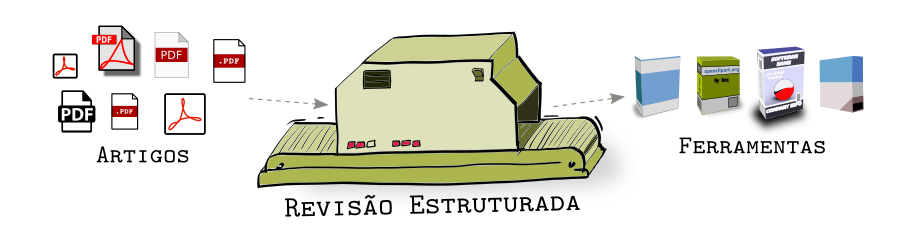
\includegraphics[scale=0.21]{imagens/revisao-estruturada.png}
  \caption{Atividades da revisão estruturada}
  \label{figura-revisao-estruturada}
\end{figure}

As 3 atividades da revisão estruturada, representadas na Figura
\ref{figura-revisao-estruturada}, apresentam como resultado final um conjunto
de softwares com as seguintes informações:

\begin{itemize}
  \item Nome e descrição do software acadêmico.
  \item Título do artigo onde o software é citado como contribuição, seja principal ou secundária.
  \item Nome e ano da conferência onde o artigo foi publicado.
  \item Endereço onde o software pode ser obtido, páginas web ou repositórios de código fonte.
\end{itemize}

Cada atividade da revisão gera como saída um conjunto de artigos, este conjunto
é reduzido a cada atividade, a última delas gera também um conjunto de
softwares acadêmicos com algumas de suas informações.

Seguem detalhes de cada atividade:

\begin{description}

  \item[(1) Busca]
    A primeira atividade da revisão estruturada define as fontes de entrada,
    estas fontes são conferências que abordam o tema de interesse do estudo, e
    que apresentam um grande potencial de encontrar softwares do domínio de
    aplicação desejado, neste estudo o interesse está em softwares de análise
    estática de código fonte, portanto as conferências selecionadas serão
    aquelas com potencial de se encontrar softwares deste domínio de aplicação.
    Esta primeira atividade deve incluir o maior número possível de ediçoes de
    cada conferência, para cada edição é copiado localmente todos os artigos em
    formato PDF, eles serão utilizados como entrada na atividade 2.

  \item[(2) Filtro]
    A segunda atividade da revisão estruturada realizada em cima de todo o
    conjunto de artigos selecionados na etapa anterior é uma busca pelos
    seguintes termos em todo o conteúdo dos artigos:

    \begin{verbatim}
      "tool" OU "framework"; E
      "download" OU "available"; E
      "http" OU "ftp"; E
      "static analysis" OU "parser".
    \end{verbatim}

    Esses termos devem ser pensados em relaçao ao domínio de aplicação
    desejado, devem ser abrangentes a fim de evitar falsos negativos, ou seja,
    evitar que o filtro deixe de fora artigos que publiquem software de análise
    estática, mesmo que isto resulte em falsos positivos, a atividade seguinte
    identificará esses falsos negativos deixando-os fora do resultado final.

    Esses termos devem encontrar artigos com publicação de softwares
    científicos do domínio de análise estática de código fonte com
    disponibilidade para {\it download}, seja binário ou código fonte, será
    aplicado automaticamente com auxílio de um script desenvolvido durante este
    trabalho de pesquisa, detalhes deste script, outros artefatos produzidos
    durante esta pesquisa, e onde obtê-los pode ser encontrado no Apêndice
    \ref{reproducibilidade-do-estudo}.

  \item[(3) Seleção]
    A terceira e última atividade da revisão estruturada identifica se cada
    artigo resulta, de fato, em publicação de software acadêmico de análise
    estática. Esta seleção é feita a partir de uma leitura superficial do
    artigo em busca de indícios de que o artigo publica de fato algum software.

    Essa leitura inclui título, introdução, resultados e conclusões, o objetivo
    é identificar se o artigo publica software acadêmico e indica onde obter
    uma cópia do software. Quando esta leitura inicial não é o suficiente para
    identificar se há publicação de software, outras seções são lidas, alguns
    artigos descrevem a implementação do software em seções específicas, outros
    indicam detalhes do software ao longo do texto, é comum o uso de
    notas de rodapé para indicar onde o software está disponível. Softwares
    acadêmicos que sejam mais abrangentes do que apenas análise estática de
    código fonte mas que contenham esta função em seu conjunto também são
    selecionados.

\end{description}

Ao final da revisão poderemos responder à questão de pesquisa {\bf Q1}
(\QuestaoUm).

\subsection{Quantificação da disponibilidade dos softwares acadêmicos}

Os softwares acadêmicos selecionados na revisão estruturada foram avaliados em
relação à sua disponibilidade, apenas os softwares com indicação de fonte para
obtenção foram incluídos, dois aspectos foram analisados, um relacionado à como
o artigo cita o software e outro relacionado a como o software está disponível,
código fonte, binários e licença utilizada.

O primeiro aspecto tem o objetivo de identificar se o software está disponível
de fato, se a fonte informada no artigo relacionado ao software está acessível
publicamente e se é possível obter uma cópia do software, cada software
acadêmico será caracterizado entre uma das seguintes opções:

\begin{itemize}
  \item Fonte para obtenção do software indisponível -
    {\it O artigo indica fonte mas encontra-se inacessível, fora do ar ou com erros}
  \item Software disponivel, binários ou código fonte -
    {\it A fonte indicada está disponível e acessível publicamente}
\end{itemize}

O endereço indicado no artigo será acessado a fim de identificar se está
funcional e se é possível obter uma cópia do software, essa avaliação nos dirá
o quanto permanecem disponíveis os softwares publicados na literatura
acadêmica, lembrando que pequenos scripts ou protótipos sem indicação de
endereço para obtenção não foram considerados neste estudo, a revisão
estruturada, responsável pelo conjunto de softwares selecionados, preocupa-se
apenas em encontrar softwares acadêmicos citados pelo próprio autor como uma
das contribuições do seu estudo, e que tenha sido citado com endereço para
obtenção do mesmo.

Isto nos permitirá responder à questão de pesquisa {\bf Q2} (\QuestaoDois)
e {\bf Q3} (\QuestaoTres).

%Mesmo que o autor tenha disponibilizado fontes para obtenção dos artefatos produzidos,
%o fato de não informarem a fonte inviabiliza, ou ao menos dificulta, bastante
%pesquisadores interessados em repetir ou reproduzir os resultados de tais estudos.

O segundo aspecto diz respeito à como o
software está disponível, é um nível de detalhe sobre o primeiro aspecto, os
softwares caracterizados como disponíveis no primeiro aspecto serão detalhados
aqui, informando de que forma estão disponíveis, se código fonte, ou apenas
binários.

\begin{itemize}
  \item Código fonte disponível
  \item Apenas binários disponível
\end{itemize}

%Esse segundo aspecto toma como base o trabalho de \citeonline{Novak2010} em que
%propõe uma taxonomia e um conjunto de dimensões para caracterização de
%ferramentas de análise estática, uma das dimensões para caracterização
%é esta relacionado à como o software é disponibilizado.

Lembrando que apenas os softwares caracterizados no primeiro aspecto como
{\it``software disponivel, binários ou código fonte''} serão detalhados aqui.
Os softwares caracterizados como {\it ``código fonte disponível''} incluirão
qualquer softwares mesmo sem licença definida, não estamos avaliando neste
momento se o software é livre ou aberto segundo as definições de software {\it
livre} e {\it open} da Free Software
Foundation\footnote{\url{https://www.gnu.org/philosophy/free-sw.html}} e Open
Source Initiative\footnote{\url{https://opensource.org/osd}}, respectivamente,
o acesso ao código fonte é a característica de interesse neste estudo, com ele
é possível estudar o conhecimento empregado nos softwares, bem como repetir o
estudo original utilizando ou executando tal código quando necessário.

Nos dando indícios para responder a questão de pesquisa {\bf Q4}
(\QuestaoQuatro).

A fonte para coleta dessas informações serão os artigos relacionados aos
softwares, código fonte, documentos e site do projeto, quando disponíveis.

\section{Resultados}

Na revisão estruturada selecionamos a conferência SCAM - {\it
Source Code Analysis and Manipulation Working
Conference}\footnote{\url{http://www.ieee-scam.org}} e a conferência ASE - {\it
Automated Software Engineering}\footnote{\url{http://ase-conferences.org}},
ambas conferências com largo histórico de publicação sobre análise de
programas e apresentam um alto potencial de encontrar softwares do domínio de
análise estática de código fonte.

A primeira atividade da revisão estruturada -- (1) Busca -- passa por
todas as ediçoes das duas conferências até o ano de 2015, ou seja, explora o
histórico de 24 anos de publicação. Todas as trilhas de ambas as conferências
foram incluídas, encontramos nesta atividade 1873 artigos no total, 1527 artigos
do ASE e 346 artigos do SCAM, com uma média geral de 75 artigos publicados por ano. A
Figura \ref{artigos-por-ano} apresenta a distribuição por edição de cada
evento.

\begin{figure}[h]
  \center
  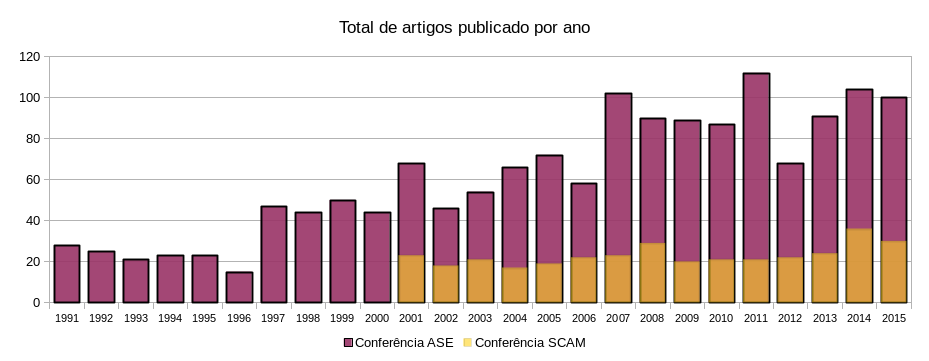
\includegraphics[scale=0.65]{imagens/artigos-por-ano.png}
  \caption{Gráfico em barras com o total de artigos publicado por ano}
  \label{artigos-por-ano}
\end{figure}

Entre os anos de 1991 e 1996 a conferencia ASE chamava-se KBSE - {\it
Knowledge-Based Software Engineering Conference} e só a partir de 1997 passou a
chamar-se ASE - {\it Automated Software Conference}. A edição com o maior
número de publicações foi 2011 com 112 artigos publicados, seguido de 2014 com
104, e 2007 com 102, a edição com o menor número foi 1996 com apenas 15 artigos
publicados.

A conferência SCAM teve sua primeira edição apenas em 2001, 10 anos após a
primeira edição do ASE, e possui uma média de 23 artigos publicados por edição.
Se compararmos os mesmos períodos de ambas as conferências, 2001 à 2015,
percebemos que a conferência ASE publica quase 4 vezes mais do que a
conferência SCAM. Neste período a conferência ASE teve uma média de 80 artigos
publicados por ano, se for levado em conta todas as edições, apenas da
conferência ASE, a média cai para 61 artigos por ano.

A segunda atividade da revisão estruturada -- (2) Filtro -- reduziu em 77\%
o número total de artigos de forma automática a partir da string de busca, resultando em 441 artigos
para serem analisados na próxima etapa da revisão estruturada.  Durante a execução desta
atividade foi necessário analisar dois artigos manualmente, {\it Adaptable
concern-based framework specialization in UML} e {\it Property-oriented test
generation from UML Statecharts}. O conteúdo destes dois artigos não é possível
de ser analisados pelo script de filtro uma vez que é formado por imagens
digitalizadas, ambos artigos publicados no ASE edição 2004. Nenhum dos dois
artigos continham os termos pesquisados e ficaram fora do conjunto selecionado
nesta atividade.

A terceira e última atividade da revisão estruturada -- (3) Seleção --
realizada em cima dos 441 artigos selecionou 107 artigos com publicação de
software científico do domínio de aplicação de análise estática, alguns destes
artigos fazem referência à um mesmo software, é o caso do {\it BEST: A symbolic
testing tool for predicting multi-threaded program failures} e do {\it Scalable
and precise symbolic analysis for atomicity violations}, ambos publicados no
ASE 2011 fazem referência ao software BEST. Situação similar ocorreu com o {\it Augmenting
Counterexample-Guided Abstraction Refinement with Proof Templates} e o {\it
PtYasm: Software Model Checking with Proof Templates} publicados no ASE 2008,
fazem referência ao software PtYasm. Por conta disso, entre os 107 artigos, temos
105 softwares distintos, uma lista com todos os softwares e uma breve descrição
de cada um é apresentado no Apêndice \ref{resumo-softwares},
detalhes sobre o número de artigos e softwares encontrados em cada conferência
pode ser consultados nos Apêndices \ref{artigos-do-scam} e \ref{artigos-do-ase} 

Ainda durante esta atividade da revisão cada um dos 107 artigos foram
analisados em busca de informações sobre onde encontrar o software indicado,
esta análise resultou em 60 softwares com indicação de fonte para obtenção do
software, todos os artigos indicam endereço de página web para download do
software. A Figura \ref{softwares-por-ano} apresenta estes 60
softwares distribuídos ao longo dos anos num gráfico em linha.

\begin{figure}[h]
  \center
  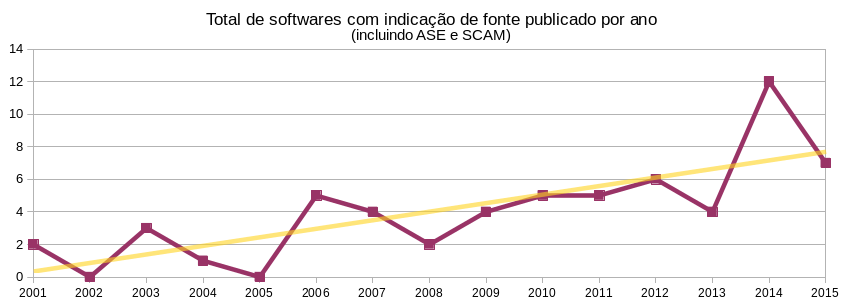
\includegraphics[scale=0.65]{imagens/softwares-por-ano.png}
  \caption{Gráfico em linha com o número de softwares por ano selecionados na revisão estruturada}
  \label{softwares-por-ano}
\end{figure}

É possível perceber um certo crescimento no número de softwares publicados com
o passar dos anos, ao menos em softwares do domínio de análise estática, de
forma que podemos confirmar que considerando as conferências ASE e SCAM, há um
crescimento na publicação de softwares acadêmicos ao longo do tempo, nos dando
oportunidade de responder parte da questão de pesquisa {\bf Q1} (\QuestaoUm).

Apesar da busca na atividade -- (2) Filtro -- utilizar termos com o objetivo de
encontrar apenas softwares disponíveis com informação de onde encontrar o
software, ainda assim, encontramos 45 artigos com publicação de software sem
indicação de fonte para obtenção.

Entre os 1873 artigos, encontramos 107 artigos referenciando 105 softwares de
análise estática, apenas 60 destes indicam fonte onde o software pode ser
encontrado, apenas 37 estão disponíveis, os 23 restantes indicam fonte não mais
acessíveis, endereço não encontrado, indisponível, ou com informações não
relacionadas ao software. O Apêndice \ref{resumo-softwares-disponiveis} traz
uma tabela com os nomes e endereços web onde os softwares estão disponíveis.

Esta informação nos permite responder a questão de pesquisa {\bf Q2}
(\QuestaoDois), levando em conta a sustentabilidade técnica podemos responder que 61\% dos
softwares produzidos no domínio de aplicação de análise estática são
sustentáveis, ou seja, continuam disponíveis ao longo do tempo. Lembrando que
não está sendo considerado aqui pesquisas que publicam software sem menção à
fonte onde pode ser encontrado, a revisão estruturada teve como foco encontrar
artigos com publicação softwares com indicação de fonte, ou seja, aqueles
artigos que publicam software mas que não indicam fonte não está sendo
considerado aqui, vimos que na revisão estruturada, mesmo não sendo o objetivo
encontramos 45 artigos sem informação de fonte, isto faria esta taxa cair para
apenas 35\%, uma revisão estruturada mais abrangente com objetivo de encontrar
todo e qualquer software, independente de indicar fonte ou não, com certeza
faria esta taxa cair abaixo dos 35\%.

\citeonline{robles2010replicating} afirma que existe uma tendência das páginas
web onde os softwares estão disponíveis tem uma grande chance de se tornarem
indisponíveis ao passar do tempo, podemos investigar esta tendência 
avaliando os 60 softwares com fonte indicada no artigo,
identificar se confirmamos neste contexto se com a idade do paper
as páginas web onde os softwares são publicados tem uma grande chance de se
tornarem indisponíveis ao passar do tempo.

\begin{figure}[h]
  \center
  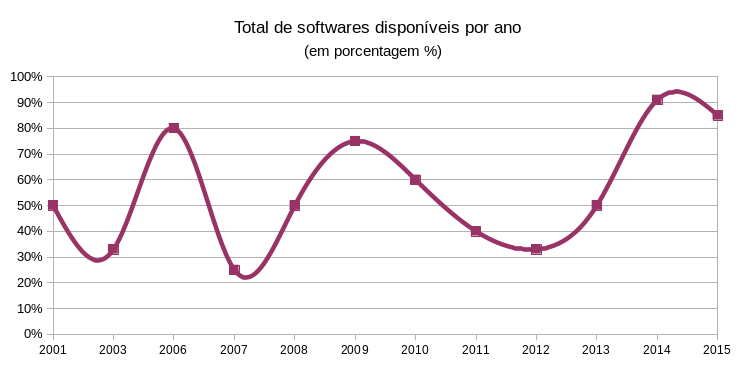
\includegraphics[scale=0.65]{imagens/softwares-disponivel-por-ano.png}
  \caption{Gráfico em linha com o total de softwares disponíveis por ano}
  \label{softwares-disponivel-por-ano}
\end{figure}

A Figura \ref{softwares-disponivel-por-ano} apresenta em cada ano quantos
porcentos do total de softwares publicados com indicação de fonte estão ainda continuam
disponíveis hoje, ou seja, quantos qual é a taxa de softwares que continuam
disponíveis hoje dentro do conjunto de softwares publicados em cada ano com
informação sobre fonte para download.  Os anos de 2002, 2004, 2005, e
anteriores a 2001 não possuem softwares publicados com fonte indicada no artigo
ainda disponível, portanto não constam no gráfico suas informações.

Ao analisar a figura percebemos que há um leve crescimento na disponibilidade
dos softwares nos anos mais recentes, com isso podemos responder à nossa
questão de pesquisa {\bf Q3} (\QuestaoTres).

Existe uma leve tendência da fontes informadas, páginas web, se tornarem
indisponível ao longo do tempo, é possível notar que em 2006 80\% de todos os
softwares de análise estática publicados estão ainda disponíveis, este número
cresce em 2014 chegando a 90\%, e cai no ano seguinte para 85\%, apesar de não
estar sempre crescente, e de termos uma amostra pequena, apenas 60 softwares,
este leve indício confirma a afirmação de \citeonline{robles2010replicating}.

Esses 37 softwares com fonte disponível foram avaliados em relação ao segundo
aspecto em respeito à de que forma estão disponíveis, os artigos informam onde
obter tais softwares, os softwares estão realmente disponíveis, as fontes
indicadas foram acessadas e na presente data deste trabalho estão funcionando e
acessíveis, mas queremos saber em qual formato estes softwares estão
disponíveis?

\begin{itemize}
  \item Código fonte disponível
  \item Apenas binários disponível
\end{itemize}

Entre estes apenas 3 não possuem código fonte disponível, 34 estão com o código
fonte disponível publicamente, dentre elas 13 não informam licença alguma
apensar de ter o código fonte disponível, 21 informam licenças de FOSS ({\it
free and open source software}):

\begin{itemize}
  \item 8 usam GNU General Public License;
  \item 2 usam Apache License;
  \item 4 usam BSD License;
  \item 3 usam Eclipse Public License;
  \item 2 usam University of Illinois/NCSA Open Source License;
  \item 1 usa licença {\it FrontEndART Software Ltd}; e
  \item 1 usa licença {\it SAnToS Laboratory Open Academic License}.
\end{itemize}

Com essas informações podemos responder à terceira e última questão de
pesquisa desse estudo {\bf Q4} (\QuestaoQuatro).

Entre os 37 softwares disponíveis 21 podem ser modificados para se adaptar às
necessidades emergentes sem necessidades de solicitação prévia de autorização
aos autores originais devido ao uso de licenças livres. Os 13 softwares
restantes com código fonte disponível mas sem licença expressa podem
eventualmente serem modificados mas a falta de uma licença impõe à necessidade
de solicitar permissão aos autores originais.

35\% dos softwares disponíveis podem ser adaptados de forma incremental para
aproveitar oportunidades emergentes, 21\% podem mediante prévia autorização do
autor original serem modificados, e apenas 5\% não oferecem essa possibilidade
por não disponibilizarem o código fonte publicamente.

\section{Ameaças à validade}

Estamos considerando que o código fonte é necessário para repetir um dado
estudo mas pode ser que em alguns casos o estudo possa ser repetido mesmo sem a
disponibilidade do mesmo, isto poderia ser resolvido realizando a repetição
de cada estudo na prática e a partir daí identificar se o código fonte dos
softwares desenvolvidos são requeridos.

A escolha de um domínio de aplicação específico para seleção dos softwares
pode ser um fator de influencia nos resultados obtidos, sendo possível que
o número de artigos com publicação de softwares com código fonte disponível
encontrado não reflita nos outros domínios, os problemas diagnosticados
neste domínio pode não ser verdade em outros domínios, sendo necessário
realizar o mesmo estudo em outros domínios.

A leitura dos artigos na revisão estruturada para identificar se publicam
softwares de análise estática de código fonte, se disponibilizam fonte para
obtenção de tais softwares, e se os softwares são mesmo do domínio de aplicação
de análise estática de código fonte podem ter maior validade se feitos em
par e revisados por outros pesquisadores, neste estudo tudo foi feito pelo
autor deste estudo e não houve revisão por pesquisadores independentes.

\section{Conclusões}

Dos 346 artigos do SCAM e 1533 artigos do ASE analisados na revisão estruturada
apenas 44\% (155 artigos) e 18\% (281 artigos) continham os termos pesquisados
no filtro automático da segunda atividade da revisão, respectivamente.

Deste total apenas 11\% (41 artigos) e 4\% (62 artigos) foram selecionados na
terceira e última atividade da revisão contendo publicação de ferramenta de
análise estática.

Resultando em 103 artigos com publicação de {\it software científico} de
análise estática de código fonte, apenas 35 possuem fonte para obtenção do
software, sendo 32 de código aberto, ou seja, com disponibilidade de
código fonte, e 3 grátis, apenas binários disponível. Ou seja, apenas 31\% dos
artigos com publicação de software disponibilizam o código fonte das mesmas.
Isto significa que 69\% dos artigos com publicação de software de análise
estática de código fonte são potencialmente impossíveis de serem repetidos, já
que os artefatos originais são necessários para tal atividade e o artigo não
disponibiliza o código fonte dos mesmos.

% o artigo com resumo do RESER 2011 diz \cite{knutson2010report}:
% 4) Re-
% search tools are either not available or not usable, so precise
% replication is impractical [1, 2, 8, 18, 19].

Muitos outros aspectos podem ser levados em consideração quando se está
avaliando a capacidade de repetir ou replicar um estudo, aqui avaliamos apenas
a disponibilidade de código fonte dos softwares científicos, mas inúmeros detalhes
pormenores são necessários, tais como: indicar qual versão do software foi
utilizado no estudo, 

No entando, consideramos que nem todos os scripts e código fonte pode
valer o custo de dua publicação, sabe-se que umas das barreiras para publicação
de muitos destes artefatos são as dificldades em tal atividade,
e as objeções a tal prática de ter RR reques um esforço adicional \cite{madeyski2017would},
em muitos
estudos o simples fato de não possuir código disponível pode não levar
a problemas para alcançar a meta final que é aumento da validade do estudo,


Todas as atividades e artefatos produzidos neste estudo estão documentados em
repositório público no
Github\footnote{\url{http://github.com/joenio/dissertacao-ufba-2016}}, o
Apêndice \ref{apendice-revisao-estruturada} traz mais informações.

%, uma lista completa e
%o endereço de cada edição onde os artigos foram obtidos está documentado no
%Apêndice \ref{edicoes-conferencias}

% IDEIA!
% levantar ano de publicação do artigo para cada software e
% calcular por quanto tempo cada software está disponível,
% com isso verificar se há um padrão, ou seja, se publicações
% mais antigas possuem softwares não-disponíveis, obsoletos,
% etc...
              % execution

%------------------------------------------%

\xchapter{Análise da complexidade estrutural dos softwares científicos}
{Este capítulo apresenta uma análise da complexidade estrutural dos softwares
científicos de análise estática de código-fonte como forma de avaliar a qualidade
interna dos mesmos.}
\label{complexidade-ferramentas}

Poucos estudos sobre avaliação de qualidade interna de softwares fazem isso com
{\it softwares científicos}, algo de extrema importância para compreender como
tais artefatos estão contribuindo para a divulgação do conhecimento e para
replicação dos resultados das pesquisas em engenharia de software.

Avaliar os {\it softwares científicos} do ponto de vista de sua qualidade pode
ajudar a compreender quanta atenção é dada ao seu desenvolvimento, uma vez que
tradicionalmente os seus autores enfrentam problemas com manutenabilidade
\cite{Prlic2012}.

Manutenabilidade é uma característica de qualidade externa que indica o quão
fácil é realizar atividades de evolução e manutenção em componentes de
software, ela pode ser medida através de características de qualidade interna,
uma vez que grande parte dos engenheiros de software assumem que uma boa
estrutura interna resulta em boa qualidade externa \cite{Fenton2014}. A
estrutura interna de um software pode ser avaliada através da sua complexidade,
uma característica bastante referenciada na literatura como um importante
indicador de qualidade, estudos mostram que quanto maior a complexidade, maior
é o esforço de manutenção \cite{hashim1996software, Darcy2005}, em especial a
complexidade estrutural, uma medida definida em termos de acoplamento e coesão
\cite{Terceiro2012}.

Assim temos como objetivo neste estudo avaliar a qualidade dos {\it softwares
científicos} a partir de sua complexidade estrutural.

Os softwares avaliados neste estudo serão do domínio de aplicação de análise de
código-fonte, ferramentas de análise estática de código-fonte tem sido
continuamente desenvolvidas e tem se tornado mais e mais comuns no ciclo de
desenvolvimento de software \cite{Novak2010}, e apesar da rápida e constante
evolução da área, ainda há carência de estudos avaliando estas ferramentas
\cite{Li2010}, especialmente os {\it softwares científicos}.

% referencia sobre complexidade:
% Livro: Software Metrics, A Rigorous and Practical Approach [3rd 2015]
% 9.1.1 Structural Complexity Properties
%
%
%We will also
%investigate the maintainability measures taxonomy by
%Oman et al where 92 measures are listed and classified [24].
%[24] Oman, P., Hagemeister, J., and Ash, D., A Definition
%and Taxonomy for Software Maintainability, report
%SETL Report 91-08-TR, University of Idaho, 1991.
%
%\cite{Measurements of Software Maintainability}
%
%Taxonomia, metricas, etc ... sobre manutenabilidade de software.
%
%\cite{Metrics for Assessing a Software System’s Maintainability}

\section{Planejamento do estudo}

Os dados serão coletados através de uma revisão estruturada, análise estática
com o Analizo, e caracterizacao manual das ferramentas a partir das fontes:
artigo, documentação, sites e repositórios da ferramenta.

Além da revisão estruturada, que será a fonte de ferramentas da academia,
iremos também buscar e selecionar ferramentas da indústria, para isto
buscaremos fontes e catálogos através de pesquisa livre na internet.

Coletamos para cada ferramenta selecionada suas métricas de código-fonte
através da execução da ferramenta {\it analizo metrics}, esta coleta foi
automatizada pelo script {\it
analyze-all-projects}\footnote{http://github.com/joenio/dissertacao-ufba-2016/blob/master/dataset/analyze-all-projects}
escrito durante este estudo disponível no
repositório\footnote{http://github.com/joenio/dissertacao-ufba-2016} desta
pesquisa.

\subsection{Analizo} \label{analizo}

Analizo é um conjunto de ferramentas para análise de código-fonte e
visualização com suporte a múltiplas linguagens de programação, software livre,
extensível e capaz de lidar com código-fonte não mais compilável. A capacidade
de lidar com código-fonte não mais compilável permite analisar código-fonte
com erros de sintaxe, com referências a bibliotecas não mais disponíveis, ou
que usem bibliotecas com mudanças de API.

%Ela será a ferramenta utilizada por nós durante este estudo para análise do
%código-fonte das ferramentas selecionadas, a decisão pela ferramenta Analizo
%se deu por conta dela ser também a escolha utilizada nos trabalhos
%relacionados (seção \ref{trabalhos-relacionados}) onde estamos nos apoiando,
%além disso, Analizo também tem sido utilizada em diversos estudos
%desenvolvidos em nosso grupo de pesquisa (seção \ref{trabalhos-analizo}).

\subsubsection{Arquitetura do Analizo}

A arquitetura do Analizo é apresentada na Figura \ref{arquitetura-analizo}
através de uma representação {\it Layered Style} \cite{Clements2002}, cada
camada no diagrama usa apenas os serviços oferecidos pela camada diretamente
abaixo dela.

\begin{figure}[h]
\center
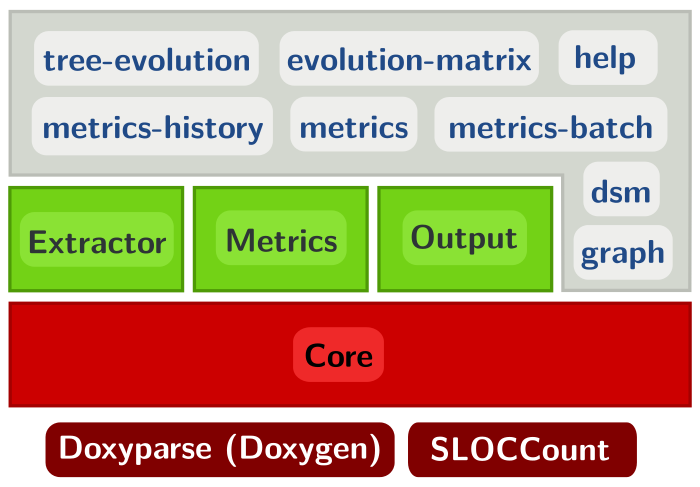
\includegraphics[scale=0.3]{imagens/analizo-architecture.png}
\caption{Arquitetura do Analizo, usando Layered Style \cite{Clements2002}}
\label{arquitetura-analizo}
\end{figure}

O {\it Core} contém as estruturas de dados usadas para armazenar informações a
respeito do código-fonte sendo analisado, lista de módulos\footnote{o
conceito ``módulo'' é usado como um termo abrangente para designar diferentes
tipos de estruturas usados em desenvolvimento de software, como classes e
arquivos fonte C}, elementos dentro de cada módulo (atributos, variáveis,
métodos, funções) e informações de dependência (chamada, herança, etc). Esta
camada implementa a maior parte da lógica de negócio do Analizo, e não depende
de nenhuma outra camada.

A camada {\it Extractor} lida com as informaçoes de código-fonte obtidas pelas
diferentes estratégias implementadas no Analizo. Os extratores obtém
informações do código-fonte e armazenam em estruturas de dados na camada {\it
Core}. Adicionar um novo extrator requer apenas a criação de uma nova subclasse
que faça interface com uma ferramenta externa ou que ela própria realize análise
de código-fonte.

%% Atualmente existem dois extratores, ambos fazem interface
%% com ferramentas externas de análise estática de código-fonte:
%% 
%% \begin{itemize}
%% 
%%   \item {\it Analizo::Extractor::Doxyparse} é uma interface para o Doxyparse,
%%   um parser de código-fonte para C, C++ e Java desenvolvida por nosso grupo de
%%   pesquisa\cite{Costa2009}. Doxyparse é baseado no
%%   Doxygen\footnote{doxygen.org}, um sistema de documentação multi-linguagem.
%% 
%%   \item {\it Analizo::Extractor::Sloccount} é uma interface para o
%%   Sloccount\footnote{dwheeler.com/sloccount} desenvolvido por David A. Wheeler,
%%   uma ferramenta que calcula o número efetivo de linhas de código.
%% 
%% \end{itemize}

A camada {\it Metrics} processa as estruturas de dados do {\it Core} para
calcular métricas, até o momento Analizo suporta um conjunto razoável de
métricas (listadas na Seção \ref{metricas}), uma representação desta camada
pode ser vista no diagrama da Figura \ref{arquitetura-metrics-analizo}.

A camada {\it Output} é responsável por lidar com diferentes formatos de
arquivos.  Atualmente, apenas o formato DOT é implementado no Analizo para
representar grafo de dependencia, adicionar novos formatos é simplesmente
adicionar novas classes nesta camada.

\begin{figure}[H]
\center
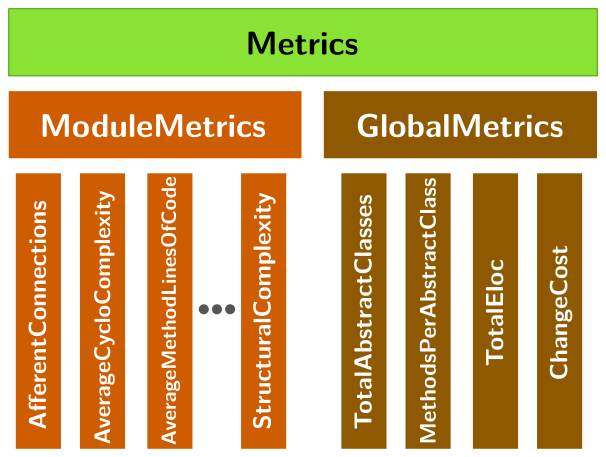
\includegraphics[scale=0.4]{imagens/analizo-metrics-architecture.png}
\caption{Arquitetura do módulo metrics em detalhes, usando Layered Style \cite{Clements2002}}
\label{arquitetura-metrics-analizo}
\end{figure}

A última camada, {\it Tools}, fornece um conjunto de ferramentas de linha de comando que
constituem a interface do analizo, tanto para usuários finais quanto para
aplicações de mais alto nível. Estas ferramentas usam serviços providos pelas
outras camadas: eles instanciam as estruturas de dados do {\it Core},
inicializam um ou mais extratores, opcionalmente executam o processador de
métricas, instanciam um módulo de formato de saída, e gerencia todos eles para
prover o resultado desejado. A maioria das funcionalidades descritas na Seção
\ref{funcionalidades} são implementadas nesta camada.

Estas ferramentas são pensadas na filosofia UNIX: fazem uma tarefa
especializada e geram uma saída que pode ser utilizada como entrada para outras
ferramentas, seja para o próprio Analizo ou para ferramentas externas. Algumas
das ferramentas implementadas no Analizo são feitas consumindo saída gerada por
outra ferramenta, outras são desenhadas para prover saída em formato específico
para aplicações externas, por exemplo, programas para desenho de grafos ou
visualização de dados.

\subsubsection{Funcionalidades}\label{funcionalidades}

\begin{itemize}

\item {\bf Análise de código-fonte multi-linguagem}

Atualmente Analizo suporta análise de código-fonte escrito em C, C++ e Java.
Entretanto, pode ser facilmente estendido para suportar outras linguagens pois
pode potencialmente suportar as inúmeras outras linguagens suportadas pelo Doxygen.

\item {\bf Métricas}\label{metricas}

O Analizo suporta tanto métricas em nível de projeto, que é calculada para todo o projeto,
quanto métricas em nível de módulos, que é calculado individualmente para cada módulo.
No nível de projeto, Analizo também provê estatística descritiva básica para cada métrica em
nível de módulo: soma, média, mediana, moda, desvio padrão, variância, skewness e kurtosis da
distribuição, valores mínimo e maximo. As seguintes métricas são suportadas até o momento:

\begin{itemize}

  \item Métricas em nível de projeto: Change Cost, Total Abstract Classes,
  Total Coupling Factor, Total Effective Lines of Code, Total Lines of Code,
  Methods per Abstract Class, Total Number of Modules, Total number of modules
  with at least one defined attributes, Total number of modules with at least
  one defined method, Total Number of Methods.

  \item Métricas em nível de módulo: Afferent Connections per Class, Average
  Cyclomatic Complexity per Method, Average Method Lines of Code, Argument with
  'nonnull' attribute passed null, Average Number of Parameters per Method,
  Allocator sizeof operand mismatch, Assigned value is garbage or undefined,
  Bad deallocator, Bad free, Coupling Between Objects, Dead assignment,
  Divisions by zero, Double free, Depth of Inheritance Tree, Dereference of
  null pointer, Dereference of undefined pointer value, Potential buffer
  overflow in call to 'gets', Lack of Cohesion of Methods, Lines of Code,
  Memory leak, Max Method LOC, Number of Attributes, Number of Children, Number
  of Methods, Number of Public Attributes, Number of Public Methods,
  Out-of-bound array access, Offset free, Potential insecure temporary file in
  call 'mktemp', Response for a Class, Result of operation is garbage or
  undefined, Return of stack variable address, Stack address stored into global
  variable, Structural Complexity, Undefined allocation of 0 bytes,
  Use-after-free, Uninitialized argument value.

\end{itemize}

É possível especificar que certos diretórios dentro do projeto não devem ser
analisados, de forma que o Analizo ignore tais arquivos durante a análise e o
cálculo de métricas.

\item {\bf Processamento em lote}\label{lote}

A maioria dos estudos quantitativos em engenharia de software envolve aquisição
de métricas de código-fonte de um grande número de projetos, processar cada
projeto individualmente é pouco prático, passível de erros e difícil de
repetir. Analizo pode processar multiplos projetos em lote e produzir arquivo
de dados CSV com métricas de cada projeto, bem como um resumo com as métricas
em nível de projeto de todos os projetos. Estes arquivos de dados podem ser
facilmente importados em ferramentas de estatística ou planilhas para análise
futura. Esta capacidade de processar em lote pode também ser utilizada para
analisar várias versões de um mesmo projeto, especialmente útil em estudos
sobre evolução de software.

%% Este processamento em lote pode se beneficiar de processamento paralelo dando
%% mais agilidade e na análise e reduzindo o tempo total de processamento.  A
%% saída pode ser também escrita diretamente em um banco de dados relacional ao
%% invés de gerar arquivos CSV. Outro recurso voltado à performance é um sistema
%% de cache para as informações previamente calculadas, evitando repetição de
%% processamento.

\item {\bf Histórico de métricas}

Algumas vezes pesquisadores precisam processar o histórico de projetos de
software de uma forma mais escalável. Analizo pode processar repositórios de
controle de versão e prover arquivo de dados CSV com valores de métricas para
cada revisão onde o código-fonte foi alterado no projeto, ou pode também gravar
os valores diretamente num banco de dados ao invés de usar arquivos CSV. Repositórios Git e
Subversion são suportados diretamente, repositórios CVS devem ser convertidos
para Git de forma manual.

\item {\bf Grafo de dependência}

Analizo pode gerar saída com informações sobre dependência entre as entidades
do projeto em um formato adequado para processamento por ferramentas de
renderização de grafos do Graphviz\footnote{graphviz.org}. A Figura
\ref{sample-graph} apresenta um exemplo de grafo desenhado pela ferramenta {\it
dot} do Graphviz a partir da saída gerada pelo Analizo {\it graph}.

\begin{figure}[h]
\center
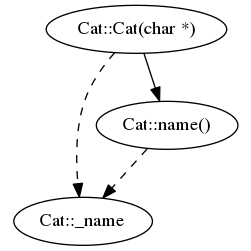
\includegraphics[scale=0.4]{imagens/sample-graph.png}
\caption{Exemplo de grafo de dependência}
\label{sample-graph}
\end{figure}

%% \item {\bf Matriz de evolução}
%% 
%% Outra funcionalidade útil do Analizo é a visualização de matrizes de evolução
%% \cite{Lanza2001}. Ao processar cada release de um projeto (ver Seção
%% \ref{lote}), o usuário pode solicitar a criação de uma matriz de evolução a
%% partir de arquivos de dados individuais. A Figura \ref{sample-evolution-matrix}
%% apresenta um exemplo de uma matriz produzida pelo Analizo.
%% 
%% \begin{figure}[h]
%% \center
%% 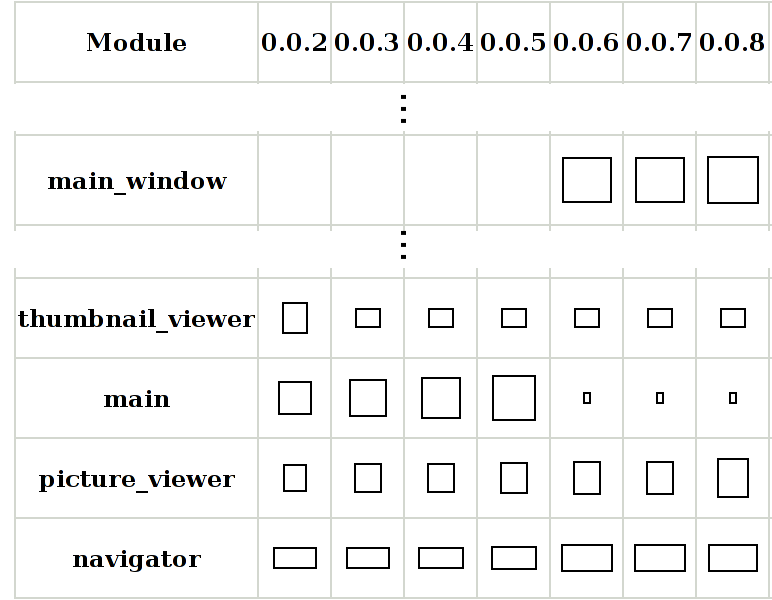
\includegraphics[scale=0.2]{imagens/sample-evolution-matrix.png}
%% \caption{Exemplo de matriz de evolução}
%% \label{sample-evolution-matrix}
%% \end{figure}
%% 
%% \item {\bf Matriz de estrutura de projeto}
%% 
%% Uma funcionalidade recente do Analizo é a representação visual do
%% relacionamento entre os módulos do projeto em forma de uma matriz de estrutura
%% de projeto ({\it Design Structure Matrix}) \cite{Maccormack2006}, uma DSM é a
%% representação de um grafo de dependência em forma de uma matriz quadrada. Um
%% exemplo gerado pelo Analizo pode ser visto na Figura \ref{sample-dsm}.
%% 
%% \begin{figure}[h]
%% \center
%% 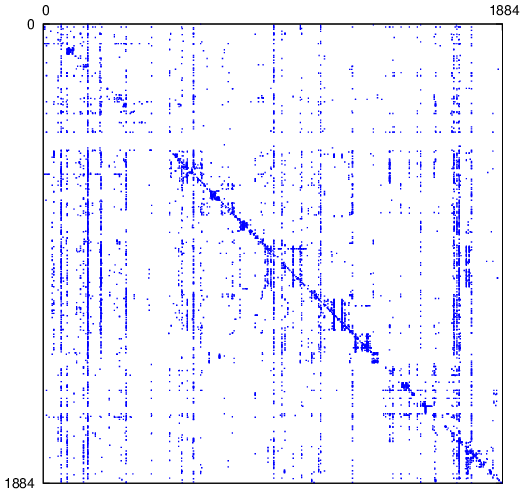
\includegraphics[scale=0.3]{imagens/sample-dsm.png}
%% \caption{Exemplo de matriz de estrutura de projeto}
%% \label{sample-dsm}
%% \end{figure}

\end{itemize}

\subsubsection{Uso em trabalhos de pesquisa}
\label{trabalhos-analizo}

Analizo tem sido extensivamente usado por nosso grupo de pesquisa em diversos
estudos:

\begin{itemize}

  \item \cite{Amaral2009} usou o grafo de dependencia gerado pelo Analizo para
  gerar uma matriz de evolução em um estudo de caso com o projeto VLC.

  \item \cite{Costa2009} fez uma comparação entre diferentes estratégias para
  extração de informação de dependencias entre módulos do código-fonte,
  resultando no desenvolvimento do Doxyparse - o extrator baseado no Doxygen do
  Analizo.

  \item \cite{Terceiro2009} usou métricas em um estudo exploratório sobre a
  evolução da complexidade estrutural em projetos de software livre escritos em
  C.

  \item \cite{Morais2009} usou a ferramenta de métricas do Analizo como backend
  para o Kalibro, um software para avaliação e observação de métricas de código-fonte.
  
  \item \cite{Terceiro2010} usou o processamento de histórico de métricas para
  realizar um estudo exploratório sobre a evolução da complexidade estrutural em
  7 projetos de servidor web de diferentes tamanhos.

  \item \cite{Meirelles2010} usou o processamento em lote do Analizo para
  processas o código-fonte de mais de 6000 projetos de software livre do
  repositório Sourceforge.net.

  \item \cite{Meirelles2011} usou o Analizo em um estudo sobre impacto de
  métricas de código-fonte na atratividade de projetos de softwares livres.

  \item \cite{Terceiro2012Understanding} usou o Analizo para investigar fatores
  que influenciam na evolução da complexidade estrutural em projetos de software
  livres.

  \item \cite{Silva2012} usou o Analizo para minerar 16000 revisões de
  repositórios de projetos de software para investigar o potencial de uma nova
  métrica chamada Lack of Concern-based Cohesion.

  \item \cite{Ronaldo2015} utilizou o Analizo para extrair métricas de
  código-fonte de 14 versões do sistema Android e estudar a evoluçao da API e
  seus aplicativos.

\end{itemize}

A maioria destes trabalhos contribuíram com melhorias para o Analizo, fazendo
dele uma ferramenta bastante apropriada para pesquisas envolvendo análise de código-fonte,
sendo útil tanto para pesquisadores trabalhando com análise de código-fonte
quanto para profissionais que precisam analisar seus projetos em busca de
potenciais problemas ou melhorias.

Analizo é software livre, distribuído sob a licença GNU General Public License
versão 3. Seu código-fonte, bem como pacotes binários, manuais e tutoriais
podem ser obtidos em \url{http://www.analizo.org}. Todas as ferramentas são
auto-documentadas e podem ser consultadas como páginas de manual UNIX. Analizo
é escrito em Perl, sua última versão 1.19.1 lançada em 01 de Setembro de 2016
será a versão utilizada neste estudo.

\section{Análise dos dados} \label{analise}

Os dados coletados incluem a caracterização das ferramentas de análise
estática, bem como, os valores das métricas de código-fonte de complexidade
estrutural para cada ferramenta. A coleta das métricas de
código-fonte será realizada pelo Analizo com o auxílio do script {\em
analyze-all-projects}\footnote{http://github.com/joenio/dissertacao-ufba-2016/blob/master/dataset/analyze-all-projects},
escrito durante o desenvolvimento deste estudo. A caracterização será feita a
partir dos artigos selecionados na revisão estruturada, documentação, site do
projeto e repositório das ferramentas.

Todos os dados serão agregados numa planilha, a análise exploratória será
realizada comparando pares de ferramentas de tamanhos similares, o tamanho das
ferramentas será dado pelo número de módulos. O tamanho deve ser
levado em conta pois sabe-se que ele influencia nos valores de métricas de
código-fonte, complexidade estrutural, por exemplo, sofrem
de tal infuência.

Outro fator de grande influência é o domínio de aplicação, como estamos
estudando apenas ferramentas de análise estática, considera-se que este fator
está isolado e não sofreremos sua influência.

Uma vez que tenhamos o conjunto de pares de ferramentas de tamanhos similares
iremos analisar os valores das métricas de complexidade estrutural e custo de
mudança para cada par e interpretar qual das ferramentas possui melhor
manutenabilidade, partimos do princípio que valores menores para cada uma
destas métricas implicam em melhor manutenabilidade.

Esta análise dos pares irá apenas nos dizer quais ferramentas tem melhor
manutenabilidade em comparação com as demais, não é uma informação que
pode ser interpretada de forma geral, ela não diz que a ferramenta tem
ou não uma boa manutenabilidade, indica apenas que uma certa ferramenta
tem melhor manutenabilidade que uma outra.

Com o conhecimento de quais ferramentas tem melhor manutenabilidade iremos
utilizar as dimensões caracterizadas para cada ferramenta para verificar se
tais características influenciam na manutenabilidade, não apenas notar se
influenciam, mas poderemos notar quais características influenciam. Por
exemplo, será que as ferramentas que aceitam como entrada análise da linguagem
Java possuem melhor manutenabilidade do que aquelas que aceitam C++?

Assim, iremos analisar e interpretar cada par de ferramenta de tamanho
similar, sempre à luz de suas características a fim de compreender quais
características influenciam em sua manutenabilidade.

Com isso temos 11 projetos, destes iremos analisar longitudalmente
as releases e a evolucao dos valores de SC e CC (Change Cost), sao elas:

WALA                     13 releases
error-prone              13 releases
JastAdd                  13 releases
SPARTA                   13 releases
Indus                    (poucos releases, deixando fora da analise longitudinal)
Kiasan/Bogor             (mudou a forma de distribuir ao longo dos releases, dificil obter de forma consistente as versoes)
Lotrack                  (sem releases, poucos commits no github, apenas 11)
PtYasm                   (nao tem releases disponivel, apenas a ultima versao)
srcML                    (releases nao encontrado)
GumTree                  (tem apenas 2 releases do repositorio github)
Sonar Qube Plug-in       (apenas 4 releases no github)
CIVL                     13 releases
CodeBoost                (poucos releases, apenas 6 versoes para download no site)
2LS                      (poucos releases, apenas 7)

% aproveitar perte destas referencias ao justificar o uso de percentis ao inves de média
%
%Observar métricas de código-fonte em nível de projetos de software leva
%ao seguinte desafio: como obter valores de métricas que representem todo o projeto sendo
%que métricas de código-fonte usualmente são calculadas para cada elemento do sistema, como arquivos ou classes?
%
%Este desafio tem sido amplamente discutido em estudos sobre definição de
%intervalos de referência ({\it thresholds}) para métricas de
%código-fonte \cite{Shatnawi2010, Kaur2013, Herbold2011}. Intervalos de
%referência são valores conhecidos para uma dada medida
%\cite[Chapter~2.1]{Lanza2007} com algum valor semantico, por exemplo, se
%medirmos a altura das pessoas e definirmos até 2 metros como alto, então
%pessoas acima de 2 metros serão classificadas como muito altas.
%
%Intervalos de referência podem ser definidos de diversas formas, desde
%abordagens baseadas em modelos estatísticos \cite{Shatnawi2010, Kaur2013}
%até aprendizado de máquina \cite{Herbold2011} e inteligência artificial.
%Entre as inúmeras abordagens, muitas partem de estudos empíricos
%usando softwares da indústria como objeto de estudo, geralmente com
%softwares de domínios específicos, parte-se da coleta de dados de
%métricas de código-fonte e com uso de uma abordagem, ou uma combinação entre
%elas, chega-se aos intervalos.
%
%Estes intervalos são também continuamente avaliados a fim de saber se são
%válidos ou não, as abordagens utilizadas para calcular os intervalos levam em
%consideração inúmeros aspectos na tentativa de validar os valores encontrados,
%como por exemplo a natureza dos dados, se seguem a lei de distribuição de
%potência
%\cite{Wheeldon2003,Potanin2005,Concas2007,Ferreira2009,Yao2009,Clauset2009} ou
%seguem uma distribuição normal
%\cite{Baxter2006,Lanza2007,Herraiz2011,Herraiz2012}, avaliam ainda se possuem
%cauda longa, se são livre de escala, entre outros aspectos.

\section{Resultados}

(pendente)

\section{Ameaças à validade}

(pendente)

\section{Conclusões}

(pendente)

%% usar a dimensao abaixo para definir quais usar na avaliacao longitudinal:
%% 
%% %, e qual a frequência de lançamentos indicando se são
%% %atualizadas frequentemente ou estão obsoletas.
%% 
%% \begin{description}
%% 
%%   \item {\it Lançamentos ({\it Releases}) - quantos lançamentos por ano:}
%%     \begin{itemize}
%%       \item Frequentemente $>=$ 3 vezes ao ano\\
%%         {\it \small novas versões da ferramenta são lançadas 3 ou mais vezes por ano}
%%       \item Ocasionalmente $<$ 3 vezes ao ano\\
%%         {\it \small novas versões da ferramenta são lançadas menos que 3 vezes ao ano}
%%       \item Obsoleta 0 vezes ao ano\\
%%         {\it \small intervalo entre novos lançamentos é maior que 1 ano}
%%     \end{itemize}
%% 
%% \end{description}
%% 
%% O autor não deixa claro como categorizar softwares sem lançamentos nos últimos
%% anos mas com histórico de lançamento frequente em anos anteriores. Assim, será
%% considerado todo o histórico de lançamentos e só serão considerados obsoletos
%% por exemplo softwares que nunca tenha tido mais de 1 lançamento ao ano
%% considerando todo o histórico dele. Da mesma forma, será considerado ocasional
%% apenas aqueles que sempre tiveram no máximo 2 lançamentos ao ano. Esta dimensão
%% irá nos dizer o grau de evolução de cada ferramenta, considerando que softwares
%% com lançamentos frequentes estão evoluindo.
%% 
%% ======================
%% 
%% \begin{description}
%% 
%%   \item {\it Entrada - quais tipos de arquivos podem ser carregados na ferramenta:}
%%     \begin{itemize}
%%       \item Código-fonte - arquivos de código texto podem ser carregados
%%       \item Byte code - arquivos com Java Byte Code ou Microsoft
%%       \item Linguagem intermediária (MSIL) pode ser carregada
%%     \end{itemize}
%% 
%%   \item {\it Linguagens suportadas - quais linguagens de programação a ferramenta suporta:}
%%     \begin{itemize}
%%       \item .NET - todas as linguagens compiladas em bibliotecas ou programas no framework .NET
%%       \item VB .NET - suporta VB.NET
%%       \item C\# - suporta C\#
%%       \item Java - suporta linguagem de programação Java
%%       \item C, C++ - suporta linguagem de programação C ou C++
%%     \end{itemize}
%% 
%% \end{description}
%% 
%% As dimensões apresentada por \citeonline{Novak2010} não cobrem alguns aspectos
%% importantes percebidos ao longo deste estudo, assim novas dimensões serão utilizadas
%% em complemento às dimensões citadas acima.
%% 
%% \begin{description}
%% 
%%   \item {\it Linguagem de programação - em que linguagem de programação à ferramenta é escrita:}
%%     \begin{itemize}
%%       \item .NET
%%       \item VB .NET
%%       \item C\#
%%       \item Java
%%       \item C, C++
%%     \end{itemize}
%% 
%% \end{description}
%% 
%% 
%% ================
%% 
%% 
%% A ferramenta livre {\it sloccount}\footnote{http://www.dwheeler.com/sloccount}
%% foi utilizada para identificar a linguagem de programação em que cada
%% ferramenta é implementada. O tamanho em número de classes foi extraído utilizando a ferramenta
%% Analizo, uma das inúmeras métricas que ela extraí é a contagem do número total
%% de classes de um sistema. 
%% 
%% ===============
%% 
%% \section{Data collection procedure}
%% 
%% \begin{itemize}
%%   \item Pesquisa livre em fontes na internet para busca e seleção de ferramentas da indústria
%%   \item Obtenção do código-fonte de cada ferramenta
%%   \item Cálculo e coleta de métricas de código-fonte
%%   \item Obtenção de código-fonte de mais versões de ferramentas com {\it Lançamentos} frequentes ou ocasionais
%%   \item Cálculo e coleta de métricas de código-fonte das novas versões
%% \end{itemize}
%% 
%% ==============
%% 
%% \subsection{Analizo}
%% 
%% Numa primeira análise dos valores coletados pelo Analizo notamos uma anomalia
%% nos valores da métrica CBO, o que nos levou a investigar de perto os motivos,
%% esta anomalia se apresentava como valores extremamente altos para esta métrica,
%% bastante discrepante com as demais métricas calculadas.
%% 
%% Para entender se estes valores estavam corretor ou não, utilizamos uma outra
%% ferramenta para cálculo das métricas, em nossos estudos encontramos e
%% utilizamos uma versão de avaliação da ferramenta {\it SciTools
%% Understand}\footnote{http://scitools.com/trial-download-3} em sua versão
%% ``4.0.853'' em Linux 64 bits. Os dados extraídos por esta ferramenta podem ser
%% encontrados em nosso
%% repositório\footnote{http://github.com/joenio/dissertacao-ufba-2016/tree/master/dataset/Understand
%% SciTools}. Eles demonstraram que os valores calculados pelo Analizo estavam
%% bastante alto em comparação com as demais métricas.
%% 
%% Assim, descobrimos que o Analizo tinha de fato um erro no cálculo da métrica
%% CBO, erro que foi corrigido durante este estudo e disponibilizado na versão
%% mais recente do Analizo, versão que está sendo utilizada aqui.
%% 
%% 
%% =============
%% 
%% \subsection{Ferramentas da indústria}
%% 
%% Em paralelo à revisão estruturada para seleção de ferramentas da academia
%% foi realizada uma seleção manual no catálogo de ferramentas de análise estática do projeto
%% SAMATE\footnote{https://samate.nist.gov/index.php/Source\_Code\_Security\_Analyzers.html}
%% em busca de ferramentas da indústria.
%% 
%% O projeto SAMATE\footnote{http://samate.nist.gov} - {\em Software Assurance
%% Metrics and Tool Evaluation}, um projeto do NIST\footnote{http://nist.gov}
%% dedicado ao desenvolvimento de métodos que permitam avaliar e medir a
%% eficiência de ferramentas e técnicas sobre garantia de qualidade em software.
%% O site do projeto, disponível em \citeonline{SamateAnalysers}, mantém uma lista
%% de ferramentas de análise estática.
%% 
%% Nesta busca por ferramentas da indústria encontramos um total de 54 ferramentas
%% presentes no catálogo do projeto SAMATE, 19 tinham código-fonte disponível,
%% destas apenas 14 eram suportadas pelo Analizo (escritas em C, C++ ou Java).
%% 
%% Após download do código-fonte de cada ferramenta selecionada, em sua versão
%% mais recente, a ferramenta Analizo será utilizada para a coleta das métricas. 
%% A Tabela \ref{total-de-ferramentas} traz um resum com todas as ferramentas
%% selecionadas, tando da indústria quanto da academia.
%% 
%% =====
%% 
%% Deste total de 35, 4 tem lançamentos frequentes, 9 são obsoletas, 8 tem
%% lançamentos ocasional e 14 não possui informação sobre lançamentos.
%% 
%% =====
%% 
%% Uma vez identificados os artigos que publicaram ferramentas do domínio
%% desejado, procuramos no próprio artigo por referências de onde encontrar o
%% código-fonte da ferramenta. Neste momento, pode-se enfrentar algumas situações.
%% 
%% \begin{itemize}
%% 
%%   \item Os autores afirmam que a ferramenta está disponível mas o artigo
%%     não contém referências de onde encontrar o código-fonte, estes
%%     autores serão contactados, por email, solicitando informações de onde
%%     obter o código-fonte da ferramenta.
%% 
%%   \item O artigo indica onde obter o código-fonte da ferramenta, mas o acesso ao local
%%     indicado não está disponível, ou está disponível mas o software não se
%%     encontra lá, os autores serão contactados, solicitando informações
%%     atualizadas de onde obter uma cópia do código-fonte da ferramenta.
%% 
%%   \item Artigos que indicam onde obter o código-fonte da ferramenta e a referência
%%     está correta. Será feito o download do código-fonte da última versão
%%     disponível.
%% 
%% \end{itemize}
%% 
%% Uma vez que os autores sejam contactados por email e respondam com informações
%% sobre onde obter o software, a ferramenta é adicionada ao conjunto de
%% ferramentas a serem analisadas.
%% 
%% =================
%% 
%% 
%% \begin{description}
%% 
%%   \item {\it Contexto - onde a ferramenta surgiu:}
%%     \begin{itemize}
%%       \item Academia - foi desenvolvida inicialmente em contexto acadêmico
%%       \item Indústria - foi desenvolvido fora da academia
%%     \end{itemize}
%% 
%%   \item {\it Tamanho em número de classes - número de classes/módulos da ferramenta}
%% 
%%   \item {\it Nível de manutenabilidade - interpretação das seguintes métricas de código-fonte:}
%%     \begin{itemize}
%%       \item Complexidade Estrutural
%%       \item Custo de Mudança
%%     \end{itemize}
%% 
%% \end{description}
%% 
%% 
%% \subsection{Ferramentas da indústria}
%% 
%% Em paralelo à revisão estruturada para seleção de ferramentas da academia será
%% realizada uma seleção manual não estruturada para busca de ferramentas da
%% indústria. O objetivo é aumentar o conjunto de objetos de estudo bem como ter
%% ferramentas de outros contextos além da academia, isto irá proporcionar uma
%% nova dimensão na caracterzação das ferramentas e permitirá realizar comparação
%% entre ferramentas de contextos distintos.
%% 
%% 
%% ==============================
%% 
%% Dentre estas ferramentas as seguintes foram selecionadas para análise evolutiva:
%% 
%% \begin{itemize}
%%   \item Closure Compiler         
%%   \item FindBugs                 
%%   \item PMD                      
%%   \item WALA                    
%%   \item error-prone
%%   \item JastAdd
%%   \item SPARTA
%%   \item Cppcheck
%%   \item FindSecurityBugs
%%   \item Smatch
%% \end{itemize}
%% 
%% o clang foi removido pois a analise dele demorou muito, ficou rodando 1 semana q não
%% terminou, o analizo metrics que demorou tanto assim.
%% 
%% \begin{table}[H]
%% \caption{Métricas da ferramenta PMD}
%%   \centering
%% \begin{tabular}{|l|r|r|r|r|r|}
%% \hline
%% \multicolumn{1}{|c|}{\textbf{Release}} & \multicolumn{1}{c|}{\textbf{Classes}} & \multicolumn{1}{c|}{\textbf{CC}} & \multicolumn{1}{c|}{\textbf{SC 75}} & \multicolumn{1}{c|}{\textbf{SC 90}} & \multicolumn{1}{c|}{\textbf{SC 95}} \\ \hline
%% 4.2.5 & 844 & 0,06 & 6 & 15 & 28 \\ \hline
%% 4.3 & 852 & 0,06 & 6 & 15 & 28 \\ \hline
%% 5.0.0 & 1043 & 0,03 & 6 & 14 & 25 \\ \hline
%% 5.0.4 & 1052 & 0,02 & 6 & 12 & 24 \\ \hline
%% 5.1.0 & 1238 & 0,02 & 6 & 12 & 24 \\ \hline
%% 5.1.3 & 1254 & 0,02 & 6 & 12 & 25 \\ \hline
%% 5.2.0 & 1295 & 0,02 & 6 & 12 & 25 \\ \hline
%% 5.3.0 & 1341 & 0,01 & 6 & 12 & 25 \\ \hline
%% 5.3.3 & 1342 & 0,02 & 6 & 12 & 25 \\ \hline
%% 5.3.7 & 1374 & 0,01 & 6 & 12 & 25 \\ \hline
%% 5.4.0 & 1332 & 0,02 & 6 & 12 & 26 \\ \hline
%% 5.4.2 & 1366 & 0,02 & 6 & 12 & 26 \\ \hline
%% 5.5.2 & 1530 & 0,01 & 6 & 12 & 25 \\ \hline
%% \multicolumn{6}{l}{\texttt{Notas:}} \\
%% \multicolumn{6}{l}{\texttt{CC = Custo de mudança}} \\
%% \multicolumn{6}{l}{\texttt{SC = Complexidade estrutural}} \\ \hline
%% \end{tabular}
%% \label{metricas-pmd}
%% \end{table}
%% 
%% \begin{table}[H]
%% \caption{Métricas da ferramenta WALA}
%%   \centering
%% \begin{tabular}{|l|r|r|r|r|r|}
%% \hline
%% \multicolumn{1}{|c|}{\textbf{Release}} & \multicolumn{1}{c|}{\textbf{Classes}} & \multicolumn{1}{c|}{\textbf{CC}} & \multicolumn{1}{c|}{\textbf{SC 75}} & \multicolumn{1}{c|}{\textbf{SC 90}} & \multicolumn{1}{c|}{\textbf{SC 95}} \\ \hline
%% 1.0 & 1223 & 0,02 & 8 & 27 & 45 \\ \hline
%% 1.0.02 & 1685 & 0,02 & 8 & 25 & 48 \\ \hline
%% 1.1 & 1872 & 0,02 & 7 & 24 & 48 \\ \hline
%% 1.1.2 & 1720 & 0,02 & 8 & 24 & 50 \\ \hline
%% 1.2 & 1734 & 0,02 & 7 & 25 & 49 \\ \hline
%% 1.2.1.1 & 1901 & 0,02 & 6 & 24 & 48 \\ \hline
%% 1.2.2 & 1903 & 0,02 & 6 & 24 & 48 \\ \hline
%% 1.3 & 1945 & 0,02 & 6 & 24 & 52 \\ \hline
%% 1.3.3 & 2092 & 0,01 & 6 & 24 & 50 \\ \hline
%% 1.3.5 & 2143 & 0,02 & 6 & 22 & 49 \\ \hline
%% 1.3.6 & 2154 & 0,02 & 6 & 22 & 49 \\ \hline
%% 1.3.8 & 2626 & 0,02 & 7 & 24 & 54 \\ \hline
%% 1.3.9 & 2636 & 0,02 & 7 & 24 & 54 \\ \hline
%% \multicolumn{6}{l}{\texttt{Notas:}} \\
%% \multicolumn{6}{l}{\texttt{CC = Custo de mudança}} \\
%% \multicolumn{6}{l}{\texttt{SC = Complexidade estrutural}} \\ \hline
%% \end{tabular}
%% \label{metricas-wala}
%% \end{table}
%% 
%% \begin{table}[H]
%% \caption{Métricas da ferramenta FindBugs}
%%   \centering
%% \begin{tabular}{|l|r|r|r|r|r|}
%% \hline
%% \multicolumn{1}{|c|}{\textbf{Release}} & \multicolumn{1}{c|}{\textbf{Classes}} & \multicolumn{1}{c|}{\textbf{CC}} & \multicolumn{1}{c|}{\textbf{SC 75}} & \multicolumn{1}{c|}{\textbf{SC 90}} & \multicolumn{1}{c|}{\textbf{SC 95}} \\ \hline
%% 1.2.1 & 1044 & 0,05 & 7 & 20 & 36 \\ \hline
%% 1.3.4 & 1216 & 0,06 & 7 & 21 & 42 \\ \hline
%% 1.3.5 & 1257 & 0,05 & 7 & 21 & 40 \\ \hline
%% 1.3.6 & 1258 & 0,05 & 8 & 21 & 42 \\ \hline
%% 1.3.7 & 1261 & 0,05 & 7 & 22 & 42 \\ \hline
%% 1.3.8 & 1275 & 0,05 & 7 & 22 & 42 \\ \hline
%% 1.3.9 & 1354 & 0,06 & 7 & 24 & 48 \\ \hline
%% 2.0.0 & 1459 & 0,06 & 7 & 24 & 52 \\ \hline
%% 2.0.1 & 1465 & 0,06 & 7 & 24 & 54 \\ \hline
%% 2.0.2 & 1469 & 0,06 & 7 & 24 & 56 \\ \hline
%% 2.0.3 & 1489 & 0,06 & 7 & 24 & 56 \\ \hline
%% 3.0.0 & 1438 & 0,07 & 7 & 24 & 56 \\ \hline
%% 3.0.1 & 1486 & 0,07 & 8 & 25 & 56 \\ \hline
%% \multicolumn{6}{l}{\texttt{Notas:}} \\
%% \multicolumn{6}{l}{\texttt{CC = Custo de mudança}} \\
%% \multicolumn{6}{l}{\texttt{SC = Complexidade estrutural}} \\ \hline
%% \end{tabular}
%% \label{metricas-findbugs}
%% \end{table}
%% 
%% \begin{table}[H]
%% \caption{Métricas da ferramenta Closure Compiler}
%%   \centering
%% \begin{tabular}{|l|r|r|r|r|r|}
%% \hline
%% \multicolumn{1}{|c|}{\textbf{Release}} & \multicolumn{1}{c|}{\textbf{Classes}} & \multicolumn{1}{c|}{\textbf{CC}} & \multicolumn{1}{c|}{\textbf{SC 75}} & \multicolumn{1}{c|}{\textbf{SC 90}} & \multicolumn{1}{c|}{\textbf{SC 95}} \\ \hline
%% 20110119 & 1122 & 0,05 & 4 & 17 & 42 \\ \hline
%% 20110811 & 1730 & 0,1 & 5 & 20 & 40 \\ \hline
%% 20120305 & 1802 & 0,1 & 5 & 20 & 42 \\ \hline
%% 20120917 & 1836 & 0,1 & 6 & 20 & 42 \\ \hline
%% 20130227 & 1759 & 0,11 & 6 & 20 & 48 \\ \hline
%% 20130722 & 1806 & 0,1 & 6 & 20 & 48 \\ \hline
%% 20140110 & 2004 & 0,08 & 5 & 20 & 45 \\ \hline
%% 20140730 & 1573 & 0,04 & 4 & 20 & 48 \\ \hline
%% 20150126 & 1596 & 0,04 & 5 & 22 & 56 \\ \hline
%% 20150729 & 1649 & 0,04 & 6 & 26 & 65 \\ \hline
%% 20160125 & 1724 & 0,04 & 5 & 28 & 68 \\ \hline
%% 20160713 & 1860 & 0,04 & 6 & 30 & 70 \\ \hline
%% \multicolumn{6}{l}{\texttt{Notas:}} \\
%% \multicolumn{6}{l}{\texttt{CC = Custo de mudança}} \\
%% \multicolumn{6}{l}{\texttt{SC = Complexidade estrutural}} \\ \hline
%% \end{tabular}
%% \label{metricas-closurecompiler}
%% \end{table}
%% 
%% As ferramentas com poucas linhas de código foram excluidas, estas
%% apreentam Change Cost alto, já é conhecido que a definição desta métrica
%% sofre deste problema, apresenta valores altos em projetos muito pequenos,
%% tambem removemos da analise aquelas ferramentas que nao tiveram valor
%% no percentil 75\%, pois a comparacao e analise se dará neste percentil
%% principalmente.
%% 

%% Com isso temos 11 projetos, destes iremos analisar longitudalmente
%% as releases e a evolucao dos valores de SC e CC (Change Cost), sao elas:
%% Industria:
%%  FindBugs                 13 releases
%%  Closure Compiler         13 releases analisados
%%  PMD                      13 releases
%%  Smatch                   13 releases
%%  FindSecurityBugs         13 releases
%%  Cppcheck                 13 releases
%%  Splint                   (nao encontrado releases)
%%  WAP                      (apenas 7 releases no site, estou selecionando os que tenham ao menos 13 releases)

%% 
%% Comparacao entre ferramentas de tamanho similar:
%% 
%% nas 5 comparações de versões distintas com tamanhos similares entre pmd e findbugs,
%% apresentaram o mesmo resultado, pmd tem valores menos tanto para CC quanto para SC,
%% indicando que pmd tem um design mais modular que findbugs.
%% 
%% pmd 5.0.0 < findbugs 1.2.1
%% pmd 5.0.4 < findbugs 1.2.1
%% pmd 5.1.3 < findbugs 1.3.5
%% pmd 5.2.0 < findbugs 1.3.8
%% pmd 5.3.3 < findbugs 1.3.9
%% 
%% Ao comparar as imagens da matrix DSM dá para notar que isto reflete na matrix, 
%% pegando o findbugs 3.0.1 e o pmd 5.2.0, é possível notar na matrix que o findbugs
%% tem mais pontos nas duas diagonais da matrix, indicando dependencias ciclicar, e
%% design menos modular, enquanto o pmd concentra as dependencias na diagonal inferior
%% esquerda, indicando poucas dependencias ciclicar e um design mais modular.
%% 
%% findbugs	 findbugs-3.0.1	1486	0,07	8	25	56
%% pmd	 pmd-src-5.2.0	1295	0,02	6	12	25
%% 
%% /home/joenio/src/dissertacao-ufba-2016/dataset/static-analysis-tools/pmd/pmd-src-5.2.0.analizo.dsm.png
%% /home/joenio/src/dissertacao-ufba-2016/dataset/static-analysis-tools/findbugs/findbugs-3.0.1.analizo.dsm.png
%% 
%% accessanalysis < findsecuritybugs
%% indus < bogor
%% reassert > jflow
%% pmd-5.4.0 > pmd-5.3.0
%% pmd-5.4.2 > pmd-5.3.7
%% findbugs-3.0.1 > findbugs-2.0.3
%% pmd < closure-compiler
%% pixy > mpanalyzer
%% ejb > mpanalyzer
%% ejb > sparta
%% 
%% closure-compiler > wala
%% closure-compiler > wala
%% closure-compiler > wala
%% closure-compiler[Java] ? wala[Java]     (closure tem CC maior mas SC menor)
%% 
%% comparar linguagens diferentes não rola, sempre dá ruim, ver:
%% 
%% rats[C]        ? uno[C]                 (rats tem CC menor e SC maior)
%% cppcheck[C++]  ? wap[Java]              (cppcheck tem CC menor mas SC maior)
%% srcml[C++]     ? ptyasm[Java]           (srcml tem CC maior mas SC menor)
%% closure-compiler[Java] ? inputtracer[C] (closure tem CC menor mas SC diferentes nos percentis)
%% pmd[Java] ? srcml[C++]                  (pmd tem CC maior e SC diferentes nos percentis)
%% inputtracer[C] ? wala[Java]             (tem CC maior e SC diferentes mas no percentil 95 tem SC maior também)
%% 
%% fica claro que comparacao entre linguagens diferentes mesmo com tamanhos iguais não dá para chegar a conclusões nenhuma.
%% 
%% findbugs[Java] ? wala[Java]             (findbugs tem CC maior mas SC menor)
%% closure-compiler ? closure-compiler     (CC menor mas SC maior)
%% 
%% comparacao (v3) - ordenado por eloc - comparando apenas SC 95
%% ===============
%% 
%% % findsecbugs-plugin-1.4.0-sources < sparta-code-0.6
%% % findsecbugs-plugin-1.4.1-sources < sparta-code-0.7
%% % findsecbugs-plugin-1.4.4-sources < sparta-code-0.8
%% 
%% % cseq-0.5 > find-sec-bugs-version-1.0.0
%% 
%% % sparta-code-0.9.2 < tacle_1_2_1_src
%% % sparta-code-0.9.4 < jastadd2-src-2.1.5
%% % MPAnalyzer-master > sparta-toolset-0.9.8
%% % ReAssert_0.4.1 > sparta-sparta-1.0.2
%% % sparta-sparta-1.0.2 < uno
%% % sparta-toolset-1.0.1-source < cppcheck-1.30
%% % SonarQube-plug-in-master > sparta-toolset-1.0.0-source
%% 
%% % findsecbugs-plugin-1.4.5-sources < rats-2.4
%% % jastadd2-src-2.1.2 > findsecbugs-plugin-1.4.6-sources
%% % find-sec-bugs-version-1.1.0 < jastadd2-src-2.1.4
%% % AccessAnalysis-1.2-src < jastadd2-src-2.1.9
%% % jastadd2-src-2.1.13 > jlint-3.1.2
%% % vazexqi-JFlow-7cd7eaf < gumtree-2.0.0
%% % composite-0.4 < smatch-1.0
%% % smatch-0.3 > EJB
%% % smatch-0.4 > cppcheck-1.35
%% % cppcheck-1.35 > guizmo-master
%% % smatch-1.51 < cqual-0.981
%% % pixy-master < smatch-1.52
%% % error-prone-2.0 < smatch-1.54
%% % smatch-1.54 > cppcheck-1.40
%% % smatch-1.55 > error-prone-2.0.2
%% % indus < smatch-1.56
%% % smatch-1.56 > error-prone-2.0.4
%% % smatch-1.59 > pmd-src-5.0.4
%% % error-prone-2.0.6 < pmd-src-4.2.5
%% % pmd-src-4.2.5 < smatch-1.60
%% % smatch-1.60 < cppcheck-1.45
%% % ptyasm > error-prone-2.0.8
%% % error-prone-2.0.8 < bogor-core
%% % pmd-src-5.1.0 > error-prone-2.0.9
%% % pmd-src-5.3.7 < wap-2.1
%% % error-prone-2.0.12 < pmd-src-5.5.2
%% % error-prone-2.0.13 < cppcheck-1.50
%% % cppcheck-1.50 > wala-code-4607-tags-R_1.0
%% % findbugs-1.2.1-source > error-prone-2.0.14
%% % cppcheck-1.55 > findbugs-1.3.4-source
%% % findbugs-1.3.8-source < cppcheck-1.60
%% % findbugs-1.3.9-source = wala-code-4607-tags-R_1.0.02
%% % wala-code-4607-tags-R_1.2 < cppcheck-1.62
%% % findbugs-2.0.2-source > wala-code-4607-tags-R_1.1
%% % cppcheck-1.65 > wala-code-4607-tags-R_1.2.2
%% % wala-code-4607-tags-R_1.3 < findbugs-3.0.0-source
%% % findbugs-3.0.1 > WALA-R_1.3.3
%% % WALA-R_1.3.3 < cppcheck-1.70
%% % cppcheck-1.75 > WALA-R_1.3.5
%% % WALA-R_1.3.6 > closure-compiler-20110119
%% % closure-compiler-20110119 < cppcheck-1.77
%% % cppcheck-1.77 < splint-3.1.2
%% % srcML-src > closure-compiler-20140730
%% % closure-compiler-20160713 > Lotrack-master
%% 
%% O percentil 75 tem muitos valores zero, os percentis 90 e 95 sao pracitamente iguais 
%% na comparacao, os maiores sao geralmente tb maior no outro, exceto uns 2 exemplos:
%% smatch-0.3/EJB e pmd-src-5.3.7/wap-2.1.
%% 
%% 
%% 
%% 
%% comparacao (v3) - ordenado por n modulos - comparando apenas SC 90 e 95
%% ===============
%% 
%% 
%% 
%% rats-2.4 > uno
%% jlint-3.1.2 > findsecbugs-1.2.0
%% jastadd2-2.1.5 > findsecbugs-1.2.1
%% findsecbugs-1.3.0 < jastadd2-2.1.8
%% jastadd2-2.2.2 > findsecbugs-1.4.0
%% findsecbugs-1.4.2 < cqual-0.981
%% sparta-0.5 < findsecbugs-1.4.4
%% findsecbugs-1.4.5 > AccessAnalysis-1.2
%% AccessAnalysis-1.2 < cppcheck-1.30
%% cppcheck-1.30 < smatch-1.0
%% smatch-0.2 > findsecbugs-1.4.6
%% findsecbugs-1.4.6 > sparta-0.6
%% sparta-0.7 < smatch-0.3
%% cseq-0.5 > findsecbugs-1.5.0
%% smatch-0.4 > cppcheck-1.35
%% cppcheck-1.35 > sparta-0.8
%% cppcheck-1.40 > sparta-0.9.2
%% sparta-0.9.2 > findsecbugs-1.0.0
%% SonarQube-plug-in-master < smatch-1.51
%% smatch-1.52 > ReAssert\_0.4.1
%% smatch-1.53 > jfLow
%% gumtree-2.0.0 < cppcheck-1.45
%% smatch-1.54 > sparta-0.9.8
%% sparta-0.9.8 < pixy
%% cppcheck-1.50 > findsecbugs-1.1.0
%% findsecbugs-1.1.0 < MPAnalyzer
%% MPAnalyzer < EJB
%% sparta-1.0.1 < cppcheck-1.55
%% guizmo < cppcheck-1.60
%% smatch-1.56 < cppcheck-1.70
%% wap-2.1 < cppcheck-1.72
%% cppcheck-1.75 > smatch-1.58
%% pmd-4.3 < srcML
%% srcML < ptyasm
%% pmd-5.0.0 < findbugs-1.2.1
%% pmd-5.0.4 > error-prone-2.0
%% closure-compiler-20110119 > error-prone-2.0.2
%% error-prone-2.0.4 < findbugs-1.3.4
%% findbugs-1.3.4 < wala-4607-R1.0
%% wala-4607-R1.0 > pmd-5.1.0
%% pmd-5.1.3 < findbugs-1.3.5
%% findbugs-1.3.8 > pmd-5.2.0
%% pmd-5.3.3 < findbugs-1.3.9
%% findbugs-1.3.9 > pmd-5.4.2
%% pmd-5.3.7 < findbugs-3.0.0
%% findbugs-2.0.3 > error-prone-2.0.5
%% pmd-5.5.2 > error-prone-2.0.6
%% closure-compiler-20140730 > error-prone-2.0.7
%% error-prone-2.0.8 < closure-compiler-20150729
%% error-prone-2.0.9 < wala-4607-R1.1.2
%% wala-4607-R1.1.2 < closure-compiler-20160125
%% closure-compiler-20110811 < wala-4607-R1.2
%% error-prone-2.0.11 < closure-compiler-20160517
%% closure-compiler-20160713 > error-prone-2.0.12
%% error-prone-2.0.12 < wala-4607-R1.1
%% wala-4607-R1.2.2 > error-prone-2.0.13
%% error-prone-2.0.14 < wala-4607-R1.3
%% error-prone-2.0.15 < closure-compiler-20140110
%% 
%% %% De forma que somando as ferramentas selecionadas na academia e na indústria
%% %% temos um total de 34 ferramentas, 14 da indústria e 20 da academia.  
%% %% 
%% %% \begin{table}[H]
%% %%   \caption{Resumo da caracterização das ferramentas}
%% %%   \centering
%% %%   \begin{tabular}{| c | l | l | c | l | l |}
%% %%     \hline
%% %%     \# & Ferramentas da indústria & Linguagem & Classes & Lançamentos \\
%% %%     \hline
%% %%     22 & Closure Compiler         & Java  & 1842  & Frequentemente \\
%% %%     23 & Cppcheck                 & C++   & 338   & Frequentemente \\
%% %%     24 & CQual                    & C     & 78    & Obsoleta       \\
%% %%     25 & FindBugs                 & Java  & 1486  & Ocasionalmente \\
%% %%     26 & FindSecurityBugs         & Java  & 91    & Frequentemente \\
%% %%     27 & Jlint                    & C++   & 44    & Obsoleta       \\
%% %%     28 & Pixy                     & Java  & 229   & Obsoleta       \\
%% %%     29 & PMD                      & Java  & 1340  & Frequentemente \\
%% %%     30 & RATS                     & C     & 19    & Obsoleta       \\
%% %%     31 & Smatch                   & C     & 483   & Ocasionalmente \\
%% %%     32 & Splint                   & C     & 681   & Obsoleta       \\
%% %%     33 & UNO                      & C     & 19    & Obsoleta       \\
%% %%     34 & WAP                      & Java  & 338   & Frequentemente \\
%% %%     \hline
%% %%   \end{tabular}
%% %%   \label{total-de-ferramentas}
%% %% \end{table}
%% 
%% % \subsection{AccessAnalysis}
%% % 
%% % O código-fonte
%% % utilizado em nosso estudo obtido no site da ferramenta foi o
%% % \texttt{AccessAnalysis-1.2-src.zip}.
%% % 
%% % \subsection{Kiasan/Bogor}
%% % 
%% % O código-fonte utilizado em
%% % nosso estudo obtido no site da ferramenta foi o
%% % \texttt{bogor-src-1.2.20061023.1.zip}.
%% % 
%% % Não possui número suficiente de releases para ser usado na análise evolutiva.
%% % 
%% % \subsection{composite}
%% % 
%% % O código-fonte utilizado em
%% % nosso estudo obtido no site da ferramenta foi o \texttt{composite-0.4.tar.gz}.
%% % 
%% % \subsection{CSeq}
%% % 
%% % \O código-fonte
%% % utilizado em nosso estudo obtido no site da ferramenta foi o
%% % \texttt{cseq-0.5.zip}.
%% % 
%% % \subsection{EJB}
%% % 
%% % \subsection{error-prone}
%% % 
%% % O código-fonte utilizado em nosso
%% % estudo obtido no site da ferramenta foi o \texttt{error-prone-2.0.9.tar.gz}.
%% % 
%% % \subsection{GUIZMO}
%% % 
%% % O código-fonte
%% % utilizado em nosso estudo obtido no site da ferramenta foi o
%% % \texttt{guizmo-master.zip}. Aceita como entrada um formato baseado em
%% % XML\footnote{\url{http://wireframesketcher.com/help/xmlformat.html}} e gera
%% % código GUI em Java Swing / ZK.
%% % 
%% % \subsection{GumTree}
%% % 
%% % código-fonte utilizado em nosso estudo obtido no site da ferramenta foi o
%% % \texttt{gumtree-2.0.0.tar.gz}.
%% % 
%% % \subsection{Indus}
%% % 
%% % O projeto está organizado em três
%% % módulos, os seguintes arquivos, contendo o código-fonte dos três módulos,
%% % foram copiados localmente para análise:
%% % \texttt{indus.indus-src-20091220.zip},
%% % \texttt{indus.javaslicer-src-20091220.zip} e
%% % \texttt{indus.staticanalyses-src-20070305.zip}.
%% % 
%% % Não possui número suficiente de releases para ser usado na análise evolutiva.
%% % 
%% % \subsection{JastAdd}
%% % 
%% % O código-fonte
%% % utilizado em nosso estudo obtido no site da ferramenta foi o
%% % \texttt{jastadd2-src.zip}.
%% % 
%% % \subsection{JFlow}
%% % 
%% % O código-fonte
%% % utilizado em nosso estudo obtido no site da ferramenta foi o
%% % \texttt{vazexqi-JFlow-7cd7eaf.tar.gz}.
%% % 
%% % \subsection{Lotrack}
%% % 
%% % O código-fonte utilizado em nosso
%% % estudo obtido no site da ferramenta foi o \texttt{Lotrack-master.zip}.
%% % 
%% % Não possui número suficiente de releases para ser usado na análise evolutiva.
%% % 
%% % \subsection{MPAnalyzer}
%% % 
%% % O código-fonte utilizado em
%% % nosso estudo obtido no site da ferramenta foi o \texttt{MPAnalyzer-master.zip}.
%% % 
%% % \subsection{PtYasm}
%% % 
%% % O código-fonte
%% % utilizado em nosso estudo obtido no site da ferramenta foi o
%% % \texttt{ptyasm.april2008.tgz}.
%% % 
%% % Não possui número suficiente de releases para ser usado na análise evolutiva.
%% % 
%% % \subsection{ReAssert}
%% % 
%% % O código-fonte utilizado em nosso
%% % estudo obtido no site da ferramenta foi o \texttt{ReAssert\_0.4.1-src.zip}.
%% % 
%% % \subsection{Sonar Qube Plug-in}
%% % 
%% % O código-fonte
%% % utilizado em nosso estudo obtido no site da ferramenta foi o
%% % \texttt{SonarQube-plug-in-master.zip}.
%% % 
%% % \subsection{SPARTA}
%% % 
%% % O código-fonte utilizado em nosso
%% % estudo obtido no site da ferramenta foi o \texttt{sparta-sparta-1.0.2.tar.gz}.
%% % 
%% % \subsection{srcML}
%% % 
%% % \url{http://www.sdml.info/projects/srcml/trunk}\footnote{este endereço
%% % retornou "not found" em contato com os autores por email indicaram que o
%% % projeto foi movido para http://www.srcML.org}. O código-fonte utilizado em
%% % nosso estudo obtido no site da ferramenta foi o \texttt{srcML-src.tar.gz}.
%% % 
%% % Não possui número suficiente de releases para ser usado na análise evolutiva.
%% % 
%% % \subsection{TACLE}
%% % 
%% % disponível em
%% % \url{http://presto.cse.ohio-state.edu/tacle}\footnote{este link está
%% % indisponível, por email os autores indicaram o endereço
%% % http://web.cse.ohio-state.edu/~rountev/presto/tacle/TACLE\_Download/tacle.html}.
%% % O código-fonte utilizado em nosso estudo obtido no site da ferramenta foi o
%% % \texttt{tacle\_1\_2\_1\_src.zip}.
%% % 
%% % \subsection{WALA}
%% % 
%% % O código-fonte
%% % utilizado em nosso estudo obtido no site da ferramenta foi o
%% % \texttt{WALA-R\_1.3.8.tar.gz}.
%% % 
%% % Ferramenta selecionada para análise evolutiva, possui muitos releases e tem tamanho
%% % em número de classes na média.
%% 
%% 
%% % \subsection{Closure Compiler}
%% % 
%% % Compilador que traduz código JavaScript em outro
%% % JavaScript melhor e mais otimizado, está disponível em
%% % \url{https://developers.google.com/closure/compiler}\footnote{O código fonte do
%% % Closure Compiler pode ser obtido em:
%% % http://github.com/google/closure-compiler} e foi utilizado em nosso estudo o
%% % seguinte lançamento
%% % \texttt{closure-compiler-closure-compiler-parent-v20160619.tar.gz}.
%% % 
%% % Ferramenta selecionada para análise evolutiva, possui muitos releases e tem tamanho
%% % em número de classes na média.
%% % 
%% % \subsection{Cppcheck}
%% % 
%% % Ferramenta de análise estática de código C/C++ para checagem de vazamento de
%% % memória, erros de alocação, entre outras falhas. Disponível em
%% % \url{http://sourceforge.net/projects/cppcheck}. Em nosso estudo utilizamos o
%% % código em \texttt{cppcheck-1.72.tar.bz2}.
%% % 
%% % \subsection{CQual}
%% % 
%% % Ferramenta de análise de typo ({\it type-based analysis}) que fornece um
%% % mecanismo leve e prático para especificação e verificação de propriedades de
%% % programas C. Disponível em \url{http://www.cs.umd.edu/~jfoster/cqual}. Em
%% % nosso estudo utilizamos o código em \texttt{cqual-0.981.tar.gz}.
%% % 
%% % \subsection{FindBugs}
%% % 
%% % Uma ferramenta para localização de bugs em código Java disponível em
%% % \url{http://findbugs.sourceforge.net}. Em nosso estudo utilizamos o código em
%% % \texttt{findbugs-3.0.1-source.zip}.
%% % 
%% % Ferramenta selecionada para análise evolutiva, possui muitos releases e tem tamanho
%% % em número de classes na média.
%% % 
%% % \subsection{FindSecurityBugs}
%% % 
%% % Plugin do FindBugs para auditoria de segurança em aplicações web Java,
%% % disponível em \url{http://find-sec-bugs.github.io}. O código-fonte utilizado
%% % em nosso estudo obtido no site da ferramenta foi o
%% % \texttt{findsecbugs-plugin-1.4.5-sources.jar}.
%% % 
%% % \subsection{Jlint}
%% % 
%% % Uma ferramenta para verificaçao de código Java em busca de bugs,
%% % inconsistências e problemas de sincronização disponível em
%% % \url{http://sourceforge.net/projects/jlint}.  O código-fonte utilizado em
%% % nosso estudo obtido no site da ferramenta foi o \texttt{jlint-3.1.2.zip}.
%% % 
%% % \subsection{Pixy}
%% % 
%% % Ferramenta de análise estática de código PHP para verificação de
%% % vulnerabilidades de segurança. Disponível em
%% % \url{http://github.com/oliverklee/pixy}. O código-fonte utilizado em nosso
%% % estudo obtido no site da ferramenta foi o \texttt{pixy-master.zip}.
%% % 
%% % \subsection{PMD}
%% % 
%% % Ferramenta de análise de código-fonte para localização falhas comuns de
%% % programação com suporte a várias linguagens, disponível em
%% % \url{http://pmd.github.io}. O código-fonte utilizado em nosso estudo obtido
%% % no site da ferramenta foi o \texttt{pmd-src-5.4.1.zip}.
%% % 
%% % Ferramenta selecionada para análise evolutiva, possui muitos releases e tem tamanho
%% % em número de classes na média.
%% % 
%% % \subsection{RATS}
%% % 
%% % Ferramenta de análise estática para auditoria de segurança 
%% % de códigos C, C++, Perl, PHP e Python disponível em
%% % \url{http://code.google.com/archive/p/rough-auditing-tool-for-security}. O
%% % código-fonte utilizado em nosso estudo obtido no site da ferramenta foi o
%% % \texttt{rats-2.4.tgz}.
%% % 
%% % \subsection{Smatch}
%% % 
%% % Ferramenta de análise estática para detecção de erros no Kernel disponível em
%% % \url{http://smatch.sourceforge.net}. O código-fonte utilizado em nosso estudo
%% % obtido no site da ferramenta foi o \texttt{smatch.git}.
%% % 
%% % \subsection{Splint}
%% % 
%% % Ferramenta para verificação de programas em C por vulnerabilidades de segurança e
%% % erros de código. Disponível em \url{http://www.splint.org}. O código-fonte
%% % utilizado em nosso estudo obtido no site da ferramenta foi o
%% % \texttt{splint-3.1.2.src.tgz}.
%% % 
%% % Não possui número suficiente de releases para ser usado na análise evolutiva.
%% % 
%% % \subsection{UNO}
%% % 
%% % Uma ferramenta de análise de código-fonte C para detecção de defeitos.
%% % Disponível em \url{http://spinroot.com/uno}. O código-fonte utilizado em nosso
%% % estudo obtido no site da ferramenta foi o \texttt{uno\_v213.tar.gz}.
%% % 
%% % \subsection{WAP}
%% % 
%% % Ferramenta para análise estática de código-fonte PHP e mineraçao de dados para
%% % detectar e corrigir vulnerabilidades em aplicações web. Disponível em
%% % \url{http://awap.sourceforge.net}. O código-fonte utilizado em nosso estudo
%% % obtido no site da ferramenta foi o \texttt{wap-2.1.tar.gz}.

\subsection{Reproducibilidade do estudo}

%Os valores encontrados serão avaliados sempre tendo em vista os intervalos
%sugeridos na Tabela \ref{valores-frequentes}, esta tabela traz os valores encontrados
%no estudo que estamos replicando em parte \cite{Meirelles2013}.
%
%\begin{table}[H]
%  \caption{Valores frequentes\cite{Meirelles2013}}
%  \centering
%  \begin{tabular}{| c | l | l | l | l | l |}
%    \hline
%    Métrica           & Linguagem & Muito frequente & Frequente & Pouco frequente & Não frequente \\
%    \hline
%\multirow{3}{*}{CBO}   & C         & 0 -- 5,0   & 6,0 -- 9,0   & 9,0 -- 12,0  & $>$ 12,0  \\
%                       & C++       & 0 -- 3,0   & 4,0 -- 5,0   & 6,0 -- 7,0   & $>$ 7,0   \\
%                       & Java      & 0 -- 3,0   & 4,0 -- 6,0   & 7,0 -- 9,0   & $>$ 9,0   \\
%    \hline
%\multirow{3}{*}{LCOM4} & C         & 0 -- 5,0   & 6,0 -- 12,0  & 12,0 -- 20,0 & $>$ 20,0  \\
%                       & C++       & 0 -- 5,0   & 6,0 -- 10,0  & 10,0 -- 14,0 & $>$ 14,0  \\
%                       & Java      & 0 -- 3,0   & 4,0 -- 7,0   & 8,0 -- 12,0  & $>$ 12,0  \\
%    \hline
%\multirow{3}{*}{SC}    & C         & 0 -- 18,0  & 19,0 -- 77,0 & 78,0 -- 168,0 & $>$ 168,0 \\
%                       & C++       & 0 -- 12,0  & 13,0 -- 28,0 & 29,0 -- 51,0  & $>$ 51,0  \\
%                       & Java      & 0 -- 6,0   & 7,0 -- 21,0  & 22,0 -- 45,0  & $>$ 45,0  \\
%    \hline
%  \end{tabular}
%  \label{valores-frequentes}
%\end{table}

%\section{Design}
%
%No entando é conhecido que alguns fatores inflenciam o valor de algumas métricas,
%para evitar tais influências iremos isolar estes fatores realizando comparações
%entre ferramentas com os mesmos fatores, por exemplo, comparação entre linguagens diferentes,
%domínio de aplicação diferentes, tamanho em número de classes.
%
%O estudo é um experimento com um fator e mais de dois tratamentos, o fator
%neste estudo é a manutenabilidade das ferramentas de análise estática e o
%tratamento será uma série de comparações entre grupos distintos de ferramentas
%com características comuns.
%
%Para garantir o princípio de ``randomization'' irei comparar com o maior número
%de características das ferramentas possíveis.
%Para garantir o princípio de ``balancing'' selecionei o mesmo número de
%releases das ferramentas que serão analisadas longitudemente.


%A investigação será realizada a partir de uma busca e seleção de ferramentas de
%análise estática, em seguida para cada ferramenta selecionada iremos obter
%o código-fonte da ferramenta, com código-fonte em mão iremos calcular métricas
%de complexidade estrutural e custo de mudança, em paralelo as características
%dessas ferramentas serão documentadas, neste ponto a análise e interpretação
%dos dados se iniciará, o objetivo será compreender quais características
%implicam na manutenabilidade.
    % execution

%------------------------------------------%
\xchapter{Conclusões}{}
\label{conclusoes}

%Mas independente de como seja calculado o impacto científico de uma determinada
%pesquisa o impacto causado se reverte potencialmente em mais recursos que
%poderão ser reinvestidos no próprio ecossistema onde o software está inserido.


O desenvolvimento de software acadêmico, de forma sustentável,
abre portas para elevar a qualidade geral do software e
da pesquisa científica, promovendo a reproducibilidade e
proporcionando um ambiente de compartilhamento e colaboração 
em oposição ao tradicional modelo de competição que permeia
o sistema de reputação e crédito científico.
%
Na área de engenharia de software, 
especialmente no domínio de análise estática,
com tradição no desenvolvimento de ferramentas para apoiar pesquisas
em diferentes áreas da ciência da computação,
a preocupação com a sustentabilidade técnica em software acadêmico
não pode ser desconsiderada. 

Esta pesquisa de mestrado caracterizou
projetos de software acadêmico de análise estática,
publicados até 2015 em artigos científicos das conferências ASE e SCAM,
em relação a sua sustentabilidade técnica, definida
em termos de publicização, reconhecimento e ciclo de vida.
%
O estudo sobre a publicização
%de software acadêmico de análise estática 
identificou 60 projetos de software acadêmico de análise estática
publicados originalmente nas conferências ASE e SCAM.
A caracterização da publicização desses projetos considerou
disponibilidade para download, acesso ao código fonte, forma de distribuição e licença.
Apenas 3\% dos 1873 artigos publicados nas conferências ASE e SCAM 
publicizaram software acadêmico de análise estática de forma adequada,
com indicação de URL para download.
%
O estudo sobre reconhecimento 
inspecionou \SearchUniqueCount \ artigos encontrados nas bases ACM
e IEEE através de busca avançada, 
usando características de \SoftwareCount \ projetos 
de software acadêmico de análise estática. 
A inspeção identificou  \ScreeningCount \ menções 
dos tipos \texttt{Cita}, \texttt{Usa} ou \texttt{Contribui}.
Houve um crescimento de 38\% ao ano no número de menções ao software acadêmico, 
e apenas 10\% do total de menções realizam contribuição de código fonte dos
projetos.
%
O estudo sobre ciclo de vida
caracterizou o estágio de evolução de software acadêmico de análise estática
com código fonte disponível,
considerando o número de lançamentos e de módulos no código fonte,
e revelou que a maior parte dos projetos encontra-se 
em estágio inicial de desenvolvimento ou encerrado.

Ao sintetizar os resultados (capítulo~\ref{discussao}) para responder a questão
geral de pesquisa ({\it \QuestaoGeralUm}) percebemos que a DCD é útil para
explicar a sustentabilidade técnica de um domínio de aplicação em níveis
distintos de profundidade, através da seguintes características:

\begin{description}
  \item [C1] Existência de muitos projetos com poucos usuários;
  \item [C2] Cada projeto tendo ciclos de vida curtos que se encerram junto ao financiamento inicial;
  \item [C3] Comunidades de usuários desconectadas e paralelas;
  \item [C4] Incompatibilidades entre os projetos de maneira persistente e imutável;
  \item [C5] Tentativas constantes e aparentemente não coordenadas de ``reiniciar'' tudo ({\it re-boots}).
\end{description}

Em nosso estudo utilizamos as características {\bf C1} e {\bf C2} da DCD para
explicar a sustentabilidade técnica dos projetos do ecossistema de análise
estática e percebemos que neste domínio há muitos projetos de software
acadêmico indisponíveis ou encerrados (78\%), com pouco reconhecimento e com
poucos usuários, com ciclos de vida curtos ou em estágio inicial de
desenvolvimento, revelando um ecossistema em que há pouca colaboração e
indícios de graves problemas de sustentabilidade.

%... a característica 
%(Existência de muitos projetos com poucos usuários) foi ... neste domínio; a
%característica 
%encerram junto ao financiamento inicial) foi parcialmente demonstrada onde
%projetos possuem ciclos de vida curtos, mas não coletados dados para realizar
%estudo sobre o financiamento dos projetos; as características {\bf C3}, {\bf
%C4} e {\bf C5} não foram avaliadas.

%sendo
%desordem caótica disfuncional ({\it ``dysfunctional chaotic churn''}),
%caracterizado por \cite{howison2015understanding}:

%A caracterização da sustentabilidade técnica de 
%software acadêmico de análise estática, no contexto de 
%60 projetos de análise estática estudados, mostrou que 
%há muitos projetos de software acadêmico indisponíveis ou encerrados (78\%), 
%com pouco reconhecimento, com poucos usuários, 
%e ciclos de vida curtos ou em estágio inicial de desenvolvimento,
%revelando um ecossistema em que há pouca colaboração
%e indícios de sintomas de desordem caótica disfuncional.

\section{Contribuições}

A caracterização da sustentabilidade técnica de software acadêmico de análise estática
publicado nas conferências de Engenharia de Software ASE e SCAM 
mapeou os projetos de software disponíveis e o grau de evolução que
se encontram no ciclo de vida.

Este mapeamento abre caminho para a compreensão de problemas relacionados a 
sustentabilidade de software acadêmico de análise estática 
e posterior definição de estratégias para
solucionar e melhorar o campo, tanto em termos práticos quanto teóricos.

O conhecimento a respeito dos projetos de software acadêmico de análise estática
existentes serve aos interessados em utilizar tais projetos em novas pesquisas,
seja como objeto de estudo, como apoio metodológico, ou ainda, como base para
iniciar novos desenvolvimentos.

%especialmente entre os projetos em estágio inicial, que apresentam em alguns casos
%indícios de estarem abandonados mas o código fonte deles possui grande potencial
%de ser útil e reduzir o caminho tomado em novas pesquisas.

Esta pesquisa contribui ainda com uma auto-reflexão sobre o campo de análise
estática e seus projetos de software acadêmico, especialmente em relação ao
esforço e recursos investidos no desenvolvimento de software neste domínio de
aplicação sendo consumidos de maneira ineficiente.

%, para que
%a partir daí, como exercício resolver estes problemas e reduzir duplicação de esforço e retrabalho.

No campo teórico, contribui para uma melhor compreensão do que vem a ser
sustentabilidade de software, um tema que ainda carece de definição clara,
especialmente sustentabilidade de software acadêmico de análise estática.

%além de contribui para
%uma definição teórica e prática sobre ecossistema de software acadêmico de análise estática.

Por fim, contribui alertando para os prejuízos que a indisponibilidade de
código destes projetos causam para a Ciência, uma vez que acesso ao código é
parte fundamental para validar ou refutar conclusões de pesquisas através da
reprodução e replicação.

%ou reproduir estudos do passado é uma excelente forma, tanto de validar ou refutar conclusões,
%quanto de contribuir evoluindo as pesquisa e os dados, além de ser tb uma oportunidade
%de evoluir os próprios códigos.

%6 ...  A caracterização ... contribuir para a sustentabilidade do software acadêmico
%de análise estática.

\section{Limitações}

%Escopo limitado.

O escopo do estudo limitou-se a selecionar software acadêmico em apenas um
domínio de aplicação, análise estática, e em apenas duas conferências de
Engenharia de Software, ASE e SCAM, e ainda, usando como data limite o ano de
2015. A busca por menções aos projetos também foi limitado a apenas duas
bibliotecas de indexação de publicações, ACM e IEEE.

%apenas projetos publicados com URL e indicados que estão disponíveis para download
%não levar em consideração o fator de impacto das conferências onde os artigos foram publicados

Além da limitação de escopo, este estudo realizou também uma série de
procedimentos manuais, a revisao de literatura para seleção de software
acadêmico foi realizada manualmente, a execução da busca nas bases ACM e IEEE
foi feita em atividades manuais.

%Procedimentos manuais.
%extração de informações de cada projeto também totalmente manual, incluindo as buscas nas bases ACM e IEEE
%coleta de dados ...

\section{Trabalhos futuros}

% Sobre escopo

O trabalho mais imediato para extender esta pesquisa seria atualizar a revisão
de literatura inicial para extender o período de seleção de software acadêmico
de análise estática incluindo os anos de 2016 e 2017, uma vez que esta
dissertação limitou a seleção ao ano de 2015.

Outro trabalho importante é ampliar o escopo do estudo incluindo mais
conferências visando aumentar o realismo sobre o domínio estudado,
especialmente conferências tradicionais de Engenharia de Software, como por
exemplo, a conferência ICSE (International Conference on Software
Engineering)\footnote{\url{http://www.icse-conferences.org}} por ser uma das
mais tradicionais e importantes conferências da área de Engenharia de Software.
Consideramos também ser importante incluir o congresso CBSOFT (Congresso
Brasileiro de Software: Teoria e Prática)\footnote{\url{http://www.cbsoft.org}}
por ser uma importante conferência no contexto Brasileiro de Engenharia de
Software, com longo histórico, e trilhas de publicação de ferramentas.

% Sobre procedimentos manuais
Usar técnicas de ... para identificar automaticamente menções e seus tipos ...
VER com Rodrigo.

% Sobre extensões: novas questões

Outro ponto em relação a conferências é coletar o fator de impacto da
conferência e utilizar esta informação na análise dos dados e discussão, é
possível que conferências com maior fator de impacto apresentem projetos com
maior reconhecimento e com características de publicização mais adequadas.

Além de ampliar o escopo de forma horizontal incluindo novas conferências, é
interessante também aumentar a qualidade da caracterização do software
incluindo novas dimensões de caracterização, especialmente dimensões na visão
de usuário, como por exemplo, documentação, facilidade de instalaçao, execução,
existência de manuais, avaliar o nível de descrição e apresentação do software
no site ou repositório, ou mesmo incluir aspectos de Engenharia de Software,
como por exemplo, testes, resolução de {\it issues}, métricas de qualidade como
por exemplo complexidade estrutural, número de contribuidores, número de
commits e uso de controle de versão.

%O autor do software provê informações sobre como citar o software apropriadmente? \cite{allen2017engineering}

Uma outra forma de enriquecer a caracterização de cada software é usar
caracterizações já realizadas em outros trabalhos científicos, muitos estudos
avaliam e comparam ferramentas de análise estática entre sí, os artigos
encontrados na seleção de software acadêmico são os primeiros candidatos a
serem utilizados como fonte de coleta de dados sobre cada software.

%apenas caracterizaçõas mas também avaliações, ou seja, entrar no conteúdo dos
%artigos encontrados sobre cada software, e usar as informações já
%caracterizadas para compor uma caracterização mais rica do conjunto de
%ferramentas.

%incluir outras bases na primeira revisão (estruturada) realizada para
%ver se outras ferramentas importantes não ficaram de for.

Outra possibilidade de trabalho futuro é revisar artigos publicados em jornais
com foco específico em publicação de software em busca mais projetos de
software acadêmico de análise estática, entre estes jornais podemos citar, por
exemplo, o JORS (Journal of Open Research
Software)\footnote{\url{https://openresearchsoftware.metajnl.com/articles/10.5334/jors.bt}},
JOSS (Journal of Open Source Software)\footnote{\url{http://joss.theoj.org}} \cite{smith2017journal} e
o SoftwareX\footnote{\url{https://www.journals.elsevier.com/softwarex}} da
Elsevier. 

%Incluir e avaliar ferramentas publicadas e apresentadas no evento de
%ferramentas da UFBA.
%
%Medir a usabilidade do software acadêmico de análise estática e como podem ser
%mais úteis ao desenvolvedor de modo geral, especialmente para o cientista
%desenvolvedor de software.
%
%Investigar o impacto da sustentabilidade técnica do software acadêmico na
%reprodutibilidade dos estudos que fazem uso do software como apoio metodológico
%(coleta ou análise).
                             % analysis,
                                                            % interpretation,
                                                            % conclusions and further work
%------------------------------------------%

\backmatter
\bibliography{bibliografia}

\appendix
\xchapter{Reproducibilidade do estudo}
{Este capítulo apresenta ....}
\label{reproducibilidade-do-estudo}

% TODO
% documentar instalação das dependencias do script para filtro
% documentar a instaação do sloccount
% descrever o formato YAML utilizado para caracterização dos projetos

%produz um resultado indicando todas as linguagens e
%quanto do código total é escrito em cada uma delas.

Apresentar e detalhar os arquivos scam-links.md e ase-link.md (citado no estudo1:preparacao).

Os artigos analisados na revisão estruturada estão todos documentados arquivo
{\it
dataset/dataset.ods}\footnote{\url{http://github.com/joenio/dissertacao-ufba-2016/blob/master/dataset/dataset.ods}},
uma planilha no formato aberto {\it Open Document Format for Office
Applications}\footnote{\url{http://www.oasis-open.org/committees/office}}.

Nesta planilha está documentada cada etapa da revisão estruturada, indicando em
cada artigo analisado qual o estado do mesmo, se foi ou não incluído na
execução da atividade.  Nesta planilha é possível encontrar também o nome de
cada ferramenta e uma caracterização completa.

O script utilizado na segunda atividade da revisão estruturada -- {\it (2)
Filtro} -- também está neste mesmo repositório no arquivo {\it
dataset/revisao-estruturada/filter}\footnote{\url{http://github.com/joenio/dissertacao-ufba-2016/blob/master/revisao-estruturada/filter}}
escrito em linguagem Perl especialmente para este estudo.

A maior parte das atividades de pesquisa, reuniões de orientação e comunicação
realizadas neste estudo estão também documentadas em {\it issues} neste
repositório e na wiki do grupo de pesquisa aSide.

\begin{itemize}
  \item \url{http://wiki.dcc.ufba.br/Aside/Orientacao2014JoenioCosta}
  \item \url{https://github.com/joenio/dissertacao-ufba-2016/issues}
\end{itemize}


% **ATENÇÃO** não editar este arquivo!
%
% o conteúdo deste arquivo é gerado pelo script bin/softwares-summary e pelo
% template capitulos/softwares-summary.tex.epl

\xchapter{Análise de dados dos softwares acadêmicos}{Este capítulo ...}
\label{softwares-summary}

\section{2LS - 2nd order Logic Solving}
\checkmark download
\checkmark código fonte
\checkmark licença


\begin{table}[H]
\caption{Versões lançadas e número de citações ao 2LS por ano}
\centering
\begin{tabular}{| l | c | c | c | c | c |}
  \hline
  Ano & Versões & Peso da citação & Peso da autoria & Peso final & Sustentabilidade técnica \\
  \hline
            {\bf 2015}
          &
          4
          &
          1.00
          &
          0.00
          &
          1.00
          &
            {\color{blue} 1.00}
          \\
\hline
        2016 & 2 & - & - & -
        &
          {\color{blue} 1.00}
        \\
\hline
        2017 & 1 & - & - & -
        &
          {\color{blue} 1.00}
        \\
\hline
\end{tabular}
\end{table}

\begin{figure}[h]
  \center
  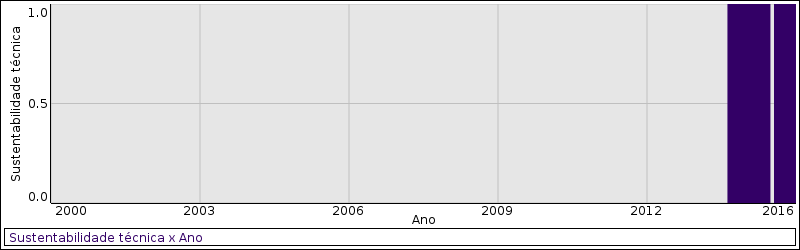
\includegraphics[scale=0.50]{imagens/softwares-charts/2ls.png}
  \caption{Sustentabilidade técnica do 2LS}
\end{figure}


\section{AccessAnalysis}
\checkmark download
\checkmark código fonte
\checkmark licença


\begin{table}[H]
\caption{Versões lançadas e número de citações ao AccessAnalysis por ano}
\centering
\begin{tabular}{| l | c | c | c | c | c |}
  \hline
  Ano & Versões & Peso da citação & Peso da autoria & Peso final & Sustentabilidade técnica \\
  \hline
        2010 & 1 & - & - & -
        &
          {\color{blue} 1.00}
        \\
\hline
            {\bf 2012}
          &
          3
          &
          1.00
          &
          0.00
          &
          1.00
          &
            {\color{blue} 1.00}
          \\
            2012
          &
          
          &
          0.10
          &
          0.00
          &
          0.10
          &
          \\
\hline
\end{tabular}
\end{table}

\begin{figure}[h]
  \center
  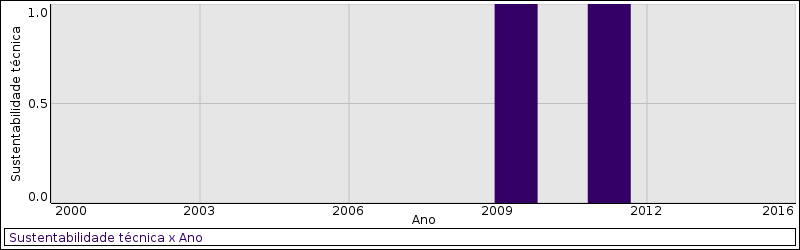
\includegraphics[scale=0.50]{imagens/softwares-charts/accessanalysis.png}
  \caption{Sustentabilidade técnica do AccessAnalysis}
\end{figure}


\section{APIExample}


\begin{table}[H]
\caption{Versões lançadas e número de citações ao APIExample por ano}
\centering
\begin{tabular}{| l | c | c | c | c | c |}
  \hline
  Ano & Versões & Peso da citação & Peso da autoria & Peso final & Sustentabilidade técnica \\
  \hline
            {\bf 2011}
          &
          
          &
          1.00
          &
          0.00
          &
          1.00
          &
            {\color{blue} 1.00}
          \\
\hline
            2013
          &
          
          &
          0.10
          &
          0.25
          &
          0.12
          &
            {\color{red} 0.12}
          \\
            2013
          &
          
          &
          0.10
          &
          0.25
          &
          0.12
          &
          \\
\hline
            2016
          &
          
          &
          0.10
          &
          0.50
          &
          0.15
          &
            {\color{red} 0.15}
          \\
\hline
\end{tabular}
\end{table}

\begin{figure}[h]
  \center
  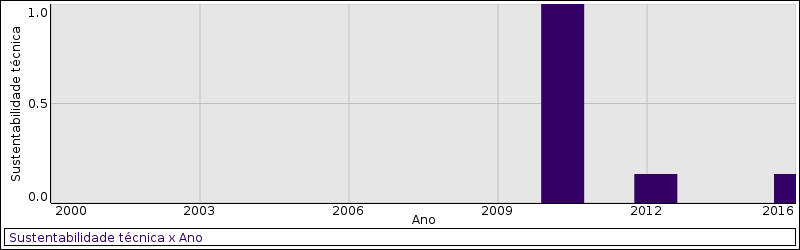
\includegraphics[scale=0.50]{imagens/softwares-charts/apiexample.png}
  \caption{Sustentabilidade técnica do APIExample}
\end{figure}


\section{BEG - Bandera environment generator}


\begin{table}[H]
\caption{Versões lançadas e número de citações ao BEG por ano}
\centering
\begin{tabular}{| l | c | c | c | c | c |}
  \hline
  Ano & Versões & Peso da citação & Peso da autoria & Peso final & Sustentabilidade técnica \\
  \hline
            {\bf 2003}
          &
          
          &
          1.00
          &
          0.00
          &
          1.00
          &
            {\color{blue} 1.00}
          \\
\hline
            2004
          &
          
          &
          0.25
          &
          0.25
          &
          0.31
          &
            {\color{red} 0.31}
          \\
\hline
            2006
          &
          
          &
          0.25
          &
          0.25
          &
          0.31
          &
            {\color{red} 0.31}
          \\
            2006
          &
          
          &
          0.10
          &
          0.25
          &
          0.12
          &
          \\
\hline
            2007
          &
          
          &
          0.25
          &
          0.10
          &
          0.28
          &
            {\color{red} 0.28}
          \\
            2007
          &
          
          &
          0.10
          &
          0.25
          &
          0.12
          &
          \\
\hline
            2010
          &
          
          &
          0.10
          &
          0.10
          &
          0.11
          &
            {\color{blue} 0.55}
          \\
            2010
          &
          
          &
          0.50
          &
          0.10
          &
          0.55
          &
          \\
\hline
            2015
          &
          
          &
          0.10
          &
          0.50
          &
          0.15
          &
            {\color{red} 0.15}
          \\
\hline
\end{tabular}
\end{table}

\begin{figure}[h]
  \center
  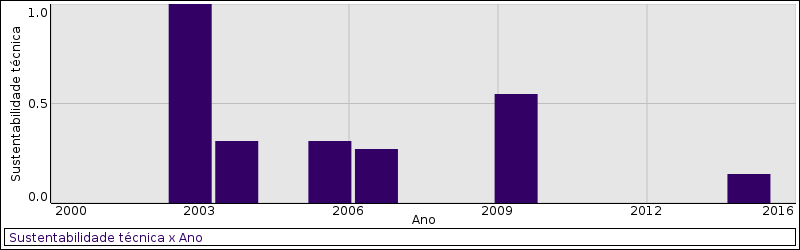
\includegraphics[scale=0.50]{imagens/softwares-charts/beg.png}
  \caption{Sustentabilidade técnica do BEG}
\end{figure}


\section{ccJava - Class-based Crosscutting Language for Java}


\begin{table}[H]
\caption{Versões lançadas e número de citações ao ccJava por ano}
\centering
\begin{tabular}{| l | c | c | c | c | c |}
  \hline
  Ano & Versões & Peso da citação & Peso da autoria & Peso final & Sustentabilidade técnica \\
  \hline
            {\bf 2007}
          &
          
          &
          1.00
          &
          0.00
          &
          1.00
          &
            {\color{blue} 1.00}
          \\
            2007
          &
          
          &
          0.10
          &
          0.00
          &
          0.10
          &
          \\
\hline
            2008
          &
          
          &
          0.50
          &
          0.00
          &
          0.50
          &
            {\color{blue} 0.50}
          \\
\hline
            2009
          &
          
          &
          0.50
          &
          0.25
          &
          0.62
          &
            {\color{blue} 0.62}
          \\
\hline
            2010
          &
          
          &
          0.50
          &
          0.10
          &
          0.55
          &
            {\color{blue} 0.55}
          \\
\hline
\end{tabular}
\end{table}

\begin{figure}[h]
  \center
  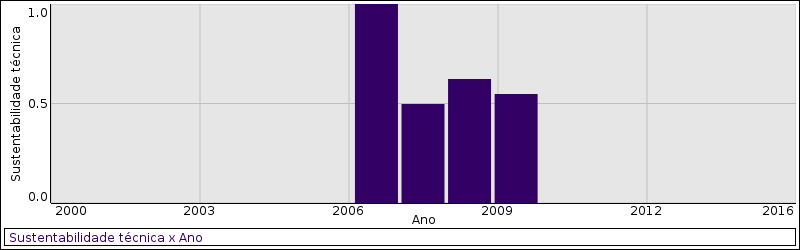
\includegraphics[scale=0.50]{imagens/softwares-charts/ccjava.png}
  \caption{Sustentabilidade técnica do ccJava}
\end{figure}


\section{CIVL - Concurrency intermediate verification language}
\checkmark download
\checkmark código fonte
\checkmark licença


\begin{table}[H]
\caption{Versões lançadas e número de citações ao CIVL por ano}
\centering
\begin{tabular}{| l | c | c | c | c | c |}
  \hline
  Ano & Versões & Peso da citação & Peso da autoria & Peso final & Sustentabilidade técnica \\
  \hline
            2015
          &
          25
          &
          0.10
          &
          0.00
          &
          0.10
          &
            {\color{blue} 1.00}
          \\
            {\bf 2015}
          &
          
          &
          1.00
          &
          0.00
          &
          1.00
          &
          \\
            2015
          &
          
          &
          0.10
          &
          0.00
          &
          0.10
          &
          \\
            2015
          &
          
          &
          0.10
          &
          0.00
          &
          0.10
          &
          \\
\hline
        2016 & 5 & - & - & -
        &
          {\color{blue} 1.00}
        \\
\hline
            2017
          &
          6
          &
          0.10
          &
          0.25
          &
          0.12
          &
            {\color{blue} 1.00}
          \\
            2017
          &
          
          &
          0.10
          &
          0.25
          &
          0.12
          &
          \\
\hline
\end{tabular}
\end{table}

\begin{figure}[h]
  \center
  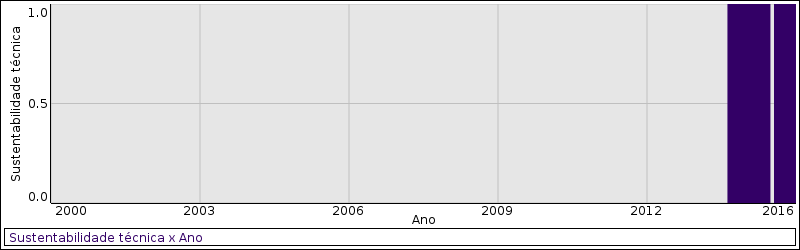
\includegraphics[scale=0.50]{imagens/softwares-charts/civl.png}
  \caption{Sustentabilidade técnica do CIVL}
\end{figure}


\section{CodeBoost}
\checkmark download
\checkmark código fonte
\checkmark licença


\begin{table}[H]
\caption{Versões lançadas e número de citações ao CodeBoost por ano}
\centering
\begin{tabular}{| l | c | c | c | c | c |}
  \hline
  Ano & Versões & Peso da citação & Peso da autoria & Peso final & Sustentabilidade técnica \\
  \hline
        2000 & 36 & - & - & -
        &
          {\color{blue} 1.00}
        \\
\hline
        2001 & 35 & - & - & -
        &
          {\color{blue} 1.00}
        \\
\hline
        2002 & 49 & - & - & -
        &
          {\color{blue} 1.00}
        \\
\hline
            {\bf 2003}
          &
          8
          &
          1.00
          &
          0.00
          &
          1.00
          &
            {\color{blue} 1.00}
          \\
            2003
          &
          
          &
          0.10
          &
          0.00
          &
          0.10
          &
          \\
\hline
        2004 & 6 & - & - & -
        &
          {\color{blue} 1.00}
        \\
\hline
            2005
          &
          
          &
          0.10
          &
          0.25
          &
          0.12
          &
            {\color{red} 0.12}
          \\
            2005
          &
          
          &
          0.10
          &
          0.10
          &
          0.11
          &
          \\
            2005
          &
          
          &
          0.10
          &
          0.25
          &
          0.12
          &
          \\
\hline
            2006
          &
          
          &
          0.10
          &
          0.25
          &
          0.12
          &
            {\color{red} 0.12}
          \\
            2006
          &
          
          &
          0.10
          &
          0.25
          &
          0.12
          &
          \\
\hline
            2008
          &
          
          &
          0.10
          &
          0.50
          &
          0.15
          &
            {\color{red} 0.15}
          \\
\hline
            2009
          &
          
          &
          0.10
          &
          0.25
          &
          0.12
          &
            {\color{red} 0.12}
          \\
\hline
            2010
          &
          
          &
          0.10
          &
          0.50
          &
          0.15
          &
            {\color{red} 0.15}
          \\
\hline
            2011
          &
          
          &
          0.10
          &
          0.50
          &
          0.15
          &
            {\color{red} 0.15}
          \\
            2011
          &
          
          &
          0.10
          &
          0.50
          &
          0.15
          &
          \\
\hline
            2012
          &
          
          &
          0.10
          &
          0.25
          &
          0.12
          &
            {\color{red} 0.12}
          \\
\hline
            2013
          &
          
          &
          0.10
          &
          0.50
          &
          0.15
          &
            {\color{red} 0.15}
          \\
\hline
            2015
          &
          
          &
          0.10
          &
          0.50
          &
          0.15
          &
            {\color{red} 0.15}
          \\
\hline
\end{tabular}
\end{table}

\begin{figure}[h]
  \center
  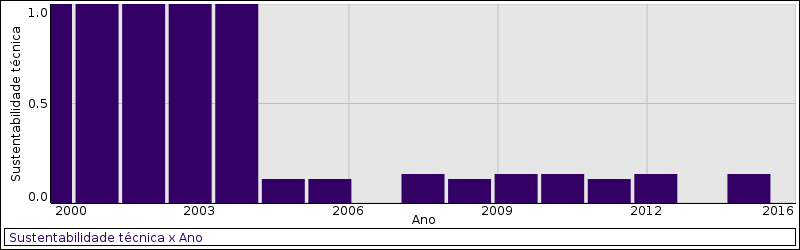
\includegraphics[scale=0.50]{imagens/softwares-charts/codeboost.png}
  \caption{Sustentabilidade técnica do CodeBoost}
\end{figure}


\section{CSL - Composite Symbolic Library}
\checkmark download
\checkmark código fonte


\begin{table}[H]
\caption{Versões lançadas e número de citações ao CSL por ano}
\centering
\begin{tabular}{| l | c | c | c | c | c |}
  \hline
  Ano & Versões & Peso da citação & Peso da autoria & Peso final & Sustentabilidade técnica \\
  \hline
            {\bf 2001}
          &
          
          &
          1.00
          &
          0.00
          &
          1.00
          &
            {\color{blue} 1.00}
          \\
\hline
            2004
          &
          
          &
          0.10
          &
          0.25
          &
          0.12
          &
            {\color{red} 0.12}
          \\
\hline
            2005
          &
          
          &
          0.10
          &
          0.50
          &
          0.15
          &
            {\color{red} 0.15}
          \\
\hline
            2006
          &
          
          &
          0.10
          &
          0.25
          &
          0.12
          &
            {\color{blue} 0.75}
          \\
            2006
          &
          
          &
          0.50
          &
          0.50
          &
          0.75
          &
          \\
\hline
            2009
          &
          
          &
          0.25
          &
          0.25
          &
          0.31
          &
            {\color{red} 0.31}
          \\
\hline
\end{tabular}
\end{table}

\begin{figure}[h]
  \center
  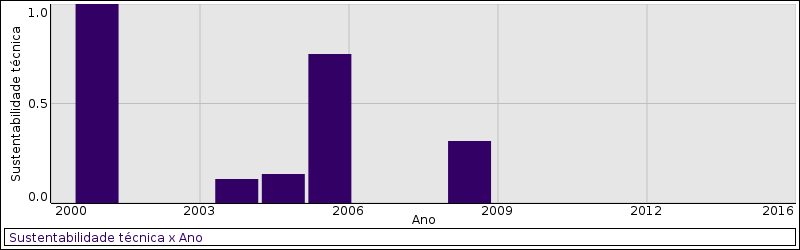
\includegraphics[scale=0.50]{imagens/softwares-charts/composite.png}
  \caption{Sustentabilidade técnica do CSL}
\end{figure}


\section{CPA+ - Configurable program analysis with dynamic precision adjustment}


\begin{table}[H]
\caption{Versões lançadas e número de citações ao CPA+ por ano}
\centering
\begin{tabular}{| l | c | c | c | c | c |}
  \hline
  Ano & Versões & Peso da citação & Peso da autoria & Peso final & Sustentabilidade técnica \\
  \hline
            {\bf 2008}
          &
          
          &
          1.00
          &
          0.00
          &
          1.00
          &
            {\color{blue} 1.00}
          \\
\hline
            2010
          &
          
          &
          0.50
          &
          0.25
          &
          0.62
          &
            {\color{blue} 0.62}
          \\
\hline
            2012
          &
          
          &
          0.50
          &
          0.10
          &
          0.55
          &
            {\color{blue} 0.55}
          \\
\hline
            2013
          &
          
          &
          0.50
            {\tiny CPA+ = CPAchecker}
          &
          0.25
          &
          0.62
          &
            {\color{blue} 0.62}
          \\
\hline
            2015
          &
          
          &
          0.50
          &
          0.25
          &
          0.62
          &
            {\color{blue} 0.62}
          \\
\hline
\end{tabular}
\end{table}

\begin{figure}[h]
  \center
  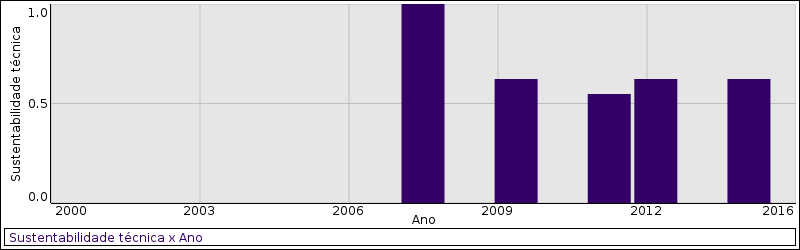
\includegraphics[scale=0.50]{imagens/softwares-charts/cpa+.png}
  \caption{Sustentabilidade técnica do CPA+}
\end{figure}


\section{CSeq}
\checkmark download
\checkmark código fonte
\checkmark licença


\begin{table}[H]
\caption{Versões lançadas e número de citações ao CSeq por ano}
\centering
\begin{tabular}{| l | c | c | c | c | c |}
  \hline
  Ano & Versões & Peso da citação & Peso da autoria & Peso final & Sustentabilidade técnica \\
  \hline
            {\bf 2013}
          &
          
          &
          1.00
          &
          0.00
          &
          1.00
          &
            {\color{blue} 1.00}
          \\
\hline
            2015
          &
          
          &
          0.50
          &
          0.00
          &
          0.50
          &
            {\color{blue} 0.50}
          \\
            2015
          &
          
          &
          0.25
          &
          0.00
          &
          0.25
          &
          \\
\hline
            2016
          &
          
          &
          0.10
          &
          0.50
          &
          0.15
          &
            {\color{red} 0.31}
          \\
            2016
          &
          
          &
          0.25
          &
          0.25
          &
          0.31
          &
          \\
\hline
\end{tabular}
\end{table}

\begin{figure}[h]
  \center
  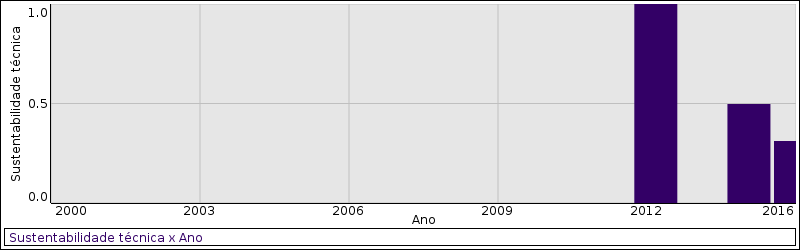
\includegraphics[scale=0.50]{imagens/softwares-charts/cseq.png}
  \caption{Sustentabilidade técnica do CSeq}
\end{figure}


\section{DDVerify}


\begin{table}[H]
\caption{Versões lançadas e número de citações ao DDVerify por ano}
\centering
\begin{tabular}{| l | c | c | c | c | c |}
  \hline
  Ano & Versões & Peso da citação & Peso da autoria & Peso final & Sustentabilidade técnica \\
  \hline
            {\bf 2007}
          &
          
          &
          1.00
          &
          0.00
          &
          1.00
          &
            {\color{blue} 1.00}
          \\
\hline
            2008
          &
          
          &
          0.10
          &
          0.10
          &
          0.11
          &
            {\color{red} 0.11}
          \\
\hline
            2014
          &
          
          &
          0.10
          &
          0.50
          &
          0.15
          &
            {\color{red} 0.15}
          \\
\hline
\end{tabular}
\end{table}

\begin{figure}[h]
  \center
  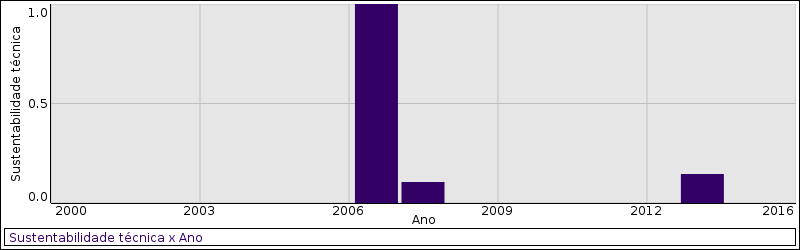
\includegraphics[scale=0.50]{imagens/softwares-charts/ddverify.png}
  \caption{Sustentabilidade técnica do DDVerify}
\end{figure}


\section{Derailer}
\checkmark download
\checkmark código fonte
\checkmark licença


\begin{table}[H]
\caption{Versões lançadas e número de citações ao Derailer por ano}
\centering
\begin{tabular}{| l | c | c | c | c | c |}
  \hline
  Ano & Versões & Peso da citação & Peso da autoria & Peso final & Sustentabilidade técnica \\
  \hline
        2013 & 1 & - & - & -
        &
          {\color{blue} 1.00}
        \\
\hline
            {\bf 2014}
          &
          1
          &
          1.00
          &
          0.00
          &
          1.00
          &
            {\color{blue} 1.00}
          \\
\hline
            2016
          &
          
          &
          0.10
            {\tiny SPACE}
          &
          0.10
          &
          0.11
          &
            {\color{red} 0.11}
          \\
\hline
\end{tabular}
\end{table}

\begin{figure}[h]
  \center
  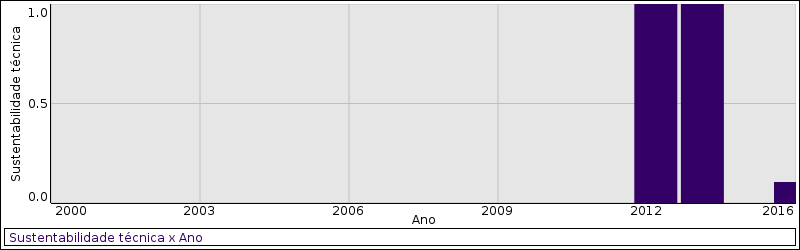
\includegraphics[scale=0.50]{imagens/softwares-charts/derailer.png}
  \caption{Sustentabilidade técnica do Derailer}
\end{figure}


\section{Diagnosys}


\begin{table}[H]
\caption{Versões lançadas e número de citações ao Diagnosys por ano}
\centering
\begin{tabular}{| l | c | c | c | c | c |}
  \hline
  Ano & Versões & Peso da citação & Peso da autoria & Peso final & Sustentabilidade técnica \\
  \hline
            {\bf 2012}
          &
          
          &
          1.00
          &
          0.00
          &
          1.00
          &
            {\color{blue} 1.00}
          \\
\hline
\end{tabular}
\end{table}

\begin{figure}[h]
  \center
  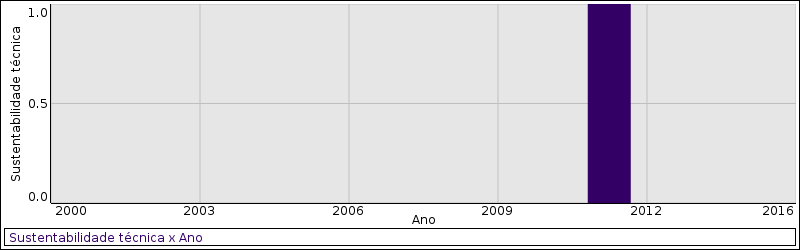
\includegraphics[scale=0.50]{imagens/softwares-charts/diagnosys.png}
  \caption{Sustentabilidade técnica do Diagnosys}
\end{figure}


\section{DOMPLETION}
\checkmark download
\checkmark código fonte


\begin{table}[H]
\caption{Versões lançadas e número de citações ao DOMPLETION por ano}
\centering
\begin{tabular}{| l | c | c | c | c | c |}
  \hline
  Ano & Versões & Peso da citação & Peso da autoria & Peso final & Sustentabilidade técnica \\
  \hline
            {\bf 2014}
          &
          
          &
          1.00
          &
          0.00
          &
          1.00
          &
            {\color{blue} 1.00}
          \\
\hline
            2015
          &
          
          &
          0.10
          &
          0.10
          &
          0.11
          &
            {\color{red} 0.11}
          \\
\hline
\end{tabular}
\end{table}

\begin{figure}[h]
  \center
  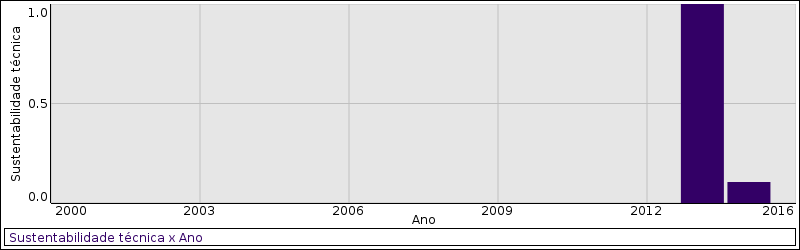
\includegraphics[scale=0.50]{imagens/softwares-charts/dompletion.png}
  \caption{Sustentabilidade técnica do DOMPLETION}
\end{figure}


\section{DRC - Dangling Reference Checker}


\begin{table}[H]
\caption{Versões lançadas e número de citações ao DRC por ano}
\centering
\begin{tabular}{| l | c | c | c | c | c |}
  \hline
  Ano & Versões & Peso da citação & Peso da autoria & Peso final & Sustentabilidade técnica \\
  \hline
            2013
          &
          
          &
          0.10
          &
          0.00
          &
          0.10
          &
            {\color{blue} 1.00}
          \\
            {\bf 2013}
          &
          
          &
          1.00
          &
          0.00
          &
          1.00
          &
          \\
\hline
            2014
          &
          
          &
          0.10
          &
          0.25
          &
          0.12
          &
            {\color{red} 0.15}
          \\
            2014
          &
          
          &
          0.10
          &
          0.50
          &
          0.15
          &
          \\
\hline
            2015
          &
          
          &
          0.10
          &
          0.10
          &
          0.11
          &
            {\color{red} 0.11}
          \\
\hline
\end{tabular}
\end{table}

\begin{figure}[h]
  \center
  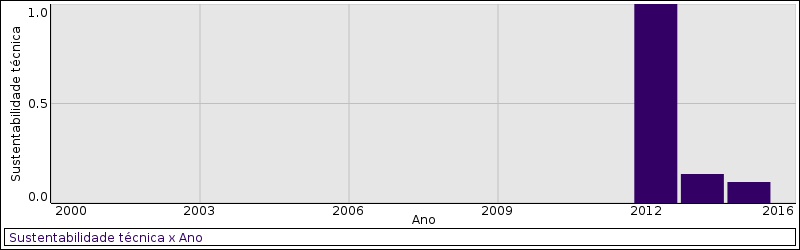
\includegraphics[scale=0.50]{imagens/softwares-charts/drc.png}
  \caption{Sustentabilidade técnica do DRC}
\end{figure}


\section{e-munity}
\checkmark download
\checkmark código fonte


\begin{table}[H]
\caption{Versões lançadas e número de citações ao e-munity por ano}
\centering
\begin{tabular}{| l | c | c | c | c | c |}
  \hline
  Ano & Versões & Peso da citação & Peso da autoria & Peso final & Sustentabilidade técnica \\
  \hline
            {\bf 2014}
          &
          
          &
          1.00
          &
          0.00
          &
          1.00
          &
            {\color{blue} 1.00}
          \\
\hline
\end{tabular}
\end{table}

\begin{figure}[h]
  \center
  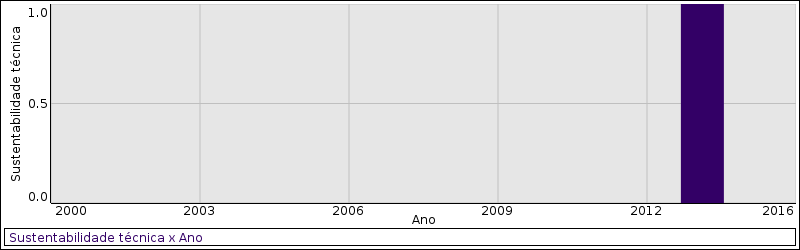
\includegraphics[scale=0.50]{imagens/softwares-charts/e-munity.png}
  \caption{Sustentabilidade técnica do e-munity}
\end{figure}


\section{EJB Interceptor Analyzer}
\checkmark download
\checkmark código fonte


\begin{table}[H]
\caption{Versões lançadas e número de citações ao EJB Interceptor Analyzer por ano}
\centering
\begin{tabular}{| l | c | c | c | c | c |}
  \hline
  Ano & Versões & Peso da citação & Peso da autoria & Peso final & Sustentabilidade técnica \\
  \hline
            {\bf 2011}
          &
          
          &
          1.00
          &
          0.00
          &
          1.00
          &
            {\color{blue} 1.00}
          \\
\hline
            2013
          &
          
          &
          0.10
            {\tiny I2SD = EJB}
          &
          0.25
          &
          0.12
          &
            {\color{red} 0.12}
          \\
\hline
            2017
          &
          
          &
          0.25
          &
          0.50
          &
          0.38
          &
            {\color{red} 0.38}
          \\
\hline
\end{tabular}
\end{table}

\begin{figure}[h]
  \center
  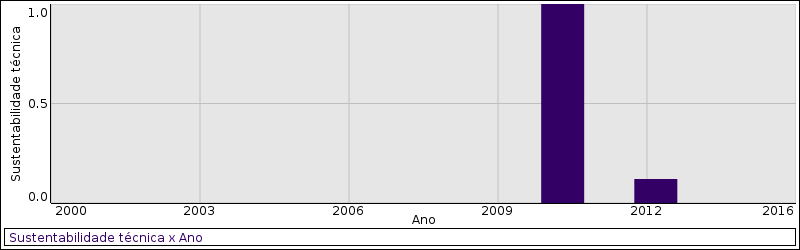
\includegraphics[scale=0.50]{imagens/softwares-charts/ejb.png}
  \caption{Sustentabilidade técnica do EJB Interceptor Analyzer}
\end{figure}


\section{Error Prone}
\checkmark download
\checkmark código fonte
\checkmark licença


\begin{table}[H]
\caption{Versões lançadas e número de citações ao Error Prone por ano}
\centering
\begin{tabular}{| l | c | c | c | c | c |}
  \hline
  Ano & Versões & Peso da citação & Peso da autoria & Peso final & Sustentabilidade técnica \\
  \hline
            {\bf 2012}
          &
          
          &
          1.00
          &
          0.00
          &
          1.00
          &
            {\color{blue} 1.00}
          \\
\hline
            2015
          &
          8
          &
          0.25
          &
          0.50
          &
          0.38
          &
            {\color{blue} 1.00}
          \\
\hline
        2016 & 8 & - & - & -
        &
          {\color{blue} 1.00}
        \\
\hline
        2017 & 6 & - & - & -
        &
          {\color{blue} 1.00}
        \\
\hline
\end{tabular}
\end{table}

\begin{figure}[h]
  \center
  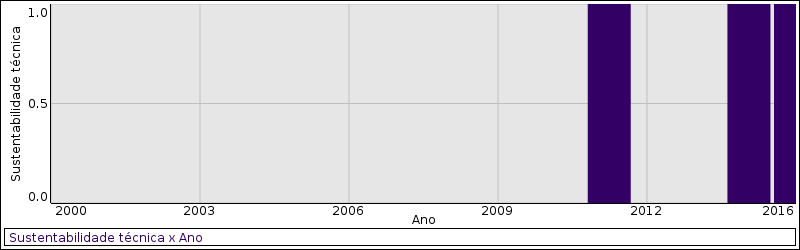
\includegraphics[scale=0.50]{imagens/softwares-charts/error-prone.png}
  \caption{Sustentabilidade técnica do Error Prone}
\end{figure}


\section{ESBMC - Efficient SMT-Based Context-Bounded Model Checker}


\begin{table}[H]
\caption{Versões lançadas e número de citações ao ESBMC por ano}
\centering
\begin{tabular}{| l | c | c | c | c | c |}
  \hline
  Ano & Versões & Peso da citação & Peso da autoria & Peso final & Sustentabilidade técnica \\
  \hline
            {\bf 2009}
          &
          
          &
          1.00
          &
          0.00
          &
          1.00
          &
            {\color{blue} 1.00}
          \\
\hline
            2010
          &
          
          &
          0.25
          &
          0.10
          &
          0.28
          &
            {\color{red} 0.28}
          \\
\hline
            2011
          &
          
          &
          0.25
          &
          0.50
          &
          0.38
          &
            {\color{blue} 0.62}
          \\
            2011
          &
          
          &
          0.50
          &
          0.25
          &
          0.62
          &
          \\
            2011
          &
          
          &
          0.25
          &
          0.25
          &
          0.31
          &
          \\
\hline
            2012
          &
          
          &
          0.25
          &
          0.50
          &
          0.38
          &
            {\color{red} 0.38}
          \\
            2012
          &
          
          &
          0.25
          &
          0.50
          &
          0.38
          &
          \\
\hline
            2013
          &
          
          &
          0.25
          &
          0.25
          &
          0.31
          &
            {\color{blue} 0.62}
          \\
            2013
          &
          
          &
          0.10
          &
          0.25
          &
          0.12
          &
          \\
            2013
          &
          
          &
          0.10
          &
          0.25
          &
          0.12
          &
          \\
            2013
          &
          
          &
          0.50
          &
          0.25
          &
          0.62
          &
          \\
            2013
          &
          
          &
          0.25
          &
          0.25
          &
          0.31
          &
          \\
            2013
          &
          
          &
          0.25
          &
          0.25
          &
          0.31
          &
          \\
\hline
            2014
          &
          
          &
          0.50
          &
          0.25
          &
          0.62
          &
            {\color{blue} 0.62}
          \\
            2014
          &
          
          &
          0.25
          &
          0.25
          &
          0.31
          &
          \\
            2014
          &
          
          &
          0.10
          &
          0.50
          &
          0.15
          &
          \\
            2014
          &
          
          &
          0.25
          &
          0.25
          &
          0.31
          &
          \\
            2014
          &
          
          &
          0.25
          &
          0.25
          &
          0.31
          &
          \\
            2014
          &
          
          &
          0.25
          &
          0.25
          &
          0.31
          &
          \\
\hline
            2015
          &
          
          &
          0.50
          &
          0.25
          &
          0.62
          &
            {\color{blue} 0.62}
          \\
            2015
          &
          
          &
          0.10
          &
          0.25
          &
          0.12
          &
          \\
            2015
          &
          
          &
          0.50
          &
          0.25
          &
          0.62
          &
          \\
            2015
          &
          
          &
          0.25
          &
          0.25
          &
          0.31
          &
          \\
            2015
          &
          
          &
          0.10
          &
          0.25
          &
          0.12
          &
          \\
            2015
          &
          
          &
          0.50
          &
          0.25
          &
          0.62
          &
          \\
            2015
          &
          
          &
          0.25
          &
          0.25
          &
          0.31
          &
          \\
            2015
          &
          
          &
          0.10
          &
          0.25
          &
          0.12
          &
          \\
\hline
            2016
          &
          
          &
          0.25
          &
          0.25
          &
          0.31
          &
            {\color{blue} 0.62}
          \\
            2016
          &
          
          &
          0.10
          &
          0.25
          &
          0.12
          &
          \\
            2016
          &
          
          &
          0.10
          &
          0.50
          &
          0.15
          &
          \\
            2016
          &
          
          &
          0.25
          &
          0.25
          &
          0.31
          &
          \\
            2016
          &
          
          &
          0.10
          &
          0.25
          &
          0.12
          &
          \\
            2016
          &
          
          &
          0.10
          &
          0.25
          &
          0.12
          &
          \\
            2016
          &
          
          &
          0.10
          &
          0.25
          &
          0.12
          &
          \\
            2016
          &
          
          &
          0.10
          &
          0.25
          &
          0.12
          &
          \\
            2016
          &
          
          &
          0.25
          &
          0.25
          &
          0.31
          &
          \\
            2016
          &
          
          &
          0.10
          &
          0.25
          &
          0.12
          &
          \\
            2016
          &
          
          &
          0.50
          &
          0.25
          &
          0.62
          &
          \\
\hline
            2017
          &
          
          &
          0.25
          &
          0.25
          &
          0.31
          &
            {\color{red} 0.31}
          \\
            2017
          &
          
          &
          0.25
          &
          0.25
          &
          0.31
          &
          \\
            2017
          &
          
          &
          0.10
          &
          0.25
          &
          0.12
          &
          \\
            2017
          &
          
          &
          0.10
          &
          0.25
          &
          0.12
          &
          \\
\hline
\end{tabular}
\end{table}

\begin{figure}[h]
  \center
  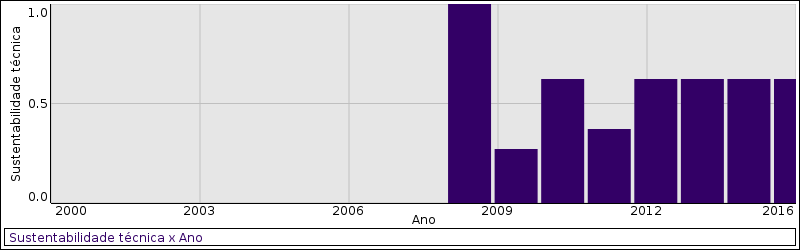
\includegraphics[scale=0.50]{imagens/softwares-charts/esbmc.png}
  \caption{Sustentabilidade técnica do ESBMC}
\end{figure}


\section{ETXL}


\begin{table}[H]
\caption{Versões lançadas e número de citações ao ETXL por ano}
\centering
\begin{tabular}{| l | c | c | c | c | c |}
  \hline
  Ano & Versões & Peso da citação & Peso da autoria & Peso final & Sustentabilidade técnica \\
  \hline
            {\bf 2006}
          &
          
          &
          1.00
          &
          0.00
          &
          1.00
          &
            {\color{blue} 1.00}
          \\
\hline
\end{tabular}
\end{table}

\begin{figure}[h]
  \center
  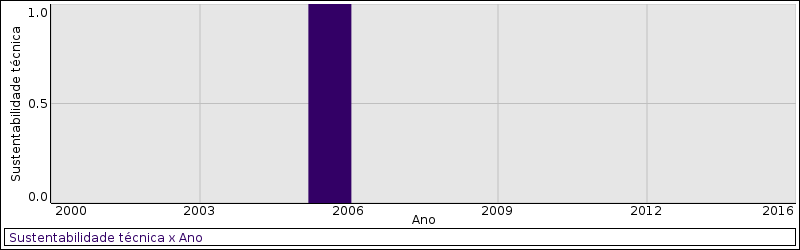
\includegraphics[scale=0.50]{imagens/softwares-charts/etxl.png}
  \caption{Sustentabilidade técnica do ETXL}
\end{figure}


\section{FaultBuster}
\checkmark download
\checkmark licença


\begin{table}[H]
\caption{Versões lançadas e número de citações ao FaultBuster por ano}
\centering
\begin{tabular}{| l | c | c | c | c | c |}
  \hline
  Ano & Versões & Peso da citação & Peso da autoria & Peso final & Sustentabilidade técnica \\
  \hline
            {\bf 2015}
          &
          
          &
          1.00
          &
          0.00
          &
          1.00
          &
            {\color{blue} 1.00}
          \\
\hline
\end{tabular}
\end{table}

\begin{figure}[h]
  \center
  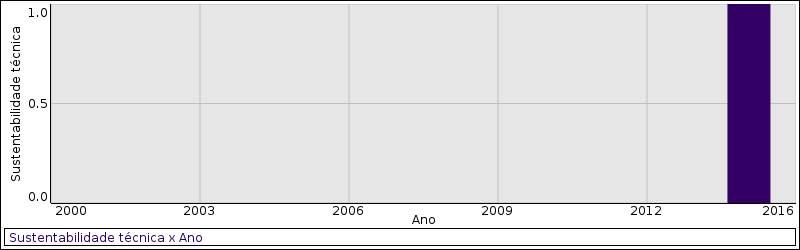
\includegraphics[scale=0.50]{imagens/softwares-charts/faultbuster.png}
  \caption{Sustentabilidade técnica do FaultBuster}
\end{figure}


\section{Flowgen}
\checkmark download
\checkmark código fonte
\checkmark licença


\begin{table}[H]
\caption{Versões lançadas e número de citações ao Flowgen por ano}
\centering
\begin{tabular}{| l | c | c | c | c | c |}
  \hline
  Ano & Versões & Peso da citação & Peso da autoria & Peso final & Sustentabilidade técnica \\
  \hline
            {\bf 2014}
          &
          
          &
          1.00
          &
          0.00
          &
          1.00
          &
            {\color{blue} 1.00}
          \\
\hline
            2015
          &
          
          &
          0.10
          &
          0.50
          &
          0.15
          &
            {\color{red} 0.15}
          \\
\hline
            2016
          &
          
          &
          0.10
          &
          0.50
          &
          0.15
          &
            {\color{red} 0.15}
          \\
\hline
\end{tabular}
\end{table}

\begin{figure}[h]
  \center
  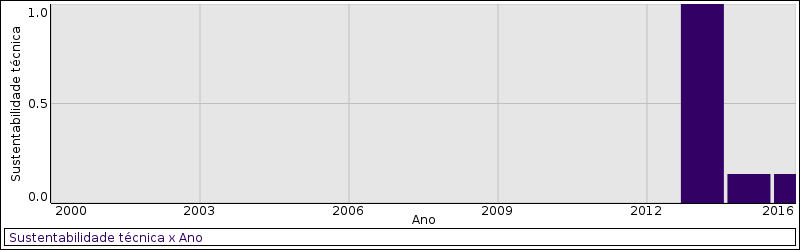
\includegraphics[scale=0.50]{imagens/softwares-charts/flowgen.png}
  \caption{Sustentabilidade técnica do Flowgen}
\end{figure}


\section{GRT - Guided Random Testing}


\begin{table}[H]
\caption{Versões lançadas e número de citações ao GRT por ano}
\centering
\begin{tabular}{| l | c | c | c | c | c |}
  \hline
  Ano & Versões & Peso da citação & Peso da autoria & Peso final & Sustentabilidade técnica \\
  \hline
            2014
          &
          
          &
          0.10
            {\tiny BGRT}
          &
          0.00
          &
          0.10
          &
            {\color{red} 0.10}
          \\
\hline
            2015
          &
          
          &
          0.10
            {\tiny 1º no SBST '15}
          &
          0.50
          &
          0.15
          &
            {\color{blue} 0.75}
          \\
            {\bf 2015}
          &
          
          &
          0.50
          &
          0.50
          &
          0.75
          &
          \\
            {\bf 2015}
          &
          
          &
          0.50
          &
          0.50
          &
          0.75
          &
          \\
\hline
            2016
          &
          
          &
          0.25
          &
          0.10
          &
          0.28
          &
            {\color{blue} 0.62}
          \\
            2016
          &
          
          &
          0.50
          &
          0.25
          &
          0.62
          &
          \\
\hline
            2017
          &
          
          &
          0.10
          &
          0.50
          &
          0.15
          &
            {\color{red} 0.31}
          \\
            2017
          &
          
          &
          0.25
          &
          0.25
          &
          0.31
          &
          \\
            2017
          &
          
          &
          0.10
          &
          0.25
          &
          0.12
          &
          \\
\hline
\end{tabular}
\end{table}

\begin{figure}[h]
  \center
  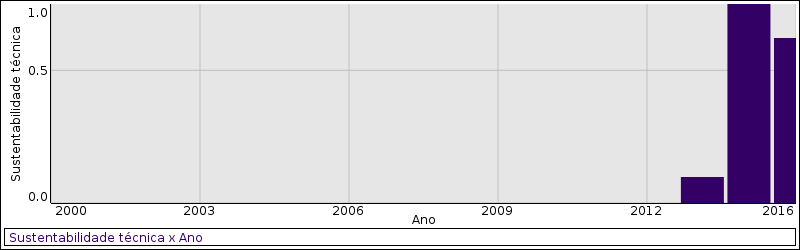
\includegraphics[scale=0.50]{imagens/softwares-charts/grt.png}
  \caption{Sustentabilidade técnica do GRT}
\end{figure}


\section{GUIZMO}
\checkmark download
\checkmark código fonte
\checkmark licença


\begin{table}[H]
\caption{Versões lançadas e número de citações ao GUIZMO por ano}
\centering
\begin{tabular}{| l | c | c | c | c | c |}
  \hline
  Ano & Versões & Peso da citação & Peso da autoria & Peso final & Sustentabilidade técnica \\
  \hline
            {\bf 2010}
          &
          
          &
          1.00
          &
          0.00
          &
          1.00
          &
            {\color{blue} 1.00}
          \\
\hline
\end{tabular}
\end{table}

\begin{figure}[h]
  \center
  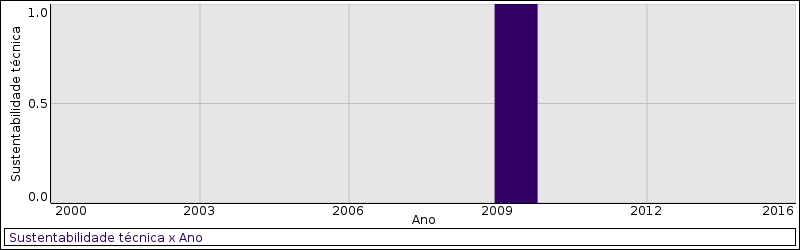
\includegraphics[scale=0.50]{imagens/softwares-charts/guizmo.png}
  \caption{Sustentabilidade técnica do GUIZMO}
\end{figure}


\section{GumTree}
\checkmark download
\checkmark código fonte
\checkmark licença


\begin{table}[H]
\caption{Versões lançadas e número de citações ao GumTree por ano}
\centering
\begin{tabular}{| l | c | c | c | c | c |}
  \hline
  Ano & Versões & Peso da citação & Peso da autoria & Peso final & Sustentabilidade técnica \\
  \hline
        2013 & 1 & - & - & -
        &
          {\color{blue} 1.00}
        \\
\hline
            {\bf 2014}
          &
          
          &
          1.00
          &
          0.00
          &
          1.00
          &
            {\color{blue} 1.00}
          \\
\hline
            2015
          &
          2
          &
          0.10
          &
          0.50
          &
          0.15
          &
            {\color{blue} 1.00}
          \\
            2015
          &
          
          &
          0.25
          &
          0.50
          &
          0.38
          &
          \\
\hline
            2016
          &
          
          &
          0.25
          &
          0.50
          &
          0.38
          &
            {\color{red} 0.38}
          \\
            2016
          &
          
          &
          0.10
          &
          0.50
          &
          0.15
          &
          \\
            2016
          &
          
          &
          0.25
          &
          0.50
          &
          0.38
          &
          \\
            2016
          &
          
          &
          0.25
          &
          0.50
          &
          0.38
          &
          \\
            2016
          &
          
          &
          0.25
          &
          0.50
          &
          0.38
          &
          \\
            2016
          &
          
          &
          0.25
          &
          0.50
          &
          0.38
          &
          \\
\hline
            2017
          &
          
          &
          0.25
          &
          0.25
          &
          0.31
          &
            {\color{blue} 0.62}
          \\
            2017
          &
          
          &
          0.10
          &
          0.25
          &
          0.12
          &
          \\
            2017
          &
          
          &
          0.50
          &
          0.25
          &
          0.62
          &
          \\
            2017
          &
          
          &
          0.10
          &
          0.25
          &
          0.12
          &
          \\
            2017
          &
          
          &
          0.25
          &
          0.25
          &
          0.31
          &
          \\
            2017
          &
          
          &
          0.10
          &
          0.25
          &
          0.12
          &
          \\
            2017
          &
          
          &
          0.25
          &
          0.25
          &
          0.31
          &
          \\
            2017
          &
          
          &
          0.25
          &
          0.25
          &
          0.31
          &
          \\
            2017
          &
          
          &
          0.25
          &
          0.25
          &
          0.31
          &
          \\
\hline
\end{tabular}
\end{table}

\begin{figure}[h]
  \center
  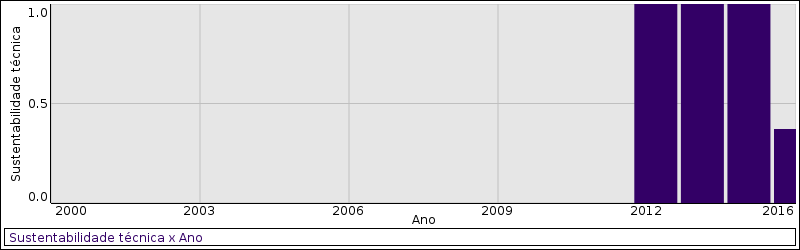
\includegraphics[scale=0.50]{imagens/softwares-charts/gumtree.png}
  \caption{Sustentabilidade técnica do GumTree}
\end{figure}


\section{HUSACCT - HU Software Architecture Compliance Checking Tool}
\checkmark download
\checkmark código fonte
\checkmark licença


\begin{table}[H]
\caption{Versões lançadas e número de citações ao HUSACCT por ano}
\centering
\begin{tabular}{| l | c | c | c | c | c |}
  \hline
  Ano & Versões & Peso da citação & Peso da autoria & Peso final & Sustentabilidade técnica \\
  \hline
        2013 & 3 & - & - & -
        &
          {\color{blue} 1.00}
        \\
\hline
            2014
          &
          7
          &
          0.10
          &
          0.00
          &
          0.10
          &
            {\color{blue} 1.00}
          \\
            {\bf 2014}
          &
          
          &
          1.00
          &
          0.00
          &
          1.00
          &
          \\
\hline
            2015
          &
          6
          &
          0.25
          &
          0.25
          &
          0.31
          &
            {\color{blue} 1.00}
          \\
\hline
            2016
          &
          3
          &
          0.10
          &
          0.25
          &
          0.12
          &
            {\color{blue} 1.00}
          \\
            2016
          &
          
          &
          0.10
          &
          0.25
          &
          0.12
          &
          \\
            2016
          &
          
          &
          1.00
          &
          0.25
          &
          1.00
          &
          \\
            2016
          &
          
          &
          0.25
          &
          0.25
          &
          0.31
          &
          \\
\hline
        2017 & 3 & - & - & -
        &
          {\color{blue} 1.00}
        \\
\hline
\end{tabular}
\end{table}

\begin{figure}[h]
  \center
  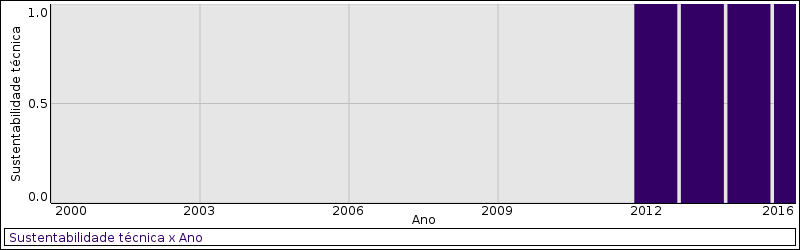
\includegraphics[scale=0.50]{imagens/softwares-charts/husacct.png}
  \caption{Sustentabilidade técnica do HUSACCT}
\end{figure}


\section{Indus}
\checkmark download
\checkmark código fonte
\checkmark licença


\begin{table}[H]
\caption{Versões lançadas e número de citações ao Indus por ano}
\centering
\begin{tabular}{| l | c | c | c | c | c |}
  \hline
  Ano & Versões & Peso da citação & Peso da autoria & Peso final & Sustentabilidade técnica \\
  \hline
        2005 & 13 & - & - & -
        &
          {\color{blue} 1.00}
        \\
\hline
            {\bf 2006}
          &
          14
          &
          1.00
          &
          0.00
          &
          1.00
          &
            {\color{blue} 1.00}
          \\
\hline
        2007 & 6 & - & - & -
        &
          {\color{blue} 1.00}
        \\
\hline
            2009
          &
          2
          &
          0.25
          &
          0.50
          &
          0.38
          &
            {\color{blue} 1.00}
          \\
\hline
        2010 & 1 & - & - & -
        &
          {\color{blue} 1.00}
        \\
\hline
            2012
          &
          
          &
          0.25
          &
          0.25
          &
          0.31
          &
            {\color{red} 0.31}
          \\
            2012
          &
          
          &
          0.25
          &
          0.25
          &
          0.31
          &
          \\
\hline
\end{tabular}
\end{table}

\begin{figure}[h]
  \center
  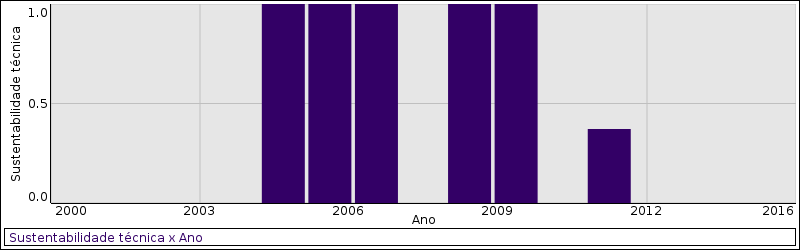
\includegraphics[scale=0.50]{imagens/softwares-charts/indus.png}
  \caption{Sustentabilidade técnica do Indus}
\end{figure}


\section{JastAdd}
\checkmark download
\checkmark código fonte
\checkmark licença


\begin{table}[H]
\caption{Versões lançadas e número de citações ao JastAdd por ano}
\centering
\begin{tabular}{| l | c | c | c | c | c |}
  \hline
  Ano & Versões & Peso da citação & Peso da autoria & Peso final & Sustentabilidade técnica \\
  \hline
            2003
          &
          
          &
          0.10
          &
          0.00
          &
          0.10
          &
            {\color{red} 0.10}
          \\
\hline
            2005
          &
          
          &
          0.10
          &
          0.50
          &
          0.15
          &
            {\color{red} 0.38}
          \\
            2005
          &
          
          &
          0.25
          &
          0.50
          &
          0.38
          &
          \\
            2005
          &
          
          &
          0.10
          &
          0.50
          &
          0.15
          &
          \\
            2005
          &
          
          &
          0.10
          &
          0.50
          &
          0.15
          &
          \\
\hline
            2006
          &
          
          &
          0.10
          &
          0.50
          &
          0.15
          &
            {\color{red} 0.31}
          \\
            2006
          &
          
          &
          0.10
          &
          0.25
          &
          0.12
          &
          \\
            2006
          &
          
          &
          0.25
          &
          0.25
          &
          0.31
          &
          \\
\hline
            2007
          &
          
          &
          0.10
          &
          0.25
          &
          0.12
          &
            {\color{blue} 1.00}
          \\
            {\bf 2007}
          &
          
          &
          1.00
          &
          0.25
          &
          1.00
          &
          \\
            2007
          &
          
          &
          0.25
          &
          0.25
          &
          0.31
          &
          \\
            2007
          &
          
          &
          0.25
          &
          0.25
          &
          0.31
          &
          \\
\hline
            2008
          &
          
          &
          0.10
          &
          0.25
          &
          0.12
          &
            {\color{blue} 0.62}
          \\
            2008
          &
          
          &
          0.10
          &
          0.25
          &
          0.12
          &
          \\
            2008
          &
          
          &
          0.25
          &
          0.25
          &
          0.31
          &
          \\
            2008
          &
          
          &
          0.50
          &
          0.25
          &
          0.62
          &
          \\
\hline
            2009
          &
          
          &
          0.10
          &
          0.25
          &
          0.12
          &
            {\color{red} 0.15}
          \\
            2009
          &
          
          &
          0.10
          &
          0.50
          &
          0.15
          &
          \\
\hline
            2010
          &
          
          &
          0.10
          &
          0.25
          &
          0.12
          &
            {\color{blue} 0.62}
          \\
            2010
          &
          
          &
          0.25
          &
          0.25
          &
          0.31
          &
          \\
            2010
          &
          
          &
          0.10
          &
          0.25
          &
          0.12
          &
          \\
            2010
          &
          
          &
          0.10
          &
          0.25
          &
          0.12
          &
          \\
            2010
          &
          
          &
          0.50
          &
          0.25
          &
          0.62
          &
          \\
            2010
          &
          
          &
          0.10
          &
          0.25
          &
          0.12
          &
          \\
\hline
            2011
          &
          1
          &
          0.25
          &
          0.25
          &
          0.31
          &
            {\color{blue} 1.00}
          \\
            2011
          &
          
          &
          0.10
          &
          0.50
          &
          0.15
          &
          \\
            2011
          &
          
          &
          0.10
          &
          0.50
          &
          0.15
          &
          \\
\hline
            2012
          &
          3
          &
          0.25
          &
          0.25
          &
          0.31
          &
            {\color{blue} 1.00}
          \\
            2012
          &
          
          &
          0.25
          &
          0.25
          &
          0.31
          &
          \\
            2012
          &
          
          &
          0.25
          &
          0.25
          &
          0.31
          &
          \\
            2012
          &
          
          &
          0.10
          &
          0.25
          &
          0.12
          &
          \\
\hline
            2013
          &
          9
          &
          0.25
          &
          0.25
          &
          0.31
          &
            {\color{blue} 1.00}
          \\
            2013
          &
          
          &
          0.25
          &
          0.25
          &
          0.31
          &
          \\
            2013
          &
          
          &
          0.50
          &
          0.25
          &
          0.62
          &
          \\
\hline
            2014
          &
          4
          &
          0.10
          &
          0.25
          &
          0.12
          &
            {\color{blue} 1.00}
          \\
            2014
          &
          
          &
          0.25
          &
          0.10
          &
          0.28
          &
          \\
\hline
            2015
          &
          3
          &
          0.10
          &
          0.25
          &
          0.12
          &
            {\color{blue} 1.00}
          \\
            2015
          &
          
          &
          0.10
          &
          0.25
          &
          0.12
          &
          \\
\hline
            2016
          &
          3
          &
          0.25
          &
          0.25
          &
          0.31
          &
            {\color{blue} 1.00}
          \\
            2016
          &
          
          &
          0.10
          &
          0.25
          &
          0.12
          &
          \\
            2016
          &
          
          &
          0.25
          &
          0.25
          &
          0.31
          &
          \\
\hline
            2017
          &
          1
          &
          0.10
          &
          0.50
          &
          0.15
          &
            {\color{blue} 1.00}
          \\
            2017
          &
          
          &
          0.10
          &
          0.50
          &
          0.15
          &
          \\
\hline
\end{tabular}
\end{table}

\begin{figure}[h]
  \center
  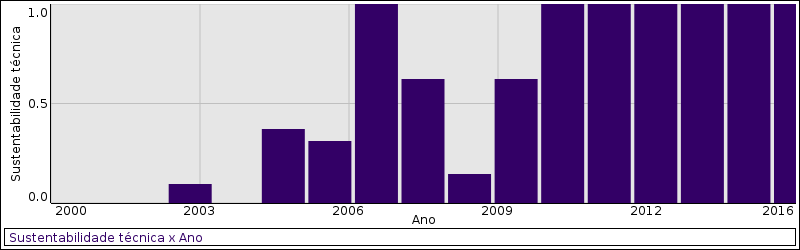
\includegraphics[scale=0.50]{imagens/softwares-charts/jastadd.png}
  \caption{Sustentabilidade técnica do JastAdd}
\end{figure}


\section{JFlow}
\checkmark download
\checkmark código fonte
\checkmark licença


\begin{table}[H]
\caption{Versões lançadas e número de citações ao JFlow por ano}
\centering
\begin{tabular}{| l | c | c | c | c | c |}
  \hline
  Ano & Versões & Peso da citação & Peso da autoria & Peso final & Sustentabilidade técnica \\
  \hline
            2006
          &
          
          &
          0.10
          &
          0.00
          &
          0.10
          &
            {\color{red} 0.10}
          \\
            2006
          &
          
          &
          0.10
          &
          0.00
          &
          0.10
          &
          \\
\hline
            2007
          &
          
          &
          0.25
          &
          0.25
          &
          0.31
          &
            {\color{red} 0.31}
          \\
\hline
            2011
          &
          
          &
          0.10
          &
          0.50
          &
          0.15
          &
            {\color{red} 0.15}
          \\
            2011
          &
          
          &
          0.10
          &
          0.50
          &
          0.15
          &
          \\
\hline
        2012 & 5 & - & - & -
        &
          {\color{blue} 1.00}
        \\
\hline
            {\bf 2013}
          &
          
          &
          1.00
          &
          0.50
          &
          1.00
          &
            {\color{blue} 1.00}
          \\
\hline
            2014
          &
          
          &
          0.10
          &
          0.50
          &
          0.15
          &
            {\color{red} 0.15}
          \\
\hline
\end{tabular}
\end{table}

\begin{figure}[h]
  \center
  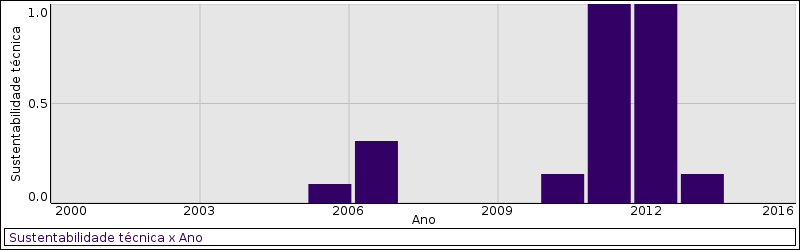
\includegraphics[scale=0.50]{imagens/softwares-charts/jflow.png}
  \caption{Sustentabilidade técnica do JFlow}
\end{figure}


\section{JstereoCode}


\begin{table}[H]
\caption{Versões lançadas e número de citações ao JstereoCode por ano}
\centering
\begin{tabular}{| l | c | c | c | c | c |}
  \hline
  Ano & Versões & Peso da citação & Peso da autoria & Peso final & Sustentabilidade técnica \\
  \hline
            {\bf 2012}
          &
          
          &
          1.00
          &
          0.00
          &
          1.00
          &
            {\color{blue} 1.00}
          \\
\hline
            2013
          &
          
          &
          0.25
          &
          0.00
          &
          0.25
          &
            {\color{red} 0.25}
          \\
            2013
          &
          
          &
          0.25
          &
          0.00
          &
          0.25
          &
          \\
            2013
          &
          
          &
          0.10
          &
          0.00
          &
          0.10
          &
          \\
\hline
            2015
          &
          
          &
          0.25
          &
          0.25
          &
          0.31
          &
            {\color{red} 0.31}
          \\
            2015
          &
          
          &
          0.25
          &
          0.25
          &
          0.31
          &
          \\
\hline
            2016
          &
          
          &
          0.25
          &
          0.50
          &
          0.38
          &
            {\color{red} 0.38}
          \\
\hline
            2017
          &
          
          &
          0.10
          &
          0.50
          &
          0.15
          &
            {\color{red} 0.15}
          \\
\hline
\end{tabular}
\end{table}

\begin{figure}[h]
  \center
  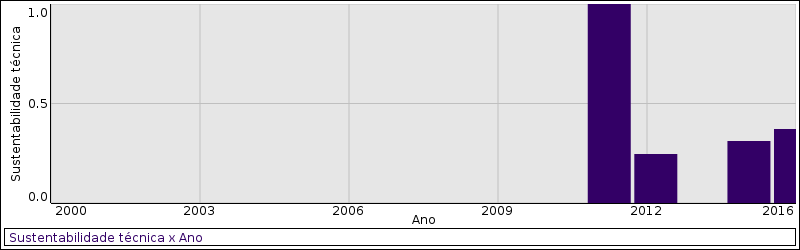
\includegraphics[scale=0.50]{imagens/softwares-charts/jstereocode.png}
  \caption{Sustentabilidade técnica do JstereoCode}
\end{figure}


\section{Jtop}
\checkmark licença


\begin{table}[H]
\caption{Versões lançadas e número de citações ao Jtop por ano}
\centering
\begin{tabular}{| l | c | c | c | c | c |}
  \hline
  Ano & Versões & Peso da citação & Peso da autoria & Peso final & Sustentabilidade técnica \\
  \hline
            {\bf 2009}
          &
          
          &
          1.00
          &
          0.00
          &
          1.00
          &
            {\color{blue} 1.00}
          \\
\hline
            2014
          &
          
          &
          0.25
          &
          0.25
          &
          0.31
          &
            {\color{red} 0.31}
          \\
\hline
\end{tabular}
\end{table}

\begin{figure}[h]
  \center
  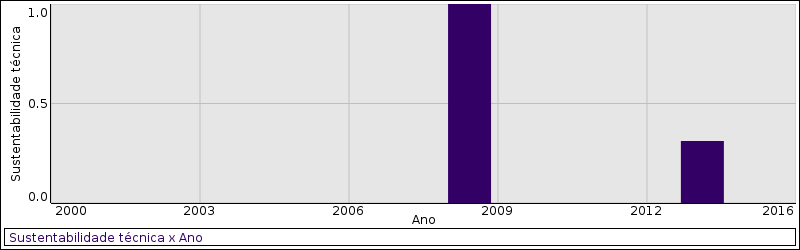
\includegraphics[scale=0.50]{imagens/softwares-charts/jtop.png}
  \caption{Sustentabilidade técnica do Jtop}
\end{figure}


\section{Bogor/Kiasan}
\checkmark download
\checkmark código fonte
\checkmark licença


\begin{table}[H]
\caption{Versões lançadas e número de citações ao Bogor/Kiasan por ano}
\centering
\begin{tabular}{| l | c | c | c | c | c |}
  \hline
  Ano & Versões & Peso da citação & Peso da autoria & Peso final & Sustentabilidade técnica \\
  \hline
            {\bf 2006}
          &
          
          &
          1.00
          &
          0.00
          &
          1.00
          &
            {\color{blue} 1.00}
          \\
            2006
          &
          
          &
          0.50
          &
          0.00
          &
          0.50
          &
          \\
\hline
            2007
          &
          
          &
          0.10
          &
          0.25
          &
          0.12
          &
            {\color{blue} 0.62}
          \\
            2007
          &
          
          &
          0.50
          &
          0.25
          &
          0.62
          &
          \\
            2007
          &
          
          &
          0.50
          &
          0.25
          &
          0.62
          &
          \\
\hline
            2008
          &
          
          &
          0.10
          &
          0.50
          &
          0.15
          &
            {\color{red} 0.15}
          \\
            2008
          &
          
          &
          0.10
          &
          0.50
          &
          0.15
          &
          \\
            2008
          &
          
          &
          0.10
          &
          0.50
          &
          0.15
          &
          \\
\hline
            2009
          &
          
          &
          0.10
          &
          0.25
          &
          0.12
          &
            {\color{blue} 0.62}
          \\
            2009
          &
          
          &
          0.50
          &
          0.25
          &
          0.62
          &
          \\
\hline
            2010
          &
          
          &
          0.10
          &
          0.25
          &
          0.12
          &
            {\color{red} 0.12}
          \\
            2010
          &
          
          &
          0.10
          &
          0.25
          &
          0.12
          &
          \\
            2010
          &
          
          &
          0.10
          &
          0.25
          &
          0.12
          &
          \\
\hline
            2013
          &
          
          &
          0.10
          &
          0.50
          &
          0.15
          &
            {\color{red} 0.15}
          \\
\hline
            2014
          &
          
          &
          0.50
          &
          0.25
          &
          0.62
          &
            {\color{blue} 0.62}
          \\
\hline
            2015
          &
          
          &
          0.10
          &
          0.50
          &
          0.15
          &
            {\color{red} 0.15}
          \\
\hline
\end{tabular}
\end{table}

\begin{figure}[h]
  \center
  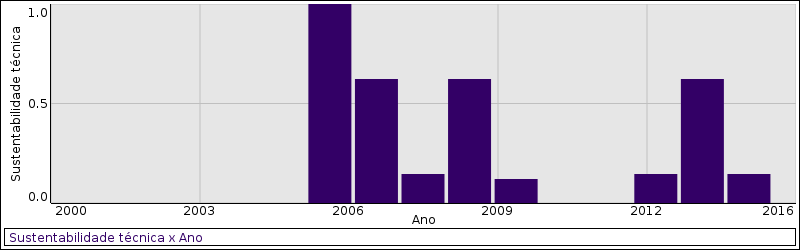
\includegraphics[scale=0.50]{imagens/softwares-charts/kiasan.png}
  \caption{Sustentabilidade técnica do Bogor/Kiasan}
\end{figure}


\section{Loopfrog}
\checkmark download


\begin{table}[H]
\caption{Versões lançadas e número de citações ao Loopfrog por ano}
\centering
\begin{tabular}{| l | c | c | c | c | c |}
  \hline
  Ano & Versões & Peso da citação & Peso da autoria & Peso final & Sustentabilidade técnica \\
  \hline
            {\bf 2009}
          &
          
          &
          1.00
          &
          0.00
          &
          1.00
          &
            {\color{blue} 1.00}
          \\
\hline
            2012
          &
          
          &
          0.10
          &
          0.50
          &
          0.15
          &
            {\color{red} 0.15}
          \\
\hline
            2013
          &
          
          &
          0.10
          &
          0.50
          &
          0.15
          &
            {\color{red} 0.38}
          \\
            2013
          &
          
          &
          0.25
          &
          0.50
          &
          0.38
          &
          \\
            2013
          &
          
          &
          0.25
          &
          0.50
          &
          0.38
          &
          \\
\hline
\end{tabular}
\end{table}

\begin{figure}[h]
  \center
  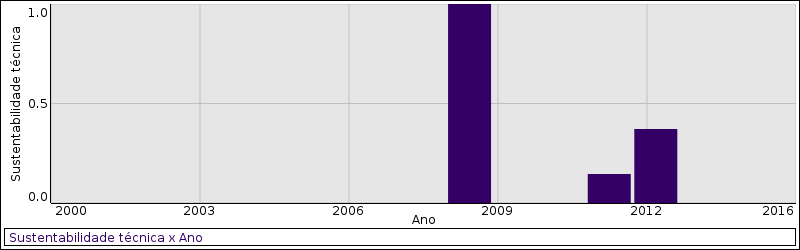
\includegraphics[scale=0.50]{imagens/softwares-charts/loopfrog.png}
  \caption{Sustentabilidade técnica do Loopfrog}
\end{figure}


\section{Lotrack}
\checkmark download
\checkmark código fonte


\begin{table}[H]
\caption{Versões lançadas e número de citações ao Lotrack por ano}
\centering
\begin{tabular}{| l | c | c | c | c | c |}
  \hline
  Ano & Versões & Peso da citação & Peso da autoria & Peso final & Sustentabilidade técnica \\
  \hline
            {\bf 2014}
          &
          
          &
          1.00
          &
          0.00
          &
          1.00
          &
            {\color{blue} 1.00}
          \\
\hline
            2015
          &
          
          &
          0.10
          &
          0.50
          &
          0.15
          &
            {\color{red} 0.15}
          \\
\hline
\end{tabular}
\end{table}

\begin{figure}[h]
  \center
  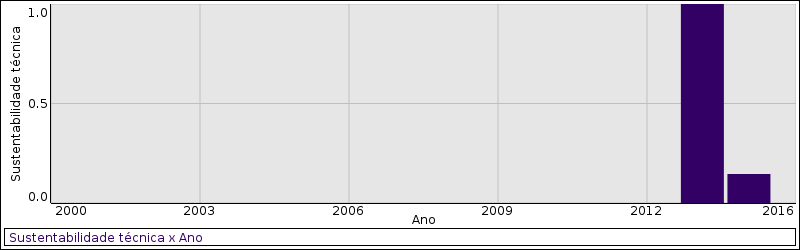
\includegraphics[scale=0.50]{imagens/softwares-charts/lotrack.png}
  \caption{Sustentabilidade técnica do Lotrack}
\end{figure}


\section{MPAnalyzer}
\checkmark download
\checkmark código fonte


\begin{table}[H]
\caption{Versões lançadas e número de citações ao MPAnalyzer por ano}
\centering
\begin{tabular}{| l | c | c | c | c | c |}
  \hline
  Ano & Versões & Peso da citação & Peso da autoria & Peso final & Sustentabilidade técnica \\
  \hline
            {\bf 2014}
          &
          
          &
          1.00
          &
          0.00
          &
          1.00
          &
            {\color{blue} 1.00}
          \\
\hline
\end{tabular}
\end{table}

\begin{figure}[h]
  \center
  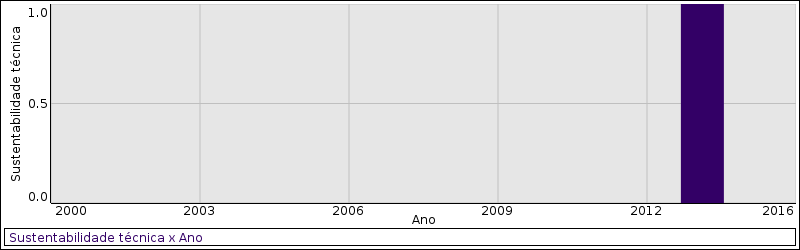
\includegraphics[scale=0.50]{imagens/softwares-charts/mpanalyzer.png}
  \caption{Sustentabilidade técnica do MPAnalyzer}
\end{figure}


\section{MSP}


\begin{table}[H]
\caption{Versões lançadas e número de citações ao MSP por ano}
\centering
\begin{tabular}{| l | c | c | c | c | c |}
  \hline
  Ano & Versões & Peso da citação & Peso da autoria & Peso final & Sustentabilidade técnica \\
  \hline
            2009
          &
          
          &
          0.10
            {\tiny MSP-GCC}
          &
          0.00
          &
          0.10
          &
            {\color{red} 0.10}
          \\
\hline
            {\bf 2010}
          &
          
          &
          1.00
          &
          0.50
          &
          1.00
          &
            {\color{blue} 1.00}
          \\
\hline
\end{tabular}
\end{table}

\begin{figure}[h]
  \center
  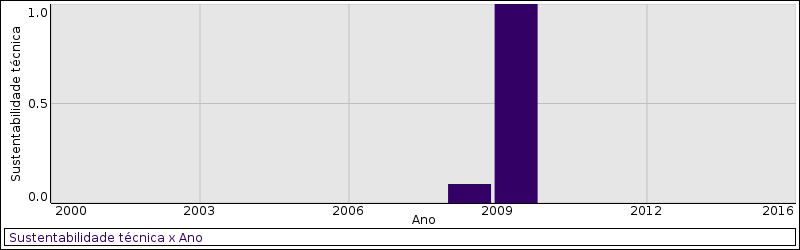
\includegraphics[scale=0.50]{imagens/softwares-charts/msp.png}
  \caption{Sustentabilidade técnica do MSP}
\end{figure}


\section{mygcc}
\checkmark download
\checkmark código fonte
\checkmark licença


\begin{table}[H]
\caption{Versões lançadas e número de citações ao mygcc por ano}
\centering
\begin{tabular}{| l | c | c | c | c | c |}
  \hline
  Ano & Versões & Peso da citação & Peso da autoria & Peso final & Sustentabilidade técnica \\
  \hline
            {\bf 2006}
          &
          
          &
          1.00
          &
          0.00
          &
          1.00
          &
            {\color{blue} 1.00}
          \\
            2006
          &
          
          &
          1.00
          &
          0.00
          &
          1.00
          &
          \\
\hline
            2008
          &
          
          &
          0.50
          &
          0.00
          &
          0.50
          &
            {\color{blue} 0.50}
          \\
\hline
            2009
          &
          
          &
          0.10
          &
          0.50
          &
          0.15
          &
            {\color{red} 0.15}
          \\
            2009
          &
          
          &
          0.10
          &
          0.50
          &
          0.15
          &
          \\
\hline
            2010
          &
          
          &
          0.25
          &
          0.50
          &
          0.38
          &
            {\color{red} 0.38}
          \\
\hline
            2014
          &
          
          &
          0.10
          &
          0.50
          &
          0.15
          &
            {\color{red} 0.15}
          \\
\hline
\end{tabular}
\end{table}

\begin{figure}[h]
  \center
  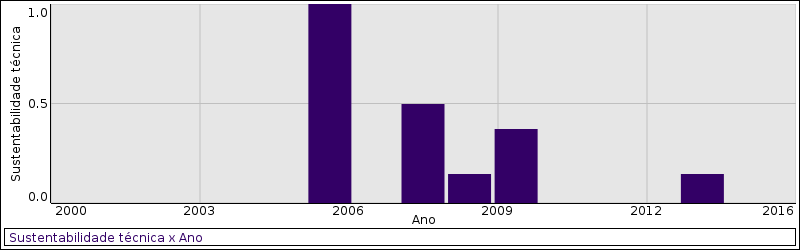
\includegraphics[scale=0.50]{imagens/softwares-charts/mygcc.png}
  \caption{Sustentabilidade técnica do mygcc}
\end{figure}


\section{PARSEWeb}


\begin{table}[H]
\caption{Versões lançadas e número de citações ao PARSEWeb por ano}
\centering
\begin{tabular}{| l | c | c | c | c | c |}
  \hline
  Ano & Versões & Peso da citação & Peso da autoria & Peso final & Sustentabilidade técnica \\
  \hline
            {\bf 2007}
          &
          
          &
          1.00
          &
          0.00
          &
          1.00
          &
            {\color{blue} 1.00}
          \\
\hline
            2008
          &
          
          &
          0.25
          &
          0.50
          &
          0.38
          &
            {\color{red} 0.38}
          \\
            2008
          &
          
          &
          0.10
          &
          0.00
          &
          0.10
          &
          \\
            2008
          &
          
          &
          0.10
          &
          0.50
          &
          0.15
          &
          \\
\hline
            2010
          &
          
          &
          0.10
          &
          0.50
          &
          0.15
          &
            {\color{red} 0.15}
          \\
\hline
            2011
          &
          
          &
          0.10
          &
          0.50
          &
          0.15
          &
            {\color{red} 0.15}
          \\
            2011
          &
          
          &
          0.10
          &
          0.50
          &
          0.15
          &
          \\
            2011
          &
          
          &
          0.10
          &
          0.50
          &
          0.15
          &
          \\
            2011
          &
          
          &
          0.10
          &
          0.50
          &
          0.15
          &
          \\
            2011
          &
          
          &
          0.10
          &
          0.50
          &
          0.15
          &
          \\
\hline
            2012
          &
          
          &
          0.10
          &
          0.50
          &
          0.15
          &
            {\color{red} 0.15}
          \\
            2012
          &
          
          &
          0.10
          &
          0.25
          &
          0.12
          &
          \\
            2012
          &
          
          &
          0.10
          &
          0.25
          &
          0.12
          &
          \\
            2012
          &
          
          &
          0.10
          &
          0.50
          &
          0.15
          &
          \\
            2012
          &
          
          &
          0.10
          &
          0.50
          &
          0.15
          &
          \\
            2012
          &
          
          &
          0.10
          &
          0.50
          &
          0.15
          &
          \\
\hline
            2013
          &
          
          &
          0.10
          &
          0.50
          &
          0.15
          &
            {\color{red} 0.15}
          \\
            2013
          &
          
          &
          0.10
          &
          0.50
          &
          0.15
          &
          \\
            2013
          &
          
          &
          0.10
          &
          0.50
          &
          0.15
          &
          \\
\hline
            2015
          &
          
          &
          0.10
          &
          0.25
          &
          0.12
          &
            {\color{red} 0.12}
          \\
            2015
          &
          
          &
          0.10
          &
          0.10
          &
          0.11
          &
          \\
\hline
            2016
          &
          
          &
          0.10
          &
          0.50
          &
          0.15
          &
            {\color{red} 0.15}
          \\
            2016
          &
          
          &
          0.10
          &
          0.50
          &
          0.15
          &
          \\
            2016
          &
          
          &
          0.10
          &
          0.25
          &
          0.12
          &
          \\
\hline
\end{tabular}
\end{table}

\begin{figure}[h]
  \center
  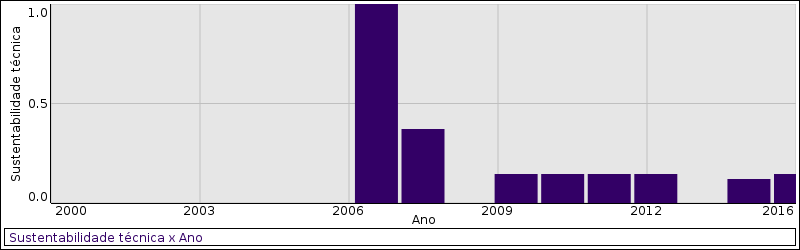
\includegraphics[scale=0.50]{imagens/softwares-charts/parseweb.png}
  \caption{Sustentabilidade técnica do PARSEWeb}
\end{figure}


\section{PAT - Puzzle-Based Automatic Testing}


\begin{table}[H]
\caption{Versões lançadas e número de citações ao PAT por ano}
\centering
\begin{tabular}{| l | c | c | c | c | c |}
  \hline
  Ano & Versões & Peso da citação & Peso da autoria & Peso final & Sustentabilidade técnica \\
  \hline
            {\bf 2012}
          &
          
          &
          1.00
          &
          0.00
          &
          1.00
          &
            {\color{blue} 1.00}
          \\
\hline
            2016
          &
          
          &
          0.10
          &
          0.50
          &
          0.15
          &
            {\color{red} 0.15}
          \\
\hline
\end{tabular}
\end{table}

\begin{figure}[h]
  \center
  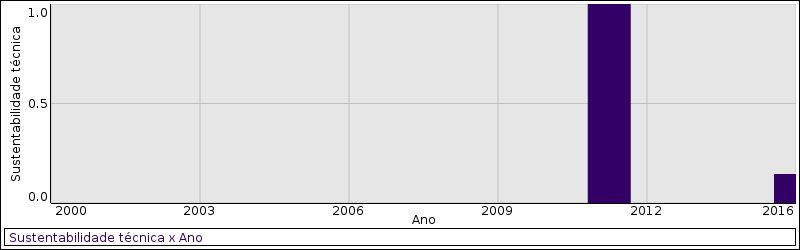
\includegraphics[scale=0.50]{imagens/softwares-charts/pat.png}
  \caption{Sustentabilidade técnica do PAT}
\end{figure}


\section{PHP AiR}
\checkmark download
\checkmark código fonte


\begin{table}[H]
\caption{Versões lançadas e número de citações ao PHP AiR por ano}
\centering
\begin{tabular}{| l | c | c | c | c | c |}
  \hline
  Ano & Versões & Peso da citação & Peso da autoria & Peso final & Sustentabilidade técnica \\
  \hline
        2011 & 1 & - & - & -
        &
          {\color{blue} 1.00}
        \\
\hline
        2012 & 1 & - & - & -
        &
          {\color{blue} 1.00}
        \\
\hline
            2014
          &
          2
          &
          0.10
          &
          0.00
          &
          0.10
          &
            {\color{blue} 1.00}
          \\
            {\bf 2014}
          &
          
          &
          1.00
          &
          0.00
          &
          1.00
          &
          \\
\hline
            2015
          &
          
          &
          0.25
          &
          0.25
          &
          0.31
          &
            {\color{blue} 0.62}
          \\
            2015
          &
          
          &
          0.50
          &
          0.00
          &
          0.50
          &
          \\
            2015
          &
          
          &
          0.25
          &
          0.25
          &
          0.31
          &
          \\
            2015
          &
          
          &
          0.50
          &
          0.25
          &
          0.62
          &
          \\
            2015
          &
          
          &
          0.25
          &
          0.25
          &
          0.31
          &
          \\
\hline
            2016
          &
          
          &
          0.25
          &
          0.10
          &
          0.28
          &
            {\color{red} 0.28}
          \\
\hline
            2017
          &
          
          &
          0.25
          &
          0.25
          &
          0.31
          &
            {\color{red} 0.31}
          \\
\hline
\end{tabular}
\end{table}

\begin{figure}[h]
  \center
  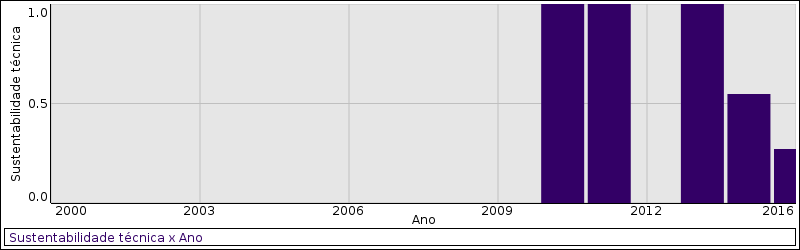
\includegraphics[scale=0.50]{imagens/softwares-charts/php-air.png}
  \caption{Sustentabilidade técnica do PHP AiR}
\end{figure}


\section{protopurity}
\checkmark download
\checkmark código fonte


\begin{table}[H]
\caption{Versões lançadas e número de citações ao protopurity por ano}
\centering
\begin{tabular}{| l | c | c | c | c | c |}
  \hline
  Ano & Versões & Peso da citação & Peso da autoria & Peso final & Sustentabilidade técnica \\
  \hline
            {\bf 2015}
          &
          
          &
          1.00
          &
          0.00
          &
          1.00
          &
            {\color{blue} 1.00}
          \\
\hline
\end{tabular}
\end{table}

\begin{figure}[h]
  \center
  \includegraphics[scale=0.50]{imagens/softwares-charts/protopurity.png}
  \caption{Sustentabilidade técnica do protopurity}
\end{figure}


\section{Pseudogen}
\checkmark download
\checkmark código fonte


\begin{table}[H]
\caption{Versões lançadas e número de citações ao Pseudogen por ano}
\centering
\begin{tabular}{| l | c | c | c | c | c |}
  \hline
  Ano & Versões & Peso da citação & Peso da autoria & Peso final & Sustentabilidade técnica \\
  \hline
            {\bf 2015}
          &
          
          &
          1.00
          &
          0.00
          &
          1.00
          &
            {\color{blue} 1.00}
          \\
\hline
\end{tabular}
\end{table}

\begin{figure}[h]
  \center
  \includegraphics[scale=0.50]{imagens/softwares-charts/pseudogen.png}
  \caption{Sustentabilidade técnica do Pseudogen}
\end{figure}


\section{PtYasm}
\checkmark download
\checkmark código fonte


\begin{table}[H]
\caption{Versões lançadas e número de citações ao PtYasm por ano}
\centering
\begin{tabular}{| l | c | c | c | c | c |}
  \hline
  Ano & Versões & Peso da citação & Peso da autoria & Peso final & Sustentabilidade técnica \\
  \hline
            {\bf 2008}
          &
          
          &
          0.50
          &
          0.00
          &
          0.50
          &
            {\color{blue} 0.50}
          \\
            {\bf 2008}
          &
          
          &
          0.50
          &
          0.00
          &
          0.50
          &
          \\
\hline
\end{tabular}
\end{table}

\begin{figure}[h]
  \center
  \includegraphics[scale=0.50]{imagens/softwares-charts/ptyasm.png}
  \caption{Sustentabilidade técnica do PtYasm}
\end{figure}


\section{PuMoC}


\begin{table}[H]
\caption{Versões lançadas e número de citações ao PuMoC por ano}
\centering
\begin{tabular}{| l | c | c | c | c | c |}
  \hline
  Ano & Versões & Peso da citação & Peso da autoria & Peso final & Sustentabilidade técnica \\
  \hline
            {\bf 2012}
          &
          
          &
          1.00
          &
          0.00
          &
          1.00
          &
            {\color{blue} 1.00}
          \\
\hline
            2013
          &
          
          &
          0.10
          &
          0.10
          &
          0.11
          &
            {\color{red} 0.11}
          \\
\hline
\end{tabular}
\end{table}

\begin{figure}[h]
  \center
  \includegraphics[scale=0.50]{imagens/softwares-charts/pumoc.png}
  \caption{Sustentabilidade técnica do PuMoC}
\end{figure}


\section{PYTHIA}


\begin{table}[H]
\caption{Versões lançadas e número de citações ao PYTHIA por ano}
\centering
\begin{tabular}{| l | c | c | c | c | c |}
  \hline
  Ano & Versões & Peso da citação & Peso da autoria & Peso final & Sustentabilidade técnica \\
  \hline
            {\bf 2013}
          &
          
          &
          1.00
          &
          0.00
          &
          1.00
          &
            {\color{blue} 1.00}
          \\
\hline
            2014
          &
          
          &
          0.50
          &
          0.10
          &
          0.55
          &
            {\color{blue} 0.55}
          \\
\hline
\end{tabular}
\end{table}

\begin{figure}[h]
  \center
  \includegraphics[scale=0.50]{imagens/softwares-charts/pythia.png}
  \caption{Sustentabilidade técnica do PYTHIA}
\end{figure}


\section{ReAssert}
\checkmark download
\checkmark código fonte
\checkmark licença


\begin{table}[H]
\caption{Versões lançadas e número de citações ao ReAssert por ano}
\centering
\begin{tabular}{| l | c | c | c | c | c |}
  \hline
  Ano & Versões & Peso da citação & Peso da autoria & Peso final & Sustentabilidade técnica \\
  \hline
            {\bf 2009}
          &
          2
          &
          1.00
          &
          0.00
          &
          1.00
          &
            {\color{blue} 1.00}
          \\
\hline
            2010
          &
          3
          &
          0.25
          &
          0.25
          &
          0.31
          &
            {\color{blue} 1.00}
          \\
\hline
            2011
          &
          
          &
          0.10
          &
          0.00
          &
          0.10
          &
            {\color{red} 0.25}
          \\
            2011
          &
          
          &
          0.25
          &
          0.00
          &
          0.25
          &
          \\
            2011
          &
          
          &
          0.10
          &
          0.00
          &
          0.10
          &
          \\
            2011
          &
          
          &
          0.10
          &
          0.00
          &
          0.10
          &
          \\
\hline
            2012
          &
          
          &
          0.25
          &
          0.25
          &
          0.31
          &
            {\color{red} 0.31}
          \\
            2012
          &
          
          &
          0.10
          &
          0.25
          &
          0.12
          &
          \\
            2012
          &
          
          &
          0.10
          &
          0.25
          &
          0.12
          &
          \\
\hline
            2013
          &
          
          &
          0.10
          &
          0.50
          &
          0.15
          &
            {\color{red} 0.15}
          \\
            2013
          &
          
          &
          0.10
          &
          0.50
          &
          0.15
          &
          \\
\hline
            2016
          &
          
          &
          0.10
          &
          0.25
          &
          0.12
          &
            {\color{red} 0.12}
          \\
            2016
          &
          
          &
          0.10
            {\tiny COOPE}
          &
          0.25
          &
          0.12
          &
          \\
\hline
\end{tabular}
\end{table}

\begin{figure}[h]
  \center
  \includegraphics[scale=0.50]{imagens/softwares-charts/reassert.png}
  \caption{Sustentabilidade técnica do ReAssert}
\end{figure}


\section{Rêve}


\begin{table}[H]
\caption{Versões lançadas e número de citações ao Rêve por ano}
\centering
\begin{tabular}{| l | c | c | c | c | c |}
  \hline
  Ano & Versões & Peso da citação & Peso da autoria & Peso final & Sustentabilidade técnica \\
  \hline
            {\bf 2014}
          &
          
          &
          1.00
          &
          0.00
          &
          1.00
          &
            {\color{blue} 1.00}
          \\
\hline
\end{tabular}
\end{table}

\begin{figure}[h]
  \center
  \includegraphics[scale=0.50]{imagens/softwares-charts/reve.png}
  \caption{Sustentabilidade técnica do Rêve}
\end{figure}


\section{RRFinder}


\begin{table}[H]
\caption{Versões lançadas e número de citações ao RRFinder por ano}
\centering
\begin{tabular}{| l | c | c | c | c | c |}
  \hline
  Ano & Versões & Peso da citação & Peso da autoria & Peso final & Sustentabilidade técnica \\
  \hline
            {\bf 2011}
          &
          
          &
          1.00
          &
          0.00
          &
          1.00
          &
            {\color{blue} 1.00}
          \\
\hline
            2014
          &
          
          &
          0.10
          &
          0.50
          &
          0.15
          &
            {\color{red} 0.15}
          \\
\hline
            2015
          &
          
          &
          0.10
          &
          0.50
          &
          0.15
          &
            {\color{red} 0.15}
          \\
\hline
\end{tabular}
\end{table}

\begin{figure}[h]
  \center
  \includegraphics[scale=0.50]{imagens/softwares-charts/rrfinder.png}
  \caption{Sustentabilidade técnica do RRFinder}
\end{figure}


\section{Sapid/XML}


\begin{table}[H]
\caption{Versões lançadas e número de citações ao Sapid/XML por ano}
\centering
\begin{tabular}{| l | c | c | c | c | c |}
  \hline
  Ano & Versões & Peso da citação & Peso da autoria & Peso final & Sustentabilidade técnica \\
  \hline
            {\bf 2004}
          &
          
          &
          1.00
          &
          0.00
          &
          1.00
          &
            {\color{blue} 1.00}
          \\
\hline
            2005
          &
          
          &
          0.25
          &
          0.00
          &
          0.25
          &
            {\color{blue} 0.55}
          \\
            2005
          &
          
          &
          0.50
          &
          0.10
          &
          0.55
          &
          \\
\hline
            2006
          &
          
          &
          0.25
          &
          0.10
          &
          0.28
          &
            {\color{red} 0.28}
          \\
\hline
            2012
          &
          
          &
          0.10
          &
          0.50
          &
          0.15
          &
            {\color{red} 0.15}
          \\
\hline
\end{tabular}
\end{table}

\begin{figure}[h]
  \center
  \includegraphics[scale=0.50]{imagens/softwares-charts/sapid-xml.png}
  \caption{Sustentabilidade técnica do Sapid/XML}
\end{figure}


\section{Sonar Qube Plug-in}
\checkmark download
\checkmark código fonte
\checkmark licença


\begin{table}[H]
\caption{Versões lançadas e número de citações ao Sonar Qube Plug-in por ano}
\centering
\begin{tabular}{| l | c | c | c | c | c |}
  \hline
  Ano & Versões & Peso da citação & Peso da autoria & Peso final & Sustentabilidade técnica \\
  \hline
            {\bf 2014}
          &
          
          &
          1.00
          &
          0.00
          &
          1.00
          &
            {\color{blue} 1.00}
          \\
\hline
        2015 & 3 & - & - & -
        &
          {\color{blue} 1.00}
        \\
\hline
        2016 & 1 & - & - & -
        &
          {\color{blue} 1.00}
        \\
\hline
\end{tabular}
\end{table}

\begin{figure}[h]
  \center
  \includegraphics[scale=0.50]{imagens/softwares-charts/sonarqube-plugin.png}
  \caption{Sustentabilidade técnica do Sonar Qube Plug-in}
\end{figure}


\section{SPARTA - Static Program Analysis for Reliable Trusted Apps}
\checkmark download
\checkmark código fonte


\begin{table}[H]
\caption{Versões lançadas e número de citações ao SPARTA por ano}
\centering
\begin{tabular}{| l | c | c | c | c | c |}
  \hline
  Ano & Versões & Peso da citação & Peso da autoria & Peso final & Sustentabilidade técnica \\
  \hline
            2002
          &
          
          &
          0.25
          &
          0.00
          &
          0.25
          &
            {\color{red} 0.25}
          \\
\hline
        2012 & 1 & - & - & -
        &
          {\color{blue} 1.00}
        \\
\hline
        2013 & 7 & - & - & -
        &
          {\color{blue} 1.00}
        \\
\hline
        2014 & 4 & - & - & -
        &
          {\color{blue} 1.00}
        \\
\hline
            {\bf 2015}
          &
          1
          &
          1.00
          &
          0.50
          &
          1.00
          &
            {\color{blue} 1.00}
          \\
\hline
        2016 & 1 & - & - & -
        &
          {\color{blue} 1.00}
        \\
\hline
            2017
          &
          
          &
          0.25
          &
          0.50
          &
          0.38
          &
            {\color{red} 0.38}
          \\
            2017
          &
          
          &
          0.10
          &
          0.50
          &
          0.15
          &
          \\
\hline
\end{tabular}
\end{table}

\begin{figure}[h]
  \center
  \includegraphics[scale=0.50]{imagens/softwares-charts/sparta.png}
  \caption{Sustentabilidade técnica do SPARTA}
\end{figure}


\section{srcML}
\checkmark download
\checkmark código fonte
\checkmark licença


\begin{table}[H]
\caption{Versões lançadas e número de citações ao srcML por ano}
\centering
\begin{tabular}{| l | c | c | c | c | c |}
  \hline
  Ano & Versões & Peso da citação & Peso da autoria & Peso final & Sustentabilidade técnica \\
  \hline
            2002
          &
          
          &
          0.10
          &
          0.00
          &
          0.10
          &
            {\color{red} 0.10}
          \\
\hline
            2003
          &
          
          &
          0.10
          &
          0.50
          &
          0.15
          &
            {\color{red} 0.15}
          \\
\hline
            2004
          &
          
          &
          0.25
          &
          0.50
          &
          0.38
          &
            {\color{red} 0.38}
          \\
            2004
          &
          
          &
          0.25
          &
          0.50
          &
          0.38
          &
          \\
            2004
          &
          
          &
          0.10
          &
          0.50
          &
          0.15
          &
          \\
\hline
            2005
          &
          
          &
          0.25
          &
          0.50
          &
          0.38
          &
            {\color{red} 0.38}
          \\
            2005
          &
          
          &
          0.10
          &
          0.50
          &
          0.15
          &
          \\
            2005
          &
          
          &
          0.10
          &
          0.25
          &
          0.12
          &
          \\
\hline
            2007
          &
          
          &
          0.10
          &
          0.25
          &
          0.12
          &
            {\color{red} 0.12}
          \\
\hline
            2008
          &
          
          &
          0.10
          &
          0.25
          &
          0.12
          &
            {\color{red} 0.12}
          \\
\hline
            2009
          &
          
          &
          0.25
          &
          0.50
          &
          0.38
          &
            {\color{red} 0.38}
          \\
            2009
          &
          
          &
          0.10
          &
          0.50
          &
          0.15
          &
          \\
            2009
          &
          
          &
          0.10
          &
          0.50
          &
          0.15
          &
          \\
\hline
            2010
          &
          
          &
          0.25
          &
          0.25
          &
          0.31
          &
            {\color{red} 0.31}
          \\
\hline
            2011
          &
          3
          &
          0.25
          &
          0.25
          &
          0.31
          &
            {\color{blue} 1.00}
          \\
            2011
          &
          
          &
          0.25
          &
          0.50
          &
          0.38
          &
          \\
            {\bf 2011}
          &
          
          &
          1.00
          &
          0.25
          &
          1.00
          &
          \\
\hline
            2012
          &
          5
          &
          0.25
          &
          0.25
          &
          0.31
          &
            {\color{blue} 1.00}
          \\
            2012
          &
          
          &
          0.25
          &
          0.25
          &
          0.31
          &
          \\
            2012
          &
          
          &
          0.25
          &
          0.25
          &
          0.31
          &
          \\
\hline
            2013
          &
          1
          &
          0.25
          &
          0.25
          &
          0.31
          &
            {\color{blue} 1.00}
          \\
            2013
          &
          
          &
          0.25
          &
          0.50
          &
          0.38
          &
          \\
            2013
          &
          
          &
          0.10
          &
          0.25
          &
          0.12
          &
          \\
            2013
          &
          
          &
          0.10
          &
          0.25
          &
          0.12
          &
          \\
\hline
            2014
          &
          4
          &
          0.25
          &
          0.50
          &
          0.38
          &
            {\color{blue} 1.00}
          \\
            2014
          &
          
          &
          0.25
          &
          0.25
          &
          0.31
          &
          \\
            2014
          &
          
          &
          0.25
          &
          0.50
          &
          0.38
          &
          \\
            2014
          &
          
          &
          0.25
          &
          0.50
          &
          0.38
          &
          \\
\hline
            2015
          &
          1
          &
          0.10
          &
          0.25
          &
          0.12
          &
            {\color{blue} 1.00}
          \\
            2015
          &
          
          &
          0.10
          &
          0.25
          &
          0.12
          &
          \\
            2015
          &
          
          &
          0.25
          &
          0.25
          &
          0.31
          &
          \\
\hline
            2016
          &
          
          &
          0.25
          &
          0.25
          &
          0.31
          &
            {\color{blue} 0.62}
          \\
            2016
          &
          
          &
          0.50
          &
          0.25
          &
          0.62
          &
          \\
            2016
          &
          
          &
          0.25
          &
          0.25
          &
          0.31
          &
          \\
            2016
          &
          
          &
          0.25
          &
          0.25
          &
          0.31
          &
          \\
            2016
          &
          
          &
          0.25
          &
          0.25
          &
          0.31
          &
          \\
            2016
          &
          
          &
          0.50
          &
          0.25
          &
          0.62
          &
          \\
\hline
            2017
          &
          
          &
          0.25
          &
          0.25
          &
          0.31
          &
            {\color{red} 0.38}
          \\
            2017
          &
          
          &
          0.25
          &
          0.50
          &
          0.38
          &
          \\
            2017
          &
          
          &
          0.10
            {\tiny srcQL}
          &
          0.25
          &
          0.12
          &
          \\
\hline
\end{tabular}
\end{table}

\begin{figure}[h]
  \center
  \includegraphics[scale=0.50]{imagens/softwares-charts/srcml.png}
  \caption{Sustentabilidade técnica do srcML}
\end{figure}


\section{SWAT - Search based Web Application Tester}


\begin{table}[H]
\caption{Versões lançadas e número de citações ao SWAT por ano}
\centering
\begin{tabular}{| l | c | c | c | c | c |}
  \hline
  Ano & Versões & Peso da citação & Peso da autoria & Peso final & Sustentabilidade técnica \\
  \hline
            {\bf 2011}
          &
          
          &
          1.00
          &
          0.00
          &
          1.00
          &
            {\color{blue} 1.00}
          \\
\hline
            2012
          &
          
          &
          0.25
          &
          0.10
          &
          0.28
          &
            {\color{red} 0.28}
          \\
\hline
            2013
          &
          
          &
          0.10
          &
          0.50
          &
          0.15
          &
            {\color{red} 0.15}
          \\
\hline
            2014
          &
          
          &
          0.25
          &
          0.10
          &
          0.28
          &
            {\color{red} 0.28}
          \\
\hline
\end{tabular}
\end{table}

\begin{figure}[h]
  \center
  \includegraphics[scale=0.50]{imagens/softwares-charts/swat.png}
  \caption{Sustentabilidade técnica do SWAT}
\end{figure}


\section{TACLE - Type Analysis and CalL graph construction for Eclipse}
\checkmark download
\checkmark código fonte


\begin{table}[H]
\caption{Versões lançadas e número de citações ao TACLE por ano}
\centering
\begin{tabular}{| l | c | c | c | c | c |}
  \hline
  Ano & Versões & Peso da citação & Peso da autoria & Peso final & Sustentabilidade técnica \\
  \hline
            2005
          &
          
          &
          0.25
          &
          0.00
          &
          0.25
          &
            {\color{red} 0.25}
          \\
\hline
            {\bf 2006}
          &
          
          &
          1.00
          &
          0.10
          &
          1.00
          &
            {\color{blue} 1.00}
          \\
            2006
          &
          
          &
          0.10
          &
          0.10
          &
          0.11
          &
          \\
\hline
\end{tabular}
\end{table}

\begin{figure}[h]
  \center
  \includegraphics[scale=0.50]{imagens/softwares-charts/tacle.png}
  \caption{Sustentabilidade técnica do TACLE}
\end{figure}


\section{TEBA}
\checkmark download
\checkmark código fonte


\begin{table}[H]
\caption{Versões lançadas e número de citações ao TEBA por ano}
\centering
\begin{tabular}{| l | c | c | c | c | c |}
  \hline
  Ano & Versões & Peso da citação & Peso da autoria & Peso final & Sustentabilidade técnica \\
  \hline
        2010 & 1 & - & - & -
        &
          {\color{blue} 1.00}
        \\
\hline
        2011 & 5 & - & - & -
        &
          {\color{blue} 1.00}
        \\
\hline
        2012 & 4 & - & - & -
        &
          {\color{blue} 1.00}
        \\
\hline
        2013 & 5 & - & - & -
        &
          {\color{blue} 1.00}
        \\
\hline
            {\bf 2014}
          &
          5
          &
          1.00
          &
          0.00
          &
          1.00
          &
            {\color{blue} 1.00}
          \\
\hline
        2016 & 1 & - & - & -
        &
          {\color{blue} 1.00}
        \\
\hline
\end{tabular}
\end{table}

\begin{figure}[h]
  \center
  \includegraphics[scale=0.50]{imagens/softwares-charts/teba.png}
  \caption{Sustentabilidade técnica do TEBA}
\end{figure}


\section{TestEra}


\begin{table}[H]
\caption{Versões lançadas e número de citações ao TestEra por ano}
\centering
\begin{tabular}{| l | c | c | c | c | c |}
  \hline
  Ano & Versões & Peso da citação & Peso da autoria & Peso final & Sustentabilidade técnica \\
  \hline
            {\bf 2001}
          &
          
          &
          1.00
          &
          0.00
          &
          1.00
          &
            {\color{blue} 1.00}
          \\
\hline
            2002
          &
          
          &
          0.10
          &
          0.00
          &
          0.10
          &
            {\color{red} 0.10}
          \\
\hline
            2004
          &
          
          &
          0.10
          &
          0.25
          &
          0.12
          &
            {\color{red} 0.12}
          \\
\hline
            2005
          &
          
          &
          0.10
          &
          0.25
          &
          0.12
          &
            {\color{red} 0.31}
          \\
            2005
          &
          
          &
          0.25
          &
          0.25
          &
          0.31
          &
          \\
\hline
            2006
          &
          
          &
          0.10
            {\tiny aDeryaft compatible}
          &
          0.25
          &
          0.12
          &
            {\color{red} 0.12}
          \\
\hline
            2007
          &
          
          &
          0.25
          &
          0.25
          &
          0.31
          &
            {\color{red} 0.31}
          \\
            2007
          &
          
          &
          0.25
          &
          0.25
          &
          0.31
          &
          \\
            2007
          &
          
          &
          0.10
          &
          0.25
          &
          0.12
          &
          \\
            2007
          &
          
          &
          0.25
          &
          0.25
          &
          0.31
          &
          \\
\hline
            2008
          &
          
          &
          0.10
          &
          0.25
          &
          0.12
          &
            {\color{red} 0.31}
          \\
            2008
          &
          
          &
          0.25
          &
          0.25
          &
          0.31
          &
          \\
\hline
            2009
          &
          
          &
          0.10
          &
          0.25
          &
          0.12
          &
            {\color{red} 0.12}
          \\
            2009
          &
          
          &
          0.10
          &
          0.25
          &
          0.12
          &
          \\
\hline
            2010
          &
          
          &
          0.10
          &
          0.25
          &
          0.12
          &
            {\color{red} 0.12}
          \\
            2010
          &
          
          &
          0.10
          &
          0.25
          &
          0.12
          &
          \\
\hline
            2011
          &
          
          &
          0.10
          &
          0.10
          &
          0.11
          &
            {\color{red} 0.12}
          \\
            2011
          &
          
          &
          0.10
          &
          0.25
          &
          0.12
          &
          \\
            2011
          &
          
          &
          0.10
          &
          0.25
          &
          0.12
          &
          \\
\hline
            2012
          &
          
          &
          0.10
          &
          0.10
          &
          0.11
          &
            {\color{red} 0.12}
          \\
            2012
          &
          
          &
          0.10
          &
          0.25
          &
          0.12
          &
          \\
\hline
            2013
          &
          
          &
          0.10
          &
          0.50
          &
          0.15
          &
            {\color{red} 0.15}
          \\
\hline
            2014
          &
          
          &
          0.10
          &
          0.50
          &
          0.15
          &
            {\color{red} 0.15}
          \\
\hline
\end{tabular}
\end{table}

\begin{figure}[h]
  \center
  \includegraphics[scale=0.50]{imagens/softwares-charts/testera.png}
  \caption{Sustentabilidade técnica do TestEra}
\end{figure}


\section{Vdiff}


\begin{table}[H]
\caption{Versões lançadas e número de citações ao Vdiff por ano}
\centering
\begin{tabular}{| l | c | c | c | c | c |}
  \hline
  Ano & Versões & Peso da citação & Peso da autoria & Peso final & Sustentabilidade técnica \\
  \hline
            {\bf 2010}
          &
          
          &
          1.00
          &
          0.00
          &
          1.00
          &
            {\color{blue} 1.00}
          \\
\hline
            2011
          &
          
          &
          0.10
          &
          0.50
          &
          0.15
          &
            {\color{red} 0.15}
          \\
            2011
          &
          
          &
          0.10
          &
          0.50
          &
          0.15
          &
          \\
\hline
            2015
          &
          
          &
          0.10
          &
          0.50
          &
          0.15
          &
            {\color{red} 0.15}
          \\
\hline
            2016
          &
          
          &
          0.10
          &
          0.50
          &
          0.15
          &
            {\color{red} 0.15}
          \\
\hline
\end{tabular}
\end{table}

\begin{figure}[h]
  \center
  \includegraphics[scale=0.50]{imagens/softwares-charts/vdiff.png}
  \caption{Sustentabilidade técnica do Vdiff}
\end{figure}


\section{WALA}
\checkmark download
\checkmark código fonte
\checkmark licença


\begin{table}[H]
\caption{Versões lançadas e número de citações ao WALA por ano}
\centering
\begin{tabular}{| l | c | c | c | c | c |}
  \hline
  Ano & Versões & Peso da citação & Peso da autoria & Peso final & Sustentabilidade técnica \\
  \hline
        2006 & 1 & - & - & -
        &
          {\color{blue} 1.00}
        \\
\hline
        2007 & 6 & - & - & -
        &
          {\color{blue} 1.00}
        \\
\hline
            2008
          &
          4
          &
          0.25
          &
          0.00
          &
          0.25
          &
            {\color{blue} 1.00}
          \\
\hline
            2009
          &
          6
          &
          0.25
          &
          0.50
          &
          0.38
          &
            {\color{blue} 1.00}
          \\
\hline
            {\bf 2010}
          &
          4
          &
          1.00
          &
          0.25
          &
          1.00
          &
            {\color{blue} 1.00}
          \\
\hline
            2011
          &
          3
          &
          0.25
          &
          0.50
          &
          0.38
          &
            {\color{blue} 1.00}
          \\
\hline
            2012
          &
          2
          &
          0.25
          &
          0.50
          &
          0.38
          &
            {\color{blue} 1.00}
          \\
            2012
          &
          
          &
          0.10
          &
          0.50
          &
          0.15
          &
          \\
\hline
            2013
          &
          4
          &
          0.10
          &
          0.25
          &
          0.12
          &
            {\color{blue} 1.00}
          \\
\hline
        2015 & 2 & - & - & -
        &
          {\color{blue} 1.00}
        \\
\hline
            2016
          &
          1
          &
          0.10
          &
          0.25
          &
          0.12
          &
            {\color{blue} 1.00}
          \\
            2016
          &
          
          &
          0.25
          &
          0.25
          &
          0.31
          &
          \\
            2016
          &
          
          &
          0.10
          &
          0.25
          &
          0.12
          &
          \\
\hline
            2017
          &
          4
          &
          0.10
          &
          0.50
          &
          0.15
          &
            {\color{blue} 1.00}
          \\
\hline
\end{tabular}
\end{table}

\begin{figure}[h]
  \center
  \includegraphics[scale=0.50]{imagens/softwares-charts/wala.png}
  \caption{Sustentabilidade técnica do WALA}
\end{figure}


\section{Wrangler}
\checkmark download
\checkmark código fonte
\checkmark licença


\begin{table}[H]
\caption{Versões lançadas e número de citações ao Wrangler por ano}
\centering
\begin{tabular}{| l | c | c | c | c | c |}
  \hline
  Ano & Versões & Peso da citação & Peso da autoria & Peso final & Sustentabilidade técnica \\
  \hline
            2006
          &
          
          &
          0.25
          &
          0.00
          &
          0.25
          &
            {\color{red} 0.25}
          \\
\hline
            2008
          &
          
          &
          0.10
          &
          0.00
          &
          0.10
          &
            {\color{red} 0.25}
          \\
            2008
          &
          
          &
          0.25
          &
          0.00
          &
          0.25
          &
          \\
            2008
          &
          
          &
          0.10
          &
          0.00
          &
          0.10
          &
          \\
            2008
          &
          
          &
          0.10
          &
          0.00
          &
          0.10
          &
          \\
\hline
            2009
          &
          
          &
          0.10
          &
          0.25
          &
          0.12
          &
            {\color{blue} 0.62}
          \\
            2009
          &
          
          &
          0.25
          &
          0.25
          &
          0.31
          &
          \\
            2009
          &
          
          &
          0.25
          &
          0.25
          &
          0.31
          &
          \\
            2009
          &
          
          &
          0.50
          &
          0.25
          &
          0.62
          &
          \\
\hline
            2010
          &
          
          &
          0.10
          &
          0.25
          &
          0.12
          &
            {\color{blue} 1.00}
          \\
            2010
          &
          
          &
          0.10
          &
          0.50
          &
          0.15
          &
          \\
            2010
          &
          
          &
          0.10
          &
          0.25
          &
          0.12
          &
          \\
            2010
          &
          
          &
          0.25
          &
          0.25
          &
          0.31
          &
          \\
            {\bf 2010}
          &
          
          &
          1.00
          &
          0.25
          &
          1.00
          &
          \\
\hline
            2011
          &
          
          &
          0.50
          &
          0.10
          &
          0.55
          &
            {\color{blue} 0.55}
          \\
\hline
            2012
          &
          
          &
          0.10
          &
          0.50
          &
          0.15
          &
            {\color{blue} 0.62}
          \\
            2012
          &
          
          &
          0.50
          &
          0.25
          &
          0.62
          &
          \\
            2012
          &
          
          &
          0.50
          &
          0.25
          &
          0.62
          &
          \\
            2012
          &
          
          &
          0.10
          &
          0.25
          &
          0.12
          &
          \\
            2012
          &
          
          &
          0.10
          &
          0.25
          &
          0.12
          &
          \\
\hline
            2013
          &
          1
          &
          0.10
          &
          0.50
          &
          0.15
          &
            {\color{blue} 1.00}
          \\
            2013
          &
          
          &
          0.25
          &
          0.25
          &
          0.31
          &
          \\
            2013
          &
          
          &
          0.25
          &
          0.25
          &
          0.31
          &
          \\
\hline
            2014
          &
          1
          &
          0.50
          &
          0.25
          &
          0.62
          &
            {\color{blue} 1.00}
          \\
            2014
          &
          
          &
          0.50
          &
          0.25
          &
          0.62
          &
          \\
            2014
          &
          
          &
          0.10
          &
          0.25
          &
          0.12
          &
          \\
            2014
          &
          
          &
          0.10
          &
          0.25
          &
          0.12
          &
          \\
\hline
            2015
          &
          1
          &
          0.10
          &
          0.25
          &
          0.12
          &
            {\color{blue} 1.00}
          \\
            2015
          &
          
          &
          0.25
          &
          0.10
          &
          0.28
          &
          \\
\hline
            2016
          &
          
          &
          0.25
          &
          0.50
          &
          0.38
          &
            {\color{red} 0.38}
          \\
            2016
          &
          
          &
          0.25
          &
          0.25
          &
          0.31
          &
          \\
            2016
          &
          
          &
          0.10
          &
          0.50
          &
          0.15
          &
          \\
\hline
            2017
          &
          
          &
          0.10
          &
          0.25
          &
          0.12
          &
            {\color{red} 0.12}
          \\
\hline
\end{tabular}
\end{table}

\begin{figure}[h]
  \center
  \includegraphics[scale=0.50]{imagens/softwares-charts/wrangler.png}
  \caption{Sustentabilidade técnica do Wrangler}
\end{figure}


\section{XOgastan}


\begin{table}[H]
\caption{Versões lançadas e número de citações ao XOgastan por ano}
\centering
\begin{tabular}{| l | c | c | c | c | c |}
  \hline
  Ano & Versões & Peso da citação & Peso da autoria & Peso final & Sustentabilidade técnica \\
  \hline
            {\bf 2003}
          &
          
          &
          1.00
          &
          0.00
          &
          1.00
          &
            {\color{blue} 1.00}
          \\
\hline
            2004
          &
          
          &
          0.10
          &
          0.50
          &
          0.15
          &
            {\color{red} 0.15}
          \\
\hline
            2006
          &
          
          &
          0.10
          &
          0.50
          &
          0.15
          &
            {\color{red} 0.15}
          \\
\hline
            2008
          &
          
          &
          0.10
          &
          0.50
          &
          0.15
          &
            {\color{red} 0.15}
          \\
\hline
            2011
          &
          
          &
          0.10
          &
          0.50
          &
          0.15
          &
            {\color{red} 0.15}
          \\
\hline
\end{tabular}
\end{table}

\begin{figure}[h]
  \center
  \includegraphics[scale=0.50]{imagens/softwares-charts/xogastan.png}
  \caption{Sustentabilidade técnica do XOgastan}
\end{figure}





% **ATENÇÃO** não editar este arquivo!
%
% o conteúdo deste arquivo é gerado pelo script bin/softwares-summary e pelo
% template capitulos/softwares-summary.tex.epl

\xchapter{Dados dos softwares acadêmicos}{Este capítulo apresenta
os dados coletados para cada software acadêmico selecionado na
revisão estruturada}
\label{softwares-summary}

\section{2LS - 2nd order Logic Solving}

Análise de terminação para programas C usando resumo interprocedural baseado em modelos
publicado no ASE 2015,
disponibilizado em \url{http://svn.cprover.org/wiki/doku.php?id=2ls for program analysis},
disponível,
como software livre
sob uma licença BSD.

Software com lançamentos ocasionais,
7 versões lançadas
entre 2015 e 2017,
escrito em C++,
uma busca por citações no {\bf IEEE Xplore} por
\texttt{(('2nd order Logic Solving') AND 2LS)}
e no {\bf ACM} por
\texttt{content.ftsec:(2LS) AND (order) AND (Logic) AND (Solving)}
retornou
37 resultados,
apenas um faz referência ao software.

\begin{itemize}
\item Chen Y. H. and David C. and Kroening D. and Schrammel P. and Wachter B.
      2015.
        \textbf{\textit{ Synthesising Interprocedural Bit-Precise Termination Proofs (T)}}.
      [
          cita
          usa
          contribui
          cria
      ]
são os primeiros autores a publicar sobre o software.
\end{itemize}
\section{AccessAnalysis}

Cálculo de métricas IGAT e IGAM
publicado no SCAM 2012,
disponibilizado em \url{http://accessanalysis.sourceforge.net},
disponível,
como software livre
sob uma licença EPL.

Software considerado obsoleto,
4 versões lançadas
entre 2010 e 2012,
escrito em Java,
uma busca por citações no {\bf IEEE Xplore} por
\texttt{(AccessAnalysis)}
e no {\bf ACM} por
\texttt{content.ftsec:(+AccessAnalysis +Tool +Java +Modifiers)}
retornou
8 resultados,
{\bf 2} fazem referência ao software.

\begin{itemize}
\item Zoller C. and Schmolitzky A.
      2012.
        \textit{ Measuring Inappropriate Generosity with Access Modifiers in Java Systems}.
      [
          cita
      ]
são os primeiros autores a publicar sobre o software.
\item Zoller C. and Schmolitzky A.
      2012.
        \textbf{\textit{ AccessAnalysis: A Tool for Measuring the Appropriateness of Access Modifiers in Java Systems}}.
      [
          cita
          usa
          contribui
          cria
      ]
são os primeiros autores a publicar sobre o software.
\end{itemize}
\section{APIExample}

Extração de informações de API Java e documentação automática com exemplos
publicado no ASE 2011,
disponibilizado em \url{http://www.apiexample.com},
inacessível.

Software sem informações sobre lançamentos ou releases,
uma busca por citações no {\bf IEEE Xplore} por
\texttt{((APIExample) AND Java)}
e no {\bf ACM} por
\texttt{content.ftsec:(+APIExample +Java)}
retornou
16 resultados,
{\bf 4} fazem referência ao software.

\begin{itemize}
\item Wang L. and Fang L. and Wang L. and Li G. and Xie B. and Yang F.
      2011.
        \textbf{\textit{ APIExample: An effective web search based usage example recommendation system for java APIs}}.
      [
          cita
          usa
          contribui
          cria
      ]
são os primeiros autores a publicar sobre o software.
\item Zhu Z. and Zou Y. and Jin Y. and Xie B.
      2013.
        \textit{ Generating API-usage Example for Project Developers}.
      [
          cita
      ]
uma parte dos autores já publicou sobre o software em anos anteriores.
\item Montandon E. J. and Borges H. and Felix D. and Valente T. M.
      2013.
        \textit{ Documenting APIs with examples: Lessons learned with the APIMiner platform}.
      [
          cita
      ]
uma parte dos autores já publicou sobre o software em anos anteriores.
\item Yu H. and Song W. and Mine T.
      2016.
        \textit{ APIBook: An Effective Approach for Finding APIs}.
      [
          cita
      ]
nenhum dos autores publicou sobre o software antes.
\end{itemize}
\section{BEG - Bandera environment generator}

Criação automática de ambientes para verificação de modelos Java
publicado no ASE 2003,
disponibilizado em \url{http://bandera.projects.cs.ksu.edu/},
inacessível.

Software sem informações sobre lançamentos ou releases,
uma busca por citações no {\bf IEEE Xplore} por
\texttt{(("Bandera environment generator") AND BEG)}
e no {\bf ACM} por
\texttt{content.ftsec:(+"Bandera environment generator" +BEG)}
retornou
10 resultados,
{\bf 9} fazem referência ao software.

\begin{itemize}
\item Tkachuk O. and Dwyer B. M. and Pasareanu S. C.
      2003.
        \textbf{\textit{ Automated environment generation for software model checking}}.
      [
          cita
          usa
          contribui
          cria
      ]
são os primeiros autores a publicar sobre o software.
\item Dwyer B. M. and Robby and Tkachuk O. and Visser W.
      2004.
        \textit{ Analyzing interaction orderings with model checking}.
      [
          cita
          usa
      ]
uma parte dos autores já publicou sobre o software em anos anteriores.
\item Tkachuk O. and Rajan P. S.
      2006.
        \textit{ Application of Automated Environment Generation to Commercial Software}.
      [
          cita
          usa
      ]
uma parte dos autores já publicou sobre o software em anos anteriores.
\item Mutilin V.
      2006.
        \textit{ Concurrent Testing of Java Components Using Java PathFinder}.
      [
          cita
      ]
uma parte dos autores já publicou sobre o software em anos anteriores.
\item Tkachuk O. and Rajan P. S.
      2007.
        \textit{ Combining Environment Generation and Slicing for Modular Software Model Checking}.
      [
          cita
          usa
      ]
uma parte dos autores já publicou sobre o software em anos anteriores.
\item Parizek P. and Plasil F.
      2007.
        \textit{ Partial Verification of Software Components: Heuristics for Environment Construction}.
      [
          cita
      ]
nenhum dos autores publicou sobre o software antes.
\item Parizek P. and Plasil F.
      2010.
        \textit{ Assume-guarantee verification of software components in SOFA 2 framework}.
      [
          cita
      ]
todos os autores já publicaram sobre o software em anos anteriores.
\item Tkachuk O. and Dwyer B. M.
      2010.
        \textit{ Environment generation for validating event-driven software using model checking}.
      [
          cita
          usa
          contribui
      ]
todos os autores já publicaram sobre o software em anos anteriores.
\item Siavashi F. and Truscan D.
      2015.
        \textit{ Environment Modeling in Model-based Testing: Concepts, Prospects and Research Challenges: A Systematic Literature Review}.
      [
          cita
      ]
nenhum dos autores publicou sobre o software antes.
\end{itemize}
\section{ccJava - Class-based Crosscutting Language for Java}

Linguagem orientada a aspectos
publicado no ASE 2007,
disponibilizado em \url{http://posl.minnie.ai.kyutech.ac.jp/},
inacessível.

Software sem informações sobre lançamentos ou releases,
uma busca por citações no {\bf IEEE Xplore} por
\texttt{(ccJava)}
e no {\bf ACM} por
\texttt{content.ftsec:(+ccJava)}
retornou
7 resultados,
{\bf 5} fazem referência ao software.

\begin{itemize}
\item Ubayashi N. and Sakai A. and Tamai T.
      2007.
        \textit{ An Interface Mechanism for Encapsulating Weaving in Class-based AOP}.
      [
          cita
      ]
são os primeiros autores a publicar sobre o software.
\item Ubayashi N. and Sakai A. and Tamai T.
      2007.
        \textbf{\textit{ An Aspect-oriented Weaving Mechanism Based on Component and Connector Architecture}}.
      [
          cita
          usa
          contribui
          cria
      ]
são os primeiros autores a publicar sobre o software.
\item Ubayashi N. and Sato Y. and Sakai A. and Tamai T.
      2008.
        \textit{ Alloy-Based Lightweight Verification for Aspect-Oriented Architecture}.
      [
          cita
          usa
          contribui
      ]
são os primeiros autores a publicar sobre o software.
\item Ubayashi N. and Akatoki H. and Nomura J.
      2009.
        \textit{ Pointcut-based Architectural Interface for Bridging a Gap Between Design and Implementation}.
      [
          cita
          usa
          contribui
      ]
uma parte dos autores já publicou sobre o software em anos anteriores.
\item Ubayashi N. and Nomura J. and Tamai T.
      2010.
        \textit{ Archface: a contract place where architectural design and code meet together}.
      [
          cita
      ]
todos os autores já publicaram sobre o software em anos anteriores.
\end{itemize}
\section{CIVL - Concurrency intermediate verification language}

Framework para verificação de programas concorrentes
publicado no ASE 2015,
disponibilizado em \url{http://vsl.cis.udel.edu/civl/},
disponível,
como software livre
sob uma licença GPL.

Software com lançamentos frequentes,
36 versões lançadas
entre 2015 e 2017,
escrito em C,
uma busca por citações no {\bf IEEE Xplore} por
\texttt{(('concurrency intermediate verification') AND CIVL)}
e no {\bf ACM} por
\texttt{content.ftsec:(+civl +concurrency +intermediate +verification +language)}
retornou
8 resultados,
{\bf 6} fazem referência ao software.

\begin{itemize}
\item L\'{o}pez A. H. and Marques B. R. E. and Martins F. and Ng N. and Santos C. and Vasconcelos T. V. and Yoshida N.
      2015.
        \textit{ Protocol-based Verification of Message-passing Parallel Programs}.
      [
          cita
      ]
são os primeiros autores a publicar sobre o software.
\item Siegel F. S. and Zheng M. and Luo Z. and Zirkel K. T. and Marianiello V. A. and Edenhofner G. J. and Dwyer B. M. and Rogers S. M.
      2015.
        \textit{ CIVL: the concurrency intermediate verification language}.
      [
          cita
      ]
são os primeiros autores a publicar sobre o software.
\item Gopalakrishnan G. and Sawaya J.
      2015.
        \textit{ Achieving Formal Parallel Program Debugging by Incentivizing CS/HPC Collaborative Tool Development}.
      [
          cita
      ]
são os primeiros autores a publicar sobre o software.
\item Zheng M. and Rogers S. M. and Luo Z. and Dwyer B. M. and Siegel F. S.
      2015.
        \textbf{\textit{ CIVL: Formal Verification of Parallel Programs}}.
      [
          cita
          usa
          contribui
          cria
      ]
são os primeiros autores a publicar sobre o software.
\item Siegel F. S.
      2017.
        \textit{ CIVL Solutions to Verifythis 2016 Challenges}.
      [
          cita
      ]
uma parte dos autores já publicou sobre o software em anos anteriores.
\item Jasper M. and Fecke M. and Steffen B. and Schordan M. and Meijer J. and Pol de van J. and Howar F. and Siegel F. S.
      2017.
        \textit{ The RERS 2017 Challenge and Workshop (Invited Paper)}.
      [
          cita
      ]
uma parte dos autores já publicou sobre o software em anos anteriores.
\end{itemize}
\section{CodeBoost}

Transformação source-to-source para otimização de programas C++
publicado no SCAM 2003,
disponibilizado em \url{http://codeboost.org},
disponível,
como software livre
sob uma licença GPL v2.

Software com lançamentos ocasionais,
134 versões lançadas
entre 2000 e 2004,
escrito em C,
uma busca por citações no {\bf IEEE Xplore} por
\texttt{((CodeBoost) AND C++)}
e no {\bf ACM} por
\texttt{content.ftsec:(+CodeBoost +"C++" +Tool)}
retornou
25 resultados,
{\bf 15} fazem referência ao software.

\begin{itemize}
\item Bagge S. O. and Kalleberg T. K. and Haveraaen M. and Visser E.
      2003.
        \textbf{\textit{ Design of the CodeBoost transformation system for domain-specific optimisation of C++ programs}}.
      [
          cita
          usa
          contribui
          cria
      ]
são os primeiros autores a publicar sobre o software.
\item L\"{a}mmel R. and Visser E. and Visser J.
      2003.
        \textit{ Strategic Programming Meets Adaptive Programming}.
      [
          cita
      ]
são os primeiros autores a publicar sobre o software.
\item Schordan M. and Quinlan D.
      2005.
        \textit{ Specifying transformation sequences as computation on program fragments with an abstract attribute grammar}.
      [
          cita
      ]
uma parte dos autores já publicou sobre o software em anos anteriores.
\item Visser E.
      2005.
        \textit{ Transformations for abstractions}.
      [
          cita
      ]
uma parte dos autores já publicou sobre o software em anos anteriores.
\item Mernik M. and Heering J. and Sloane M. A.
      2005.
        \textit{ When and How to Develop Domain-specific Languages}.
      [
          cita
      ]
nenhum dos autores publicou sobre o software antes.
\item Bravenboer M. and Kalleberg T. K. and Vermaas R. and Visser E.
      2006.
        \textit{ Stratego/XT 0.16: Components for Transformation Systems}.
      [
          cita
      ]
uma parte dos autores já publicou sobre o software em anos anteriores.
\item Quinlan D. and Schordan M. and Vuduc R. and Yi Q.
      2006.
        \textit{ Annotating user-defined abstractions for optimization}.
      [
          cita
      ]
uma parte dos autores já publicou sobre o software em anos anteriores.
\item Gottschling P. and Lumsdaine A.
      2008.
        \textit{ Integrating Semantics and Compilation: Using C++ Concepts to Develop Robust and Efficient Reusable Libraries}.
      [
          cita
      ]
nenhum dos autores publicou sobre o software antes.
\item Willcock J. J. and Lumsdaine A. and Quinlan J. D.
      2009.
        \textit{ Reusable, Generic Program Analyses and Transformations}.
      [
          cita
      ]
uma parte dos autores já publicou sobre o software em anos anteriores.
\item Tang X. and J\"{a}rvi J.
      2010.
        \textit{ Generic Flow-sensitive Optimizing Transformations in C++ with Concepts}.
      [
          cita
      ]
nenhum dos autores publicou sobre o software antes.
\item Brown J. K. and Sujeeth K. A. and Lee J. H. and Rompf T. and Chafi H. and Odersky M. and Olukotun K.
      2011.
        \textit{ A Heterogeneous Parallel Framework for Domain-Specific Languages}.
      [
          cita
      ]
nenhum dos autores publicou sobre o software antes.
\item Chafi H. and Sujeeth K. A. and Brown J. K. and Lee H. and Atreya R. A. and Olukotun K.
      2011.
        \textit{ A Domain-specific Approach to Heterogeneous Parallelism}.
      [
          cita
      ]
nenhum dos autores publicou sobre o software antes.
\item Hong S. and Chafi H. and Sedlar E. and Olukotun K.
      2012.
        \textit{ Green-Marl: A DSL for Easy and Efficient Graph Analysis}.
      [
          cita
      ]
uma parte dos autores já publicou sobre o software em anos anteriores.
\item Keep W. A. and Dybvig K. R.
      2013.
        \textit{ A Nanopass Framework for Commercial Compiler Development}.
      [
          cita
      ]
nenhum dos autores publicou sobre o software antes.
\item Scherr M. and Chiba S.
      2015.
        \textit{ Almost First-class Language Embedding: Taming Staged Embedded DSLs}.
      [
          cita
      ]
nenhum dos autores publicou sobre o software antes.
\end{itemize}
\section{CSL - Composite Symbolic Library}

Verificação de modelos
publicado no ASE 2001,
disponibilizado em \url{http://www.cs.ucsb.edu/~bultan/composite/},
disponível,
gratuitamente
sem uma licença definida.

Software sem informações sobre lançamentos ou releases,
escrito em C,
uma busca por citações no {\bf IEEE Xplore} por
\texttt{((((composite) AND bultan) AND Action Language Verifier) OR ("Composite Symbolic Library"))}
e no {\bf ACM} por
\texttt{content.ftsec:(+composite +"Action Language Verifier")}
retornou
14 resultados,
{\bf 6} fazem referência ao software.

\begin{itemize}
\item Bultan T. and Yavuz-Kahveci T.
      2001.
        \textbf{\textit{ Action Language Verifier}}.
      [
          cita
          usa
          contribui
          cria
      ]
são os primeiros autores a publicar sobre o software.
\item Fu X. and Bultan T. and Su J.
      2004.
        \textit{ Realizability of conversation protocols with message contents}.
      [
          cita
      ]
uma parte dos autores já publicou sobre o software em anos anteriores.
\item Zhang D. and Cleaveland R.
      2005.
        \textit{ Efficient Temporal-logic Query Checking for Presburger Systems}.
      [
          cita
      ]
nenhum dos autores publicou sobre o software antes.
\item Yang Z. and Wang C. and Gupta A. and Ivancic F.
      2006.
        \textit{ Mixed Symbolic Representations for Model Checking Software Programs}.
      [
          cita
          usa
          contribui
      ]
uma parte dos autores já publicou sobre o software em anos anteriores.
\item Bultan T. and Heitmeyer C.
      2006.
        \textit{ Analyzing Tabular Requirements Specifications Using Infinite State Model Checking}.
      [
          cita
          usa
      ]
uma parte dos autores já publicou sobre o software em anos anteriores.
\item Yang Z. and Wang C. and Gupta A. and Ivan\v{c}i\'{c} F.
      2009.
        \textit{ Model Checking Sequential Software Programs via Mixed Symbolic Analysis}.
      [
          cita
          usa
      ]
uma parte dos autores já publicou sobre o software em anos anteriores.
\end{itemize}
\section{CPA+ - Configurable program analysis with dynamic precision adjustment}

Análise configurável de programa com ajuste dinâmico de precisão
publicado no ASE 2008,
disponibilizado em \url{http://www.cs.sfu.ca/~dbeyer/blast_cpaplus/},
inacessível.

Software sem informações sobre lançamentos ou releases,
uma busca por citações no {\bf IEEE Xplore} por
\texttt{(('program analysis') AND cpa+)}
e no {\bf ACM} por
\texttt{content.ftsec:(+cpa +dbeyer)}
retornou
8 resultados,
{\bf 5} fazem referência ao software.

\begin{itemize}
\item Beyer D. and Henzinger A. T. and Theoduloz G.
      2008.
        \textbf{\textit{ Program Analysis with Dynamic Precision Adjustment}}.
      [
          cita
          usa
          contribui
          cria
      ]
são os primeiros autores a publicar sobre o software.
\item Beyer D. and Keremoglu E. M. and Wendler P.
      2010.
        \textit{ Predicate Abstraction with Adjustable-block Encoding}.
      [
          cita
          usa
          contribui
      ]
uma parte dos autores já publicou sobre o software em anos anteriores.
\item Beyer D. and Henzinger A. T. and Keremoglu E. M. and Wendler P.
      2012.
        \textit{ Conditional Model Checking: A Technique to Pass Information Between Verifiers}.
      [
          cita
          usa
          contribui
      ]
todos os autores já publicaram sobre o software em anos anteriores.
\item Beyer D. and L\"{o}we S. and Novikov E. and Stahlbauer A. and Wendler P.
      2013.
        \textit{ Precision Reuse for Efficient Regression Verification}.
      [
          cita
          usa
          contribui
      ]
uma parte dos autores já publicou sobre o software em anos anteriores.
\item Beyer D. and Dangl M. and Dietsch D. and Heizmann M. and Stahlbauer A.
      2015.
        \textit{ Witness Validation and Stepwise Testification Across Software Verifiers}.
      [
          cita
          usa
          contribui
      ]
uma parte dos autores já publicou sobre o software em anos anteriores.
\end{itemize}
\section{CSeq}

Transformação source-to-source para programas C concorrentes
publicado no ASE 2013,
disponibilizado em \url{http://users.ecs.soton.ac.uk/gp4/cseq/files/cseq-0.5.zip},
disponível,
como software livre
sob uma licença BSD.

Software sem informações sobre lançamentos ou releases,
escrito em C,
uma busca por citações no {\bf IEEE Xplore} por
\texttt{((CSeq) AND soton)}
e no {\bf ACM} por
\texttt{content.ftsec:(+cseq +sequential +verification +tool)}
retornou
16 resultados,
{\bf 5} fazem referência ao software.

\begin{itemize}
\item Fischer B. and Inverso O. and Parlato G.
      2013.
        \textbf{\textit{ CSeq: A concurrency pre-processor for sequential C verification tools}}.
      [
          cita
          usa
          contribui
          cria
      ]
são os primeiros autores a publicar sobre o software.
\item Inverso O. and Nguyen L. T. and Fischer B. and Torre L. S. and Parlato G.
      2015.
        \textit{ Lazy-CSeq: A Context-Bounded Model Checking Tool for Multi-threaded C-Programs}.
      [
          cita
          usa
          contribui
      ]
são os primeiros autores a publicar sobre o software.
\item Bouajjani A. and Emmi M. and Enea C. and Hamza J.
      2015.
        \textit{ Tractable Refinement Checking for Concurrent Objects}.
      [
          cita
          usa
      ]
são os primeiros autores a publicar sobre o software.
\item Tomasco E. and Nguyen L. T. and Inverso O. and Fischer B. and Torre L. S. and Parlato G.
      2016.
        \textit{ Lazy sequentialization for TSO and PSO via shared memory abstractions}.
      [
          cita
          usa
      ]
uma parte dos autores já publicou sobre o software em anos anteriores.
\item Mayer M. and Madhavan R.
      2016.
        \textit{ A Scala Library for Testing Student Assignments on Concurrent Programming}.
      [
          cita
      ]
uma parte dos autores já publicou sobre o software em anos anteriores.
\end{itemize}
\section{DDVerify}

Verificação de Linux drivers através de checagem de modelos
publicado no ASE 2007,
disponibilizado em \url{http://www.verify.ethz.ch/ddverify},
inacessível.

Software sem informações sobre lançamentos ou releases,
uma busca por citações no {\bf IEEE Xplore} por
\texttt{(DDVerify)}
e no {\bf ACM} por
\texttt{content.ftsec:(+DDVerify)}
retornou
4 resultados,
{\bf 3} fazem referência ao software.

\begin{itemize}
\item Witkowski T. and Blanc N. and Kroening D. and Weissenbacher G.
      2007.
        \textbf{\textit{ Model Checking Concurrent Linux Device Drivers}}.
      [
          cita
          usa
          contribui
          cria
      ]
são os primeiros autores a publicar sobre o software.
\item Blanc N. and Kroening D.
      2008.
        \textit{ Race analysis for SystemC using model checking}.
      [
          cita
      ]
todos os autores já publicaram sobre o software em anos anteriores.
\item Dileep P. K. and Raghavendra A. and Suman M. and Devesh G. and Srikanth V. S.
      2014.
        \textit{ Rules based automatic Linux Device Driver Verifier And Code Assistance}.
      [
          cita
      ]
nenhum dos autores publicou sobre o software antes.
\end{itemize}
\section{Derailer}

Localização de falhas de segurança em aplicações web
publicado no ASE 2014,
disponibilizado em \url{http://people.csail.mit.edu/jnear/derailer},
disponível,
como software livre
sob uma licença GPL v3.

Software considerado obsoleto,
2 versões lançadas
entre 2013 e 2014,
escrito em Ruby,
uma busca por citações no {\bf IEEE Xplore} por
\texttt{((Derailer) AND jnear)}
e no {\bf ACM} por
\texttt{content.ftsec:(+Derailer +analysis +security +web +tool +bugs +ruby)}
retornou
7 resultados,
{\bf 2} fazem referência ao software.

\begin{itemize}
\item Near P. J. and Jackson D.
      2014.
        \textbf{\textit{ Derailer: Interactive Security Analysis for Web Applications}}.
      [
          cita
          usa
          contribui
          cria
      ]
são os primeiros autores a publicar sobre o software.
\item Near P. J. and Jackson D.
      2016.
        \textit{ Finding Security Bugs in Web Applications Using a Catalog of Access Control Patterns}.
      [
          cita
      ]
todos os autores já publicaram sobre o software em anos anteriores.
\end{itemize}
\section{Diagnosys}

Construção de interfaces de debug para o kernel Linux
publicado no ASE 2012,
disponibilizado em \url{http://momentum.labri.fr/projects/diagnosys},
inacessível.

Software sem informações sobre lançamentos ou releases,
uma busca por citações no {\bf IEEE Xplore} por
\texttt{((Diagnosys) AND debugging)}
e no {\bf ACM} por
\texttt{content.ftsec:(+"Diagnosys tool" +Debugging +Linux +"device drivers")}
retornou
9 resultados,
apenas um faz referência ao software.

\begin{itemize}
\item Bissyandé F. T. and Réveillère L. and Lawall L. J. and Muller G.
      2012.
        \textbf{\textit{ Diagnosys: automatic generation of a debugging interface to the Linux kernel}}.
      [
          cita
          usa
          contribui
          cria
      ]
são os primeiros autores a publicar sobre o software.
\end{itemize}
\section{DOMPLETION}

Sugestão de código javascript
publicado no ASE 2014,
disponibilizado em \url{https://github.com/saltlab/dompletion},
disponível,
gratuitamente
sem uma licença definida.

Software sem informações sobre lançamentos ou releases,
escrito em Javascript,
uma busca por citações no {\bf IEEE Xplore} por
\texttt{content.ftsec:(+dompletion +JavaScript)}
e no {\bf ACM} por
\texttt{((dompletion) AND JavaScript)}
retornou
2 resultados,
{\bf 2} fazem referência ao software.

\begin{itemize}
\item Bajaj K. and Pattabiraman K. and Mesbah A.
      2014.
        \textbf{\textit{ Dompletion: DOM-aware JavaScript Code Completion}}.
      [
          cita
          usa
          contribui
          cria
      ]
são os primeiros autores a publicar sobre o software.
\item Bajaj K. and Pattabiraman K. and Mesbah A.
      2015.
        \textit{ LED: Tool for Synthesizing Web Element Locators}.
      [
          cita
      ]
todos os autores já publicaram sobre o software em anos anteriores.
\end{itemize}
\section{DRC - Dangling Reference Checker}

Análise estática para detecção de referências inválidas em código dinâmico PHP
publicado no ASE 2013,
disponibilizado em \url{http://home.engineering.iastate.edu/~hungnv/Research/DRC},
inacessível.

Software sem informações sobre lançamentos ou releases,
uma busca por citações no {\bf IEEE Xplore} por
\texttt{(DRC Dangling Reference Checker)}
e no {\bf ACM} por
\texttt{content.ftsec:(+DRC +Dangling +Reference)}
retornou
19 resultados,
{\bf 5} fazem referência ao software.

\begin{itemize}
\item Nguyen V. H. and Nguyen A. H. and Nguyen T. T. and Nguyen T. A. and Nguyen N. T.
      2013.
        \textbf{\textit{ Dangling references in multi-configuration and dynamic PHP-based Web applications}}.
      [
          cita
          usa
          contribui
          cria
      ]
são os primeiros autores a publicar sobre o software.
\item Nguyen V. H. and Nguyen A. H. and Nguyen T. T. and Nguyen N. T.
      2013.
        \textit{ DRC: A Detection Tool for Dangling References in PHP-based Web Applications}.
      [
          cita
      ]
são os primeiros autores a publicar sobre o software.
\item Eshkevari L. and Antoniol G. and Cordy R. J. and D. Penta M.
      2014.
        \textit{ Identifying and Locating Interference Issues in PHP Applications: The Case of WordPress}.
      [
          cita
      ]
uma parte dos autores já publicou sobre o software em anos anteriores.
\item Nguyen V. H. and K\"{a}stner C. and Nguyen N. T.
      2014.
        \textit{ Building Call Graphs for Embedded Client-side Code in Dynamic Web Applications}.
      [
          cita
      ]
uma parte dos autores já publicou sobre o software em anos anteriores.
\item Nguyen V. H. and K\"{a}stner C. and Nguyen N. T.
      2015.
        \textit{ Cross-language Program Slicing for Dynamic Web Applications}.
      [
          cita
      ]
todos os autores já publicaram sobre o software em anos anteriores.
\end{itemize}
\section{e-munity}

Verificação de segurança
publicado no SCAM 2014,
disponibilizado em \url{http://sourceforge.net/p/emunity/code/ci/master/tree/},
disponível,
gratuitamente
sem uma licença definida.

Software sem informações sobre lançamentos ou releases,
escrito em C,
uma busca por citações no {\bf IEEE Xplore} por
\texttt{(e-munity)}
e no {\bf ACM} por
\texttt{content.ftsec:(+"e-munity")}
retornou
1 resultados,
apenas um faz referência ao software.

\begin{itemize}
\item Tlili S. and Fernandez M. J. and Belghith A. and Dridi B. and Hidouri S.
      2014.
        \textbf{\textit{ Scalable Security Verification of Software at Compile Time}}.
      [
          cita
          usa
          contribui
          cria
      ]
são os primeiros autores a publicar sobre o software.
\end{itemize}
\section{EJB Interceptor Analyzer}

Criação de diagramas de sequência
publicado no SCAM 2011,
disponibilizado em \url{https://www.dropbox.com/s/glhg8any43lccgm/EJB.zip},
disponível,
gratuitamente
sem uma licença definida.

Software sem informações sobre lançamentos ou releases,
escrito em Java,
uma busca por citações no {\bf IEEE Xplore} por
\texttt{(((I2SD) AND EJB) AND Java)}
e no {\bf ACM} por
\texttt{content.ftsec:(+I2SD +Java)}
retornou
5 resultados,
{\bf 3} fazem referência ao software.

\begin{itemize}
\item Roubtsov S. and Serebrenik A. and Mazoyer A. and Brand d. v. M.
      2011.
        \textbf{\textit{ I2SD: Reverse Engineering Sequence Diagrams from Enterprise Java Beans with Interceptors}}.
      [
          cita
          usa
          contribui
          cria
      ]
são os primeiros autores a publicar sobre o software.
\item Sutii A. and Roubtsov S. and Serebrenik A.
      2013.
        \textit{ Detecting dependencies in Enterprise JavaBeans with SQuAVisiT}.
      [
          cita
      ]
uma parte dos autores já publicou sobre o software em anos anteriores.
\item Mushtaq Z. and Rasool G. and Shehzad B.
      2017.
        \textit{ Multilingual Source Code Analysis: A Systematic Literature Review}.
      [
          cita
          usa
      ]
nenhum dos autores publicou sobre o software antes.
\end{itemize}
\section{Error Prone}

Localização de bugs em código Java construído em cima do compilador javac
publicado no SCAM 2012,
disponibilizado em \url{http://code.google.com/p/error-prone},
disponível,
como software livre
sob uma licença Apache License v2.0.

Software com lançamentos frequentes,
22 versões lançadas
entre 2015 e 2017,
escrito em Java,
uma busca por citações no {\bf IEEE Xplore} por
\texttt{((((('error-prone tool') AND Analysis) AND 'java compiler') AND 'error checks') AND javac)}
e no {\bf ACM} por
\texttt{content.ftsec:(+"error-prone" +tool +javac +analysis +"java compiler")}
retornou
47 resultados,
{\bf 2} fazem referência ao software.

\begin{itemize}
\item Aftandilian E. and Sauciuc R. and Priya S. and Krishnan S.
      2012.
        \textbf{\textit{ Building Useful Program Analysis Tools Using an Extensible Java Compiler}}.
      [
          cita
          usa
          contribui
          cria
      ]
são os primeiros autores a publicar sobre o software.
\item Sadowski C. and Gogh v. J. and Jaspan C. and Söderberg E. and Winter C.
      2015.
        \textit{ Tricorder: Building a Program Analysis Ecosystem}.
      [
          cita
          usa
      ]
nenhum dos autores publicou sobre o software antes.
\end{itemize}
\section{ESBMC - Efficient SMT-Based Context-Bounded Model Checker}

Verificação de modelos
publicado no ASE 2009,
disponibilizado em \url{http://users.ecs.soton.ac.uk/lcc08r/esbmc/},
inacessível.

Software sem informações sobre lançamentos ou releases,
uma busca por citações no {\bf IEEE Xplore} por
\texttt{(ESBMC)}
e no {\bf ACM} por
\texttt{content.ftsec:(+ESBMC)}
retornou
50 resultados,
{\bf 42} fazem referência ao software.

\begin{itemize}
\item Cordeiro L. and Fischer B. and Marques-Silva J.
      2009.
        \textbf{\textit{ SMT-Based Bounded Model Checking for Embedded ANSI-C Software}}.
      [
          cita
          usa
          contribui
          cria
      ]
são os primeiros autores a publicar sobre o software.
\item Cordeiro L. and Fischer B. and Marques-Silva J.
      2010.
        \textit{ Continuous Verification of Large Embedded Software Using SMT-Based Bounded Model Checking}.
      [
          cita
          usa
      ]
todos os autores já publicaram sobre o software em anos anteriores.
\item Cordeiro L. and Fischer B.
      2011.
        \textit{ Verifying multi-threaded software using smt-based context-bounded model checking}.
      [
          cita
          usa
      ]
uma parte dos autores já publicou sobre o software em anos anteriores.
\item Behrend J. and Lettnin D. and Heckeler P. and Ruf J. and Kropf T. and Rosenstiel W.
      2011.
        \textit{ Scalable hybrid verification for embedded software}.
      [
          cita
          usa
      ]
nenhum dos autores publicou sobre o software antes.
\item Barreto R. and Cordeiro L. and Fischer B.
      2011.
        \textit{ Verifying Embedded C Software with Timing Constraints Using an Untimed Bounded Model Checker}.
      [
          cita
          usa
          contribui
      ]
uma parte dos autores já publicou sobre o software em anos anteriores.
\item Gharehbaghi M. A. and Fujita M.
      2012.
        \textit{ Transaction-based post-silicon debug of many-core System-on-Chips}.
      [
          cita
          usa
      ]
nenhum dos autores publicou sobre o software antes.
\item Abdulla A. P. and Atig F. M. and Rezine O. and Stenman J.
      2012.
        \textit{ Multi-pushdown systems with budgets}.
      [
          cita
          usa
      ]
nenhum dos autores publicou sobre o software antes.
\item Ramalho M. and Freitas M. and Sousa F. and Marques H. and Cordeiro L. and Fischer B.
      2013.
        \textit{ SMT-Based Bounded Model Checking of C++ Programs}.
      [
          cita
          usa
          contribui
      ]
uma parte dos autores já publicou sobre o software em anos anteriores.
\item Falke S. and Merz F. and Sinz C.
      2013.
        \textit{ The Bounded Model Checker LLBMC}.
      [
          cita
      ]
uma parte dos autores já publicou sobre o software em anos anteriores.
\item Banerjee K. and Prabhu S. M. and Dasgupta P.
      2013.
        \textit{ Debugging Assertion Failures in Software Controllers Using a Reference Model}.
      [
          cita
      ]
uma parte dos autores já publicou sobre o software em anos anteriores.
\item Cho Y. C. and D'Silva V. and Song D.
      2013.
        \textit{ BLITZ: Compositional Bounded Model Checking for Real-world Programs}.
      [
          cita
          usa
      ]
uma parte dos autores já publicou sobre o software em anos anteriores.
\item Fischer B. and Inverso O. and Parlato G.
      2013.
        \textit{ CSeq: A Concurrency Pre-processor for Sequential C Verification Tools}.
      [
          cita
      ]
uma parte dos autores já publicou sobre o software em anos anteriores.
\item Wachter B. and Kroening D. and Ouaknine J.
      2013.
        \textit{ Verifying multi-threaded software with impact}.
      [
          cita
          usa
      ]
uma parte dos autores já publicou sobre o software em anos anteriores.
\item Januario P. A. F. and Cordeiro C. L. and Lucena d. F. V. and Filho L. d. B. E.
      2014.
        \textit{ BMCLua: Verification of Lua programs in digital TV interactive applications}.
      [
          cita
          usa
          contribui
      ]
uma parte dos autores já publicou sobre o software em anos anteriores.
\item Cordy M. and Heymans P. and Legay A. and Schobbens P. and Dawagne B. and Leucker M.
      2014.
        \textit{ Counterexample Guided Abstraction Refinement of Product-line Behavioural Models}.
      [
          cita
      ]
nenhum dos autores publicou sobre o software antes.
\item Behrend J. and Gruenhage A. and Schroeder D. and Lettnin D. and Ruf J. and Kropf T. and Rosenstiel W.
      2014.
        \textit{ Optimized hybrid verification of embedded software}.
      [
          cita
          usa
      ]
uma parte dos autores já publicou sobre o software em anos anteriores.
\item G\"{u}nther H. and Weissenbacher G.
      2014.
        \textit{ Incremental Bounded Software Model Checking}.
      [
          cita
          usa
      ]
uma parte dos autores já publicou sobre o software em anos anteriores.
\item Bessa d. V. I. and Ismail I. H. and Cordeiro C. L. and Filho C. E. J.
      2014.
        \textit{ Verification of Delta Form Realization in Fixed-Point Digital Controllers Using Bounded Model Checking}.
      [
          cita
          usa
      ]
uma parte dos autores já publicou sobre o software em anos anteriores.
\item Thomson P. and Donaldson F. A. and Betts A.
      2014.
        \textit{ Concurrency Testing Using Schedule Bounding: An Empirical Study}.
      [
          cita
          usa
      ]
uma parte dos autores já publicou sobre o software em anos anteriores.
\item Rocha H. and Ismail H. and Cordeiro L. and Barreto R.
      2015.
        \textit{ Model Checking Embedded C Software Using k-Induction and Invariants}.
      [
          cita
          usa
          contribui
      ]
uma parte dos autores já publicou sobre o software em anos anteriores.
\item Sousa M. R. F. and Cordeiro C. L. and Filho L. de B. E.
      2015.
        \textit{ Bounded model checking of C++ programs based on the Qt framework}.
      [
          cita
          usa
          contribui
      ]
uma parte dos autores já publicou sobre o software em anos anteriores.
\item Darke P. and Chimdyalwar B. and Venkatesh R. and Shrotri U. and Metta R.
      2015.
        \textit{ Over-approximating Loops to Prove Properties Using Bounded Model Checking}.
      [
          cita
          usa
      ]
uma parte dos autores já publicou sobre o software em anos anteriores.
\item Inverso O. and Nguyen L. T. and Fischer B. and Torre L. S. and Parlato G.
      2015.
        \textit{ Lazy-CSeq: A Context-Bounded Model Checking Tool for Multi-threaded C-Programs}.
      [
          cita
      ]
uma parte dos autores já publicou sobre o software em anos anteriores.
\item Trindade A. and Ismail H. and Cordeiro L.
      2015.
        \textit{ Applying Multi-core Model Checking to Hardware-Software Partitioning in Embedded Systems}.
      [
          cita
          usa
          contribui
      ]
uma parte dos autores já publicou sobre o software em anos anteriores.
\item Chabot M. and Mazet K. and Pierre L.
      2015.
        \textit{ Automatic and configurable instrumentation of C programs with temporal assertion checkers}.
      [
          cita
      ]
uma parte dos autores já publicou sobre o software em anos anteriores.
\item Alves S. d. H. E. and Cordeiro C. L. and Filho L. d. B. E.
      2015.
        \textit{ Fault Localization in Multi-threaded C Programs Using Bounded Model Checking}.
      [
          cita
          usa
      ]
uma parte dos autores já publicou sobre o software em anos anteriores.
\item Gupta A. and Henzinger A. T. and Radhakrishna A. and Samanta R. and Tarrach T.
      2015.
        \textit{ Succinct Representation of Concurrent Trace Sets}.
      [
          cita
      ]
uma parte dos autores já publicou sobre o software em anos anteriores.
\item Beyer D. and Dangl M. and Dietsch D. and Heizmann M.
      2016.
        \textit{ Correctness Witnesses: Exchanging Verification Results Between Verifiers}.
      [
          cita
      ]
uma parte dos autores já publicou sobre o software em anos anteriores.
\item Araújo R. and Bessa I. and Cordeiro C. L. and Filho C. E. J.
      2016.
        \textit{ SMT-based Verification Applied to Non-convex Optimization Problems}.
      [
          cita
          usa
      ]
uma parte dos autores já publicou sobre o software em anos anteriores.
\item Xie X. and Chen B. and Liu Y. and Le W. and Li X.
      2016.
        \textit{ Proteus: Computing Disjunctive Loop Summary via Path Dependency Analysis}.
      [
          cita
      ]
uma parte dos autores já publicou sobre o software em anos anteriores.
\item Kroening D. and Poetzl D. and Schrammel P. and Wachter B.
      2016.
        \textit{ Sound static deadlock analysis for C/Pthreads}.
      [
          cita
      ]
uma parte dos autores já publicou sobre o software em anos anteriores.
\item Monteiro R. F.
      2016.
        \textit{ Bounded Model Checking of State-space Digital Systems: The Impact of Finite Word-length Effects on the Implementation of Fixed-point Digital Controllers Based on State-space Modeling}.
      [
          cita
      ]
uma parte dos autores já publicou sobre o software em anos anteriores.
\item Bentes L. and Rocha H. and Valentin E. and Barreto R.
      2016.
        \textit{ JFORTES: Java Formal Unit TESt Generation}.
      [
          cita
      ]
uma parte dos autores já publicou sobre o software em anos anteriores.
\item Zhang X. and Yang Z. and Zheng Q. and Hao Y. and Liu P. and Yu L. and Fan M. and Liu T.
      2016.
        \textit{ Debugging Multithreaded Programs as if They Were Sequential}.
      [
          cita
          usa
      ]
uma parte dos autores já publicou sobre o software em anos anteriores.
\item Paludo R. and Lettnin D.
      2016.
        \textit{ A methodology for early functional verification of embedded software combining virtual platforms and bounded model checking}.
      [
          cita
          usa
      ]
uma parte dos autores já publicou sobre o software em anos anteriores.
\item Cordeiro C. L. and d. L. Filho B. E.
      2016.
        \textit{ SMT-Based Context-Bounded Model Checking for Embedded Systems: Challenges and Future Trends}.
      [
          cita
      ]
uma parte dos autores já publicou sobre o software em anos anteriores.
\item Pereira P. and Albuquerque H. and Marques H. and Silva I. and Carvalho C. and Cordeiro L. and Santos V. and Ferreira R.
      2016.
        \textit{ Verifying CUDA Programs Using SMT-based Context-bounded Model Checking}.
      [
          cita
          usa
          contribui
      ]
uma parte dos autores já publicou sobre o software em anos anteriores.
\item Gao M. and He L. and Majumdar R. and Wang Z.
      2016.
        \textit{ LLSPLAT: Improving Concolic Testing by Bounded Model Checking}.
      [
          cita
      ]
nenhum dos autores publicou sobre o software antes.
\item Zhang X.
      2017.
        \textit{ Debugging Multithreaded Programs Using Symbolic Analysis}.
      [
          cita
          usa
      ]
todos os autores já publicaram sobre o software em anos anteriores.
\item Zhang X. and Yang Z. and Zheng Q. and Liu P. and Chang J. and Hao Y. and Liu T.
      2017.
        \textit{ Automated Testing of Definition-Use Data Flow for Multithreaded Programs}.
      [
          cita
          usa
      ]
uma parte dos autores já publicou sobre o software em anos anteriores.
\item Zheng X. and Julien C. and Podorozhny R. and Cassez F. and Rakotoarivelo T.
      2017.
        \textit{ Efficient and Scalable Runtime Monitoring for Cyber--Physical System}.
      [
          cita
      ]
uma parte dos autores já publicou sobre o software em anos anteriores.
\item Chaves L. and Bessa I. and Cordeiro L. and Kroening D. and Lima E.
      2017.
        \textit{ Verifying Digital Systems with MATLAB}.
      [
          cita
      ]
uma parte dos autores já publicou sobre o software em anos anteriores.
\end{itemize}
\section{ETXL}

Transformação de código
publicado no SCAM 2006,
disponibilizado em \url{http://www.cs.queensu.ca/home/thurston/etxl},
inacessível.

Software sem informações sobre lançamentos ou releases,
uma busca por citações no {\bf IEEE Xplore} por
\texttt{(((ETXL) AND source) AND transformation)}
e no {\bf ACM} por
\texttt{content.ftsec:(+ETXL)}
retornou
10 resultados,
apenas um faz referência ao software.

\begin{itemize}
\item Thurston D. A. and Cordy R. J.
      2006.
        \textbf{\textit{ Evolving TXL}}.
      [
          cita
          usa
          contribui
          cria
      ]
são os primeiros autores a publicar sobre o software.
\end{itemize}
\section{FaultBuster}

Refatoração de code smells
publicado no SCAM 2015,
disponibilizado em \url{http://www.sed.inf.u-szeged.hu/FaultBuster},
disponível,
gratuitamente
sob uma licença de demonstração.

Software sem informações sobre lançamentos ou releases,
uma busca por citações no {\bf IEEE Xplore} por
\texttt{(FaultBuster)}
e no {\bf ACM} por
\texttt{content.ftsec:(+FaultBuster)}
retornou
4 resultados,
apenas um faz referência ao software.

\begin{itemize}
\item Szőke G. and Nagy C. and Fülöp J. L. and Ferenc R. and Gyimóthy T.
      2015.
        \textbf{\textit{ FaultBuster: An automatic code smell refactoring toolset}}.
      [
          cita
          usa
          contribui
          cria
      ]
são os primeiros autores a publicar sobre o software.
\end{itemize}
\section{Flowgen}

Criação automática de grafos UML
publicado no SCAM 2014,
disponibilizado em \url{https://github.com/jlopezvi/Flowgen},
disponível,
como software livre
sob uma licença GPL v3.

Software sem informações sobre lançamentos ou releases,
escrito em Python,
uma busca por citações no {\bf IEEE Xplore} por
\texttt{((Flowgen) AND C++)}
e no {\bf ACM} por
\texttt{content.ftsec:(+Flowgen)}
retornou
8 resultados,
{\bf 3} fazem referência ao software.

\begin{itemize}
\item Kosower A. D. and Lopez-Villarejo J. J. and Roubtsov S.
      2014.
        \textbf{\textit{ Flowgen: Flowchart-Based Documentation Framework for C++}}.
      [
          cita
          usa
          contribui
          cria
      ]
são os primeiros autores a publicar sobre o software.
\item Georget L. and Tronel F. and Tong T. V. V.
      2015.
        \textit{ Kayrebt: An activity diagram extraction and visualization toolset designed for the Linux codebase}.
      [
          cita
      ]
nenhum dos autores publicou sobre o software antes.
\item Moser M. and Pichler J.
      2016.
        \textit{ Documentation Generation from Annotated Source Code of Scientific Software}.
      [
          cita
      ]
nenhum dos autores publicou sobre o software antes.
\end{itemize}
\section{GRT - Guided Random Testing}

Geração automática de testes
publicado no ASE 2015,
disponibilizado em \url{http://www.sites.google.com/site/grtprojectut/download},
inacessível.

Software sem informações sobre lançamentos ou releases,
uma busca por citações no {\bf IEEE Xplore} por
\texttt{((GRT) AND "Guided Random Testing")}
e no {\bf ACM} por
\texttt{content.ftsec:(+GRT) +"Guided Random Testing")}
retornou
13 resultados,
{\bf 9} fazem referência ao software.

\begin{itemize}
\item Chiang W. and Gopalakrishnan G. and Rakamaric Z. and Solovyev A.
      2014.
        \textit{ Efficient Search for Inputs Causing High Floating-point Errors}.
      [
          cita
      ]
são os primeiros autores a publicar sobre o software.
\item Ma L. and Artho C. and Zhang C. and Sato H. and Gmeiner J. and Ramler R.
      2015.
        \textbf{\textit{ GRT: Program-Analysis-Guided Random Testing (T)}}.
      [
          cita
          usa
          contribui
      ]
nenhum dos autores publicou sobre o software antes.
\item Ma L. and Artho C. and Zhang C. and Sato H. and Gmeiner J. and Ramler R.
      2015.
        \textbf{\textit{ GRT: An Automated Test Generator Using Orchestrated Program Analysis}}.
      [
          cita
          usa
          contribui
      ]
nenhum dos autores publicou sobre o software antes.
\item Ma L. and Artho C. and Zhang C. and Sato H. and Hagiya M. and Tanabe Y. and Yamamoto M.
      2015.
        \textit{ GRT at the SBST 2015 Tool Competition}.
      [
          cita
      ]
nenhum dos autores publicou sobre o software antes.
\item Ma L. and Zhang C. and Yu B. and Zhao J.
      2016.
        \textit{ Retrofitting automatic testing through library tests reusing}.
      [
          cita
          usa
          contribui
      ]
uma parte dos autores já publicou sobre o software em anos anteriores.
\item Artho C. and Ma L.
      2016.
        \textit{ Classification of Randomly Generated Test Cases}.
      [
          cita
          usa
      ]
uma parte dos autores já publicou sobre o software em anos anteriores.
\item Artho C. and Gros Q. and Rousset G. and Banzai K. and Ma L. and Kitamura T. and Hagiya M. and Tanabe Y. and Yamamoto M.
      2017.
        \textit{ Model-Based API Testing of Apache ZooKeeper}.
      [
          cita
          usa
      ]
uma parte dos autores já publicou sobre o software em anos anteriores.
\item Arcuri A. and Fraser G. and Just R.
      2017.
        \textit{ Private API Access and Functional Mocking in Automated Unit Test Generation}.
      [
          cita
      ]
uma parte dos autores já publicou sobre o software em anos anteriores.
\item Panichella A. and Kifetew F. and Tonella P.
      2017.
        \textit{ Automated Test Case Generation as a Many-Objective Optimisation Problem with Dynamic Selection of the Targets}.
      [
          cita
      ]
uma parte dos autores já publicou sobre o software em anos anteriores.
\end{itemize}
\section{GUIZMO}

Inferência de layout
publicado no ASE 2010,
disponibilizado em \url{http://modelum.es/trac/guizmo/},
disponível,
como software livre
sob uma licença Apache License v2.0.

Software sem informações sobre lançamentos ou releases,
escrito em Java,
uma busca por citações no {\bf IEEE Xplore} por
\texttt{(guizmo)}
e no {\bf ACM} por
\texttt{content.ftsec:(+guizmo)}
retornou
0 resultados,
apenas um faz referência ao software.

\begin{itemize}
\item Ram{\'{o}}n S. {\'{O}}scar and Cuadrado S. J. and Molina G. J.
      2010.
        \textbf{\textit{ Model-driven reverse engineering of legacy graphical user interfaces}}.
      [
          cita
          usa
          contribui
          cria
      ]
são os primeiros autores a publicar sobre o software.
\end{itemize}
\section{GumTree}

Comparação de mudanças
publicado no ASE 2014,
disponibilizado em \url{https://github.com/jrfaller/gumtree},
disponível,
como software livre
sob uma licença LGPL v3.

Software com lançamentos ocasionais,
3 versões lançadas
entre 2013 e 2015,
escrito em Java,
uma busca por citações no {\bf IEEE Xplore} por
\texttt{((GumTree) AND tool)}
e no {\bf ACM} por
\texttt{content.ftsec:(+GumTree +tool)}
retornou
37 resultados,
{\bf 18} fazem referência ao software.

\begin{itemize}
\item Falleri J. and Morandat F. and Blanc X. and Martinez M. and Monperrus M.
      2014.
        \textbf{\textit{ Fine-grained and Accurate Source Code Differencing}}.
      [
          cita
          usa
          contribui
          cria
      ]
são os primeiros autores a publicar sobre o software.
\item Zimmerman K. and Rupakheti R. C.
      2015.
        \textit{ An Automated Framework for Recommending Program Elements to Novices (N)}.
      [
          cita
      ]
nenhum dos autores publicou sobre o software antes.
\item Gao Q. and Zhang H. and Wang J. and Xiong Y. and Zhang L. and Mei H.
      2015.
        \textit{ Fixing Recurring Crash Bugs via Analyzing Q\&A Sites (T)}.
      [
          cita
          usa
      ]
nenhum dos autores publicou sobre o software antes.
\item Kreutzer P. and Dotzler G. and Ring M. and Eskofier M. B. and Philippsen M.
      2016.
        \textit{ Automatic Clustering of Code Changes}.
      [
          cita
      ]
nenhum dos autores publicou sobre o software antes.
\item Dotzler G. and Philippsen M.
      2016.
        \textit{ Move-optimized Source Code Tree Differencing}.
      [
          cita
          usa
      ]
nenhum dos autores publicou sobre o software antes.
\item Ahmed I. and Gopinath R. and Brindescu C. and Groce A. and Jensen C.
      2016.
        \textit{ Can Testedness Be Effectively Measured?}.
      [
          cita
          usa
      ]
nenhum dos autores publicou sobre o software antes.
\item Hanam Q. and Brito M. de S. F. and Mesbah A.
      2016.
        \textit{ Discovering Bug Patterns in JavaScript}.
      [
          cita
          usa
      ]
nenhum dos autores publicou sobre o software antes.
\item Le D. B. X. and Lo D. and Goues L. C.
      2016.
        \textit{ History Driven Program Repair}.
      [
          cita
          usa
      ]
nenhum dos autores publicou sobre o software antes.
\item Nguyen T. A. and Hilton M. and Codoban M. and Nguyen A. H. and Mast L. and Rademacher E. and Nguyen N. T. and Dig D.
      2016.
        \textit{ API Code Recommendation Using Statistical Learning from Fine-grained Changes}.
      [
          cita
          usa
      ]
nenhum dos autores publicou sobre o software antes.
\item Koyuncu A. and Bissyand{\'e} F. T. and Kim D. and Klein J. and Monperrus M. and L. Traon Y.
      2017.
        \textit{ Impact of Tool Support in Patch Construction}.
      [
          cita
          usa
      ]
uma parte dos autores já publicou sobre o software em anos anteriores.
\item Le D. X. and Chu D. and Lo D. and L. Goues C. and Visser W.
      2017.
        \textit{ S3: Syntax- and Semantic-guided Repair Synthesis via Programming by Examples}.
      [
          cita
          usa
      ]
uma parte dos autores já publicou sobre o software em anos anteriores.
\item Tan H. S. and Yi J. and Yulis and Mechtaev S. and Roychoudhury A.
      2017.
        \textit{ Codeflaws: A Programming Competition Benchmark for Evaluating Automated Program Repair Tools}.
      [
          cita
          usa
          contribui
      ]
nenhum dos autores publicou sobre o software antes.
\item Stevens R. and Roover D. C.
      2017.
        \textit{ Extracting executable transformations from distilled code changes}.
      [
          cita
      ]
nenhum dos autores publicou sobre o software antes.
\item Macho C. and Mcintosh S. and Pinzger M.
      2017.
        \textit{ Extracting Build Changes with BuildDiff}.
      [
          cita
          usa
      ]
uma parte dos autores já publicou sobre o software em anos anteriores.
\item rempel p. and Mader P.
      2017.
        \textit{ Preventing Defects: The Impact of Requirements Traceability Completeness on Software Quality}.
      [
          cita
          usa
      ]
uma parte dos autores já publicou sobre o software em anos anteriores.
\item Laverdière A. M. and Merlo E.
      2017.
        \textit{ Computing counter-examples for privilege protection losses using security models}.
      [
          cita
      ]
uma parte dos autores já publicou sobre o software em anos anteriores.
\item Soetens D. Q. and Robbes R. and Demeyer S.
      2017.
        \textit{ Changes As First-Class Citizens: A Research Perspective on Modern Software Tooling}.
      [
          cita
      ]
uma parte dos autores já publicou sobre o software em anos anteriores.
\item Yi J. and Ahmed Z. U. and Karkare A. and Tan H. S. and Roychoudhury A.
      2017.
        \textit{ A Feasibility Study of Using Automated Program Repair for Introductory Programming Assignments}.
      [
          cita
          usa
      ]
uma parte dos autores já publicou sobre o software em anos anteriores.
\end{itemize}
\section{HUSACCT - HU Software Architecture Compliance Checking Tool}

verificação de conformidade arquitetural
publicado no ASE 2014,
disponibilizado em \url{http://husacct.github.io/HUSACCT},
disponível,
como software livre
sob uma licença AGPL.

Software com lançamentos frequentes,
22 versões lançadas
entre 2013 e 2017,
escrito em Java,
uma busca por citações no {\bf IEEE Xplore} por
\texttt{(HUSACCT)}
e no {\bf ACM} por
\texttt{content.ftsec:(+HUSACCT)}
retornou
7 resultados,
{\bf 7} fazem referência ao software.

\begin{itemize}
\item Pruijt L. and Brinkkemper S.
      2014.
        \textit{ A Metamodel for the Support of Semantically Rich Modular Architectures in the Context of Static Architecture Compliance Checking}.
      [
          cita
      ]
são os primeiros autores a publicar sobre o software.
\item Pruijt J. L. and K\"{o}ppe C. and v. d. Werf M. J. and Brinkkemper S.
      2014.
        \textbf{\textit{ HUSACCT: Architecture Compliance Checking with Rich Sets of Module and Rule Types}}.
      [
          cita
          usa
          contribui
          cria
      ]
são os primeiros autores a publicar sobre o software.
\item Pruijt L. and v. d. Werf M. E. M. J.
      2015.
        \textit{ Dependency Types and Subtypes in the Context of Architecture Reconstruction and Compliance Checking}.
      [
          cita
          usa
      ]
uma parte dos autores já publicou sobre o software em anos anteriores.
\item Pruijt L. and Wiersema W. and Werf d. v. M. E. M. J. and Brinkkemper S.
      2016.
        \textit{ Rule Type Based Reasoning on Architecture Violations: A Case Study}.
      [
          cita
          usa
      ]
uma parte dos autores já publicou sobre o software em anos anteriores.
\item Peters J. and v. d. Werf M. E. M. J.
      2016.
        \textit{ A Genetic Approach to Architectural Pattern Discovery}.
      [
          cita
      ]
uma parte dos autores já publicou sobre o software em anos anteriores.
\item Peters J. and Werf d. v. M. E. M. J. and Hage J.
      2016.
        \textit{ Architectural Pattern Definition for Semantically Rich Modular Architectures}.
      [
          cita
      ]
uma parte dos autores já publicou sobre o software em anos anteriores.
\item Pruijt L. and Wiersema W.
      2016.
        \textit{ Dependency Related Parameters in the Reconstruction of a Layered Software Architecture}.
      [
          cita
          usa
          contribui
          cria
      ]
uma parte dos autores já publicou sobre o software em anos anteriores.
\end{itemize}
\section{Indus}

Biblioteca de program slicing
publicado no SCAM 2006,
disponibilizado em \url{http://indus.projects.cis.ksu.edu},
disponível,
como software livre
sob uma licença EPL v1.0.

Software com lançamentos ?,
36 versões lançadas
entre 2005 e 2010,
escrito em Java,
uma busca por citações no {\bf IEEE Xplore} por
\texttt{("Indus Framework")}
e no {\bf ACM} por
\texttt{content.ftsec:(+"Indus Framework")}
retornou
6 resultados,
{\bf 4} fazem referência ao software.

\begin{itemize}
\item Ranganath P. V. and Hatcliff J.
      2006.
        \textbf{\textit{ An Overview of the Indus Framework for Analysis and Slicing of Concurrent Java Software (Keynote Talk - Extended Abstract)}}.
      [
          cita
          usa
          contribui
          cria
      ]
são os primeiros autores a publicar sobre o software.
\item Zhang C.
      2009.
        \textit{ FlexSync: An aspect-oriented approach to Java synchronization}.
      [
          cita
          usa
      ]
nenhum dos autores publicou sobre o software antes.
\item Huang J. and Zhang C.
      2012.
        \textit{ LEAN: Simplifying Concurrency Bug Reproduction via Replay-supported Execution Reduction}.
      [
          cita
          usa
      ]
uma parte dos autores já publicou sobre o software em anos anteriores.
\item Wu X. and Wei J. and Wang X.
      2012.
        \textit{ Debug Concurrent Programs with Visualization and Inference of Event Structure}.
      [
          cita
          usa
      ]
uma parte dos autores já publicou sobre o software em anos anteriores.
\end{itemize}
\section{JastAdd}

Análise de código-fonte através da descrição de atributos via gramática de atributos (AG)
publicado no SCAM 2007,
disponibilizado em \url{http://jastadd.cs.lth.se/web},
disponível,
como software livre
sob uma licença BSD License "modified".

Software com lançamentos frequentes,
24 versões lançadas
entre 2011 e 2017,
escrito em Java,
uma busca por citações no {\bf IEEE Xplore} por
\texttt{(JastAdd tool Attribute Grammars)}
e no {\bf ACM} por
\texttt{content.ftsec:(+JastAdd +tool +"Attribute Grammars" +"source code" +analysis)}
retornou
50 resultados,
{\bf 43} fazem referência ao software.

\begin{itemize}
\item v. d. Brand J. G. M. and Klint P. and Vinju J. J.
      2003.
        \textit{ Term Rewriting with Traversal Functions}.
      [
          cita
      ]
são os primeiros autores a publicar sobre o software.
\item Visser E.
      2005.
        \textit{ Transformations for abstractions}.
      [
          cita
      ]
nenhum dos autores publicou sobre o software antes.
\item Wu H. and Gray J. and Roychoudhury S. and Mernik M.
      2005.
        \textit{ Weaving a Debugging Aspect into Domain-specific Language Grammars}.
      [
          cita
      ]
nenhum dos autores publicou sobre o software antes.
\item Andersson P. and Kuchcinski K.
      2005.
        \textit{ Java to hardware compilation for non data flow applications}.
      [
          cita
          usa
      ]
nenhum dos autores publicou sobre o software antes.
\item Brand den van M. and Moreau E. P. and Vinju J.
      2005.
        \textit{ Generator of efficient strongly typed abstract syntax trees in Java}.
      [
          cita
      ]
nenhum dos autores publicou sobre o software antes.
\item Gruian F. and Roop P. and Salcic Z. and Radojevic I.
      2006.
        \textit{ The SystemJ approach to system-level design}.
      [
          cita
          usa
      ]
uma parte dos autores já publicou sobre o software em anos anteriores.
\item Wu X. and Bryant R. B. and Gray J. and Roychoudhury S. and Mernik M.
      2006.
        \textit{ Separation of Concerns in Compiler Development Using Aspect-orientation}.
      [
          cita
      ]
uma parte dos autores já publicou sobre o software em anos anteriores.
\item Gortazar F. and Gallego M. and Duarte A.
      2006.
        \textit{ MetaCET: An Object Oriented Tool for Language Design}.
      [
          cita
      ]
nenhum dos autores publicou sobre o software antes.
\item Magnusson E. and Ekman T. and Hedin G.
      2007.
        \textbf{\textit{ Extending Attribute Grammars with Collection Attributes--Evaluation and Applications}}.
      [
          cita
          usa
          contribui
          cria
      ]
uma parte dos autores já publicou sobre o software em anos anteriores.
\item Malec J. and Nilsson A. and Nilsson K. and Nowaczyk S.
      2007.
        \textit{ Knowledge-Based Reconfiguration of Automation Systems}.
      [
          cita
          usa
      ]
nenhum dos autores publicou sobre o software antes.
\item Rebernak D. and Mernik M.
      2007.
        \textit{ A tool for compiler construction based on aspect-oriented specifications}.
      [
          cita
      ]
uma parte dos autores já publicou sobre o software em anos anteriores.
\item Ekman T. and Hedin G.
      2007.
        \textit{ The Jastadd Extensible Java Compiler}.
      [
          cita
          usa
      ]
uma parte dos autores já publicou sobre o software em anos anteriores.
\item Lohmann W. and Riedewald G. and Wachsmuth G.
      2008.
        \textit{ Aspect-oriented prolog in a language processing context}.
      [
          cita
      ]
uma parte dos autores já publicou sobre o software em anos anteriores.
\item Kats C. L. and Bravenboer M. and Visser E.
      2008.
        \textit{ Mixing Source and Bytecode: A Case for Compilation by Normalization}.
      [
          cita
      ]
uma parte dos autores já publicou sobre o software em anos anteriores.
\item Ekman T. and Sch\"{a}fer M. and Verbaere M.
      2008.
        \textit{ Refactoring is Not (Yet) About Transformation}.
      [
          cita
          usa
      ]
uma parte dos autores já publicou sobre o software em anos anteriores.
\item Sch\"{a}fer M. and Ekman T. and d. Moor O.
      2008.
        \textit{ Sound and Extensible Renaming for Java}.
      [
          cita
          usa
          contribui
      ]
uma parte dos autores já publicou sobre o software em anos anteriores.
\item Rebernak D. and Mernik M. and Wu H. and Gray J.
      2009.
        \textit{ Domain-specific aspect languages for modularising crosscutting concerns in grammars}.
      [
          cita
      ]
todos os autores já publicaram sobre o software em anos anteriores.
\item Fritzson P. and Pop A. and Broman D. and Aronsson P.
      2009.
        \textit{ Formal Semantics Based Translator Generation and Tool Development in Practice}.
      [
          cita
      ]
uma parte dos autores já publicou sobre o software em anos anteriores.
\item Sateanpattanakul S. and Walairacht A.
      2010.
        \textit{ JGroovy - an extensible Java Programming Language with Groovy}.
      [
          cita
          usa
      ]
uma parte dos autores já publicou sobre o software em anos anteriores.
\item Renggli L. and G\^{\i}rba T. and Nierstrasz O.
      2010.
        \textit{ Embedding Languages Without Breaking Tools}.
      [
          cita
      ]
uma parte dos autores já publicou sobre o software em anos anteriores.
\item Schaefer M. and d. Moor O.
      2010.
        \textit{ Specifying and Implementing Refactorings}.
      [
          cita
          usa
          contribui
      ]
uma parte dos autores já publicou sobre o software em anos anteriores.
\item Pise M.
      2010.
        \textit{ The Fika Parser Generator}.
      [
          cita
      ]
uma parte dos autores já publicou sobre o software em anos anteriores.
\item Klint P. and v. d. Storm T. and Vinju J.
      2010.
        \textit{ On the Impact of DSL Tools on the Maintainability of Language Implementations}.
      [
          cita
      ]
uma parte dos autores já publicou sobre o software em anos anteriores.
\item Markstrum S. and Marino D. and Esquivel M. and Millstein T. and Andreae C. and Noble J.
      2010.
        \textit{ JavaCOP: Declarative Pluggable Types for Java}.
      [
          cita
      ]
uma parte dos autores já publicou sobre o software em anos anteriores.
\item Rodríguez-Cerezo D. and Sarasa-Cabezuelo A. and Sierra L. J.
      2011.
        \textit{ Implementing attribute grammars using conventional compiler construction tools}.
      [
          cita
      ]
uma parte dos autores já publicou sobre o software em anos anteriores.
\item Erdweg S. and Rendel T. and K\"{a}stner C. and Ostermann K.
      2011.
        \textit{ SugarJ: Library-based Syntactic Language Extensibility}.
      [
          cita
      ]
uma parte dos autores já publicou sobre o software em anos anteriores.
\item Hedin G. and Akesson J. and Ekman T.
      2011.
        \textit{ Extending Languages by Leveraging Compilers: From Modelica to Optimica}.
      [
          cita
          usa
      ]
uma parte dos autores já publicou sobre o software em anos anteriores.
\item Fors N. and Hedin G.
      2012.
        \textit{ Handling of layout-sensitive semantics in a visual control language}.
      [
          cita
          usa
      ]
uma parte dos autores já publicou sobre o software em anos anteriores.
\item d. Jonge M. and Visser E.
      2012.
        \textit{ A Language Generic Solution for Name Binding Preservation in Refactorings}.
      [
          cita
          usa
      ]
uma parte dos autores já publicou sobre o software em anos anteriores.
\item Winther J.
      2012.
        \textit{ Improving Precision of Generated ASTs}.
      [
          cita
      ]
uma parte dos autores já publicou sobre o software em anos anteriores.
\item Broman D. and Fritzson P. and Hedin G. and Åkesson J.
      2012.
        \textit{ A Comparison of Two Metacompilation Approaches to Implementing a Complex Domain-specific Language}.
      [
          cita
          usa
      ]
uma parte dos autores já publicou sobre o software em anos anteriores.
\item \"{O}qvist J. and Hedin G.
      2013.
        \textit{ Extending the JastAdd Extensible Java Compiler to Java 7}.
      [
          cita
          usa
          contribui
      ]
uma parte dos autores já publicou sobre o software em anos anteriores.
\item Larsson O. P. and Casella F. and Magnusson F. and Andersson J. and Diehl M. and Åkesson J.
      2013.
        \textit{ A framework for nonlinear model-predictive control using object-oriented modeling with a case study in power plant start-up}.
      [
          cita
          usa
      ]
uma parte dos autores já publicou sobre o software em anos anteriores.
\item Soares G. and Gheyi R. and Massoni T.
      2013.
        \textit{ Automated Behavioral Testing of Refactoring Engines}.
      [
          cita
          usa
      ]
uma parte dos autores já publicou sobre o software em anos anteriores.
\item Fors N. and Hedin G.
      2014.
        \textit{ Intercepting dataflow connections in diagrams with inheritance}.
      [
          cita
          usa
      ]
todos os autores já publicaram sobre o software em anos anteriores.
\item Williams K. and Le M. and Kaminski T. and Wyk V. E.
      2014.
        \textit{ A Compiler Extension for Parallel Matrix Programming}.
      [
          cita
      ]
uma parte dos autores já publicou sobre o software em anos anteriores.
\item Bransen J. and Dijkstra A. and Swierstra D. S.
      2015.
        \textit{ Incremental Evaluation of Higher Order Attributes}.
      [
          cita
      ]
nenhum dos autores publicou sobre o software antes.
\item Basten B. and Hills M. and Klint P. and Landman D. and Shahi A. and Steindorfer J. M. and Vinju J. J.
      2015.
        \textit{ M3: A general model for code analytics in rascal}.
      [
          cita
      ]
uma parte dos autores já publicou sobre o software em anos anteriores.
\item Szabó T. and Erdweg S. and Voelter M.
      2016.
        \textit{ IncA: A DSL for the definition of incremental program analyses}.
      [
          cita
      ]
uma parte dos autores já publicou sobre o software em anos anteriores.
\item Muhammad R. and Setyautami A. R. M.
      2016.
        \textit{ Automatic model translation to UML from software product lines model using UML profile}.
      [
          cita
          usa
      ]
uma parte dos autores já publicou sobre o software em anos anteriores.
\item Ryu S.
      2016.
        \textit{ ThisType for Object-Oriented Languages: From Theory to Practice}.
      [
          cita
          usa
      ]
uma parte dos autores já publicou sobre o software em anos anteriores.
\item Petrashko D. and Lhot\'{a}k O. and Odersky M.
      2017.
        \textit{ Miniphases: Compilation Using Modular and Efficient Tree Transformations}.
      [
          cita
      ]
nenhum dos autores publicou sobre o software antes.
\item v. Hof V. and F\"{o}gen K. and Kuchen H.
      2017.
        \textit{ Detecting Spring Configurations Errors}.
      [
          cita
      ]
nenhum dos autores publicou sobre o software antes.
\end{itemize}
\section{JFlow}

Transformação source-to-source
publicado no ASE 2013,
disponibilizado em \url{http://vazexqi.github.io/JFlow/},
disponível,
como software livre
sob uma licença Illinois/NCSA Open Source License.

Software considerado obsoleto,
5 versões lançadas
em 2012,
escrito em Java,
uma busca por citações no {\bf IEEE Xplore} por
\texttt{(JFlow tool Eclipse)}
e no {\bf ACM} por
\texttt{content.ftsec:(+JFlow +tool +Eclipse)}
retornou
16 resultados,
{\bf 7} fazem referência ao software.

\begin{itemize}
\item Hammer C. and Krinke J. and Nodes F.
      2006.
        \textit{ Intransitive Noninterference in Dependence Graphs}.
      [
          cita
      ]
são os primeiros autores a publicar sobre o software.
\item Hicks B. and Ahmadizadeh K. and McDaniel P.
      2006.
        \textit{ From Languages to Systems: Understanding Practical Application Development in Security-typed Languages}.
      [
          cita
      ]
são os primeiros autores a publicar sobre o software.
\item Hicks B. and King D. and McDaniel P.
      2007.
        \textit{ Jifclipse: Development Tools for Security-typed Languages}.
      [
          cita
          usa
      ]
uma parte dos autores já publicou sobre o software em anos anteriores.
\item Maruyama K. and Omori T.
      2011.
        \textit{ A Security-aware Refactoring Tool for Java Programs}.
      [
          cita
      ]
nenhum dos autores publicou sobre o software antes.
\item Yu J. and Zhang S. and Liu P. and Li Z.
      2011.
        \textit{ LeakProber: A Framework for Profiling Sensitive Data Leakage Paths}.
      [
          cita
      ]
nenhum dos autores publicou sobre o software antes.
\item Chen N. and Johnson E. R.
      2013.
        \textbf{\textit{ JFlow: Practical refactorings for flow-based parallelism}}.
      [
          cita
          usa
          contribui
          cria
      ]
nenhum dos autores publicou sobre o software antes.
\item Choi T. and Kang S. and Yoon S. and Yang S. and Song S. and Park H.
      2014.
        \textit{ SuVMF: Software-defined Unified Virtual Monitoring Function for SDN-based Large-scale Networks}.
      [
          cita
      ]
nenhum dos autores publicou sobre o software antes.
\end{itemize}
\section{JstereoCode}

Detecção de esteriótipos Java
publicado no ASE 2012,
disponibilizado em \url{http://www.cs.wayne.edu/~severe/revenge/},
inacessível.

Software sem informações sobre lançamentos ou releases,
uma busca por citações no {\bf IEEE Xplore} por
\texttt{(JstereoCode)}
e no {\bf ACM} por
\texttt{content.ftsec:(+JstereoCode)}
retornou
13 resultados,
{\bf 8} fazem referência ao software.

\begin{itemize}
\item Moreno L. and Marcus A.
      2012.
        \textbf{\textit{ JStereoCode: Automatically Identifying Method and Class Stereotypes in Java Code}}.
      [
          cita
          usa
          contribui
          cria
      ]
são os primeiros autores a publicar sobre o software.
\item Andras P. and Pakhira A. and Moreno L. and Marcus A.
      2013.
        \textit{ A measure to assess the behavior of method stereotypes in object-oriented software}.
      [
          cita
          usa
      ]
são os primeiros autores a publicar sobre o software.
\item Moreno L. and Aponte J. and Sridhara G. and Marcus A. and Pollock L. and Vijay-Shanker K.
      2013.
        \textit{ Automatic generation of natural language summaries for Java classes}.
      [
          cita
          usa
      ]
são os primeiros autores a publicar sobre o software.
\item Moreno L. and Marcus A. and Pollock L. and Vijay-Shanker K.
      2013.
        \textit{ JSummarizer: An automatic generator of natural language summaries for Java classes}.
      [
          cita
      ]
são os primeiros autores a publicar sobre o software.
\item Duffee B. and Andras P.
      2015.
        \textit{ Detecting Communities of Methods Using Dynamic Analysis Data}.
      [
          cita
          usa
      ]
uma parte dos autores já publicou sobre o software em anos anteriores.
\item Linares-Vásquez M. and Cortés-Coy F. L. and Aponte J. and Poshyvanyk D.
      2015.
        \textit{ ChangeScribe: A Tool for Automatically Generating Commit Messages}.
      [
          cita
          usa
      ]
uma parte dos autores já publicou sobre o software em anos anteriores.
\item Shen J. and Sun X. and Li B. and Yang H. and Hu J.
      2016.
        \textit{ On Automatic Summarization of What and Why Information in Source Code Changes}.
      [
          cita
          usa
      ]
nenhum dos autores publicou sobre o software antes.
\item McBurney W. P. and Jiang S. and Kessentini M. and Kraft A. N. and Armaly A. and Mkaouer W. M. and McMillan C.
      2017.
        \textit{ Towards Prioritizing Documentation Effort}.
      [
          cita
      ]
nenhum dos autores publicou sobre o software antes.
\end{itemize}
\section{Jtop}

Gestão de casos de teste
publicado no ASE 2009,
disponibilizado em \url{http://code.google.com/p/pku-jtop/},
inacessível.

Software sem informações sobre lançamentos ou releases,
uma busca por citações no {\bf IEEE Xplore} por
\texttt{(Jtop JUnit)}
e no {\bf ACM} por
\texttt{content.ftsec:(+Jtop +JUnit)}
retornou
4 resultados,
{\bf 2} fazem referência ao software.

\begin{itemize}
\item Zhang L. and Zhou J. and Hao D. and Zhang L. and Mei H.
      2009.
        \textbf{\textit{ Jtop: Managing JUnit Test Cases in Absence of Coverage Information}}.
      [
          cita
          usa
          contribui
          cria
      ]
são os primeiros autores a publicar sobre o software.
\item Hao D. and Zhang L. and Zhang L. and Rothermel G. and Mei H.
      2014.
        \textit{ A Unified Test Case Prioritization Approach}.
      [
          cita
          usa
      ]
uma parte dos autores já publicou sobre o software em anos anteriores.
\end{itemize}
\section{Bogor/Kiasan}

Verificação de modelos
publicado no ASE 2006,
disponibilizado em \url{http://bogor.projects.cs.ksu.edu/manual/},
disponível,
como software livre
sob uma licença SAnToS Laboratory Open Academic License.

Software sem informações sobre lançamentos ou releases,
escrito em Java,
uma busca por citações no {\bf IEEE Xplore} por
\texttt{((Kiasan/Bogor) OR Bogor/Kiasan)}
e no {\bf ACM} por
\texttt{content.ftsec:("Bogor/Kiasan")}
retornou
37 resultados,
{\bf 16} fazem referência ao software.

\begin{itemize}
\item Dwyer B. M. and Hatcliff J.
      2006.
        \textit{ Bogor: A Flexible Framework for Creating Software Model Checkers}.
      [
          cita
          usa
          contribui
      ]
são os primeiros autores a publicar sobre o software.
\item Deng X. and Lee J. and Robby
      2006.
        \textbf{\textit{ Bogor/Kiasan: A k-bounded Symbolic Execution for Checking Strong Heap Properties of Open Systems}}.
      [
          cita
          usa
          contribui
          cria
      ]
são os primeiros autores a publicar sobre o software.
\item Deng X. and Robby H. J. and Hatcliff J.
      2007.
        \textit{ Towards A Case-Optimal Symbolic Execution Algorithm for Analyzing Strong Properties of Object-Oriented Programs}.
      [
          cita
          usa
          contribui
      ]
uma parte dos autores já publicou sobre o software em anos anteriores.
\item Dwyer B. M. and Hatcliff J. and Robby R. and Pasareanu S. C. and Visser W.
      2007.
        \textit{ Formal Software Analysis Emerging Trends in Software Model Checking}.
      [
          cita
      ]
uma parte dos autores já publicou sobre o software em anos anteriores.
\item Deng X. and Robby and Hatcliff J.
      2007.
        \textit{ Kiasan/KUnit: Automatic Test Case Generation and Analysis Feedback for Open Object-oriented Systems}.
      [
          cita
          usa
          contribui
      ]
uma parte dos autores já publicou sobre o software em anos anteriores.
\item Csallner C. and Smaragdakis Y. and Xie T.
      2008.
        \textit{ DSD-Crasher: A Hybrid Analysis Tool for Bug Finding}.
      [
          cita
      ]
nenhum dos autores publicou sobre o software antes.
\item Distefano D. and P. J J. M.
      2008.
        \textit{ jStar: Towards Practical Verification for Java}.
      [
          cita
      ]
nenhum dos autores publicou sobre o software antes.
\item P\v{a}s\v{a}reanu S. C. and Mehlitz C. P. and Bushnell H. D. and Gundy-Burlet K. and Lowry M. and Person S. and Pape M.
      2008.
        \textit{ Combining Unit-level Symbolic Execution and System-level Concrete Execution for Testing Nasa Software}.
      [
          cita
      ]
nenhum dos autores publicou sobre o software antes.
\item King A. and Procter S. and Andresen D. and Hatcliff J. and Warren S. and Spees W. and Jetley R. and Jones P. and Weininger S.
      2009.
        \textit{ A Publish-subscribe Architecture and Component-based Programming Model for Medical Device Interoperability}.
      [
          cita
      ]
uma parte dos autores já publicou sobre o software em anos anteriores.
\item Robby and Chalin P.
      2009.
        \textit{ Preliminary Design of a Unified JML Representation and Software Infrastructure}.
      [
          cita
          usa
          contribui
      ]
uma parte dos autores já publicou sobre o software em anos anteriores.
\item Tkachuk O. and Dwyer B. M.
      2010.
        \textit{ Environment generation for validating event-driven software using model checking}.
      [
          cita
      ]
uma parte dos autores já publicou sobre o software em anos anteriores.
\item P\u{a}s\u{a}reanu S. C. and Rungta N.
      2010.
        \textit{ Symbolic PathFinder: Symbolic Execution of Java Bytecode}.
      [
          cita
      ]
uma parte dos autores já publicou sobre o software em anos anteriores.
\item Roberson M. and Boyapati C.
      2010.
        \textit{ Efficient Modular Glass Box Software Model Checking}.
      [
          cita
      ]
nenhum dos autores publicou sobre o software antes.
\item Andrianova A. and Itsykson V.
      2013.
        \textit{ Generating unit tests using static analysis and contracts}.
      [
          cita
      ]
nenhum dos autores publicou sobre o software antes.
\item Hillery B. and Mercer E. and Rungta N. and Person S.
      2014.
        \textit{ Towards a Lazier Symbolic Pathfinder}.
      [
          cita
          usa
          contribui
      ]
uma parte dos autores já publicou sobre o software em anos anteriores.
\item Denaro G. and Margara A. and Pezzè M. and Vivanti M.
      2015.
        \textit{ Dynamic Data Flow Testing of Object Oriented Systems}.
      [
          cita
      ]
nenhum dos autores publicou sobre o software antes.
\end{itemize}
\section{Loopfrog}

Verificação de modelos
publicado no ASE 2009,
disponibilizado em \url{http://verify.inf.usi.ch/content/loopfrog},
disponível,
gratuitamente
sem uma licença definida.

Software sem informações sobre lançamentos ou releases,
uma busca por citações no {\bf IEEE Xplore} por
\texttt{(Loopfrog)}
e no {\bf ACM} por
\texttt{content.ftsec:(+Loopfrog)}
retornou
6 resultados,
{\bf 5} fazem referência ao software.

\begin{itemize}
\item Kroening D. and Sharygina N. and Tonetta S. and Tsitovich A. and Wintersteiger M. C.
      2009.
        \textbf{\textit{ Loopfrog: A Static Analyzer for ANSI-C Programs}}.
      [
          cita
          usa
          contribui
          cria
      ]
são os primeiros autores a publicar sobre o software.
\item Choudhury R. A. and Bhattacharjee K. A.
      2012.
        \textit{ RED: A Tool for Runtime Error Detection in C Programs Using Abstract Interpretation}.
      [
          cita
      ]
nenhum dos autores publicou sobre o software antes.
\item Larraz D. and Oliveras A. and Rodríguez-Carbonell E. and Rubio A.
      2013.
        \textit{ Proving termination of imperative programs using Max-SMT}.
      [
          cita
          usa
      ]
nenhum dos autores publicou sobre o software antes.
\item Larson E.
      2013.
        \textit{ Program analysis too loopy? Set the loops aside}.
      [
          cita
      ]
nenhum dos autores publicou sobre o software antes.
\item Nori V. A. and Sharma R.
      2013.
        \textit{ Termination Proofs from Tests}.
      [
          cita
          usa
      ]
nenhum dos autores publicou sobre o software antes.
\end{itemize}
\section{Lotrack}

Análise estática de configuração
publicado no ASE 2014,
disponibilizado em \url{https://github.com/MaxLillack/Lotrack},
disponível,
gratuitamente
sem uma licença definida.

Software sem informações sobre lançamentos ou releases,
escrito em Java,
uma busca por citações no {\bf IEEE Xplore} por
\texttt{(Lotrack)}
e no {\bf ACM} por
\texttt{content.ftsec:(+Lotrack)}
retornou
4 resultados,
{\bf 2} fazem referência ao software.

\begin{itemize}
\item Lillack M. and K\"{a}stner C. and Bodden E.
      2014.
        \textbf{\textit{ Tracking Load-time Configuration Options}}.
      [
          cita
          usa
          contribui
          cria
      ]
são os primeiros autores a publicar sobre o software.
\item Sayagh M. and Adams B.
      2015.
        \textit{ Multi-layer software configuration: Empirical study on wordpress}.
      [
          cita
      ]
nenhum dos autores publicou sobre o software antes.
\end{itemize}
\section{MPAnalyzer}

Análise de padrões disponível
publicado no ASE 2014,
disponibilizado em \url{https://github.com/YoshikiHigo/MPAnalyzer},
disponível,
gratuitamente
sem uma licença definida.

Software sem informações sobre lançamentos ou releases,
escrito em Java,
uma busca por citações no {\bf IEEE Xplore} por
\texttt{(MPAnalyzer)}
e no {\bf ACM} por
\texttt{content.ftsec:(+MPAnalyzer)}
retornou
3 resultados,
apenas um faz referência ao software.

\begin{itemize}
\item Higo Y. and Kusumoto S.
      2014.
        \textbf{\textit{ MPAnalyzer: A Tool for Finding Unintended Inconsistencies in Program Source Code}}.
      [
          cita
          usa
          contribui
          cria
      ]
são os primeiros autores a publicar sobre o software.
\end{itemize}
\section{MSP}

Construção de modelo formal de acesso a memória
publicado no SCAM 2010,
disponibilizado em \url{http://icps.u-strasbg.fr/software/msp},
inacessível.

Software sem informações sobre lançamentos ou releases,
uma busca por citações no {\bf IEEE Xplore} por
\texttt{((((MSP) AND tool) AND Binary) AND "Program Analysis")}
e no {\bf ACM} por
\texttt{content.ftsec:(+MSP +tool +Binary +"Program Analysis")}
retornou
37 resultados,
{\bf 2} fazem referência ao software.

\begin{itemize}
\item Gauger M. and Marrón J. P. and Niedermeier C.
      2009.
        \textit{ TinyModules: Code module exchange in TinyOS}.
      [
          cita
      ]
são os primeiros autores a publicar sobre o software.
\item Ketterlin A. and Clauss P.
      2010.
        \textbf{\textit{ Recovering the Memory Behavior of Executable Programs}}.
      [
          cita
          usa
          contribui
          cria
      ]
nenhum dos autores publicou sobre o software antes.
\end{itemize}
\section{mygcc}

Verificação de programas C
publicado no ASE 2006,
disponibilizado em \url{http://mygcc.free.fr},
disponível,
como software livre
sob uma licença GPL.

Software considerado obsoleto,
5 versões lançadas
,
escrito em C,
uma busca por citações no {\bf IEEE Xplore} por
\texttt{(mygcc)}
e no {\bf ACM} por
\texttt{content.ftsec:(+mygcc)}
retornou
7 resultados,
{\bf 7} fazem referência ao software.

\begin{itemize}
\item Volanschi N.
      2006.
        \textbf{\textit{ A Portable Compiler-Integrated Approach to Permanent Checking}}.
      [
          cita
          usa
          contribui
          cria
      ]
são os primeiros autores a publicar sobre o software.
\item Volanschi N.
      2006.
        \textit{ Condate: A Proto-language at the Confluence Between Checking and Compiling}.
      [
          cita
          usa
          contribui
          cria
      ]
são os primeiros autores a publicar sobre o software.
\item Volanschi N. and Rinderknecht C.
      2008.
        \textit{ Unparsed Patterns: Easy User-extensibility of Program Manipulation Tools}.
      [
          cita
          usa
          contribui
      ]
são os primeiros autores a publicar sobre o software.
\item Itsykson V. and Moiseev M. and Tsesko V. and Zakharov A.
      2009.
        \textit{ Automatic defects detection in industrial C/C++ software}.
      [
          cita
      ]
nenhum dos autores publicou sobre o software antes.
\item Yu K. and Wang C. and Chen l. Y. and Lin x. M.
      2009.
        \textit{ Program Sifting: Select Property-Related Functions for Language-Based Static Analysis}.
      [
          cita
      ]
nenhum dos autores publicou sobre o software antes.
\item Torri L. and Fachini G. and Steinfeld L. and Camara V. and Carro L. and Cota É.
      2010.
        \textit{ An evaluation of free/open source static analysis tools applied to embedded software}.
      [
          cita
          usa
      ]
nenhum dos autores publicou sobre o software antes.
\item Tlili S. and Fernandez M. J. and Belghith A. and Dridi B. and Hidouri S.
      2014.
        \textit{ Scalable Security Verification of Software at Compile Time}.
      [
          cita
      ]
nenhum dos autores publicou sobre o software antes.
\end{itemize}
\section{PARSEWeb}

Query para apoio e sugestão de reuso de bibliotecas
publicado no ASE 2007,
disponibilizado em \url{http://ase.csc.ncsu.edu/parseweb},
inacessível.

Software sem informações sobre lançamentos ou releases,
uma busca por citações no {\bf IEEE Xplore} por
\texttt{(((PARSEWeb) AND tool) AND AST)}
e no {\bf ACM} por
\texttt{content.ftsec:(+PARSEWeb +tool +AST)}
retornou
49 resultados,
{\bf 24} fazem referência ao software.

\begin{itemize}
\item Thummalapenta S. and Xie T.
      2007.
        \textbf{\textit{ Parseweb: A Programmer Assistant for Reusing Open Source Code on the Web}}.
      [
          cita
          usa
          contribui
          cria
      ]
são os primeiros autores a publicar sobre o software.
\item Dagenais B. and Hendren L.
      2008.
        \textit{ Enabling Static Analysis for Partial Java Programs}.
      [
          cita
          usa
      ]
são os primeiros autores a publicar sobre o software.
\item Xie T. and Acharya M. and Thummalapenta S. and Taneja K.
      2008.
        \textit{ Improving software reliability and productivity via mining program source code}.
      [
          cita
      ]
são os primeiros autores a publicar sobre o software.
\item Ishio T. and Date H. and Miyake T. and Inoue K.
      2008.
        \textit{ Mining Coding Patterns to Detect Crosscutting Concerns in Java Programs}.
      [
          cita
      ]
nenhum dos autores publicou sobre o software antes.
\item Ossher J. and Bajracharya S. and Lopes C.
      2010.
        \textit{ Automated dependency resolution for open source software}.
      [
          cita
      ]
nenhum dos autores publicou sobre o software antes.
\item Khatoon S. and Mahmood A. and Li G.
      2011.
        \textit{ An evaluation of source code mining techniques}.
      [
          cita
      ]
nenhum dos autores publicou sobre o software antes.
\item Yessenov K. and Xu Z. and Solar-Lezama A.
      2011.
        \textit{ Data-driven Synthesis for Object-oriented Frameworks}.
      [
          cita
      ]
nenhum dos autores publicou sobre o software antes.
\item Mar W. L. and Wu C. Y. and Jiau C. H.
      2011.
        \textit{ Recommending Proper API Code Examples for Documentation Purpose}.
      [
          cita
      ]
nenhum dos autores publicou sobre o software antes.
\item Keivanloo I. and Forbes C. and Rilling J. and Charland P.
      2011.
        \textit{ Towards Sharing Source Code Facts Using Linked Data}.
      [
          cita
      ]
nenhum dos autores publicou sobre o software antes.
\item Heinemann L. and Hummel B.
      2011.
        \textit{ Recommending API Methods Based on Identifier Contexts}.
      [
          cita
      ]
nenhum dos autores publicou sobre o software antes.
\item Heinemann L. and Bauer V. and Herrmannsdoerfer M. and Hummel B.
      2012.
        \textit{ Identifier-Based Context-Dependent API Method Recommendation}.
      [
          cita
      ]
uma parte dos autores já publicou sobre o software em anos anteriores.
\item Keivanloo I. and Rilling J. and Charland P.
      2012.
        \textit{ Semantic Web - The Missing Link in Global Source Code Analysis?}.
      [
          cita
      ]
uma parte dos autores já publicou sobre o software em anos anteriores.
\item Wightman D. and Ye Z. and Brandt J. and Vertegaal R.
      2012.
        \textit{ SnipMatch: Using Source Code Context to Enhance Snippet Retrieval and Parameterization}.
      [
          cita
      ]
nenhum dos autores publicou sobre o software antes.
\item Nguyen T. A. and Nguyen T. T. and Nguyen A. H. and Tamrawi A. and Nguyen V. H. and Al-Kofahi J. and Nguyen N. T.
      2012.
        \textit{ Graph-based Pattern-oriented, Context-sensitive Source Code Completion}.
      [
          cita
      ]
uma parte dos autores já publicou sobre o software em anos anteriores.
\item Mishne A. and Shoham S. and Yahav E.
      2012.
        \textit{ Typestate-based Semantic Code Search over Partial Programs}.
      [
          cita
      ]
nenhum dos autores publicou sobre o software antes.
\item Perelman D. and Gulwani S. and Ball T. and Grossman D.
      2012.
        \textit{ Type-directed Completion of Partial Expressions}.
      [
          cita
      ]
nenhum dos autores publicou sobre o software antes.
\item Gvero T. and Kuncak V. and Kuraj I. and Piskac R.
      2013.
        \textit{ Complete Completion Using Types and Weights}.
      [
          cita
      ]
nenhum dos autores publicou sobre o software antes.
\item Thung F. and Lo D. and Lawall J.
      2013.
        \textit{ Automated library recommendation}.
      [
          cita
      ]
nenhum dos autores publicou sobre o software antes.
\item Raychev V. and Sch\"{a}fer M. and Sridharan M. and Vechev M.
      2013.
        \textit{ Refactoring with Synthesis}.
      [
          cita
      ]
nenhum dos autores publicou sobre o software antes.
\item Amintabar V. and Heydarnoori A. and Ghafari M.
      2015.
        \textit{ ExceptionTracer: A Solution Recommender for Exceptions in an Integrated Development Environment}.
      [
          cita
      ]
nenhum dos autores publicou sobre o software antes.
\item Gvero T. and Kuncak V.
      2015.
        \textit{ Synthesizing Java Expressions from Free-form Queries}.
      [
          cita
      ]
uma parte dos autores já publicou sobre o software em anos anteriores.
\item Spasojevi\'{c} B. and Ghafari M. and Nierstrasz O.
      2016.
        \textit{ The Object Repository: Pulling Objects out of the Ecosystem}.
      [
          cita
      ]
uma parte dos autores já publicou sobre o software em anos anteriores.
\item Yang D. and Hussain A. and Lopes V. C.
      2016.
        \textit{ From Query to Usable Code: An Analysis of Stack Overflow Code Snippets}.
      [
          cita
      ]
nenhum dos autores publicou sobre o software antes.
\item Zhang H. and Jain A. and Khandelwal G. and Kaushik C. and Ge S. and Hu W.
      2016.
        \textit{ Bing Developer Assistant: Improving Developer Productivity by Recommending Sample Code}.
      [
          cita
      ]
nenhum dos autores publicou sobre o software antes.
\end{itemize}
\section{PAT - Puzzle-Based Automatic Testing}

Ambiente de teste automático
publicado no ASE 2012,
disponibilizado em \url{http://pat.cse.ust.hk:8080},
inacessível.

Software sem informações sobre lançamentos ou releases,
uma busca por citações no {\bf IEEE Xplore} por
\texttt{("Puzzle-based automatic testing")}
e no {\bf ACM} por
\texttt{content.ftsec:(+"Puzzle-based automatic testing")}
retornou
13 resultados,
{\bf 2} fazem referência ao software.

\begin{itemize}
\item Chen N. and Kim S.
      2012.
        \textbf{\textit{ Puzzle-based automatic testing: bringing humans into the loop by solving puzzles}}.
      [
          cita
          usa
          contribui
          cria
      ]
são os primeiros autores a publicar sobre o software.
\item Wang J. and Wang S. and Cui Q. and Wang Q.
      2016.
        \textit{ Local-based active classification of test report to assist crowdsourced testing}.
      [
          cita
      ]
nenhum dos autores publicou sobre o software antes.
\end{itemize}
\section{PHP AiR}

Um framework para análise de código PHP escrito em Rascal
publicado no ASE 2014,
disponibilizado em \url{https://github.com/cwi-swat/php-analysis},
disponível,
gratuitamente
sem uma licença definida.

Software com lançamentos ?,
4 versões lançadas
entre 2011 e 2014,
escrito em Rascal,
uma busca por citações no {\bf IEEE Xplore} por
\texttt{("PHP AiR")}
e no {\bf ACM} por
\texttt{content.ftsec:(+"PHP AiR")}
retornou
11 resultados,
{\bf 9} fazem referência ao software.

\begin{itemize}
\item Hills M. and Klint P.
      2014.
        \textit{ PHP AiR: Analyzing PHP systems with Rascal}.
      [
          cita
      ]
são os primeiros autores a publicar sobre o software.
\item Hills M. and Klint P. and Vinju J. J.
      2014.
        \textbf{\textit{ Static, Lightweight Includes Resolution for PHP}}.
      [
          cita
          usa
          contribui
          cria
      ]
são os primeiros autores a publicar sobre o software.
\item Basten B. and Hills M. and Klint P. and Landman D. and Shahi A. and Steindorfer J. M. and Vinju J. J.
      2015.
        \textit{ M3: A general model for code analytics in rascal}.
      [
          cita
          usa
          contribui
      ]
são os primeiros autores a publicar sobre o software.
\item Steindorfer J. M. and Vinju J. J.
      2015.
        \textit{ Optimizing Hash-array Mapped Tries for Fast and Lean Immutable JVM Collections}.
      [
          cita
          usa
      ]
são os primeiros autores a publicar sobre o software.
\item Hills M.
      2015.
        \textit{ Supporting PHP Dynamic Analysis in PHP AiR}.
      [
          cita
          usa
          contribui
      ]
são os primeiros autores a publicar sobre o software.
\item Hills M.
      2015.
        \textit{ Variable Feature Usage Patterns in PHP (T)}.
      [
          cita
          usa
      ]
são os primeiros autores a publicar sobre o software.
\item Hills M.
      2015.
        \textit{ Evolution of dynamic feature usage in PHP}.
      [
          cita
          usa
      ]
todos os autores já publicaram sobre o software em anos anteriores.
\item Hills M.
      2016.
        \textit{ Navigating the WordPress plugin landscape}.
      [
          cita
          usa
      ]
todos os autores já publicaram sobre o software em anos anteriores.
\item Anderson D. and Hills M.
      2017.
        \textit{ Query Construction Patterns in PHP}.
      [
          cita
          usa
      ]
uma parte dos autores já publicou sobre o software em anos anteriores.
\end{itemize}
\section{protopurity}

Análise de impacto
publicado no SCAM 2015,
disponibilizado em \url{https://github.com/jensnicolay/jipda/tree/scam2015/protopurity},
disponível,
gratuitamente
sem uma licença definida.

Software sem informações sobre lançamentos ou releases,
escrito em Javascript,
uma busca por citações no {\bf IEEE Xplore} por
\texttt{content.ftsec:(+protopurity)}
e no {\bf ACM} por
\texttt{(protopurity)}
retornou
0 resultados,
apenas um faz referência ao software.

\begin{itemize}
\item Nicolay J. and Noguera C. and Roover D. C. and Meuter D. W.
      2015.
        \textbf{\textit{ Detecting function purity in JavaScript}}.
      [
          cita
          usa
          contribui
          cria
      ]
são os primeiros autores a publicar sobre o software.
\end{itemize}
\section{Pseudogen}

Transformação de código-fonte em pseudo-código
publicado no ASE 2015,
disponibilizado em \url{http://ahclab.naist.jp/pseudogen},
disponível,
gratuitamente
sem uma licença definida.

Software sem informações sobre lançamentos ou releases,
escrito em Python,
uma busca por citações no {\bf IEEE Xplore} por
\texttt{(Pseudogen)}
e no {\bf ACM} por
\texttt{content.ftsec:(+Pseudogen +"Pseudo-Code")}
retornou
5 resultados,
apenas um faz referência ao software.

\begin{itemize}
\item Fudaba H. and Oda Y. and Akabe K. and Neubig G. and Hata H. and Sakti S. and Toda T. and Nakamura S.
      2015.
        \textbf{\textit{ Pseudogen: A Tool to Automatically Generate Pseudo-Code from Source Code}}.
      [
          cita
          usa
          contribui
          cria
      ]
são os primeiros autores a publicar sobre o software.
\end{itemize}
\section{PtYasm}

Verificação de modelos
publicado no ASE 2008,
disponibilizado em \url{http://www.cs.toronto.edu/~tomhart/ptyasm},
disponível,
gratuitamente
sem uma licença definida.

Software sem informações sobre lançamentos ou releases,
escrito em Java,
uma busca por citações no {\bf IEEE Xplore} por
\texttt{(PtYasm)}
e no {\bf ACM} por
\texttt{content.ftsec:(+PtYasm)}
retornou
2 resultados,
{\bf 2} fazem referência ao software.

\begin{itemize}
\item Hart E. T. and Ku K. and Gurfinkel A. and Chechik M. and Lie D.
      2008.
        \textbf{\textit{ Augmenting Counterexample-Guided Abstraction Refinement with Proof Templates}}.
      [
          cita
          usa
          contribui
      ]
são os primeiros autores a publicar sobre o software.
\item Hart E. T. and Ku K. and Gurfinkel A. and Chechik M. and Lie D.
      2008.
        \textbf{\textit{ PtYasm: Software Model Checking with Proof Templates}}.
      [
          cita
          usa
          contribui
      ]
são os primeiros autores a publicar sobre o software.
\end{itemize}
\section{PuMoC}

Verificação de modelos
publicado no ASE 2012,
disponibilizado em \url{http://www.liafa.jussieu.fr/~song/PuMoC},
inacessível.

Software sem informações sobre lançamentos ou releases,
uma busca por citações no {\bf IEEE Xplore} por
\texttt{(PuMoC)}
e no {\bf ACM} por
\texttt{content.ftsec:(+PuMoC)}
retornou
4 resultados,
{\bf 2} fazem referência ao software.

\begin{itemize}
\item Song F. and Touili T.
      2012.
        \textbf{\textit{ PuMoC: A CTL Model-checker for Sequential Programs}}.
      [
          cita
          usa
          contribui
          cria
      ]
são os primeiros autores a publicar sobre o software.
\item Song F. and Touili T.
      2013.
        \textit{ PoMMaDe: Pushdown Model-checking for Malware Detection}.
      [
          cita
      ]
todos os autores já publicaram sobre o software em anos anteriores.
\end{itemize}
\section{PYTHIA}

Criação automática de casos de teste
publicado no ASE 2013,
disponibilizado em \url{http://salt.ece.ubc.ca/software/pythia/},
inacessível.

Software sem informações sobre lançamentos ou releases,
uma busca por citações no {\bf IEEE Xplore} por
\texttt{((PYTHIA) AND JavaScript)}
e no {\bf ACM} por
\texttt{content.ftsec:(+PYTHIA +JavaScript)}
retornou
15 resultados,
{\bf 2} fazem referência ao software.

\begin{itemize}
\item Mirshokraie S. and Mesbah A. and Pattabiraman K.
      2013.
        \textbf{\textit{ PYTHIA: Generating test cases with oracles for JavaScript applications}}.
      [
          cita
          usa
          contribui
          cria
      ]
são os primeiros autores a publicar sobre o software.
\item Mirshokraie S.
      2014.
        \textit{ Effective Test Generation and Adequacy Assessment for JavaScript-based Web Applications}.
      [
          cita
          usa
          contribui
      ]
todos os autores já publicaram sobre o software em anos anteriores.
\end{itemize}
\section{ReAssert}

Localização de falhas em testes e refatoração
publicado no ASE 2009,
disponibilizado em \url{http://mir.cs.illinois.edu/reassert},
disponível,
como software livre
sob uma licença Illinois/NCSA Open Source License.

Software considerado obsoleto,
5 versões lançadas
entre 2009 e 2010,
escrito em Java,
uma busca por citações no {\bf IEEE Xplore} por
\texttt{(ReAssert tool "Unit Tests")}
e no {\bf ACM} por
\texttt{content.ftsec:(+ReAssert +tool +"Unit Tests")}
retornou
28 resultados,
{\bf 13} fazem referência ao software.

\begin{itemize}
\item Daniel B. and Jagannath V. and Dig D. and Marinov D.
      2009.
        \textbf{\textit{ ReAssert: Suggesting Repairs for Broken Unit Tests}}.
      [
          cita
          usa
          contribui
          cria
      ]
são os primeiros autores a publicar sobre o software.
\item Daniel B. and Gvero T. and Marinov D.
      2010.
        \textit{ On Test Repair Using Symbolic Execution}.
      [
          cita
          usa
      ]
uma parte dos autores já publicou sobre o software em anos anteriores.
\item Choudhary R. S. and Zhao D. and Versee H. and Orso A.
      2011.
        \textit{ WATER: Web Application TEst Repair}.
      [
          cita
      ]
nenhum dos autores publicou sobre o software antes.
\item Mirzaaghaei M.
      2011.
        \textit{ Automatic Test Suite Evolution}.
      [
          cita
      ]
são os primeiros autores a publicar sobre o software.
\item Daniel B. and Dig D. and Gvero T. and Jagannath V. and Jiaa J. and Mitchell D. and Nogiec J. and Tan H. S. and Marinov D.
      2011.
        \textit{ ReAssert: a tool for repairing broken unit tests}.
      [
          cita
      ]
são os primeiros autores a publicar sobre o software.
\item Mujumdar D. and Kallenbach M. and Liu B. and Hartmann B.
      2011.
        \textit{ Crowdsourcing Suggestions to Programming Problems for Dynamic Web Development Languages}.
      [
          cita
          usa
      ]
são os primeiros autores a publicar sobre o software.
\item Basit W. and Lodhi F. and Bhatti U. M.
      2012.
        \textit{ Evaluating the Extended Refactoring Guidelines}.
      [
          cita
          usa
      ]
nenhum dos autores publicou sobre o software antes.
\item Negara S. and Vakilian M. and Chen N. and Johnson E. R. and Dig D.
      2012.
        \textit{ Is It Dangerous to Use Version Control Histories to Study Source Code Evolution?}.
      [
          cita
      ]
uma parte dos autores já publicou sobre o software em anos anteriores.
\item Pinto S. L. and Sinha S. and Orso A.
      2012.
        \textit{ Understanding Myths and Realities of Test-suite Evolution}.
      [
          cita
      ]
uma parte dos autores já publicou sobre o software em anos anteriores.
\item Strate D. J. and Laplante A. P.
      2013.
        \textit{ A Literature Review of Research in Software Defect Reporting}.
      [
          cita
      ]
nenhum dos autores publicou sobre o software antes.
\item Pastore F. and Mariani L. and Fraser G.
      2013.
        \textit{ CrowdOracles: Can the Crowd Solve the Oracle Problem?}.
      [
          cita
      ]
nenhum dos autores publicou sobre o software antes.
\item Carr A. S. and Logozzo F. and Payer M.
      2016.
        \textit{ Automatic Contract Insertion with CCBot}.
      [
          cita
      ]
uma parte dos autores já publicou sobre o software em anos anteriores.
\item Dig D. and Johnson R. and Marinov D. and Bailey B. and Batory D.
      2016.
        \textit{ COPE: Vision for a Change-Oriented Programming Environment}.
      [
          cita
      ]
uma parte dos autores já publicou sobre o software em anos anteriores.
\end{itemize}
\section{Rêve}

Verificação de regressão
publicado no ASE 2014,
disponibilizado em \url{http://formal.iti.kit.edu/improve},
inacessível.

Software sem informações sobre lançamentos ou releases,
uma busca por citações no {\bf IEEE Xplore} por
\texttt{(Reve Automating regression verification)}
e no {\bf ACM} por
\texttt{content.ftsec:(+"Reve" +Automating +regression +verification)}
retornou
13 resultados,
apenas um faz referência ao software.

\begin{itemize}
\item Felsing D. and Grebing S. and Klebanov V. and R\"{u}mmer P. and Ulbrich M.
      2014.
        \textbf{\textit{ Automating Regression Verification}}.
      [
          cita
          usa
          contribui
          cria
      ]
são os primeiros autores a publicar sobre o software.
\end{itemize}
\section{RRFinder}

Mineração de especificação de liberação de recursos
publicado no ASE 2011,
disponibilizado em \url{http://sa.seforge.org/RRFinder/},
inacessível.

Software sem informações sobre lançamentos ou releases,
uma busca por citações no {\bf IEEE Xplore} por
\texttt{(RRFinder)}
e no {\bf ACM} por
\texttt{content.ftsec:(+RRFinder)}
retornou
5 resultados,
{\bf 3} fazem referência ao software.

\begin{itemize}
\item Wu Q. and Liang G. and Wang Q. and Xie T. and Mei H.
      2011.
        \textbf{\textit{ Iterative mining of resource-releasing specifications}}.
      [
          cita
          usa
          contribui
          cria
      ]
são os primeiros autores a publicar sobre o software.
\item Chaudhary S. and Fischmeister S. and Tan L.
      2014.
        \textit{ em-SPADE: A Compiler Extension for Checking Rules Extracted from Processor Specifications}.
      [
          cita
      ]
nenhum dos autores publicou sobre o software antes.
\item Bai J. J. and Wang P. Y. and Liu Q. H. and Hu M. S.
      2015.
        \textit{ Automated resource release in device drivers}.
      [
          cita
      ]
nenhum dos autores publicou sobre o software antes.
\end{itemize}
\section{Sapid/XML}

Representação intermediária de código Java usando XML ao invés de AST
publicado no SCAM 2004,
disponibilizado em \url{http://www.jtool.org},
inacessível.

Software sem informações sobre lançamentos ou releases,
uma busca por citações no {\bf IEEE Xplore} por
\texttt{("Sapid/XML")}
e no {\bf ACM} por
\texttt{content.ftsec:(+"Sapid/XML")}
retornou
5 resultados,
{\bf 5} fazem referência ao software.

\begin{itemize}
\item Maruyama K. and Yamamoto S.
      2004.
        \textbf{\textit{ A CASE tool platform using an XML representation of Java source code}}.
      [
          cita
          usa
          contribui
          cria
      ]
são os primeiros autores a publicar sobre o software.
\item Omori T. and Maruyama K.
      2005.
        \textit{ An easy-to-use extension mechanism using XML for an integrated development environment}.
      [
          cita
          usa
      ]
uma parte dos autores já publicou sobre o software em anos anteriores.
\item Maruyama K. and Yamamoto S.
      2005.
        \textit{ Design and implementation of an extensible and modifiable refactoring tool}.
      [
          cita
          usa
          contribui
      ]
são os primeiros autores a publicar sobre o software.
\item Maruyama K.
      2006.
        \textit{ An Accurate and Convenient Undo Mechanism for Refactorings}.
      [
          cita
          usa
      ]
todos os autores já publicaram sobre o software em anos anteriores.
\item Li H. and Thompson S.
      2012.
        \textit{ Let's Make Refactoring Tools User-extensible!}.
      [
          cita
      ]
nenhum dos autores publicou sobre o software antes.
\end{itemize}
\section{Sonar Qube Plug-in}

Extende o SourceMeter com análise de código Java com o uso do SonarQube
publicado no SCAM 2014,
disponibilizado em \url{http://github.com/FrontEndART/SonarQube-plug-in},
disponível,
gratuitamente
sob uma licença FrontEndART Software Ltd.

Software com lançamentos frequentes,
4 versões lançadas
entre 2015 e 2016,
escrito em Java,
uma busca por citações no {\bf IEEE Xplore} por
\texttt{(SonarQube-plug-in)}
e no {\bf ACM} por
\texttt{content.ftsec:(+"SonarQube-plug-in")}
retornou
2 resultados,
apenas um faz referência ao software.

\begin{itemize}
\item Ferenc R. and Langó L. and Siket I. and Gyimóthy T. and Bakota T.
      2014.
        \textbf{\textit{ Source Meter Sonar Qube Plug-in}}.
      [
          cita
          usa
          contribui
          cria
      ]
são os primeiros autores a publicar sobre o software.
\end{itemize}
\section{SPARTA - Static Program Analysis for Reliable Trusted Apps}

Segurança pra detecção de malware
publicado no ASE 2015,
disponibilizado em \url{http://types.cs.washington.edu/sparta},
disponível,
gratuitamente
sem uma licença definida.

Software com lançamentos ocasionais,
14 versões lançadas
entre 2012 e 2016,
escrito em Java,
uma busca por citações no {\bf IEEE Xplore} por
\texttt{(SPARTA "Program Analysis")}
e no {\bf ACM} por
\texttt{content.ftsec:(+SPARTA +"Program Analysis")}
retornou
7 resultados,
{\bf 4} fazem referência ao software.

\begin{itemize}
\item Pinzger M. and Fischer M. and Gall H. and Jazayeri M.
      2002.
        \textit{ Revealer: a lexical pattern matcher for architecture recovery}.
      [
          cita
          usa
      ]
são os primeiros autores a publicar sobre o software.
\item Barros P. and Just R. and Millstein S. and Vines P. and Dietl W. and dAmorim M. and Ernst D. M.
      2015.
        \textbf{\textit{ Static Analysis of Implicit Control Flow: Resolving Java Reflection and Android Intents (T)}}.
      [
          cita
          usa
          contribui
          cria
      ]
nenhum dos autores publicou sobre o software antes.
\item Roesner F.
      2017.
        \textit{ Designing Application Permission Models that Meet User Expectations}.
      [
          cita
      ]
nenhum dos autores publicou sobre o software antes.
\item Landman D. and Serebrenik A. and Vinju J. J.
      2017.
        \textit{ Challenges for Static Analysis of Java Reflection - Literature Review and Empirical Study}.
      [
          cita
          usa
      ]
nenhum dos autores publicou sobre o software antes.
\end{itemize}
\section{srcML}

Transformação source-to-source
publicado no SCAM 2011,
disponibilizado em \url{http://www.sdml.info/projects/srcml/trunk},
disponível,
como software livre
sob uma licença GPL v3.

Software com lançamentos ocasionais,
14 versões lançadas
entre 2011 e 2015,
escrito em C++,
uma busca por citações no {\bf IEEE Xplore} por
\texttt{(srcML Toolkit Java C)}
e no {\bf ACM} por
\texttt{content.ftsec:(+srcML +Toolkit +Java +"C++")}
retornou
43 resultados,
{\bf 40} fazem referência ao software.

\begin{itemize}
\item Power F. J. and Malloy A. B.
      2002.
        \textit{ Program annotation in XML: a parse-tree based approach}.
      [
          cita
      ]
são os primeiros autores a publicar sobre o software.
\item Antoniol G. and Penta D. M. and Masone G. and Villano U.
      2003.
        \textit{ XOgastan: XML-oriented gcc AST analysis and transformations}.
      [
          cita
      ]
nenhum dos autores publicou sobre o software antes.
\item Cleary B. and Exton C.
      2004.
        \textit{ CHIVE - a program source visualisation framework}.
      [
          cita
          usa
      ]
nenhum dos autores publicou sobre o software antes.
\item Wahler V. and Seipel D. and Wolff J. and Fischer G.
      2004.
        \textit{ Clone detection in source code by frequent itemset techniques}.
      [
          cita
      ]
nenhum dos autores publicou sobre o software antes.
\item Maruyama K. and Yamamoto S.
      2004.
        \textit{ A CASE tool platform using an XML representation of Java source code}.
      [
          cita
          usa
      ]
nenhum dos autores publicou sobre o software antes.
\item Topolnik M.
      2005.
        \textit{ An improved XML syntax for the java programming language}.
      [
          cita
      ]
uma parte dos autores já publicou sobre o software em anos anteriores.
\item Maruyama K. and Yamamoto S.
      2005.
        \textit{ Design and implementation of an extensible and modifiable refactoring tool}.
      [
          cita
      ]
todos os autores já publicaram sobre o software em anos anteriores.
\item Maletic I. J. and Collard L. M. and Simoes B.
      2005.
        \textit{ An XML Based Approach to Support the Evolution of Model-to-model Traceability Links}.
      [
          cita
          usa
      ]
uma parte dos autores já publicou sobre o software em anos anteriores.
\item CanforaHarman G. and Penta D. M.
      2007.
        \textit{ New Frontiers of Reverse Engineering}.
      [
          cita
      ]
uma parte dos autores já publicou sobre o software em anos anteriores.
\item Canfora G. and Penta D. M.
      2008.
        \textit{ Frontiers of reverse engineering: A conceptual model}.
      [
          cita
      ]
uma parte dos autores já publicou sobre o software em anos anteriores.
\item Nödler J. and Neukirchen H. and Grabowski J.
      2009.
        \textit{ A Flexible Framework for Quality Assurance of Software Artefacts with Applications to Java, UML, and TTCN-3 Test Specifications}.
      [
          cita
          usa
      ]
nenhum dos autores publicou sobre o software antes.
\item Nilsson J. and Lowe W. and Hall J. and Nivre J.
      2009.
        \textit{ Natural language parsing for fact extraction from source code}.
      [
          cita
      ]
nenhum dos autores publicou sobre o software antes.
\item Nilsson J. and L\"{o}we W. and Hall J. and Nivre J.
      2009.
        \textit{ Parsing Formal Languages Using Natural Language Parsing Techniques}.
      [
          cita
      ]
nenhum dos autores publicou sobre o software antes.
\item Collard L. M. and Maletic I. J. and Robinson P. B.
      2010.
        \textit{ A lightweight transformational approach to support large scale adaptive changes}.
      [
          cita
          usa
      ]
uma parte dos autores já publicou sobre o software em anos anteriores.
\item Collard L. M. and Decker J. M. and Maletic I. J.
      2011.
        \textbf{\textit{ Lightweight Transformation and Fact Extraction with the srcML Toolkit}}.
      [
          cita
          usa
          contribui
          cria
      ]
uma parte dos autores já publicou sobre o software em anos anteriores.
\item Canfora G. and D. Penta M. and Cerulo L.
      2011.
        \textit{ Achievements and Challenges in Software Reverse Engineering}.
      [
          cita
          usa
      ]
uma parte dos autores já publicou sobre o software em anos anteriores.
\item Corazza A. and Martino D. S. and Maggio V. and Scanniello G.
      2011.
        \textit{ Investigating the use of lexical information for software system clustering}.
      [
          cita
          usa
      ]
nenhum dos autores publicou sobre o software antes.
\item Wilkerson L. J. and Tauritz R. D. and Bridges M. J.
      2012.
        \textit{ Multi-objective Coevolutionary Automated Software Correction}.
      [
          cita
          usa
      ]
nenhum dos autores publicou sobre o software antes.
\item Abdelkader M. and Mimoun M. and Benslimane M. S.
      2012.
        \textit{ Locating candidate web service in legacy software: A search based approach}.
      [
          cita
          usa
      ]
nenhum dos autores publicou sobre o software antes.
\item Alnaeli M. S. and Alali A. and Maletic I. J.
      2012.
        \textit{ Empirically Examining the Parallelizability of Open Source Software System}.
      [
          cita
          usa
      ]
uma parte dos autores já publicou sobre o software em anos anteriores.
\item Collard L. M. and Decker J. M. and Maletic I. J.
      2013.
        \textit{ srcML: An Infrastructure for the Exploration, Analysis, and Manipulation of Source Code: A Tool Demonstration}.
      [
          cita
      ]
uma parte dos autores já publicou sobre o software em anos anteriores.
\item Sakamoto K.
      2013.
        \textit{ A Framework for Analyzing and Transforming Source Code Supporting Multiple Programming Languages}.
      [
          cita
          usa
      ]
uma parte dos autores já publicou sobre o software em anos anteriores.
\item Sakamoto K. and Shimojo K. and Takasawa R. and Washizaki H. and Fukazawa Y.
      2013.
        \textit{ OCCF: A Framework for Developing Test Coverage Measurement Tools Supporting Multiple Programming Languages}.
      [
          cita
          usa
      ]
nenhum dos autores publicou sobre o software antes.
\item Chaturvedi K. K. and Sing B. V. and Singh P.
      2013.
        \textit{ Tools in Mining Software Repositories}.
      [
          cita
      ]
uma parte dos autores já publicou sobre o software em anos anteriores.
\item Moreno L. and Bavota G. and D. Penta M. and Oliveto R. and Marcus A. and Canfora G.
      2014.
        \textit{ Automatic Generation of Release Notes}.
      [
          cita
          usa
      ]
uma parte dos autores já publicou sobre o software em anos anteriores.
\item Zhang X. and Persson M. and Nyberg M. and Mokhtari B. and Einarson A. and Linder H. and Westman J. and Chen D. and Törngren M.
      2014.
        \textit{ Experience on applying software architecture recovery to automotive embedded systems}.
      [
          cita
          usa
      ]
uma parte dos autores já publicou sobre o software em anos anteriores.
\item Potdar A. and Shihab E.
      2014.
        \textit{ An Exploratory Study on Self-Admitted Technical Debt}.
      [
          cita
          usa
      ]
uma parte dos autores já publicou sobre o software em anos anteriores.
\item Zanjani B. M. and Swartzendruber G. and Kagdi H.
      2014.
        \textit{ Impact Analysis of Change Requests on Source Code Based on Interaction and Commit Histories}.
      [
          cita
          usa
      ]
nenhum dos autores publicou sobre o software antes.
\item Maletic I. J. and Collard L. M.
      2015.
        \textit{ Exploration, Analysis, and Manipulation of Source Code Using srcML}.
      [
          cita
      ]
uma parte dos autores já publicou sobre o software em anos anteriores.
\item Farias F. d. A. M. and Neto M. d. G. M. and Silva d. B. A. and Spínola O. R.
      2015.
        \textit{ A Contextualized Vocabulary Model for identifying technical debt on code comments}.
      [
          cita
      ]
uma parte dos autores já publicou sobre o software em anos anteriores.
\item Abid J. N. and Dragan N. and Collard L. M. and Maletic I. J.
      2015.
        \textit{ Using stereotypes in the automatic generation of natural language summaries for C++ methods}.
      [
          cita
          usa
      ]
uma parte dos autores já publicou sobre o software em anos anteriores.
\item Alnaeli M. S. and Sarnowski M. and Aman S. M. and Yelamarthi K. and Abdelgawad A. and Jiang H.
      2016.
        \textit{ On the evolution of mobile computing software systems and C/C++ vulnerable code: Empirical investigation}.
      [
          cita
          usa
      ]
uma parte dos autores já publicou sobre o software em anos anteriores.
\item Decker J. M. and Swartz K. and Collard L. M. and Maletic I. J.
      2016.
        \textit{ A Tool for Efficiently Reverse Engineering Accurate UML Class Diagrams}.
      [
          cita
          usa
          contribui
      ]
uma parte dos autores já publicou sobre o software em anos anteriores.
\item Newman D. C. and Sage T. and Collard L. M. and Alomari W. H. and Maletic I. J.
      2016.
        \textit{ srcSlice: A Tool for Efficient Static Forward Slicing}.
      [
          cita
          usa
      ]
uma parte dos autores já publicou sobre o software em anos anteriores.
\item Rahimi M. and Goss W. and Cleland-Huang J.
      2016.
        \textit{ Evolving Requirements-to-Code Trace Links across Versions of a Software System}.
      [
          cita
          usa
      ]
nenhum dos autores publicou sobre o software antes.
\item Alnaeli M. S. and Sarnowski M. and Aman S. M. and Abdelgawad A. and Yelamarthi K.
      2016.
        \textit{ Vulnerable C/C++ code usage in IoT software systems}.
      [
          cita
          usa
      ]
uma parte dos autores já publicou sobre o software em anos anteriores.
\item Bavota G. and Russo B.
      2016.
        \textit{ A Large-Scale Empirical Study on Self-Admitted Technical Debt}.
      [
          cita
          usa
      ]
uma parte dos autores já publicou sobre o software em anos anteriores.
\item Bartman B. and Newman D. C. and Collard L. M. and Maletic I. J.
      2017.
        \textit{ srcQL: A syntax-aware query language for source code}.
      [
          cita
      ]
uma parte dos autores já publicou sobre o software em anos anteriores.
\item Cai H.
      2017.
        \textit{ Hybrid Program Dependence Approximation for Effective Dynamic Impact Prediction}.
      [
          cita
          usa
      ]
uma parte dos autores já publicou sobre o software em anos anteriores.
\item Medeiros F. and Ribeiro M. and Gheyi R. and Apel S. and Kastner C. and Ferreira B. and Carvalho L. and Fonseca B.
      2017.
        \textit{ Discipline Matters: Refactoring of Preprocessor Directives in the \#ifdef Hell}.
      [
          cita
          usa
      ]
uma parte dos autores já publicou sobre o software em anos anteriores.
\end{itemize}
\section{SWAT - Search based Web Application Tester}

Teste automático para aplicação web
publicado no ASE 2011,
disponibilizado em \url{http://www.cs.ucl.ac.uk/staff/nalshahw/swat},
inacessível.

Software sem informações sobre lançamentos ou releases,
uma busca por citações no {\bf IEEE Xplore} por
\texttt{(SWAT Search Web Application Tester)}
e no {\bf ACM} por
\texttt{content.ftsec:(+SWAT +Search +Web +Application +Tester)}
retornou
15 resultados,
{\bf 4} fazem referência ao software.

\begin{itemize}
\item Alshahwan N. and Harman M.
      2011.
        \textbf{\textit{ Automated web application testing using search based software engineering}}.
      [
          cita
          usa
          contribui
          cria
      ]
são os primeiros autores a publicar sobre o software.
\item Alshahwan N. and Harman M.
      2012.
        \textit{ State Aware Test Case Regeneration for Improving Web Application Test Suite Coverage and Fault Detection}.
      [
          cita
          usa
      ]
todos os autores já publicaram sobre o software em anos anteriores.
\item d. Castro V. F. M. A. and Macedo A. G. and Collins F. E. and Dias-Neto C. A.
      2013.
        \textit{ Extension of Selenium RC Tool to Perform Automated Testing with Databases in Web Applications}.
      [
          cita
      ]
nenhum dos autores publicou sobre o software antes.
\item Alshahwan N. and Harman M.
      2014.
        \textit{ Coverage and Fault Detection of the Output-uniqueness Test Selection Criteria}.
      [
          cita
          usa
      ]
todos os autores já publicaram sobre o software em anos anteriores.
\end{itemize}
\section{TACLE - Type Analysis and CalL graph construction for Eclipse}

Análise de tipo (Type Analysis) e construção e visualizaçao de grafos de chamada (Call Graph)
publicado no SCAM 2006,
disponibilizado em \url{http://presto.cse.ohio-state.edu/tacle},
disponível,
gratuitamente
sem uma licença definida.

Software sem informações sobre lançamentos ou releases,
escrito em Java,
uma busca por citações no {\bf IEEE Xplore} por
\texttt{(TACLE "Type Analysis")}
e no {\bf ACM} por
\texttt{content.ftsec:(+TACLE +"Type Analysis")}
retornou
4 resultados,
{\bf 3} fazem referência ao software.

\begin{itemize}
\item Sharp M. and Sawin J. and Rountev A.
      2005.
        \textit{ Building a Whole-program Type Analysis in Eclipse}.
      [
          cita
          usa
      ]
são os primeiros autores a publicar sobre o software.
\item Sawin J. and Rountev A.
      2006.
        \textbf{\textit{ Estimating the Run-Time Progress of a Call Graph Construction Algorithm53-62}}.
      [
          cita
          usa
          contribui
          cria
      ]
todos os autores já publicaram sobre o software em anos anteriores.
\item Sawin J. and Sharp M. and Rountev A.
      2006.
        \textit{ Generating Run-time Progress Reports for a Points-to Analysis in Eclipse}.
      [
          cita
      ]
todos os autores já publicaram sobre o software em anos anteriores.
\end{itemize}
\section{TEBA}

Transformação source-to-source
publicado no SCAM 2014,
disponibilizado em \url{http://tebasaki.jp/src},
disponível,
gratuitamente
sem uma licença definida.

Software com lançamentos ocasionais,
21 versões lançadas
entre 2010 e 2016,
escrito em Perl,
uma busca por citações no {\bf IEEE Xplore} por
\texttt{(((TEBA) AND tool) AND Programs)}
e no {\bf ACM} por
\texttt{content.ftsec:(+TEBA +tool)}
retornou
11 resultados,
apenas um faz referência ao software.

\begin{itemize}
\item Yoshida A. and Hachisu Y.
      2014.
        \textbf{\textit{ A Pattern Search Method for Unpreprocessed C Programs Based on Tokenized Syntax Trees}}.
      [
          cita
          usa
          contribui
          cria
      ]
são os primeiros autores a publicar sobre o software.
\end{itemize}
\section{TestEra}

Geração automática de testes
publicado no ASE 2001,
disponibilizado em \url{http://www.mit.edu/~sarfraz/testera},
inacessível.

Software sem informações sobre lançamentos ou releases,
uma busca por citações no {\bf IEEE Xplore} por
\texttt{(((((TestEra) AND framework) AND Java) AND testing) AND sarfraz)}
e no {\bf ACM} por
\texttt{content.ftsec:(+TestEra +framework +Java +testing +sarfraz)}
retornou
44 resultados,
{\bf 23} fazem referência ao software.

\begin{itemize}
\item Marinov D. and Khurshid S.
      2001.
        \textbf{\textit{ TestEra: a novel framework for automated testing of Java programs}}.
      [
          cita
          usa
          contribui
          cria
      ]
são os primeiros autores a publicar sobre o software.
\item Boyapati C. and Khurshid S. and Marinov D.
      2002.
        \textit{ Korat: Automated Testing Based on Java Predicates}.
      [
          cita
      ]
são os primeiros autores a publicar sobre o software.
\item Sullivan K. and Yang J. and Coppit D. and Khurshid S. and Jackson D.
      2004.
        \textit{ Software Assurance by Bounded Exhaustive Testing}.
      [
          cita
          usa
      ]
uma parte dos autores já publicou sobre o software em anos anteriores.
\item Visser W. and P\v{a}s\v{a}reanu S. C. and Khurshid S.
      2004.
        \textit{ Test Input Generation with Java PathFinder}.
      [
          cita
      ]
uma parte dos autores já publicou sobre o software em anos anteriores.
\item Khurshid S. and Suen L. Y.
      2005.
        \textit{ Generalizing Symbolic Execution to Library Classes}.
      [
          cita
      ]
uma parte dos autores já publicou sobre o software em anos anteriores.
\item Khurshid S. and Malik Z. M. and Uzuncaova E.
      2006.
        \textit{ An Automated Approach for Writing Alloy Specifications Using Instances}.
      [
          cita
      ]
uma parte dos autores já publicou sobre o software em anos anteriores.
\item Shao D. and Khurshid S. and Perry E. D.
      2007.
        \textit{ Whispec: White-box Testing of Libraries Using Declarative Specifications}.
      [
          cita
          usa
      ]
uma parte dos autores já publicou sobre o software em anos anteriores.
\item Shao D. and Khurshid S. and Perry E. D.
      2007.
        \textit{ A Case for White-box Testing Using Declarative Specifications Poster Abstract}.
      [
          cita
          usa
      ]
uma parte dos autores já publicou sobre o software em anos anteriores.
\item Misailovic S. and Milicevic A. and Petrovic N. and Khurshid S. and Marinov D.
      2007.
        \textit{ Parallel Test Generation and Execution with Korat}.
      [
          cita
      ]
uma parte dos autores já publicou sobre o software em anos anteriores.
\item Elkarablieh B. and Zayour Y. and Khurshid S.
      2007.
        \textit{ Efficiently Generating Structurally Complex Inputs with Thousands of Objects}.
      [
          cita
          usa
      ]
uma parte dos autores já publicou sobre o software em anos anteriores.
\item Uzuncaova E. and Garcia D. and Khurshid S. and Batory D.
      2008.
        \textit{ Testing Software Product Lines Using Incremental Test Generation}.
      [
          cita
          usa
      ]
uma parte dos autores já publicou sobre o software em anos anteriores.
\item Khalek A. S. and Elkarablieh B. and Laleye O. Y. and Khurshid S.
      2008.
        \textit{ Query-Aware Test Generation Using a Relational Constraint Solver}.
      [
          cita
      ]
uma parte dos autores já publicou sobre o software em anos anteriores.
\item Siddiqui H. J. and Khurshid S.
      2009.
        \textit{ PKorat: Parallel Generation of Structurally Complex Test Inputs}.
      [
          cita
      ]
uma parte dos autores já publicou sobre o software em anos anteriores.
\item Rayside D. and Milicevic A. and Yessenov K. and Dennis G. and Jackson D.
      2009.
        \textit{ Agile Specifications}.
      [
          cita
      ]
uma parte dos autores já publicou sobre o software em anos anteriores.
\item Gligoric M. and Gvero T. and Jagannath V. and Khurshid S. and Kuncak V. and Marinov D.
      2010.
        \textit{ Test Generation Through Programming in UDITA}.
      [
          cita
      ]
uma parte dos autores já publicou sobre o software em anos anteriores.
\item Shao D. and Gopinath D. and Khurshid S. and Perry E. D.
      2010.
        \textit{ Optimizing Incremental Scope-Bounded Checking with Data-Flow Analysis}.
      [
          cita
      ]
uma parte dos autores já publicou sobre o software em anos anteriores.
\item Khalek A. S. and Khurshid S.
      2011.
        \textit{ Systematic Testing of Database Engines Using a Relational Constraint Solver}.
      [
          cita
      ]
todos os autores já publicaram sobre o software em anos anteriores.
\item Khalek A. S. and Khurshid S.
      2011.
        \textit{ Efficiently Running Test Suites Using Abstract Undo Operations}.
      [
          cita
      ]
todos os autores já publicaram sobre o software em anos anteriores.
\item Khalek A. S. and Yang G. and Zhang L. and Marinov D. and Khurshid S.
      2011.
        \textit{ TestEra: A Tool for Testing Java Programs Using Alloy Specifications}.
      [
          cita
      ]
uma parte dos autores já publicou sobre o software em anos anteriores.
\item N. Zaeem R. and Khurshid S.
      2012.
        \textit{ Test Input Generation Using Dynamic Programming}.
      [
          cita
      ]
uma parte dos autores já publicou sobre o software em anos anteriores.
\item Boyapati C. and Khurshid S. and Marinov D.
      2012.
        \textit{ ACM SIGSOFT Impact Paper Award 2012: Systematic Software Testing: The Korat Approach}.
      [
          cita
      ]
todos os autores já publicaram sobre o software em anos anteriores.
\item Cadar C. and Dadeau F.
      2013.
        \textit{ Constraints in Software Testing, Verification and Analysis CSTVA'2013}.
      [
          cita
      ]
nenhum dos autores publicou sobre o software antes.
\item Fraser G. and Arcuri A.
      2014.
        \textit{ A Large-Scale Evaluation of Automated Unit Test Generation Using EvoSuite}.
      [
          cita
      ]
nenhum dos autores publicou sobre o software antes.
\end{itemize}
\section{Vdiff}

Visualização de diferença de código-fonte
publicado no ASE 2010,
disponibilizado em \url{http://web.cs.ucla.edu/~miryung/software/vdiff/web/index.html},
inacessível.

Software sem informações sobre lançamentos ou releases,
uma busca por citações no {\bf IEEE Xplore} por
\texttt{(((Vdiff) AND verilog) AND HDL)}
e no {\bf ACM} por
\texttt{content.ftsec:(+Vdiff +verilog +HDL)}
retornou
10 resultados,
{\bf 5} fazem referência ao software.

\begin{itemize}
\item Duley A. and Spandikow C. and Kim M.
      2010.
        \textbf{\textit{ A Program Differencing Algorithm for Verilog HDL}}.
      [
          cita
          usa
          contribui
          cria
      ]
são os primeiros autores a publicar sobre o software.
\item Nguyen A. H. and Nguyen T. T. and Nguyen V. H. and Nguyen N. T.
      2011.
        \textit{ iDiff: Interaction-based program differencing tool}.
      [
          cita
      ]
nenhum dos autores publicou sobre o software antes.
\item Yu Y. and Tun T. T. and Nuseibeh B.
      2011.
        \textit{ Specifying and detecting meaningful changes in programs}.
      [
          cita
      ]
nenhum dos autores publicou sobre o software antes.
\item Palix N. and Falleri R. J. and Lawall J.
      2015.
        \textit{ Improving pattern tracking with a language-aware tree differencing algorithm}.
      [
          cita
      ]
nenhum dos autores publicou sobre o software antes.
\item Dotzler G. and Philippsen M.
      2016.
        \textit{ Move-optimized Source Code Tree Differencing}.
      [
          cita
      ]
nenhum dos autores publicou sobre o software antes.
\end{itemize}
\section{WALA}

Análise estática de bytecode Java
publicado no SCAM 2010,
disponibilizado em \url{http://wala.sourceforge.net/wiki/index.php/Main_Page},
disponível,
como software livre
sob uma licença Eclipse Public License v1.0.

Software com lançamentos ocasionais,
37 versões lançadas
entre 2006 e 2017,
escrito em Java,
uma busca por citações no {\bf IEEE Xplore} por
\texttt{(((WALA) AND "Static Analysis") AND "Concurrency Bugs")}
e no {\bf ACM} por
\texttt{content.ftsec:(+WALA +"Static Analysis" +"Concurrency Bugs")}
retornou
12 resultados,
{\bf 11} fazem referência ao software.

\begin{itemize}
\item Hammer C. and Dolby J. and Vaziri M. and Tip F.
      2008.
        \textit{ Dynamic detection of atomic-set-serializability violations}.
      [
          cita
          usa
      ]
são os primeiros autores a publicar sobre o software.
\item Qi Y. and Das R. and Luo D. Z. and Trotter M.
      2009.
        \textit{ MulticoreSDK: A Practical and Efficient Data Race Detector for Real-world Applications}.
      [
          cita
          usa
      ]
nenhum dos autores publicou sobre o software antes.
\item Luo D. Z. and Hillis L. and Das R. and Qi Y.
      2010.
        \textbf{\textit{ Effective Static Analysis to Find Concurrency Bugs in Java}}.
      [
          cita
          usa
          contribui
          cria
      ]
uma parte dos autores já publicou sobre o software em anos anteriores.
\item Vakilian M. and Negara S. and Tasharofi S. and Johnson E. R.
      2011.
        \textit{ Keshmesh: A Tool for Detecting and Fixing Java Concurrency Bug Patterns}.
      [
          cita
          usa
      ]
nenhum dos autores publicou sobre o software antes.
\item Zhang S. and L\"{u} H. and Ernst D. M.
      2012.
        \textit{ Finding Errors in Multithreaded GUI Applications}.
      [
          cita
          usa
      ]
nenhum dos autores publicou sobre o software antes.
\item Thung F. and Lucia and Lo D. and Jiang L. and Rahman F. and Devanbu T. P.
      2012.
        \textit{ To What Extent Could We Detect Field Defects? An Empirical Study of False Negatives in Static Bug Finding Tools}.
      [
          cita
      ]
nenhum dos autores publicou sobre o software antes.
\item Liu P. and Dolby J. and Zhang C.
      2013.
        \textit{ Finding Incorrect Compositions of Atomicity}.
      [
          cita
      ]
uma parte dos autores já publicou sobre o software em anos anteriores.
\item Huang J. and Zhang X. and Tan L.
      2016.
        \textit{ Detecting Sensitive Data Disclosure via Bi-directional Text Correlation Analysis}.
      [
          cita
          usa
      ]
nenhum dos autores publicou sobre o software antes.
\item Wang W. and Zheng Y. and Liu P. and Xu L. and Zhang X. and Eugster P.
      2016.
        \textit{ ARROW: Automated Repair of Races on Client-side Web Pages}.
      [
          cita
      ]
uma parte dos autores já publicou sobre o software em anos anteriores.
\item Stiévenart Q. and Vandercammen M. and Meuter D. W. and Roover D. C.
      2016.
        \textit{ Scala-AM: A Modular Static Analysis Framework}.
      [
          cita
      ]
nenhum dos autores publicou sobre o software antes.
\item Jakobs M. and Wehrheim H.
      2017.
        \textit{ Programs from Proofs: A Framework for the Safe Execution of Untrusted Software}.
      [
          cita
      ]
nenhum dos autores publicou sobre o software antes.
\end{itemize}
\section{Wrangler}

Refatoração de código Erlang
publicado no SCAM 2010,
disponibilizado em \url{http://www.cs.kent.ac.uk/projects/wrangler/Home.html},
disponível,
como software livre
sob uma licença BSD License "revised".

Software com lançamentos ocasionais,
34 versões lançadas
até 2015,
escrito em Erlang,
uma busca por citações no {\bf IEEE Xplore} por
\texttt{((Wrangler) AND Erlang)}
e no {\bf ACM} por
\texttt{content.ftsec:(+Wrangler +Erlang)}
retornou
37 resultados,
{\bf 33} fazem referência ao software.

\begin{itemize}
\item Li H. and Thompson S.
      2006.
        \textit{ Comparative Study of Refactoring Haskell and Erlang Programs}.
      [
          cita
          usa
      ]
são os primeiros autores a publicar sobre o software.
\item Li H. and Thompson S. and Orosz G. and T\'{o}th M.
      2008.
        \textit{ Refactoring with Wrangler, Updated: Data and Process Refactorings, and Integration with Eclipse}.
      [
          cita
      ]
são os primeiros autores a publicar sobre o software.
\item Sultana N. and Thompson S.
      2008.
        \textit{ Mechanical Verification of Refactorings}.
      [
          cita
      ]
são os primeiros autores a publicar sobre o software.
\item Nagy T. and N. V\'{\i}g A.
      2008.
        \textit{ Erlang Testing and Tools Survey}.
      [
          cita
      ]
são os primeiros autores a publicar sobre o software.
\item Sagonas K. and Luna D.
      2008.
        \textit{ Gradual Typing of Erlang Programs: A Wrangler Experience}.
      [
          cita
          usa
      ]
são os primeiros autores a publicar sobre o software.
\item Li H. and Thompson S.
      2009.
        \textit{ Clone Detection and Removal for Erlang/OTP Within a Refactoring Environment}.
      [
          cita
          usa
          contribui
      ]
uma parte dos autores já publicou sobre o software em anos anteriores.
\item L\"{o}vei L.
      2009.
        \textit{ Automated Module Interface Upgrade}.
      [
          cita
      ]
nenhum dos autores publicou sobre o software antes.
\item Sagonas K. and Avgerinos T.
      2009.
        \textit{ Automatic Refactoring of Erlang Programs}.
      [
          cita
          usa
      ]
uma parte dos autores já publicou sobre o software em anos anteriores.
\item Avgerinos T. and Sagonas K.
      2009.
        \textit{ Cleaning Up Erlang Code is a Dirty Job but Somebody's Gotta Do It}.
      [
          cita
          usa
      ]
uma parte dos autores já publicou sobre o software em anos anteriores.
\item Li H. and Thompson S.
      2010.
        \textbf{\textit{ Refactoring Support for Modularity Maintenance in Erlang}}.
      [
          cita
          usa
          contribui
          cria
      ]
uma parte dos autores já publicou sobre o software em anos anteriores.
\item Kitlei R. and Boz\'{o} I. and Kozsik T. and Tejfel M. and T\'{o}th M.
      2010.
        \textit{ Analysis of Preprocessor Constructs in Erlang}.
      [
          cita
      ]
uma parte dos autores já publicou sobre o software em anos anteriores.
\item Drienyovszky D. and Horp\'{a}csi D. and Thompson S.
      2010.
        \textit{ Quickchecking Refactoring Tools}.
      [
          cita
          usa
      ]
uma parte dos autores já publicou sobre o software em anos anteriores.
\item Arts T. and Thompson S.
      2010.
        \textit{ From Test Cases to FSMs: Augmented Test-driven Development and Property Inference}.
      [
          cita
      ]
uma parte dos autores já publicou sobre o software em anos anteriores.
\item Armstrong J.
      2010.
        \textit{ Erlang}.
      [
          cita
      ]
uma parte dos autores já publicou sobre o software em anos anteriores.
\item Li H. and Thompson S. and Arts T.
      2011.
        \textit{ Extracting Properties from Test Cases by Refactoring}.
      [
          cita
          usa
          contribui
      ]
todos os autores já publicaram sobre o software em anos anteriores.
\item Nicolay J.
      2012.
        \textit{ Tearing Down the Multicore Barrier for Web Applications}.
      [
          cita
      ]
uma parte dos autores já publicou sobre o software em anos anteriores.
\item Li H. and Thompson S.
      2012.
        \textit{ Automated API migration in a user-extensible refactoring tool for Erlang programs}.
      [
          cita
          usa
          contribui
      ]
uma parte dos autores já publicou sobre o software em anos anteriores.
\item Hills M. and Klint P. and Vinju J. J.
      2012.
        \textit{ Scripting a Refactoring with Rascal and Eclipse}.
      [
          cita
      ]
uma parte dos autores já publicou sobre o software em anos anteriores.
\item Brown C. and Hammond K. and Danelutto M. and Kilpatrick P.
      2012.
        \textit{ A Language-independent Parallel Refactoring Framework}.
      [
          cita
      ]
uma parte dos autores já publicou sobre o software em anos anteriores.
\item Li H. and Thompson S.
      2012.
        \textit{ Let's Make Refactoring Tools User-extensible!}.
      [
          cita
          usa
          contribui
      ]
todos os autores já publicaram sobre o software em anos anteriores.
\item Walkinshaw N. and Taylor R. and Derrick J.
      2013.
        \textit{ Inferring Extended Finite State Machine models from software executions}.
      [
          cita
          usa
      ]
nenhum dos autores publicou sobre o software antes.
\item Li H. and Thompson S.
      2013.
        \textit{ Multicore Profiling for Erlang Programs Using Percept2}.
      [
          cita
          usa
      ]
uma parte dos autores já publicou sobre o software em anos anteriores.
\item Soares G. and Gheyi R. and Massoni T.
      2013.
        \textit{ Automated Behavioral Testing of Refactoring Engines}.
      [
          cita
      ]
nenhum dos autores publicou sobre o software antes.
\item Mongiovi M. and Mendes G. and Gheyi R. and Soares G. and Ribeiro M.
      2014.
        \textit{ Scaling Testing of Refactoring Engines}.
      [
          cita
      ]
uma parte dos autores já publicou sobre o software em anos anteriores.
\item Boz\'{o} I. and Ford\'{o}s V. and Horvath Z. and T\'{o}th M. and Horp\'{a}csi D. and Kozsik T. and K\"{o}szegi J. and Barwell A. and Brown C. and Hammond K.
      2014.
        \textit{ Discovering Parallel Pattern Candidates in Erlang}.
      [
          cita
          usa
          contribui
      ]
uma parte dos autores já publicou sobre o software em anos anteriores.
\item Plasch M. and Hofmann M. and Ebenhofer G. and Rooker M.
      2014.
        \textit{ Reduction of development time by using scriptable IEC 61499 function blocks in a dynamically loadable type library}.
      [
          cita
      ]
uma parte dos autores já publicou sobre o software em anos anteriores.
\item Li H. and Thompson S. and L. Seijas P. and Francisco A. M.
      2014.
        \textit{ Automating Property-based Testing of Evolving Web Services}.
      [
          cita
          usa
          contribui
      ]
uma parte dos autores já publicou sobre o software em anos anteriores.
\item Kim J. and Batory D. and Dig D.
      2015.
        \textit{ Scripting parametric refactorings in Java to retrofit design patterns}.
      [
          cita
      ]
nenhum dos autores publicou sobre o software antes.
\item Taylor R. and Derrick J.
      2015.
        \textit{ Smother: An MC/DC Analysis Tool for Erlang}.
      [
          cita
          usa
      ]
uma parte dos autores já publicou sobre o software em anos anteriores.
\item Fernandes E. and Oliveira J. and Vale G. and Paiva T. and Figueiredo E.
      2016.
        \textit{ A Review-based Comparative Study of Bad Smell Detection Tools}.
      [
          cita
          usa
      ]
nenhum dos autores publicou sobre o software antes.
\item Oliveira P. A. and Souza L. S. P. and Souza S. R. S.
      2016.
        \textit{ ValiErlang: A Structural Testing Tool for Erlang Programs}.
      [
          cita
      ]
nenhum dos autores publicou sobre o software antes.
\item Barwell D. A. and Brown C. and Castro D. and Hammond K.
      2016.
        \textit{ Towards Semi-automatic Data-type Translation for Parallelism in Erlang}.
      [
          cita
          usa
      ]
uma parte dos autores já publicou sobre o software em anos anteriores.
\item Mongiovi M. and Gheyi R. and Soares G. and Ribeiro M. and Borba P. and Teixeira L.
      2017.
        \textit{ Detecting overly strong preconditions in refactoring engines}.
      [
          cita
      ]
uma parte dos autores já publicou sobre o software em anos anteriores.
\end{itemize}
\section{XOgastan}

Transformação source-to-source
publicado no SCAM 2003,
disponibilizado em \url{http://web.ing.unisannio.it/villano/students/masone},
inacessível.

Software sem informações sobre lançamentos ou releases,
uma busca por citações no {\bf IEEE Xplore} por
\texttt{(XOgastan)}
e no {\bf ACM} por
\texttt{content.ftsec:(+XOgastan)}
retornou
7 resultados,
{\bf 5} fazem referência ao software.

\begin{itemize}
\item Antoniol G. and Penta D. M. and Masone G. and Villano U.
      2003.
        \textbf{\textit{ XOgastan: XML-oriented gcc AST analysis and transformations}}.
      [
          cita
          usa
          contribui
          cria
      ]
são os primeiros autores a publicar sobre o software.
\item Gschwind T. and Pinzger M. and Gall H.
      2004.
        \textit{ TUAnalyzer - analyzing templates in C++ code}.
      [
          cita
      ]
nenhum dos autores publicou sobre o software antes.
\item Wagner C. and Margaria T. and Pagendarm G. H.
      2006.
        \textit{ Comparative Analysis of Tools for Automated Software Re-engineering Purposes}.
      [
          cita
      ]
nenhum dos autores publicou sobre o software antes.
\item Kienle M. H.
      2008.
        \textit{ Component-based tool development}.
      [
          cita
      ]
nenhum dos autores publicou sobre o software antes.
\item Higo Y. and Saitoh A. and Yamada G. and Miyake T. and Kusumoto S. and Inoue K.
      2011.
        \textit{ A Pluggable Tool for Measuring Software Metrics from Source Code}.
      [
          cita
      ]
nenhum dos autores publicou sobre o software antes.
\end{itemize}



% **ATENÇÃO** não editar este arquivo!
%
% o conteúdo deste arquivo é gerado pelo script bin/render-template e pelo
% template templates/softwares-data-table.tex.epl

\xchapter{Dados resumidos}{Este capítulo ...}

\begin{table}[H]
\caption{?????}
\centering
\begin{tabular}{| l | c | c | c | c | c | c |}
  \hline
  Software & Versões & Citações & [cita] & [usa] & [contribui] & [cria] \\
  \hline
  2ls
  &
  7
  &
  1
  &
  0
  &
  0
  &
  0
  &
  1
  \\
  accessanalysis
  &
  4
  &
  2
  &
  1
  &
  0
  &
  0
  &
  1
  \\
  apiexample
  &
  0
  &
  4
  &
  3
  &
  0
  &
  0
  &
  1
  \\
  beg
  &
  0
  &
  9
  &
  4
  &
  3
  &
  1
  &
  1
  \\
  ccjava
  &
  0
  &
  5
  &
  2
  &
  0
  &
  2
  &
  1
  \\
  civl
  &
  36
  &
  6
  &
  5
  &
  0
  &
  0
  &
  1
  \\
  codeboost
  &
  134
  &
  15
  &
  14
  &
  0
  &
  0
  &
  1
  \\
  composite
  &
  0
  &
  6
  &
  2
  &
  2
  &
  1
  &
  1
  \\
  cpa+
  &
  0
  &
  5
  &
  0
  &
  0
  &
  4
  &
  1
  \\
  cseq
  &
  0
  &
  5
  &
  1
  &
  2
  &
  1
  &
  1
  \\
  ddverify
  &
  0
  &
  3
  &
  2
  &
  0
  &
  0
  &
  1
  \\
  derailer
  &
  2
  &
  2
  &
  1
  &
  0
  &
  0
  &
  1
  \\
  diagnosys
  &
  0
  &
  1
  &
  0
  &
  0
  &
  0
  &
  1
  \\
  dompletion
  &
  0
  &
  2
  &
  1
  &
  0
  &
  0
  &
  1
  \\
  drc
  &
  0
  &
  5
  &
  4
  &
  0
  &
  0
  &
  1
  \\
  e-munity
  &
  0
  &
  1
  &
  0
  &
  0
  &
  0
  &
  1
  \\
  ejb
  &
  0
  &
  3
  &
  1
  &
  1
  &
  0
  &
  1
  \\
  error-prone
  &
  22
  &
  2
  &
  0
  &
  1
  &
  0
  &
  1
  \\
  esbmc
  &
  0
  &
  42
  &
  15
  &
  19
  &
  7
  &
  1
  \\
  etxl
  &
  0
  &
  1
  &
  0
  &
  0
  &
  0
  &
  1
  \\
  faultbuster
  &
  0
  &
  1
  &
  0
  &
  0
  &
  0
  &
  1
  \\
  flowgen
  &
  0
  &
  3
  &
  2
  &
  0
  &
  0
  &
  1
  \\
  grt
  &
  0
  &
  9
  &
  4
  &
  2
  &
  3
  &
  0
  \\
  guizmo
  &
  0
  &
  1
  &
  0
  &
  0
  &
  0
  &
  1
  \\
  gumtree
  &
  3
  &
  18
  &
  5
  &
  10
  &
  2
  &
  1
  \\
  husacct
  &
  22
  &
  7
  &
  3
  &
  2
  &
  0
  &
  2
  \\
  indus
  &
  36
  &
  4
  &
  0
  &
  3
  &
  0
  &
  1
  \\
  jastadd
  &
  24
  &
  43
  &
  24
  &
  15
  &
  3
  &
  1
  \\
  jflow
  &
  5
  &
  7
  &
  5
  &
  1
  &
  0
  &
  1
  \\
  jstereocode
  &
  0
  &
  8
  &
  2
  &
  5
  &
  0
  &
  1
  \\
  jtop
  &
  0
  &
  2
  &
  0
  &
  1
  &
  0
  &
  1
  \\
  kiasan
  &
  0
  &
  16
  &
  10
  &
  0
  &
  5
  &
  1
  \\
  loopfrog
  &
  0
  &
  5
  &
  2
  &
  2
  &
  0
  &
  1
  \\
  lotrack
  &
  0
  &
  2
  &
  1
  &
  0
  &
  0
  &
  1
  \\
  mpanalyzer
  &
  0
  &
  1
  &
  0
  &
  0
  &
  0
  &
  1
  \\
  msp
  &
  0
  &
  2
  &
  1
  &
  0
  &
  0
  &
  1
  \\
  mygcc
  &
  5
  &
  7
  &
  3
  &
  1
  &
  1
  &
  2
  \\
  parseweb
  &
  0
  &
  24
  &
  22
  &
  1
  &
  0
  &
  1
  \\
  pat
  &
  0
  &
  2
  &
  1
  &
  0
  &
  0
  &
  1
  \\
  php-air
  &
  4
  &
  9
  &
  1
  &
  5
  &
  2
  &
  1
  \\
  protopurity
  &
  0
  &
  1
  &
  0
  &
  0
  &
  0
  &
  1
  \\
  pseudogen
  &
  0
  &
  1
  &
  0
  &
  0
  &
  0
  &
  1
  \\
  ptyasm
  &
  0
  &
  2
  &
  0
  &
  0
  &
  2
  &
  0
  \\
  pumoc
  &
  0
  &
  2
  &
  1
  &
  0
  &
  0
  &
  1
  \\
  pythia
  &
  0
  &
  2
  &
  0
  &
  0
  &
  1
  &
  1
  \\
  reassert
  &
  5
  &
  13
  &
  9
  &
  3
  &
  0
  &
  1
  \\
  reve
  &
  0
  &
  1
  &
  0
  &
  0
  &
  0
  &
  1
  \\
  rrfinder
  &
  0
  &
  3
  &
  2
  &
  0
  &
  0
  &
  1
  \\
  sapid-xml
  &
  0
  &
  5
  &
  1
  &
  2
  &
  1
  &
  1
  \\
  sonarqube-plugin
  &
  4
  &
  1
  &
  0
  &
  0
  &
  0
  &
  1
  \\
  sparta
  &
  14
  &
  4
  &
  1
  &
  2
  &
  0
  &
  1
  \\
  srcml
  &
  14
  &
  40
  &
  14
  &
  23
  &
  2
  &
  1
  \\
  swat
  &
  0
  &
  4
  &
  1
  &
  2
  &
  0
  &
  1
  \\
  tacle
  &
  0
  &
  3
  &
  1
  &
  1
  &
  0
  &
  1
  \\
  teba
  &
  21
  &
  1
  &
  0
  &
  0
  &
  0
  &
  1
  \\
  testera
  &
  0
  &
  23
  &
  17
  &
  5
  &
  0
  &
  1
  \\
  vdiff
  &
  0
  &
  5
  &
  4
  &
  0
  &
  0
  &
  1
  \\
  wala
  &
  37
  &
  11
  &
  5
  &
  5
  &
  0
  &
  1
  \\
  wrangler
  &
  34
  &
  33
  &
  16
  &
  10
  &
  6
  &
  1
  \\
  xogastan
  &
  0
  &
  5
  &
  4
  &
  0
  &
  0
  &
  1
  \\
  \hline
\end{tabular}
\end{table}



%------------------------------------------%

\end{document}

% vim: filetype=tex
